\documentclass{report}

\usepackage{fontspec}
\usepackage{newunicodechar}
\usepackage{graphicx}
\graphicspath{{./images/}}
\usepackage[export]{adjustbox}
\usepackage{listings}
\usepackage{epigraph}
\usepackage{authblk}
\usepackage[normalem]{ulem}
\usepackage[bottom]{footmisc}
\usepackage{hyperref}
\hypersetup{colorlinks=false,breaklinks=true}

\usepackage{float}
\usepackage[leqno]{amsmath}
\usepackage[]{natbib}
\usepackage[style=iso]{datetime2}

\usepackage{etoolbox}
\AtBeginEnvironment{quote}{\itshape}

\usepackage[]{minted}
\setminted{frame=single,fontsize=\footnotesize,baselinestretch=1,breaklines=true,breakanywhere}
\usemintedstyle{tango}
\usepackage{caption}
\newenvironment{code}{\captionsetup{type=listing}}{}
\newcommand{\spacer}{\vspace{1\baselineskip}\centerline{\rule{0.13334\linewidth}{.4pt}}\vspace{1\baselineskip}}
\newcommand{\spacersmall}{\vspace{1\baselineskip}}

\defaultfontfeatures{Mapping=tex-text,Scale=1.00}
\setmainfont{Bespoke Serif}
\setmonofont[
    UprightFont =*,
    ItalicFont =*,
    BoldFont=*,
    BoldItalicFont=*]{MesloLGS NF}
\newfontfamily\apl{APL385 Unicode}
\newfontfamily\noto{Noto Serif}
\newfontfamily\notocjk{Noto Sans CJK JP}
\newunicodechar{⌿}{{\apl ⌿}}
\newunicodechar{τ}{{\noto τ}}
\newunicodechar{ε}{{\noto ε}}
\newunicodechar{χ}{{\noto χ}}
\newunicodechar{ν}{{\noto ν}}
\newunicodechar{η}{{\noto η}}
\linespread{1.50}
\sloppy

\lstset{basicstyle=\footnotesize\ttfamily,breaklines=true,frame=single,captionpos=b,belowcaptionskip=2em,aboveskip=2em}

\begin{document}
\title{The role of aesthetics in the understandings of source code}
\author{Pierre Depaz\\under the direction of\\Alexandre Gefen (Paris-3)\\and Nick Montfort (MIT)}
\affil{ED120 - THALIM}
\date{last updated: \today}
\maketitle

\begin{abstract}
    This thesis investigates how the aesthetic properties of source code enable the representation of programmed semantic spaces, in relation with the function and understanding of computer processes. By examining program texts and the discourses around it, we highlight how source code aesthetics are both dependent on the context in which they are written, and contingent to other literary, architectural, and scientific aesthetics, depending on different scales of reading. Particularly, we show how the aesthetic properties of source code manifest expressive power due to their existence as a dynamic, functional and shared computational interface to the world.
\end{abstract}

\tableofcontents

\renewcommand{\textflush}{flushright}
\setlength{\epigraphwidth}{0.5\textwidth}
\epigraph{To me, programming is more than an important practical art.\linebreak \linebreak It is also a gigantic undertaking in the foundations of knowledge.}{Grace Hopper}

\chapter{Introduction}
\label{chap:introduction}

This thesis is an inquiry into the formal manifestations of source code, into how particular configurations of lines of code allow for aesthetic judgments and on the purposes that such configurations serve. The implications of this inquiry will lead us to consider the different ways in which people read and the different ways in which source code can be represented, depending on what it aims at accomplishing, and on the contexts in which it operates.
This study on source code involves the different groups of people which read and write it, the purposes for which they write it, the programming languages they use to write it, and the natural language they use to speak about it. Most importantly, this thesis focuses on source code as a material and linguistic manifestation of a larger digital ecosystem of software and hardware to which it belongs. Since source code is only one component of code, as we will see below, this thesis also aims at studying the reality of written code, rather than its conceptual interpretations.

Starting from pieces of source code, this thesis will aim at assessing what programmers have to say about it, and attempt to identify how one or more specific \emph{aesthetic fields} are used to refer to it. This aim depends on two facts: first, source code is a medium for expression, both to express the programmer's intent to the computer \citep{dijkstra_craftsman_1982} and the programmer's intent to another programmer \citep{abelson_structure_1979}—here we also consider the same individual at two different points in time as two different programmers. Second, source code is a relatively new medium, compared to, say, paint or mechanics. As such, the development and solidification of aesthetic practices—that is, of ways of doing which do not find their immediate justification in a practical accomplishment—is an ongoing research project in computer science, software development and the digital humanities. Formal judgments of source code are therefore existing and well-documented, and are related to a need for expressiveness, as we will see in chapter 2, but their formalization is still an ongoing process.

Source code thus can be written in a way makes it subject to aesthetic judgments by programmers; that is, code \emph{has} aesthetics, but it is unclear exactly \emph{which} aesthetics. Indeed, these aesthetic judgments as they exist today rely on different domains to assess source code, as a means to grasp the cognitive object that is software. These draw from metaphors ranging from literature, architecture, mathematics and engineering. And yet, source code, while related to all of these, isn't exactly any of the them. Like the story of the seven blind men and the elephant \citep{chun_sourcery_2008}, each of these domains touch on some specific aspect of the nature of code, but none of them are sufficient to entirely provide a solid basis for the aesthetic judgments of source code. It is at the crossroads of these domains that this thesis locates its work.

The examination of source code, and of the discourses around source code will integrate both the diversity of ways in which source code can exist, and the invariant aspects which underline all diverse approaches of source code. Particularly, we will see how each groups of practicionners tend to deploy references to underlying, systematic conceptual metaphors drawing from the domains above, but also how these references overlap across groups. The point of overlap, as we will demontrate, is that of \emph{using a formal linguistic system to communicate the understanding of complex cognitive structures}. Through an interdisciplinary approach, we attempt to connect this formal symbol system to the broader role of aesthetics as a cognitive mechanism to deal with complexity.

The rest of this introduction will consist in establishing a more complete view of the context in which this research takes place, from computer science to digital humanities and science and technology studies. With this context at hand, we will proceed to highlight the specific problems which will be tackled regarding the current place of aesthetics in source code. After outlining our methodology and the theoretical frameworks which will be mobilized throughout this study, we will sketch out how the different chapters of this thesis will attempt at providing some responses to our research questions.

\section{Context}
\label{sec:context}

\subsection{The research territory: code}
\label{subsec:research-territory}

Most of our modern infrastructure depends, to a more or less dramatic extent, on software systems \citep{kitchin_code_2011}, from commercial spaces to classrooms, transport systems to cultural institutions, scientific production and entertainment products. Software regulates and automates the information stores, exchanges and creation which compose each of these domains of human activities.  The complex processes are described in what is called source code, a vast and invisible set of texts. The number of lines of code involved in running these processes is hard to estimate; one can only rely on disclosures from companies, and publicly available repositories. To give an order of magnitude, all of Google's services amounted to over two billions source lines of code (SLOC) \citep{scale_why_2015}, while the 2005 release of the OSX operating system comprised 86 millions lines of code, and while the version 1.0 of the Linux kernel (an operating system which powers most of the internet and specialized computation) totalled over 175,000 SLOC, version 4.1 jumped to over 19.5 million lines of code in the span of twenty years \citep{wikipedia_linux_2021}.

Given such a large quantity of textual mass, one might wonder: who reads this code? To answer this question, we must start diving a bit deeper into what source code really is.

Source code consists in a series of instructions, composed in a particular programming language, which is then processed by a computer in order to be executed. For instance, using the language called Python, the source code in \ref{code:simple_example} consists in telling the computer to store two numbers in what are called \emph{variables}, then proceeds with describing the \emph{procedure} for adding the double of the first terms to the second term, and concludes in actually executing the above procedure.

\begin{listing}
    \inputminted{python}{./corpus/simple.py}
    \caption{Example of the basic elements of a computer program, written in Python}
    \label{code:simple_example}
\end{listing}

Given this particular piece of source code, the computer will output the number \lstinline{14} as the result of the operation \lstinline{(4 * 2) + 6}. In this sense, then, source code is the requirement for software to exist: since computers are procedural machines, acting upon themselves and upon the world, they need a specification of what to do, and source code provides such a specification. In this sense, computers are the main "readership" of source code.

However, it is  also a by-product of software, since it is no longer required once the computer has processed and stored it into a \emph{binary} representation, a series of 0s and 1s which represent the successive states that the computer has to go through in order to perform the action that was described in the source code. \emph{Binary code} is what most of the individuals who interact with computers deal with, in the form of packaged applications, such as a media player or a web browser. They (almost) never have to inquire about, or read, such source code. In this sense, then, source code only matters until it gets processed by a computer, through which it realizes its intended function.

From another perspective, source code isn't just about telling computers what to do, but also a key component of a particular economy: that of software development. Software developers are the ones who write the source code and this process is first and foremost a collaborative endeavour. Software developers write code in successive steps, because they add features over time, or they fix errors that have shown up in their software, or they decide to rewrite parts of the source code based on new ideas, skills or preferences. In this case, source code is not used to communicate to the computer what it does, but to other software developers what the \emph{intent} of the software is. Source code is then the locus of human, collaborative work; it represents iterations of ideas, formalization of processes and approaches to problem-solving. As Harold Abelson puts it,

\begin{quote}
    "Programs must be written for people to read, and only incidentally for machines to execute." \citep{abelson_structure_1979}.
\end{quote}


Official definitions of source code straddle this line between the first role of source code (as instructions to a computer) and the second role of source code (as indications to a programmer). For instance, a definition within the context of the Institute of Electrical and Electronics Engineering (IEEE) considers source code \emph{any fully executable description of a software system, which therefore includes various representations of this description, from machine code to high-level languages and graphical representations using visual programming languages} \citep{harman_why_2010}. This definition focuses on the ability of code to be processed by a machine, and mentions little about its readability (i.e. processability by other humans).

On the other hand, the definition of source code provided by the Linux Information Project\footnote{https://linfo.org/sourcecode.html} focuses on source code as \emph{the version of software as it is originally written (i.e. typed into a computer), by a human in plain text (i.e. human-readable, alphanumeric characters).} \citep{linuxinformationproject_source_2004}. The emphasis here is on source code as the support of human activity, as software developers need to understand the pieces of code that they are creating, or modifying. Source code thus has two kinds of readabilities: a computer one, which is geared towards the correct execution of the program, and a human one, which is geared towards the correct understanding of the program. In the lineage of this human-readability, we can point to the Free Software Foundation's equation of the free circulation and publication of source code with the free circulation of publication of ideas. Particularly, Freedom 1 (\emph{The freedom to study how the program works, and adapt it to your needs}) and Freedom 2 (\emph{The freedom to improve the program, and release your improvements to the public, so that the whole community benefits.}) as stated in the FSF's definition of Free Software stipulates that access to source code is required to support these freedoms, a version of source code that is \emph{not concealed}, i.e. readable by both human and machine \citep{stallman_free_2002}.

In addition to this ability to communicate the ideas latent in it, source code, as an always potentially collaborative object, can be the locus of multiple subjectivities coming together. As Krysa and Sedek state in their definition, \emph{source code is where change and influence can happen}, and where \emph{intentionality and style are expressed} \citep{fuller_software_2008}. In their understanding, source code shares some features with natural languages as an intersubjective process \citep{voloshinov_marxism_1986}, and as such is different from the machine language representation of a program, an object which they do not consider source code due to its unilaterality. The intelligibility of source code, they continue, facilitates its circulation and duplication among programmers. It is this aspect of a socio-technical object that we consider as important as its procedural effectiveness.

In this research, we build on these definitions to propose the following:

\begin{quote}
    Source code is defined as one or more text files which are written by a human or by a machine in such a way that they elicit a meaningful and succesfully actionable response from a digital compiler or interpreter, and describe a software system. These text files are the starting point to produce an execution of the system described, whether the very first starting point, or an intermediate representation used for subsequent compilations. These files are collectively called \emph{program texts}.
\end{quote}

This definition takes into account a broad view of source code, including steps such as intermediate representations (transitory representations from one version of the source to another one), but also obfuscations (deliberately complicating the code to prevent human-readability while maintaining machine-readability) and minifications (reducing the amount of characters used in source code to its minimum). This will allow us to compare human-authorship of source code, machine-authorship, and hybrid modes, in which a human writes unreadable code with the help of tools. One aspect that is being more narrowly defined for the purpose of this study is the actual manifestation of code: while multiple media for source code exist, we exclude here all of those that are not written in the UTF-8 character set—i.e. textual representations. Since one of the questions of this study is to examine the literariness of source code aesthetics, other forms of source code, such as visual programming languages or biological computation, stand outside the scope of this study and should be investigated in subsequent work.

As for the term \emph{program text}, it is chosen in order to highlight the dual nature of source code: that of a computational artefact to be formally processed and unambiguously understood \citep{detienne_software_2012}, and that of a open-ended, multi-layered document, in the vein of Barthes' distinction between a text and a work \citep{barthes_bruissement_1984}.

\subsection{Beautiful code}
\label{subsec:beautiful-code}

Under this definition of source code textually represented, we now turn to the existence of the aesthetics of such \emph{program texts}. To contextualize this existence, we first need to touch upon the history and practice of software development. As an economic activity, software development came from a bottom-up dynamic, a \emph{de facto} activity which was not expected in the early days of computing, where most of the work was divided between mathematics and engineering. Its earliest manifestation can be found in the physical rewiring process of mainframes in order to perform a specific computation, something more akin to firmware than to software. These rewiring tasks were done by mostly female assistants, under the direction of mostly male mathematicians \citep{chun_software_2005}, and consisted in a simple translation task which did not require any particular attention, or any particular skill. The recognition of software engineering as its own field came as its unique domain of expertise was required in larger engineering projects—for instance, the term \emph{software engineering} was coined in the late 1960s by Margaret Hamilton and her team as they were working on the Apollo 11 Lunar Module software \citep{mindell_digital_2011}. In the same decade, the first volume of \emph{The Art of Computer Programming}, by Donald Knuth, addresses directly both the existence of programming as an activity separate from both mathematics and engineering, as well as an activity with an "artistic" dimension \citep{knuth_art_1997}. The first volume opens on the following paragraph:

\begin{quote}
    The process of preparing programs for a digital computer is especially attractive, not only because it can be economically and scientifically rewarding, but also because it can be an aesthetic experience much like composing poetry or music. This book is the first volume of a multi-volume set of books that has been designed to train the reader in the various skills that go into a programmer's craft. \citep{knuth_art_1997}
\end{quote}

Considered one of the most canonical textbooks in the field, \emph{The Art of Computer Programming} highlights two important aspects of programming for our purpose: that it can be an aesthetic experience and that it is the result of a craft, rather than of a highly-formalized systematic process, as we will see in chapter 1. Some of the aeshetic references related to source code are related to its writing and reading being a craft-like activity \citep{dijkstra_craftsman_1982}.

Craftsmanship is an essentially fleeting phenomenon, a practice rather than a theory, in the vein of Michel De Certeau's \textit{tactics}, bottom-up actions informally designed and implemented by the users of a situation, product or technology as opposed to \textit{strategies} \citep{certeau_invention_1990}, in which ways of doing are deliberately prescribed in a top-down fashion. Craft is hard to formalize, and the development of expertise in the field happens through practice as much as through formal education \citep{sennett_craftsman_2009}. It is also one in which function and beauty exist in an intricate, embodied and implicit relationship, based on subjective qualitative standards rather than strictly external measurements, with the former rarely being explicitly stated \citep{pye_nature_2008}.

Approaching programming (the activity of writing and reading code) as a craft \citep{levy_programmation_1992} connects to the multiple testimonies of encountering beautiful code, some of which have made their ways into edited volumes or monographs \citep{oram_beautiful_2007,chandra_geek_2014,gabriel_patterns_1998}. Additionally, informal exchanges among programmers on forums, mailing lists, blog posts and code repositories\footnote{See Annex for the list of collected corpus} often mention beautiful code, either as a central discussion point or simply in passing. These testimonies constitute the first part of our corpus, as sources in which programmers comment on the aesthetic dimension of their practice. The second part of the corpus is composed of selected program texts, which we will examine in order to identify and formalize which aspects of the textual manifestation of software can elicit an aesthetic experience.

So the existence of something akin to art, something beautiful and pleasurable emerging from the reading and writing of source code has been acknowledged since the 1960s, in the early days of programming as a self-contained discipline. However, the formalization of an aesthetics of source code first requires a working definition of the concept of \emph{aesthetics} as used in this study.

There is a long history of aesthetic philosphical inquiries in the Western tradition, from beauty as the imitation of nature\footnote{Plato, Republic}, moral purification\footnote{Aristotle, Poetics; Kant, Critique of the Power of Judgment}, cognitive perfection\footnote{Leibniz, Ars Combinatoria}, sensible representations with emotional repercussions\footnote{Baumgarten, Aesthetics}. The common point of these definitions is that of \emph{sensual manifestation}, that is the set of visible forms which can enable an \emph{aesthetic experience}, a cognitive state of pleasure relying on, amongst others, an object, a sense of unity and of discovery \citep{beardsley_aesthetic_1970}.

The definition of aesthetics that we will use in this thesis starts from this requirement of sense perception, and then builds upon it using two theoretical frameworks: Nelson Goodman's theory of symbols \citep{goodman_languages_1976} and Gérard Genette's distinction between fiction and diction \citep{genette_fiction_1993}. The former provides us with an analysis of formal systems in aesthetic manifestations and their role in a cognitive process, while the second offers a broadened perspective on what qualifies as textual arts, or literature.

Goodman's view on aesthetics is an essentially communicative one: we use aesthetics to carry across more or less complex concepts. This communication process happens through various symbol systems (e.g. pictural systems, linguistic systems, musical systems, choreographic systems), the nature and organization of which can elicit an aesthetic experience. His conception of such an aesthetic experience isn't one of self-referential composition, or of purely emotional pleasure, but a cognitive one, one which belongs to the field of epistemology \citep{goodman_languages_1976}. The symbol systems involved in the aesthetic judgment bear different kinds of relations to the worlds they refer to—such as denoting, representing, ressembling, exemplifying— and their purpose is to communicate a truth about these worlds \citep{goodman_ways_1978}. In Goodman's view, the arts and the sciences are, in the end, two sides of the same coin. They aim at providing conceptual clarity through formal, systematic means, and the arts—understood here in the broad, Renaissance sense of liberal arts—can and should be approached with the same rigor as the sciences. In our case, programming, with its self-proclaimed craft-like status and its mathematical roots, stands equally across the arts and sciences.

His use of the term \emph{languages} implies a broader set of linguistic systems than that of strictly verbal ones. This approach will support our initial conception of programming languages as verbal systems, but will allow us not to remain constrained by traditional literary aesthetics such as verse, rhyme or alliteration. To what extent is programming a linguistic activity is going to be one of the main inquiries of this thesis, and Goodman's extended, yet rigorous definition leaves us room to explore the semantic and syntactic dimension of source code as one of those languages of art. Programming languages as symbol systems will be explored further in Chapter 5.

With this analytical framework allowing us to analyze the matter at hand—program texts composed by a symbol system with an epistemic purpose—we turn to a more literary perspective on aesthetics. Genette's approach to literature, \emph{the art of language}, results in the establishment of two dichotomies: fiction/diction, and constitutivity/conditionality. In \emph{Fiction and Diction} \citep{genette_fiction_1993}, he extends previous conceptions of literature and poetics, from Aristotle to Jakobson, in order to broaden the scope of what can be considered literature, by questioning the conditions under which a text is given a literary status. As such, he establishes the existence of conditional literature alongside constitutive literature: the former gains its status of a literary text from the individual, subjective aesthetic judgment bestowed upon it, while the latter relies on pre-exisiting structures, themes and genres. This approach paves the way for an extending of the domain of literature \citep{gefen_extension_2019}, and a more subtle understanding of the aesthetic manifestation in an array of textual works.

Genette also makes the distinction between fiction, with the focus being the potentiality of a text's object, its imaginative qualities and themes, and diction, with an emphasis on the formal characteristics of the text. Since code holds two existences, one as executed, and one as written, I propose to map Genette's concept of fiction on to source code when the latter is considered as a purely functional text—i.e. what the source code ultimately does in its domain of application. Because source code always holds software as a potential within its markings, its diction, waiting to be actualized through execution, one has to imagine what this code actually does. Written source code, then, could either be judged primarily on its fiction or on its diction. Since we focus on the written form of source code, and not on the type of its purpose, an attention to diction will be the entry point of this thesis.

A first approach to source code could be \emph{constitutive}, in Genette's terms: a given program text could be considered aesthetically pleasing because the software it generates abides by some definitions of being aesthetically pleasing\footnote{For instance, Venustas, Firmitas, Utilitas; See Fishwisck, P. (éd), \emph{Aesthetic Computing}}, or because the software itself is considered a piece of art, shown in exhibitions and sold in galleries. However, our empirical approach to source code aesthetics, by examining various program texts directly, and our inquiry into the possibility of multiple aesthetic fields co-existing within source code as a symbol system, asks us to forgo this constitutive definition of an aesthetic work as normative categories within software development. Our focus on sense perception within aesthetics starts from a conditional approach, in which programmers emit an aesthetic judgment on a program text, with an emphasis first on what the source code \emph{is}, and only secondly on what it \emph{does}\footnote{As we have seen with Goodman, there is nonetheless a tight connection between those to states.}. This conditional approach implies that we use a conception of the aesthetic that is broader than the artistic and the beautiful, encompassing less dramatic qualifiers, such as \emph{good} or \emph{nice}.

Diction, then, focuses on the formal characteristics of the text. The point here is not to assume an autotelic mode of existence for source code, but rather to acknowledge that there is a certain difference between the content of software and the form of its source—good software functioning beautifully can be written poorly, and poor, buggy software can be written beautifully. This thesis chooses to focus on the formal aspects of code such as not to restrict ourselves to any specific kind, or genre, of program texts, leaving open the possibility for these categories to emerge after our analysis.

So, following Genette's re-asking of the Goodman's question of \emph{When is art?} rather than the historical \emph{What is art?}, we can now proceed with our understanding of aesthetics as a set of physical manifestations which can be grasped by the senses, akin to "the movement of a light, the brush a fabric, the splash of a color" \citep{ranciere_aisthesis_2013}, which aim at enabling a cognitive, communicative purpose, and which are not exclusively constituted by pre-existing categories.

This overview of the theoretical frameworks of this thesis already implicitly denotes the boundaries of this study. The domain we are investigating here is one that is delimited by both medium and purpose. First, the medium limitations is that of text, in its material sense, as mentioned above in our definition of source code. Second, the purpose limitation is that of computable code, rather than computed code: we are examining latent programs, with their reality as texts and their virtuality as actions, rather than the other way around. Executed software and its set of affordances (e.g. graphical user interfaces \citep{gelernter_machine_1998}, real-time interactivity \citep{laurel_computers_1993} and process-intensive developments \citep{murray_hamlet_1998}) differ from the literary and architectural ones that software, in its written form, is claimed to exhibit. However, executable and executed software, being to sides of the same coin, might suggest causal relationships—e.g. the aesthetics of source code affecting the aesthetics of software—and such an inquiry would be best reserved for a subsequent study.

Now that we have explicited our object of study—the formal manifestations of software under its textual form—we can turn to a review of the research that has alredy been done on the subject, before highlighting some of the limitations. These relations between source code and aesthetics have been addressed by academic studies through different, separate dynamics.

\subsection{Literature review}
\label{subsec:literature-review}

A literature review on this topic must address the dualistic nature of studies on source code, as research can be distinguished between the fields of computer science and engineering on one side, and that of the humanities on the other. This overview will provide us with a better sense of which aspects of code and aesthetics have been explored until now, and will invite us to address the remaining gaps.

We have seen that most technical literature, starting from \emph{The Art of Computer Programming}, acknowledges the role that aesthetics have to play in the writing and reading of program texts. Along with the positions of Knuth and Djikstra regarding the importance of paying attention to the aspects of programming practice \citep{dijkstra_chapter_1972} which go beyond strictly mathematical and engineering requirements, Kerninghan and Plauer publish in 1978 their \emph{Elements of Programming Style} \citep{kernighan_elements_1978}. In it, they focus on how code snippets with a given intent could be rewritten in order to keep the same intent but gain in quality—that is, in readability and understandability. For instance, the following program:

\begin{listing}
    \inputminted{c}{./corpus/verbose.c}
    \caption{A very verbose way to left pad a digit with zeroes in the C language.}
    \label{code:verbose_c}
\end{listing}

can be rewritten as:

\begin{listing}
    \inputminted{c}{./corpus/verbose_refactored.c}
    \caption{A very terse way to left pad a digit with zeroes in the C language.}
    \label{code:verbose_refactored_c}
\end{listing}

which keeps the exact same functionality, but becomes much clearer. Why it becomes much clearer, though, is thought to be a given for the reader, and not explicited by the authors in terms of concepts such as cognitive surface, repleteness of a symbol system or representation of the main idea(s) at play (promoting an integer to a character, rather than individually checking for each integer case). As the authors do employ terms which will form the basis of an aesthetics of software development, such as clarity, simplicity, or expressiveness, there are nonetheless no overarching principles deployed to systematize the manifestation of such principles, only examples are given.

While Kernighan and Plauer do not directly address the relationship of source code and aesthetics, this is something that Peter Molzberger undertakes five years later through an empirical, qualitative study aimed at highlighting the place aesthetics play in an expert programmer's practice \citep{molzberger_aesthetics_1983}. Molzberger's study touches upon ideas of over-arching structure, tension between clarity and personality, and levels of expertise in aesthetic judgment. This short paper highlights multiple instances of code deemed beautiful which will be explored further in this thesis, without providing an answer as to \emph{why} this might be the case. For instance, a conception of code as literature does not explain instances involving switch in scales and directions of reading, or a conception of code as mathematics does not explain the explicitly required need for a personal touch when writing source code \citep{molzberger_aesthetics_1983}.

In the context of formal academic research, such as the IEEE or the Association for Computing Machinery (ACM), subsequent research focuses on how to quantitatively assess a given quality of source code either through a social perspective on the process of writing \citep{norick_effects_2010}, a semantic perspective on the lexicon being used \citep{fakhoury_improving_2019,guerrouj_normalizing_2013}, an empirical study of programming style in the efficiency of software teams \citep{reed_sometimes_2010,coleman_aesthetics_2018} or on the visual presentation of code in the comprehension process \citep{marcus_graphic_1982}. These focus on the connection of aesthetics with the performance of software development—beautiful code as being related to a good end-product. These methodologies are mostly quantitative, and do not take into account the "artistry" and "craft" component as laid out by Knuth and Molzberger, but are rather a big-data representation of Kernighan and Plauer's approach.

The development of software engineering as a profession has led to the publication of several books of specialized literature, taking a practical approach to writing good code, rather than a scientific one. Robert C. Martin's \emph{Clean Code}'s audience belongs to the fields of business and professional trade, drawing on references from architecture, literature and craft in order to lay out the requirements of what he considers to be clean code. These specific mechanisms are highlighted in terms of how they will support a productive increase in the quality of software developed, as opposed as being satisfying in and of themselves. \emph{Clean Code} was followed by a number of additional publications on the same topic and with the same approach \citep{fowler_refactoring_1999,arns_code_2005,hunt_pragmatic_1999}. Here, these provide an interesting counterpoint to academic research on quality code by relying on different traditions, such as the practical handbook, to explain why the way code is written is important.

Technical and engineering literature, then, establish the existence of and need for aesthetics, presented as formal properties which then constitute \emph{quality code}. The methodology in these studies is either empirical, in the case of academic articles, looking at large corpora, more rarely interviewing programmers in order to draw conclusions regarding this relationship between formal properties and quality, while monographs and business literature draw on the experiences of their authors as a programmers to provide source code examples of specific principles, without extending on the rationale and coherence of these principles, let alone within a source code-specific aesthetic framework. A particularly salient example is Greg Oram's edited volume \emph{Beautiful Code}, in which expert programmers are invited to pick a piece of code and explain why they like it, sometimes commenting it line by line \citep{oram_beautiful_2007}. This very concrete, empirical inquiry into what makes source code beautiful does no, however, include a strong enough conclusion as to what \emph{actually} makes code beautiful, but rather writing why they like the idea behind the code, or manifestoes such as Matz's \emph{Code as an Essay}. As such, this monograph will be integrated in our corpus, as commentary rather than academic research. Another limitation to these studies is that they only address one specific group of programmers, and one specific type of software being written. In effect, those who write and read source code are far from being a homogeneous whole, and can be placed along distinct lines—e.g. academics, tinkerers or artists—with distinct practices and standards \citep{hayes_cultures_2017}. In none of these studies is it considered whether the conclusions established for one group would be valid for the others.

Before we move on to the perspective of the humanities, one should also note the specific field of philosophy of computer science, which inquires into the nature of computation, from ontological, epistemological and ethical points of view. These are useful both in the meta positioning they take regarding computer science as they well as how they show that issues of representation, interpretation and implementation are still unresolved in the field. Particularly, Rapaport's \emph{Philosophy of Computer Science} provides an exhaustive literature review of the different fields which computer science is being compared to, from mathematics, engineering and art but—interestingly—few references to computer science as having any kind of relation with literature \citep{rapaport_philosophy_2005}. Another, more specific perspective is given by Richard P. Gabriel in his \emph{Patterns of Software}, in which he looks at software as a similar endeavour as architecture, drawing on the works of Christopher Alexander. The focus is on its creative and relationship to patters, a subject we will investigate more in chapter 3. Finally, Brian Cantwell-Smith's introduction to his upcoming \emph{The Age of Significance: An Essay on the Origins of Computation and Intentionality} touches upon these similar ideas of intentionality by suggesting both that computation might be more productively studied from a humanities or artistic point of view than form a strictly scientifc point of view \citep{smith_origin_1998}. These philosophical inquiries into computation mention aesthetics mostly on the periphery, but nonetheless challenge the notion of computation as strictly functional, and suggest additional that perspectives on the topic are needed, including that of the arts.


From a humanities perspective, recent literature taking source code as the central object of their study covers fields as diverse as literature, science and technology studies, humanities and media studies and philosophy. Each of these monographs, edited volumes, catalog articles, book chapters or PhD theses, engage with code in its multiple intricacies. Software applications, source code excerpts, programming environments and languages are included in each of these works as primary sources, are considered as text to be read, examined and interpreted.

A first look at \emph{Aesthetic Computing}, edited by Paul A. Fishwick allows us to higlight one of the important points of this thesis: the collection of essays in this collected volume focus more often on the graphical output of the software's work from the end-user's perspective than on the textual manifestations of their source (e.g. Nake and Grabowski's essay on the interface as aesthetic event) \citep{fishwick_aesthetic_2006a}. As for most studies of aesthetics within computer science, the main focus is on Human-Computer Interaction (HCI) as the art and science of presenting visually the output and affordances of a running program. While a vast and complex field, this is not the topic of this thesis which, rather than focusing on the aesthetics of the computable and executable, is limited to the aesthetics of the computed (texts).

The following works, because of their dealing with source code as text, and due to the background of their authors in literature and comparative media studies, incorporate some aspect of literary theory and criticism, and authors such as N. Katherine Hayles, Maurice J. Black and Alan Sondheim rely on it as their principal perspective. Black, in his PhD dissertation \emph{The Art of Code} \citep{black_art_2002} initiates the idea of a cross between programming and literature, and hypothesizes that writing source code is an act that is closer to modernism than postmodernism, as it relies on concepts of authorship, formal linguistic systems and, to some extent, self-reference. The aim of the study is to show how code functions with its own aesthetic, one which is distinct and yet closely related to a literary aesthetic. After highlighting how the socio-political structures of computing since the 1950s have affected the constitution of the idea of a code aesthetic both in professional and amateur programmers, Black moves towards the examination of code practices as aesthetic practices. Here, Black limits himself to the presentation of coding practices insofar as they are identified and referred to as aesthetic practices, but exclusively through a social, second-hand account, rather than formal, definition of a source code aesthetic.

Black  establishes programming as literature, and vice-versa, he assumes that it is possible to write about literature through the lens of source code. However, the actual analysis of source code with the help of formal literary theories is almost entirely side-stepped, mentioning only Perl poetry as an overtly literary use of code. In summary, Black provides a first study in code as a textual object and as a textual practice whose manifestations programmers care deeply about, but does not address what makes code poetry different in its writing, reading and meaning-making than natural-language poetry.

N. Katherine Hayles, in \emph{My Mother Was A Computer: Digital Subjects and Literary Texts} \citep{hayles_my_2010}, and particularly in the \emph{Speech, Writing, Code: Three Worldviews} essay temporarily removes code from its immediate social and historical situations and establishes it as a cognitive tool as significant in scale as those of orality and literacy \citep{ong_orality_2012}, and attempts to qualify this worldview both in opposition to Saussure's \emph{parole} and Derrida's \emph{trace}, following cybernetics and media studies thinkers such as Friedrich Kittler and Mark B. Hansen. Specifically, she introduces the idea of a Regime of Computation, which relies on the conceptual specificities of code-based expression (among which: depth, dynamism, fragmentation, etc.). Source-code specific contributions touch upon literary paradigms and cognitive effect in two ways. First, she highlights the way code recombines some traditional dialectics of literary theory, namely paradigmatic/syntagmatic, discreete/continuous, compilation/interpretation, and flat/stacked languages, acting as such as clearly different mode of expression. Second, she draws on a comparison between two main programming paradigms, object-oriented programming and procedural programming, and on the syntax of programming languages, such as C++, in order to highlight a novel relationship between the structure and the meaning of programming texts, a structure which depends on its degree of similarity with natural languages.

While Hayles provides the basis for a much deeper analysis of source code's formal literary properties, she also maintains that source code studies should keep in mind the ever-underlying materiality that this very source code relies on; and then locates this materiality in the embodiment of users and readers, along with authors such as Mark Hansen \citep{hansen_bodies_2006}, Bernadette Wegenstein \citep{wegenstein_bodies_2010} and Pierre Lévy \citep{levy_programmation_1992}. Beyond the brief acknowledgment that she has of the political and economical conditions of software development and their impact on electronic texts, Hayles also stops short of considering programming languages in their varieties, and the material apparatuses which support them (documentation, architectures, compilers, tutorials, conferences and communities). Building on this approach, a conception of programming languages as a material seems like a possible avenue for looking into the formal possibilities they afford.

Alan Sondheim's essay \emph{Codework} \citep{sondheim_introduction_2001}, as the introduction of the American Book Review issue dedicated to this specific form, provides another aspect of poetry which integrates source code as a creole language emerging from the interplay of natural and machine languages. Yet, this specific aspect of literary work scans the surface of code rather than with its structure and therefore provides more insight in the anthropology of how humans represent code through speech, rather than representing speech through code. This presents a somewhat postmodern view of programming languages, forcing them upon a relational, mutable conception of language as as series speech-acts, and leaving aside their structural and post-structural characteristics. Codework is essentially defined by its content and \emph{milieu}, one which focuses on human exchanges and bypasses any involvement of machine-processing.

Another perspective on the relationship between speech and code is explored by Geoff Cox and Alex Mclean in \emph{Speaking Code: Coding as Aesthetic and Political Expression} \citep{cox_speaking_2013}. They establish reading, writing and executing source code as a speech-act, extending J.L. Austin's theory to a broader political application by including Arendt's approach of human activities and labor \citep{arendt_human_1998}, from which coding is seen as the practice of producing laboring speech-acts.

They consider source code as a located, instantiated presence, understood as a politically semantic object affecting the multiple economic, social and discursive environments in which it lives. Focusing on speech particularly, this study doesn't quite address the syntactic specificities of codes, for example by looking at the use of loops, arrays, or other syntactical structures briefly touched upon by Hayles. Side-stepping the particular grammatical features of that speech, the authors nonetheless often illustrate the points they are working through, or begin developing those points, with snippets of code written by either McLean or established software artists, thus engaging with details of source code and taking a step away from the dangers of fetishizing code, or \emph{sourcery} \citep{chun_sourcery_2008}. They include both deductive code (commenting existing source code) or inductive code (code written to act as an example to a point developed by the authors), in a show of the intertextuality of program texts and natural texts.

Away from the cultural relevance of code as developed by Cox and McLean, Florian Cramer focuses on the cultural history of writing in computation, tying our contemporary fascination with source code into an older web of historical attempts at integrating combinatorial practices from Hebraic texts to Leibniz's universal languages \citep{cramer_words_2003}. It is in this space between magic and logic that Cramer locates today's experiments in source code (i.e. source code poetry, esoteric languages and codeworks), reminiscent of Simondon's definition of a technical object's essence \citep{simondon_mode_1958}. By relocating it between magic and reality, code is no longer just arbitrary symbols, or machine instructions but also ideal execution, a set of discreete forms which relate to the totality of the world. Once formal execution is considered a cosmogonical force, it becomes synonymous with performative execution, through which it ties back to cultural practices throughout the ages, within both religious and scientific contexts.

Cramer extracts five axes along which to apprehend code-based works: totality/fragmentation, rationalization/occultation, hardware/software, syntax/semantics, artificial/natural language. While all these axes overlap each other, it is the \emph{syntax/semantics} axis which aligns most with this research, givent that these thematical axes are all variations of one another. Towards the end of the book, his development of the concept of speculative programming is also particularly fruitful as the attempt to become a figure of thought and reflection in theory and artistic practice. Cramer states:

\begin{quote}
    formalisms [\dots] have a cultural semantics of their own, even on the most primitive and basic level. With a cultural semantics, there inevitably is an aesthetics, subjectivity and politics in computing. \citep{cramer_words_2003}
\end{quote}

This points to the relationship between the formal disposition of source code within program texts and the cultural communities composed of the writers and readers of these program texts. As we have seen, code does have social components of varying natures, insofar as it operates as an expressive medium between varying subjects.

Adrian MacKenzie approaches source code, as part of a broader inquiry on the nature of software, through this social lens in \emph{Cutting Code: Software and Sociality} \citep{mackenzie_cutting_2006}. The author focuses on a relational ontology of software, rather than on a phenomenology: it is defined in how it acts upon, and how it is being acted upon by, external structures, from intellectual property frameworks to design philosophies in software architectures; it only provides an operational definition—software is what it does. His analysis of source code poetry focuses on famous Perl poems, Jodi's artworks and Alex McLean's \lstinline{forkbomb.pl}, concerned with the executability of code as its dominant feature, dismissing Perl poetry as "\emph{a relatively innocuous and inconsequential activity}" \citep{mackenzie_cutting_2006}. While software could indeed be a "patterning of social relations" \citep{mackenzie_cutting_2006}, these social relations also take place through linguistic combinations in program texts. This tending to the material realities of software embedded within social and cultural networks and traditions is echoed in David M. Berry's \emph{The Philosophy of Software: Computation and Mediation in the Digital Age}. His definition of materialities, however, focuses on the technical and social processes \emph{around} code (e.g. build processes, specifications, test suites), rather than on the processes \emph{within} code (i.e. texts, languages). While this former definition results in what he calls a \emph{semiotic place} \citep{berry_philosophy_2011}, a location in which those processes are organized meaningfully, such a semiotic sense of space could also apply, as we will see in chapter 2, to those intrinsic properties of source code.

Focusing specifically on the category of code poetry, Camille Paloque-Berges published, a couple of years later, \emph{Poétique des codes sur le réseau informatique} \citep{paloque-berges_poetique_2009}. This work deploys both linguistic and cultural studies theorists such as Barthes and De Certeau in order to explain these playful acts of source code poetry, along with works of esoteric languages and net.art. While the first chapter focuses on digital literature as the result of executed code in order to develop a heuristic to approach source code, and the third and last chapter focusing on the means of distribution of these works, particularly on the development of net.art, 1337 5p43k and codeworks, the second chapter is the most relevant to our research focus. In it, Paloque-Berges provides an introduction of creative acts in source code on both a conceptual level (drawing from Hayles and Montfort) and on a technical, syntactical level. She looks at specific programming patterns and practices (\lstinline{hello world}, quines), technical syntax (e.g. \lstinline{$}, \lstinline{@} as Perl tokens for expressing singular or plurals) and cultural paradigms (De Certeau's tactics and strategies), as she attempts to highlight the specificities of source code for aesthetic manifestation and invites further work to be done in this dual vein of close-reading and theoretical contextualization, beyond specific, heightened instances such as Perl poetry.

Honing in on a minimal excerpt, \lstinline{10 PRNT CHR$(205.5+RND(1)) : GOTO 10;} \citep{montfort_10_2014}, is a collaborative work examining the cultural intertwinings of a single line of code, through hardware, language, syntax, outputs and themes. The whole endeavour is one rigorous close-reading of source code, in a deductive fashion, working from the words on the screen and elaborating the context within which these words exist, in order to establish the cultural relevance of source code, as related to the syntax, hardware and cultural context in which these words exist. While the study itself, being a close-reading of only one work, and particularly a \emph{one-liner}, itself a specific genre, is restricted in terms of broad aesthetic statements, it does show how it is possible to talk about code not as an abstract construct but as a concrete reality. Particularly interesting is the section dedicated to the history of the BASIC programming language, and how particular languages afford particular statements and actions better in a given historical context, a point often glossed over in other studies.

A current synthesis of these approaches, Mark C. Marino's \emph{Critical Code Studies} \citep{marino_critical_2020} and the eponymous research field it belongs to focuses on close-reading of source code as a method for interpreting it as discourse. Particularly, it is organized around cases studies: each with source code, annotations and commentary. This structure furthers the empirical approach we have seen in Cox and McLean's code, starting from lines of source code in order in order to deduce cultural and social environments and intents through interpretation. This particular monograph, as is stated in the conclusion, offers a set of possible methodologies rather than conclusions in order to engage with code as its textual manifestations: the source code, viewed from different angles, can reveal more than its functional purpose. While Marino, with a background in the humanities, focuses mostly on the literary properties of code as a textual artifact, this thesis builds here on some of his methodologies, particularly reading how the form of the code complements its process and output, and searching the code for clever re-purposing or insight. However, while Marino mentions the aesthetics of code, he does not address the systematic composition of these aesthetics—focusing primarily on \emph{what} the code means and only secondarily on \emph{how} the code means it.

Taking a step back, Warren Sack's \emph{The Software Arts} \citep{sack_software_2019} historicizes software development as an epistemological practice, rather than as a strictly economic trade. Connecting some of the main components of software (language, algorithm, grammar), he demonstrates how these are rooted in a liberal arts conception of knowledge and practice, particularly visible as a parallel to Diderot and D'Alembert's encyclopedic attempt at formalizing craft practices. By examining this other, humanistic, tradition in parallel with its dominantly acknowledged scientific counterpart, Sack shows the multiple facets that code and software can support. Starting from the concept of "translation" as an updated version of Manovich's "transcoding", Sack analyzes what is being translated by computing, such as analyses, rhetoric and logic, byt doesn't however address the nature of the process in which these concepts are translated—algorithms as (liberal) ideas, but not as texts. Nonetheless, this work offers a switch in perspective which will be helpful when we come to consider the relationship of source code with domains that are not primarily related to the sciences—i.e. the literary and the architectural, approached from a craft perspective.

This activity of programming as craft, already acknowledged by programmers themselves, is further explored in Erik Pineiro's doctoral thesis \citep{pineiro_aesthetics_2003}. In it, he examines the concrete, social and practical justifications for the existence of aesthetics within the software development community. Departing from specific, hand-picked examples such as those featured in Marino's study, his is more of an anthropological approach, revealing what role aesthetics play in a specific community of practicioners. Outlining references to ideas such as \emph{cleanliness}, \emph{simplicity}, \emph{tightness}, \emph{robustness}, amongst others, as aesthetic ideals that programmers aspire to, he does not however summon any specific aesthetic field (whether from literature, mathematics, craft or engineering), but rather frames it in terms of \emph{intrsumental goodness}, with the aesthetics of code being an attempt to reach excellence in instrumental action. While he carefully lays out his argument by focusing on what (a certain group of) programmers actually say, instead of what they might be saying, there remains two limitations: it is not clear how source code as textual material can afford to reach such aesthetic ideals, and whether or not these aesthetic ideals apply to other groups of writers of code, such as the code poets mentioned in some of the works above.


This literature review allows us to have a better grasp of how the relationship between source code and aesthetics has been studied, both from a scientific and engineering perspective, as well as from a humanities perspective.

In the former approach, aesthetics are acknowledged as a component of reading and writing code, and assessed through practical examples, quantitiative analysis and, to a lesser extent, qualitative interviews. The research focus is on the effectiveness of aesthetics in code, rather than on unearthing a systematic approach to making code beautiful, even though issues of cognitive friction and understanding, as well as ideals of cleanliness, readability, simplicity and elegance do arise. As such, they form a good starting ground of varied, empirical investigations.
On a more metaphysical level, works in the field of philosophy of computer science point at the fact that the nature of computing and software are themselves evasive, straddling different lines while not aligning clearly with either science, engineering or arts—pointing out that software is indeed something different.

As for the humanities, the focus is predominantly on literary heuristics of a restricted corpus or on socio-cultural dynamics, and the details and examples of the actual code syntax and semantics are often omitted even though the aesthetic aspects of a literary or cultural nature are being explored in source code, as a new kind of writing. There is a potential for beauty and art in source code,as made obvious by code poetry, but such a potential is not assessed through the same empirical lense as the former part of our literature review and only secondarily investigating which of intrinsic features of code can support aesthetic judgments.

Still, some recent studies, such as those by Paloque-Bergès, Montfort et. al, Cox and McLean and Marino, do engage directly with source code examples, and these constitute important landmarks for a code-specific aesthetic theory and methodology, whether it is as poetic language, speech-act, or critical commentary. Source code is taken as a unique literary device, but it remains unclear in exactly which aspects, besides its executability, it is different from both natural languages and low-level machine languages, and how this literary aspect relates to the effective, mathematical and craft-like nature of source code considered in the computer science and engineering literature.

\section{The aesthetic specificities of source code}
\label{sec:aesthetic-specificities-code}

We can now turn to some of the gaps and questions left by this review, which can be grouped under three broad areas: dissonant aesthetic fields, lack of correspondance between empirical investigations and theoretical frameworks, and an absence of close-reading of program texts as expressive artifacts.

First, we can see that there are different aesthetic fields being summon when assessing aesthetics in source code. By aesthetic field, I mean the set of medium-specific symbol systems which operate coherently on a stylistic level, as well as on a thematic level. The main aesthetic fields addressed in the context of source code are those of literature, architecture as well as craft and mathematics. Each of these domains have specific ways to structure the aesthetic experience of objects within that field. For instance, literature can operate in terms of plot, consonance or poetic metaphor, while architecture will mobilize concepts of function, structure or texture. While we will reserve a more exhaustive description of each of these aesthetic fields in chapter 3, the first gap I would like to highlight here is how the multiple aesthetic fields are used to frame the aesthetics of source code, without this plurality being explicitely addressed. Depending on which study one reads, one can see code as literature, as architecture, as mathematics or as craft, and there does not seem to be a consensus as to which of these maps closest to the essence of source code, with exhaustive studies often mentioning several, if not all of the above, fields \citep{rapaport_philosophy_2005}.

Second, we can see a disconnect between empirical and theoretical work. The former, historically more present in computer science literature, but more recently finding its way into the humanities, aims at observing the realities of source code as a textual object, one which can be mined for semantic data analysis, or as a crafted object, one which is produced by programmers under specific conditions and replicated through examples and principles, rather than systems and theorems. Conversely, the theoretical approach to code, focusing on computation as a broad phenomenon encompassing engineering breakthroughs, social consequences and disruption of traditional understandings of textuality, rarely confronts such theoretical approaches with the concrete, physical manifestations of computation as source code\footnote{With exceptions of the recent works cited above.}, until recently.
In consequence, there are theoretical frameworks that emerge to explain software (e.g. computation, procedurality, protocol), but no frameworks yet which tend to the aesthetics of source code. In the light of the history of aesthetic philosophy, literature studies and visual arts, defining such a precise framework seems like an elusive goal, but it is rather the constellation of conflicting and complementing frameworks which allow for a better grasp of their object of study. In the case of the particular object of this study, the establishment of such framework taking into account the specifically textual dimension of source code (as opposed to, say, McLean and Cox's attention to the speech dimension) is yet to be done. Following the software development and programming literature, such a framework could productively focus on the role and purpose that aesthetics play within source code, rather than on their autotelic nature as manifestations-for-themselves.

Finally, and related to the point above, we can identify a methodological gap. Due to reasons such as access and skill, close-reading of source code from a humanities perspective has been mostly absent, until the recent emergence of fields of software studies and critical code studies. The result is that many studies engaging with source code as a literary object did not provide code snippets to illustrate the points being made. While not necessary \emph{per se}, I argue that if one establishes an interpretative framework related to the nature and specificity of software, such a framework should be reflected in an examination of one of the main components of software—source code. The way that this gap has been productively addressed in recent years has primarily been done through an understanding of code as a part of broader socio-technical artifacts\footnote{For instance, see the work done in the field of platform studies \citep{montfort_10_2014}}, inscribing it within the phenomenon of computation. This focus on the context in which source code exists therefore leaves some room for similar approaches with respect to its textual qualities. Despite N. Katherine Hayles's call for medium-specificity when engaging with code \citep{hayles_print_2004}, it seems that there hasn't yet been close-readings of a variety of program texts in order to assess them as specific aesthetic objects, in addition to their conceptual and socio-technical qualities.

Having established an overview of the state of the research on this topic, and having identified some gaps remaining in this scholarship, we can now clarify some of the problems resulting from those gaps with the following questions.

\subsection{What does source code have to say about itself?}
\label{subsec:research-question-1}

The relative absence of empirical examination of its source component when discussing code does not seem to be consistent with a conception of source code as a literary object. As methodologies for examining the meanings of source code have recently flourished, the techniques of \emph{close-reading}, as focusing first and foremost on "the words on the page" \citep{richards_practical_1930} have been applied for extrinsic means: extract what the lines of code have to say about the world, rather than what they have to say about themselves, about their particular organization as source files, as typographic objects or as symbol systems expressing concepts about the computational entities they describe. In this sense, it is still unclear how the possible combinations of control flow statements, function calls, function definitions, datatypes, variable declaration and variable naming, among other syntactic devices, enable program texts to be expressive. While close-reading will be a useful heuristic for investigating these problems, it will also be necessary to question the unicity of source code, and take into account how it varies across writers and readers and the social groups they constitute. This problem therefore has to be modulated with respect to the social environment in which it exists—it will then be possible to highlight to what extent the aesthetics of source code vary across these groups, and to what extent they don't.

\subsection{How does source code relate to other aesthetic fields?}
\label{subsec:research-question-2}

Multiple aesthetic fields are being mapped onto source code, allowing us to grasp such a novel object through more familiar lenses. However, the question remains of what it is about the nature of source code which can act as common ground for approaches as diverse as literature, mathematics and architecture, or whether these references only touch on distinct aspects of source code. When one talks about structure in source code, do they refer to structure in an architectural sense, or in a literary sense? When one refers to \emph{syntactic sugar} in a programming language, does this have implications in a mathematical sense? This question will involve inquiries into the relationship of syntax and structure, of formality and tacitness,  of metaphor and conceptual mapping, and in understanding of how adjectives such as \emph{clean}, \emph{clear} and \emph{simple} might have similar meanings across those different fields. Offering answers to these questions might allow us to move from a multi-faceted understanding of source towards a more specific one, as the meeting point for all these fields, source code might reveal deeper connections between each of those.

\subsection{How do the aesthetics of source code relate to its functionality?}
\label{subsec:research-question-3}

The final, and perhaps most important problem, concerns the status of aesthetics in source code not as an end, but as a means. A cursory investigation on the topic immediately reveals how aesthetics in source code can only be assessed only once the intended functionality of the software described has been verified. This stands in the way of a rather traditional opposition between beauty and functionality, and therefore begs further exploration. How do aesthetics support source code's functional purpose? And are aesthetics limited to supporting such purpose, or do they serve other purposes, beyond a strictly functional one? This paradox will relate to our first problem, regarding the meaning-making affordances of source code, and touch upon how the expressiveness of formal languages engage with different conceptions of use and function, therefore relating back to Goodman's concept of the languages of art, of which programming languages can be part of.

\section{Methodology}
\label{sec:methodology}

To address such questions, we propose to proceed by looking at two kinds of texts: program texts and meta-texts. The core of our corpus will consist of the two categories, with additional texts and tools involved.

Our primary corpus is source code, taken as \emph{program texts}. Due to the intricate relationship between source code and digital communication networks, vast amounts of source code are available online natively or have been digitized\footnote{While software was circulating freely on ARPANET and early networks, the application of the intellectual property regime on software in 1974 significantly reduced the open-availability of source code.}. They range from a few lines to several thousands, date between 1969 and 2021, with a majority written by authors in Northern America or Western Europe. On one side, code snippets are short, meaningful extracts usually accompanied by a natural language comment in order to illustrate a point. On the other, extensive code bases are large ensembles of source files, often written in more than one language, and embedded in a build system\footnote{A build system is a fairly complex series of code transformations intended to generate executable code.}. Both can be written in a variety of programming languages, as long as these languages are composed in alphanumeric characters.

This lack of limitations on size, date or languages stems from our empirical approach. Since we intend to assess code conditionally, that is, based primarily on its own, intrinsic textual qualities, it would not follow that we should restrict to any specific genre of program text. As we carry on this study, distinctions will nonetheless arise in our corpus that align with some of the varieties amongst source—for instance, the aesthetic properties of a program text composed of one line of code might be different from those exhbited by a program text made up of thousands of lines code.

We also intend to use source code in both a deductive and an inductive manner. Through our close-reading of program texts, we will highlight some aesthetic features related to its textuality, taking existing source code as concrete proof of their existence. Conversely, we will also write our own source code snippets in order to illustrate the aesthetic features discussed in natural language. This use of source code snippets is widely spread among communities of programmers in order to qualify and strengthen their points in online discussions, and we intend to follow this weaving in of machine language and natural language in order to strengthen our argumentation. This approach will therefore oscillate between theory and practice, the concrete and the abstract, as it both extracts concepts from readings of source code and illustrates concepts by writing source code.

The case of programming languages is a particular one: they do not exclusively constitute program texts (unless they are considered strictly in their implementation details as lexers, interpreters and compilers, themselves described in program texts), but are a necessary, if artificial, condition for the existence of source code. They therefore have to be taken into account when assessing the aesthetic features of program text, as integral part of the affordances of source code. Rather than focusing on their context-free grammars or abstract notations, or on their implementation details, we will focus on the syntax and semantics that they allow the programmer to use. Still, programming languages are hybrid artefacts, and their intrinsic qualities are only assessed insofar as they relate to the aeshetic manifestations of source code written in those languages.

Meta-texts on source code make up our secondary corpus. Meta-texts are written by programmers, provide additional information, context and explanation for a given extract of source code, and is a significant part of the software ecosystem. Even though they are written in natural langauge, this ability to write comments has been a core feature of any programming language very early on in the history of computing, linking any program text with a potential commentary, whether directly among the source code lines (\emph{inline commentary}) or in a separate block (\emph{external commentary})\footnote{Such a distinction isn't a strict binary, and systems of inscription exist which couple code a commentary more tightly, such as WEB or Juptyer Notebook.}. Examples of external commentaries include user manuals, textbooks, documentation, journal articles, forums posts, blog posts or emails. The inclusion in our corpus of those meta-texts is due to two reasons: the practical reason of the high epistemological barrier to entry when it comes to assessing source code in linguistic or hardware environments which one isn't familiar with, and the theoretical reason of including the (aesthetic) judgment of programmers as it supports our conditional, rather than constitutive, approach.

While we intend to look at source through close-reading, favoring the role and essence of each line as a meaningful, structural element, rather than that of the whole, our interpretation of meta-texts will take place via discourse analysis. Building on Dijk and Kintsch's work on discourse comprehension \citep{dijk_strategies_1983}, we intend to approach these texts at a higher level, in terms of the lexical field they use, as a marker of the aesthetic field they refer to, as well as at a lower level, noting which specific syntactic aspects of the code they refer to. This focus on both the micro-level (e.g. local coherence and proposition analysis) and on the macro-level (e.g. socio-cultural context, intended aim and  lexical field usage) will allow us to link specific instances of written code with the broader semantic field that they exist in. This connection between micro- and macro- relies on the hypothesis that there is something fundamentally similar between a source code construct, its meaning and use at the micro-level, and the aesthetic field to which it is attached at a macro-level, a hypothesis we will address further when investigating the role of metaphor in source code.

In the end, this process will allow us to construct a framework from empirical observations. The last part of our methodology, after having completed this analysis of program-texts and their commentaries, is to cross-reference it with texts dealing with the manifestation of aesthetics in those peripheral fields. Literary theory, centered around the works of I.A. Richards, Roland Barthes and Paul Ricoeur can shed light on the attention to form, on the interplay of syntax and semantics, of open and closed texts, and suggest productive avenues through the context of metaphor. Architecture theory will be involved through the two main approaches mentioned by software developers: functionalism as illustrated by the credo \emph{form follows function} and works by Vitruvius, Louis Sullivan and the Bauhaus on one side, and pattern languages as initiated by the work of Christopher Alexander on the other. The aesthetic nature of the two remaining fields, mathematics and craft, have a thinner tradition of formalized aesthetics than literature and architecture, but we nonetheless include essays and monographs from practicioners in the field addressing those issues. This additional set of texts will allow us to operate comparatively when it comes to expliciting source code's aesthetics.

This study therefore aims at weaving in empirical observations, discourse analysis and external framing, in order to propose systematic approaches to source code's textuality. However, these will not unfold in a strictly linear sequence; rather, there will be a constant movement between practice and theory and between code-specific aesthetic references and broader ones: this interdisciplinary approach intends to reflect the multifaceted nature of software.

\section{Roadmap}
\label{sec:roadmap}

Our first step in this study is an empirical assessment of how programmers consider aesthetics with their practice or reading and writing it, first from a conceptual standpoint. After acknowledging and underlining the diversity of those practices, from software developers and scientists to artists and hackers, we will identify which concepts and references are being used the most when referring to beautiful code—concepts such as clarity, simplicity, cleanliness, and others. These concepts will then allow us to touch upon the field that are being referred to when considering the practice of programming: literature, architecture and mathematics as domains in themselves, and craft as a particular approach to these domains. Finally, we will how how the overlap of these concepts can be found in the process of \emph{understanding}—communicating abstract ideas through concrete manifestations.

After establishing the role of aesthetics as a means for understanding source code, we will proceed to analyze further such a relationship between understanding, source code and aesthetics. We will see that one of the main features of source code is the elusiveness of its meaning, whether effective or intended. Beautiful code is often code that can be understood clearly, which raises the following question: how can a completely explicit and formal language allow ambiguity? The answer to this question will involve an analysis of the two audiences of source code: humans and machines.

Taking a step back towards textuality, we will then assess how the different fields that are being referred to when talking about source code have touched upon these issues of understanding, from rhetoric to literature, through architecture and mathematics. Thinking in terms of surface-structure and deep-structure, we will establish a first connection between program texts and literary text through their reliance on linguistic metaphors. Since metaphors aren't exclusively literary devices, looking at them from a cognitive perspective will also raise issues of modes of knowledge, between explicit, implicit and tacit. The understanding of beauty in architecture, based on the two traditions mentioned above, will provide an additional perspective by providing concepts of structure, function and usability. These will echo a final inquiry into mathematical beauty, drawing a direct link between idea and implementation, theorem and proof, and providing a deeper understanding of the concept of \emph{elegance}.

With a firmer grasp on the stakes of source code as an understandable text, we can now turn to its effective manifestations, by close-reading program texts. Working through \emph{structure}, \emph{syntax} and \emph{vocabulary}, we will be able to formalize a set of textual typologies involved in producing an aesthetic experience through source code. Particularly, we will highlight where those tokens differ across communities of practice, and where they overlap, keeping in mind the conditionality of those aesthetic judgments, and attempt to trace connections between specific textual configurations of source code with the ideals summoned by the programmers. After this deductive consideration, we will move on to apply these typologies to several larger program texts—ranging from the LaTeX codebase, the Carnivore software artwork to several code poems. These will highlight a remaining component in the concrete manifestation of source code aesthetics: the place of programming languages.

At this point, we will have established aesthetics in source code as a way to address the inherent tensions of a program text's dual audience, computers and humans. Being understandable by both humans and machines is indeed the feat of programming languages, the symbol systems on which beautiful texts depend on. As we have elicited the intricacies of aesthetic manifestations in human to machine communication, we then investigate machine to machine communication. Deconstructing programming languages as formal grammars will show that there are very different conceptions of semantics and meanings expected from the computer than those expected from a human, even though a machine's perspective on beautiful code could still be based around concepts of effectiveness, simplicity and performance. \emph{Contra} those, human use of programming languages reaches into the extreme of \emph{esolangs}—an investigation into those will reveal that language is effectively considered as a material, one whose base elements can be recombined into unexpected puzzling structures.

Recognizing programming languages as the bridge between the two domains of programming—the human of the machine—will allow us to clarify how the different aesthetic fields (literature, architecture, mathematics) relate to programming. We will show how programming languages provide a gradual interface between different modes of being of source code: source code as text, source code as structure and source code as theory. The need for aesthetics arises from the tradeoffs that need to be made when these different modes of being overlap \citep{simondon_mode_1958}.

We will then turn back to our research questions to suggest some possible answers. The reorganization of the source aesthetic fields inot a linear succession of the interpration or compilation process from high-level to low-level hints at a specifically spatial nature of program texts. Indeed, the specific aesthetics of source code are those of a constant doubling between the specificities of the human (such as natural handling of ambiguity, and intuitive understanding of the problem domain) and of the machine (such as speed of execution, and reliance on explicit formal grammars, which can also be seen as the tension between surface structure, one that is textual and readable, and deep structure, one that is made up of dynamic processes representing complex concepts, and yet devoid of any fluidity or ambiguity. It is this dynamism, both in terms of \emph{where} and \emph{when} code could be executed, which suggest the use of aesthetics in order to grasp more intuitively the topology and chronology, the state and behaviour of a program text.

Finally, we will relate the approaches of Goodman of art as cognitively effective symbol systems, and of Simondon's consideration of aesthetic thought as a link between technical thought and religious thought. Starting from a practical perspective on aesthetics taking from the field of craft—the thing well done—, aesthetics also highlight functionality on a cognitive level—the thing well thought. Beauty in source code seems to be dominantly what is useful and thoughtful, even when they are reflected in the distorting mirrors of hacks and esoteric languages, broadening our possible understandings of what aesthetics can do, and what functionality can be.

\section{Implications and readership}
\label{sec:implications-readership}

This thesis fits within the field of software studies, and aims at clarifying what do we mean when we refer to code \emph{code as\dots}. Code as literature, architecture or mathematics, code as philosophy or as craft, are metaphors which can be examined productively by looking at the texts themselves, an approach that has only been deployed in relatively recent work.

This relationship between practice, function and beauty is the broad, underlying question of this study. In the vein of the cognitive approach to art and aesthetics, this study is an attempt to show how aestethics play a communicative role, and how concrete manifestations can, through a metaphorical process, hint at broader ideas. In this sense, this study is not just about the relation of aesthetics and function, but also about the function of aesthetics. While this idea of aesthetics as a way of communicating ideas could be equally applied across artistic and non-artistic domains, another aim of this thesis is to highlight the relativity a aesthetic standards: using a similar medium, practices, uses and purposes determine as much, if not more, of the artistic worth of a given program text.

By examining the result of the practice of programmers at a close-level, this study hopes to contribute to a clarification of what exactly is programming, along with the consequences of the embedding of software in our social, economic and political practices. In order to address the question of whether algorithms are political in themselves, or if their use is political, it is important to define clearly what it is that we are talking about when discussing algorithms. A clarification of source code on a concrete level attempts to help clarify what this essential component of algorithms, and opens up potential for further work in terms of thinking no longer of the aesthetics of source code, but of its poetics, in the way source code, as a language of art, is also a way of worldmaking.

To this end, this thesis is aimed at a variety of readers and audience. From the humanities perspective, digital humanists and literary theorists interested in the concrete manifestations of source code as specific meaning-making techniques will be able to find the first steps of such an approach being laid out, and contrast these specific technique with the broader poetics of code studied by other scholars, or with the aesthetics of natural language texts.

Programmers and computer scientists will find an attempt at formalizing something they might have known implicitly ever since they started practicing writing and reading code, and the approach of languages as poetics and structure might help them think through these aspects in order to write perhaps more aesthetically pleasing, and thus perhaps better, code. Conversely, anyone engaged seriously in a craft activity could find here a rigorous study of what goes on into a specific craft, asking how their own practice engages with tools and modes of knowledge, and with a more explicit conception of beauty.

Finally, such a specific conception of beauty, then, will also be of interest to artists and art theorists. By investing aesthetics without a direct relation to the artwork, but rather within a functional purpose, this study suggests that one can think through beauty and artworks not as ends, but as ways to accomplish things that formal systems of explanation might not be able to achieve. An aesthetics of source code would therefore aim at highlighting the purpose of instrumental beauty within a textual environment.
\chapter{Aesthetic ideals in programming practices}
\label{chap:ideals}

The first step in our study of aesthetic standards in source code will identify the aesthetic ideals ascribed by programmers to the source code they write and read; that is, the syntactic qualifiers and semantic fields that they refer to when discussing program texts. To that end, we first start by clarifying whom we refer to by the term \emph{programmers}, revealing a multiplicity of practices and purposes, from \emph{ad hoc}, one-line solutions, to printed code and massively-distributed codebases.

We then turn to the kinds of beauty that these programmers aspire to. After expliciting our methodology of discourse analysis, we engage in a review of the various kinds of publications and writings that programmers write, read and refer to when it comes to qualifying their practice. From this will result a cluster of adjectives which we see being used in an aesthetic manner. These will provide an empirical basis when examining, in subsequent chapters, the formal arrangements of program texts.

From these, we can then move to a description of which aesthetic fields are being referenced by programmers on a broader level, and consider how multiple kinds of beauties, from literary, to architectural and scientific conceptions of beauty can overlap and be referred to by the same medium.

Finally, we conclude this chapter by elaborating on one of the points of overlap in these different references: the importance of function, craft and knowledge in the disposition and representation of code. We will show how this particular way of working  plays a central role in an aesthetic approach to source code and results from the specificity of code as a cognitive material, a specificity we will focus on in the next chapter.

\pagebreak

\section{The practice of programmers}
\label{sec:practice-programmers}

The history of software development is that of a specific, reserved practice which was born in the aftermath of the second world war, which trickled down to broader and broader audiences at the eve of the twenty-first century. Through this development, various paradigms, platforms and applications have been involved in producing software, resulting in different epistemic communities and communities of practice \citep{cohendet_organisational_2001}, in turn producing different types of source code. Each of these focus on the description of specific instructions to the computer, but do so with particular characteristics. To this end, we take a socio-historical stance on the field of programming, highlighting how diverse practices emerge at different moments in time, how they are connected to contemporary technical and economic organizations, and for specific purposes.

Even though such types of reading and writing source code often overlap with one another, this section will highlight a diversity of  ways in which code is written, notably in terms of origin—how did such a practice emerge?—, references—what do they consider good?—, purposes—what do they write for?—and examples—how does their code look like?. First, we take a look at the software industry, to identify professional \emph{software developers}, the large code bases they work on and the specific organizational practices within which they write it. They are responsible for the majority of source code written today, and do so in a professional and productive context, where maintainability, testability and reliability are the main concerns. Then, we turn to a parallel practice, one that is often exhibited by software developers, as they also take on the stance of \emph{hackers}. Disambiguating the term reveals a set of practices where curiosity, cleverness, and idiosyncracy are central, finding unexpected solutions to complex problems, sometimes within artificial constraints. Finally, we look at \emph{scientists} and \emph{poets}. On one end, \emph{scientists} embody a rather academic approach,  focusing on abstract concepts such as simplicity, minimalism and elegance; they are often focused on theoretical issues, such as mathematical models, as well as programming language design, but are also involved in the implementation of algorithms. On the other end, \emph{poets} read and write code first and foremost for its textual and semantic qualities, publishing code poems online and in print, and engaging deeply with the range of metaphors allowed by this dynamic linguistic medium.

While this overview encompasses most of the programming practices, we leave aside some approaches to code, mainly because they do not directly engage with the representation of source code as a textual matter. More and more, end-user applications provide the possibility to program in rudimentary ways, something referred to as the "low-code" approach \citep{team_lowcode_2021}, and thus contributing to the blurring of boundaries between programmers and non-programmers\footnote{For instance, Microsoft's Visual Basic for Applications, Ableton's Max For Live, MIT's Scrath or McNeel's Grasshopper are all programming frameworks which are not covered within the scope of this study. In the case of VBA and similar office-based high-level programming, it is because such a practice is a highly personal and \emph{ad hoc} one, and therefore is less available for study.}.

\subsection{Software developers}
\label{subsec:software-developers}

As Niklaus Wirth puts it, \emph{the history of software is the history of growth in complexity} \citep{wirth_brief_2008}, while paradoxically, a lowering of the barrier to entry. As computers' technical abilities in memory managment and processing power increased year on year since the 1950s, the nature of writing instructions shifted as well.

In his history of the software industry, Martin Campbell-Kelly traces the development of a discipline through an economic and a technological lens, and he identifies three consecutive waves in the production of software \citep{campbell-kelly_airline_2003}. During the first period, as soon as the 1950s, and continuing throughout the 1960s, software developers were contractors hired to engage directly with a specific computing machine. These computing, mainframes, were large, expensive, and rigid machines, requiring hardware-specific knowledge of the corresponding Assembler instruction set, since they didn't yet feature an operating system which could facilitate some of the more basic memory allocation and input/output functions, and thus enable interoperable program-writing\footnote{One of the first operating systems, MIT's Tape Director, would be only developped in 1956 \citep{ross_personal_1986}}. Two distinct groups of people were involved in the operationalization of such machine: electrical engineers, tasked with designing hardware, and programmers, tasked with implementing the software. While the former historically received the most attention \citep{ross_personal_1986}, the latter was mostly composed of women and, as such, not considered essential in the process \citep{light_when_1999}. At this point, then, programming remains closely tied to hardware.

The second period in software development starts in the 1960s, as hardware switched from vacuum tubes to transistors and from magnetic core memory to semiconductor memory, making them faster and more capable to handle complex operations.  On the software side, the development of several programming languages, such as FORTRAN, LISP and COBOL, started to address the double issue of portability—having a program run unmodified on different machines with different instruction sets—and expressivity—allowing programmers to use high-level, English-like syntax, rather than assembler instruction codes. By then, programmers are no longer theoretically tied to a specific machine, and therefore acquire a certain autonomy, a recognition which culminates in the naming of the field of \emph{software engineering} in 1968 at a NATO conference \citep{randell_nato_1996}.

The third and final phase that Campbell-Kelly identifies is that of mass-market production: following the advent of the UNIX family of operating systems, the distribution of the C programming language, the wide availability of C compilers, and the appearance of personal computers such as the Commodore 64, Altair and Apple II, software could be effectively entirely decoupled from hardware\footnote{For a more detailed account of the personal computer revolution, see: Cerruzzi, P., A History of Modern Computing \citep{ceruzzi_history_2003}}. And yet, despite this growth in popularity, software immediately enters a crisis: software development projects run over time and budget, prove to be unreliable in production and unmaintainable in the long-run. The creation of software is no longer a corollary to the design of hardware, and as an independent field would as such become the main focus of computing as a whole \citep{ceruzzi_history_2003}. It is at this time that discussions around best practices in writing source code started to emerge, once the activity of the programmer was no longer restricted to \emph{tricks by means of which he contrived to squeeze the impossible into the constraints of his equipment} \citep{dijkstra_humble_2007}.

This need for a more formal approach to the actual process of programming found one of its most important manifestations in Edsger Djikstra's \emph{Notes on Structured Programming} \citep{dijkstra_chapter_1972}. In it, he argues for moving away from programming as a craft, and towards programming as an organized discipline, with its methodologies and systematization of program construction. Despite its laconic section titles\footnote{See, for instance, Chapter 1: "\emph{On our inability to do much}"}, Djikstra's 1972 report nonetheless contributed to establish a more rigorous typology of the constructs required for reliable, provable programs—based on fundamental heuristics such as sequencing, selection, iteration and recursion—, and aimed at the formalization of the practice. Along with other subsequent developments (such as Hoare's contribution on proper data structuring \citep{hoare_chapter_1972}, or the rise of object-oriented programming with Smalltalk) programming would solidify its foundations as a profession:

\begin{quote}
  We knew how the nonprofessional programmer could write in an afternoon a three-page program that was supposed to satisfy his needs, but how would the professional programmer design a thirty-page program in such a way that he could really justify his design? What intellectual discipline would be needed? What properties could such a professional programmer demand with justification from his programming language, from the formal tool he had to work with?  \citep{dijkstra_chapter_1972}
\end{quote}

As a result of such interrogations comes an industry-wide search for solutions to the intractable problem of programming: that it is \emph{a technique to manage information which in turn produces information}. To address such a conundrum, a variety of tools, formal methods and management processes enter the market; they aim at acting as a \emph{silver bullet} \citep{brooks_mythical_1975}, addressing the cascade of potential risks\footnote{See \url{https://catless.ncl.ac.uk/Risks/} for such risks} which emerge from large software applications. However, this growth in complexity is also accompanied by a diversification of software applications: as computers become more widely available, and as higher-level programming languages provide more flexibility in their expressive abilities, software engineering engages with a variety of domains, each of which might need a specific solution, rather than a generic process. Confronted with this diversity of applications, business literature on software practices flourishes, being based on the assumption that the complexity of software should be tackled at its bottleneck: the reading and writing of source code.

The most recent step in the history of software developers is the popularization of the Internet and of the World Wide Web. Even though the former had existed under as ArpaNet since 1969, the network was only standardized in 1982 and access to it was provided commercially in 1989. Built on top of the Internet, the latter popularized global information exchange, including technical resources to read and write code. Software could now be written by remote individual written on \emph{cloud computing} platforms, shared through public repositories and deployed via containers with a lower barrier to entry than at the time of source code printed in magazines, of overnight batch processing and of non-time-sharing systems.

Software developers have written some of the largest codebases to this date, since this type of activity represents the most significant fraction of programmers. Due to its close ties to commercial distributors, however, source code written in this context often falls under the umbrella of proprietary software, thus made unvailable to the public. Some examples that we include in our corpus are either professional codebases that have been leaked\footnote{Such as the Microsoft Windows XP source code \citep{warren_windows_2020}.}, open-source projects that have come out of business environments, such as Soundcloud's Prometheus, Kirby's CMS System, Facebook's React, or large-scale open-source projects which nonetheless adhere to structured programming guidelines, such as Donald Knuth's TeX typesetting system or the Linux Foundation's Linux kernel.

\spacer

The features of these codebases hint at the qualities that software developers have come to ascribe to their object of practice. First, the program texts they write are large, much larger than any other codebase included in this study. They often feature multiple programming languages and are highly structured and standardized: each file follows a pre-established convention in programming style, which favors an authoring by multiple programmers without any obvious trace to a single individual authorship. These program texts stand the closest to a programming equivalent of engineering, with its formalisms, standards and usability. From this perspective, the IEEE's Software Engineering Body of Knoweldge (SWEBOK) provides a good starting point to survey the specificities of software developers as source code writers and readers \citep{bourque_swebok_2014}; the main features of which include the definition of requirements, design, construction, testing and maintenance.

Software requirements are the acknowledgement of the importance of the \emph{problem domain}, the domain to which the software takes its inputs from, and to which it applies its outputs. For instance, software written for a calculator has arithmetic as its problem domain; software written for a learning management system has students, faculty, education and courses as its problem domain; software written a banking institution has financial transactions, savings accounts, fraud prevention and credit lines as its problem domain. Requirements in software development aim at formalizing as best as possible the elements that must be used by the software in order to perform a successful computation, and an adequate formalization is a fundamental requirement for a successful software application.

Subsequent to the identification and codification of requirements, software design relates to the overall organization of the software components, considered not in their textual implementation, but in their conceptual agency. Usually represented through diagrams or modelling languages, it is concerned with \emph{understanding how a system should be organized and designing the overall structure of that system} \citep{sommerville_software_2010}. Of particular interest is the relationship that is established between software development and architecture. Considered a creative process rather than a strictly rational one, due to the important role of the contexts in which the software will exist (including the problem domain) \citep{sommerville_software_2010}, software architecture operates both from a top-down perspective, laying down an abstract blueprint for the implementation of a system, as well as form a bottom-up one, representing how the different components of an existing system interact. This apparent contradiction, and the role of architecture in the creative aspects of software development, will be further explored in section \ref{sec:aesthetic-domains} below.

Software construction relates to the actual writing of software, and how to do so in the most reliable way possible. The SWEBOK emphasizes first and foremost the need to minimize complexity\footnote{Following Hoare's assessment in his Turing Award Lecture that \emph{"there are two ways of constructing a software design: one way is to make it so simple that there are obviously no deficiencies, and the other way is to make it so complicated that there are no obvious deficiencies."}}, in anticipation of likely changes and possible reuse by other software systems. Here, the emphasis on engineering is particularly salient: while most would refer to the creation of software as \emph{writing} software, the IEEE document refers to it as \emph{constructing} software\footnote{The term software construction refers to the detailed creation of working software through a combination of coding, verification, unit testing, integration testing, and debugging. \citep{bourque_swebok_2014}.}. Coding is only assessed as a practical consideration, one which should not take up the most attention, if the requirements, design and testing steps are satisfyingly implemented.

In parallel, a whole field of business litterature \citep{martin_clean_2008,hendrickson_software_2002,fowler_refactoring_1999,mcconnell_code_2004} has focused specifically on the process of writing code, starting from the assumption that:

\begin{quote}
  We will never be rid of code, because code represents the details of the requirements. At some level those details cannot be ignored or abstracted; they have to be specified. And specifying requirements in such details that a machine can execute them is \emph{programming}. \citep{martin_clean_2008}
\end{quote}

As we see in these two perspectives on the role that code should play, the tension identified by Djikstra some thirty years before between craft and discipline is still alive and well at the beginning of the twenty-first century, even though the attention paid to code still relates to the need for reliability and maintainability in a maturing industry.

Software maintenance, finally, relates not to the planning or writing of software, but to its reading. Software is notoriously filled with bugs\footnote{McConnell estimates that the industry average is about 15 - 50 errors per 1000 lines of delivered code. \citep{mcconnell_code_2004}.} and can, at the same time, be easily fixed while already being in a production environment through software update releases. This means that the lifecycle of a software doesn't stop when then first version is written, but rather when it does not run anywhere anymore. The nature of software allows for it to be edited across time and space, by other programmers which might not have access to the original group of implementers: consequently, software should be first and foremost understandable—SWEBOK lists the first feature of coding as being \emph{techniques for creating understandable source code} \citep{bourque_swebok_2014}. This requirement ties back to one of the main problems of software, which is its notorious cognitive complexity, one that remains at any stage of its development.

What does this look like in practice, then? Ideals of clarity, reusability and reliability—and their opposites—can be found in some of the available code bases of professional software. The paradox to be noted here is that, even though software developers write the most code, it is the least accessible online and, as such, the following excerpts are covering the range of commercial software (Microsoft Windows), licensed and publicly available software (Kirby).

The first excerpts come from the source code for Microsoft Windows 2000, which was made public in 2004. The program text contains  28,655 files, the largest of our  corpus, by multiple orders of magnitude, with 13,468,327 combined lines and including more than 10 different file extensions. Taking a closer look at some of these files allow us to identify some of the specific features of code written by software developers, and how they specifically relate to architectural choices, collaborative writing and verbosity.

First, the most striking visual feature of the code is its sheer size. Representing such a versatile and low-level system such as an operating system manifest themselves in files that are often above 2000 lines of code. In order to allow abstraction techniques at a higher-level for the end-developer, the operating system needs to do a significant amount of "grunt" work, relating directly to the concrete reality of the hardware platform which needs to be operated. For instance, the initialization of strings of text for the namespaces (a technique directly related to the compartmentalization) is necessary, repetitive work which can be represented using a rhythmic visual pattern, such as in the \lstinline{cmdatini.c} source file, reproduced partially in \ref{code:ms2000}.

\begin{listing}
  \inputminted[fontsize=\footnotesize, breaklines, breakanywhere]{c}{./corpus/ms2000.c}
  \caption{Unicode string initialization in Microsoft 2000 operating system}
  \label{code:ms2000}
\end{listing}

The repetition of the \lstinline{RtlInitUnicodeString} call in the first part of this listing stands at odds with today's industry-standard practices of not repeating oneself; a standard only adhered to in the second part of the code, the two \lstinline{for()} statements. While this practice would only be formalized in Andy Hunt's \emph{The Pragmatic Programmer} in 1999 \citep{hunt_pragmatic_1999}, the longevity of the windows 2000 operating system and its update cycle would nonetheless have affected how this code is written. The reason why such a repetition applies is the requirement of registering each string with the kernel. Dealing with a different problem domain (kernel instructions) leads to a different kind of expected aesthetics\footnote{Effectively, references to \lstinline{RtlInitUnicodeString()} happen 1580 times across 336 files}.

Verbosity, the act of explicitly writing out statements which could be functionally equivalent in a compacted form, is a significant feature of the Windows 2000 codebase, and also relies on a particular semantic environment: that of using the C programming language. As mentioned above, the development of C and UNIX in the 1970s have led to wide adoption of the former, and to some extent of the later (even though Windows is a notable exception since it is an operation system not based on the UNIX tradition). What we see in this listing is the consequence of this development: using a verbose language results in a verbose program text, something we will see in the following section on hacker's code and will explore much further in chapter 5.

Another significant aesthetic feature of the Windows 2000 program text is its use of comments, and specifically how those comments representing the multiple, layered authorship. This particular source code is one that is written across individuals and across time, each with presumably its own writing style. Yet, writing source code within a formal organization often implies the adoption of coding styles, with the intent that \emph{all code in any code-base should look like a single person typed it, no matter how many people contributed} \citep{waldron_idiomatic_2020}. For instance, the excerpt in \ref{code:buffer_c} from \lstinline{jdhuff.c} is a example of such overlapping of styles:

\begin{listing}
  \inputminted[fontsize=\footnotesize]{c}{./corpus/buffer.c}
  \caption{Programming styles overlapping in the source code of Microsoft 2000.}
  \label{code:buffer_c}
\end{listing}

Here, we see different writings of comments(using \lstinline{//} and \lstinline{/* */}) as well as  different kinds of capitalizations. Those comments are ignored at compile time: that is, they are not meaningful to the machine, and are only expected to be read by other programmers, and in this case primarily by programmers belonging to one's organization. This hints at the various origins of the authors, or at the very least at the different moments, and possible mental states of the potential single-author: irregularity in comment writing can connect to irregularities in semantic content of the comments. This irregularity becomes suspicious, and leads to ascribing a different epistemological value to them. If comments aren't procedurally guaranteed to be reflected in the execution, and outcome, of the program, then one tend to rely on the fact that "the only document that describes your code completely and correctly is the code itself" \citep{goodliffe_code_2007}. This excerpt highlights the constant tension between source code as the canonical origin of knowledge of what the program does and how it does it, while comments reflect the idiosyncratic dimension of all natural-language expressions of human programmers.

And yet, this chronological and interpersonal spread of the program text, combined with organizational practices, require the use of comments in order to maintain aesthetic and cognitive coherence in the program, if only by the use of comment headers, which locate a specific file within the greater architectural organization of the program text (see \ref{code:enum_c}).

\begin{listing}
  \inputminted{c}{./corpus/enum.c}
  \caption{pnpenum.c shows the traces of multiple authors collaborating on a single file over time.}
  \label{code:enum_c}
\end{listing}


This highlights both the multiple authorship (here, we have one original author and one revisor) as well as the evolution in time of the file: comments are the only manifestation of this layering of revisions which ultimately results in the "final" software\footnote{The term "final" is in quotes, since the Windows 2000 source contains the mention \lstinline{BUGBUG} 7436 times across 2263 files, a testament to the constant state of unfinishedness that software tends to remain in.}.

A complementary example is the Kirby CMS\footnote{Allgeier, Bastian et. al., \url{https://github.com/getkirby/kirby}, 2011, consulted in 2022}. With development starting in 2011 and a first release in 2012, it developed a steady userbase, correlated in Google Trends analytics\footnote{https://trends.google.com/trends/explore?date=all\&q=kirby\%20cms}, consistent forum posts\footnote{https://forum.getkirby.com} and commit history on the main repository\footnote{https://github.com/getkirby/kirby}. Kirby is an open-source, developer-first (meaning that it affords direct engagement of other developers with its architecture through modification, extension or partial replacement), single-purpose project. As such, it stands at the other end of the commercial, efficient software spectrum than Microsoft Windows 2000.

The Kirby source code is entirely available online, and the following snippets hint at another set of formal values—conciseness, expliciteness and delimitation. Conciseness can be seen in the lengths of the various components of the code base. For instance, the core of Kirby consists in 248 files, with the longest being \lstinline{src/Database/Query.php} at 1065 lines, and the shortest being \lstinline{src/Http/Exceptions/NextRouteException.php} at 16 lines, for an average of 250 lines per file (compared to the leading project in the field, Wordpress.org, which has respectively 3466 files, with the longest file comprising 9353 lines of code (\lstinline{customize-controls.js}), and the shortest 1line (such as \lstinline{script-loader-packages.php})\footnote{The project was cloned on 06.05.2022 from the official repository at \url{https://github.com/WordPress/WordPress}}).

If we look at a typical function declaration within Kirby, we found one such as the \lstinline{distinct()} setter for Kirby's database, reproduced in \ref{code:query_php}.

\begin{listing}
  \inputminted{php}{./corpus/query.php}
  \caption{Query.php}
  \label{code:query_php}
\end{listing}

Out of these 11 lines, the actual functionality of the function is focused on one line, \lstinline{$this->distinct = $distinct;}. Around it are machine-readable comment snippets, and a function wrapper around the simple variable setting. The textual overhead then comes from the wrapping itself: the actual semantic task of deciding whether a query should be able to include distinct select clauses (as opposed to only allowing join clauses), is now decoupled from its actual implementation (one could describe to the computer such an ability to generate distinct clauses by assigning it a boolean value, or an integer value, or passing it as an argument for each query, etc.). The quality of this writing, at first verbose, actually lies in its conciseness in relation to the possibilities for extension that such a form of writing allows: the \lstinline{distinct()} function could, under other circumstances, be implemented differently, and still behave similarly from the perspective of the rest of the program. Additionally, this wrapping enables the setting of default values (here, \lstinline{true}), a minimal way to catch bugs by always providing a fallback case.

Kirby's source code is also interestingly explicit in comments, and succint in code. Let us take, for instance, from the \lstinline{Http\\Route} class (see \ref{code:route_php}).

\begin{listing}
  \inputminted{php}{./corpus/route.php}
  \caption{Route.php}
  \label{code:route_php}
\end{listing}

The 9 lines above the function declaration are machine-readable documentation. It can be parsed by a programmatic system and used as input to generate more classical, human-readable documentation\footnote{See, for instance, JavaDocs, or ReadTheDocs}. This is noticeable due to the highly formalized syntax \lstinline{param string name_of_var}, rather than writing out "this function takes a parameter of type string named \lstinline{name_of_var}". This does compensate for the tendency of comments to drift out of synchronicity with the code that they are supposed to comment, by tying them back to some computational system to verify its semantic contents, while providing information about the inputs and outputs of the function.

Beyond expliciting inputs and outputs, the second aspect of these comments is targeted at the \emph{how} of the function, helping the reader understand the rationale behind the programmatic process. Comments here aren't cautionary notes on specific edge-cases, as seen in fig. \ref{code:route_php} above, but rather natural language renderings of the overall rationale of the process. The implication here is to provide a broader, and more explicit understanding of the process of the function, in order to allow for further maintenance, extension or modification.

Finally, we look at a subset of the function, the clause of the third if-statement: \lstinline{(preg_match('#^' . $this->regex($pattern) . '$#u', $path, $parameters))}. Without comments, one must realize on cognitive gymnastics and knowledge of the PHP syntax in order to render this as an extraction of all route parameters, implying the removal of the first element of the array. In this sense, then, Kirby's code for parsing an HTTP route is both verbose—in comments—and parsimonious—in code.

What these aesthetic features (small number of files, short file length, short function length) imply is an immediate feeling of \emph{building blocks}. Short, graspable, (re-)usable (conceptual) blocks are made available to the developer directly, as the Kirby ecosystem, like many other open-source projects, relies on contributions from individuals who are not expected to have any other encounter with the project other than, at the bare minimum, the source code itself.

These two examples, Microsoft Windows 2000 and Kirby CMS, show particular presentations of source code—through repetition, verbosity, commenting and conciseness. These are in part tied to their socio-technical ecosystems made up of hardware, institutional practices ranging from corporate guidelines to open-source contribution, with efficiency and usability remaining at the forefront, both at the result level (the software) and at the process level (the code).

Software developers are a large group of practitioners whose focus on producing effective, reliable and sustainable software, leads them to writing in more-or-less codified manner. Before diving into how such a manner of writing relates to references from architecture and engineering in order to foster simplicity and understandability, in section \ref{sec:aesthetic-domains}, we acknowledge that the bondary between groups of practicioners isn't a clear-cut one, and so we turn to another practice closely linked to professional development—hacking.

\subsection{Hackers}
\label{subsec:hackers}

Hackers have been present in popular cultural mostly as young, computer experts, working on the edge of legality. These popular description of hackers tend to veer towards technical excellence, obsession and esoteric involvement with the machine, accompanied by seemingly-radical value systems and political beliefs. They are often depicted as lonely, obsessed programmers, hyperfocused on the task at hand and able to switch altered mental states as they dive into computational problems, as described by Joseph Weizenbaum in 1976\footnote{"Wherever computer centers have become established, that is to say, in countless places in the United States, as well as in virtually all other industrial regions of the world, bright young men of disheveled appearance, often with sunken glowing eyes, can be seen sitting at computer consoles, their arms tensed and waiting to fire their fingers, already poised to strike, at the buttons and keys on which their attention seems to be as riveted as a gambler's on the rolling dice. When not so transfixed, they often sit at tables strewn with computer printouts over which they pore like possessed students of a cabalistic text." \citep{weizenbaum_computer_1976}}. While some of it is true—for instance, the gender, the compulsive behaviour and the embodied connection to the machine—, hackers nonetheless designate a wider group of people, one which writes code driven mostly by curiosity, cleverness and freedom. Such a group has had a significant influence in the culture of programming, with which it overlaps with the aforementionned values of intellectual challenges.

To hack, in the broadest sense, is to enthusiastically inquire about the possibilities of exploitation of technical systems\footnote{"HACKER [originally, someone who makes furniture with an axe] n. 1. A person who enjoys learning the details of programming systems and how to stretch their capabilities, as opposed to most users who prefer to learn only the minimum necessary. 2. One who programs enthusiastically, or who enjoys programming rather than just theorizing about programming. \citep{dourish_original_1988}} and, as such, isnt' strictly bound to the advent of the computer\footnote{See Rosenbaum's report in the October 1971 issue of Esquire for an account of phreaking, computer hacking's immediate predecessor \citep{rosenbaum_secrets_2004}.}. Computer hacking specifically came to proeminence as early computers started to become available in north-american universities, and coalesced around the Massachussets Institute of Technology's Tech Model Railroad Club \citep{levy_hackers_2010}. Computer hackers were at the time skilled and highly-passionate individuals, with an autotelic inclination to computer systems: these systems mattered most when they referenced themselves, instead of interfacing with a given problem domain. Early hackers were often self-taught, learning to tinker with computers while still in high-school \citep{lammers_programmers_1986}, and as such tend to exhibit a radical position towards expertise: skill and knowledge aren't derived from academic degrees or credentials, but rather from concrete ability and practical efficacy\footnote{A meritocratic stance which has been analyzed in further in  \citep{coleman_aesthetics_2018}}.

The histories of hacking and of software development are deeply intertwined: some of the early hackers worked on software engineering projects—such as the graduate students who wrote the Apollo Guidance Computer routines under Margaret Hamilton—, and then went on to profoundly shape computer infrastructure. Particularly, the development of the UNIX operating system by Dennis Ritchie and Ken Thompson is a key link in connecting hacker practices and professional ones. Developed from 1969 at Bell Labs, AT\&T's research division, UNIX was "very close to being the first system under which a programmer could sit down directly at a machine and compose programs on the fly, exploring possibilities and testing while composing", and was "brainstormed by three people and implemented by Ken Thompson in two days — on an obsolete machine that had been designed to be a graphics terminal for a 'real' computer." \citep{raymond_art_2003}.  This was a system which was supporting the kind of free exploration of a system's boundaries that is central to hacker culture, and which relied on sharing and circulating source code in order to allow anyone to improve it—in effect, AT\&T's inexpensive licensing model until the 1980s, and the use of the C programming language starting from 1977 made it widely available within university settings\footnote{"Unix has become well entrenched in the nation's colleges and universities due to Western Electric's extensive, inexpensive licensing of the system. As a result, many of today's graduating computer scientists are familiar with it." \citep{morgan_ibm_1982}}. UNIX, a product at the intersection of corporate and hacker culture, was spreading its design philosophy of clear, modular, simple and transparent design across programming communities.

The next step in the evolution of hacker culture built on this tenet to share source code, and hence to make written software understandable from its textual manifestation. The switch identified in the previous section from hardware being the most important component of a computing system to software had led manufacturers to stop distributing source code, making proprietary software the norm. Until then, executable software was the consequence of running the source code through a compilation process; around the 1980s, executable software was distributed directly as a binary file, its exact contents an unreadable series of 0s and 1s. As a result to licensing changes of the UNIX system, the GNU project was created, and in its wake the Free Software Foundation, which established the ethical requirement to access the source code of any software.

In the meantime, personal microcomputers came to the market and opened up this ability to tinker and explore computer systems beyond the realms of academic-licensed large mainframes and operating systems. Starting with models such as the Altair 8800, the Apple II and the Commodore 64, as well as with easier, interpreted computer languages such as BASIC, whose first version for such micro-computers was written by Bill Gates, Paul Allen and Monte Davidoff \citep{montfort_10_2014}. While seemingly falling out of the realm of "proper" programming, the microcomputer revolution allowed for new groups of individuals to explore the interactivity of source code due to their small size when published as type-in listings.

In the wake of the larger free software movement, emerged its less radical counterpart, the open-source movement, as well as its more illegal counterpart, security hacking. The former is usually represented by the types of individuals depicted in mainstream news outlets when they reference hackers: programmers breaching private systems, sometimes in order to cause financial, intelligence or material harm. Security hackers, sometimes called crackers, form a community of practice of their own, with ideas of superior intelligence, subversion, adventure and stealth\footnote{For a lyrical account of this perception of the hacker ethos, see \emph{The Conscience of a Hacker}, published in Phrack Magazine: "This is our world now\dots{} the world of the electron and the switch, the beauty of the baud.  We make use of a service already existing without paying for what could be dirt-cheap if it wasn't run by profiteering gluttons, and you call us criminals.  We explore\dots{} and you call us criminals.  We seek after knowledge\dots{} and you call us criminals." \citep{mentor+++_textbackslash_1986}}. These practices nonetheless refer to the original conception of hacking—getting something done quickly, but not well—and include such a practical, efficient appoach into its own set of values and ideals, which are in turn represented in the kinds of program texts being written by members of this community of practice\footnote{Those program texts include computer viruses, worms, trojan horses and injections, amongst others.}.

Meanwhile, the open-source movement took the tenets of hacking culture and adapted it to make it more compatible to the requirements of businesses. Open-source can indeed be seen as a compromise between the software industry development practices and the efficacy of free software development. Indeed, beyond the broad values of intellectual curiosity and skillful exploration, free software projects such as the Linux kernel, the Apache server or the OpenSSL project have proven to be highly efficient, and used in both commercial, non-commercial, critical and non-critical environments \citep{raymond_cathedral_2001}. Such an approach sidesteps the political and ethical values held in previous iterations of the hacker ethos in order to focus exclusively on the sharing of source code and open collaboration while remaining within an inquisitive and productive mindframe. With the advent of corporate \emph{hackathons}—short instances of intense collaboration in order to create new software, or new features on a software system—are a particularly salient example of this overlap between industry practices and hacker practices \citep{nolte_you_2018}\footnote{Along with the address of the software corporate giant Meta's headquarters: 1, Hacker Way, Menlo Park, CA 94025, U.S.A.}.

As a community of practice, hackers are programmers which, while overlapping with industry-embedded software developers, hold a set of values and ideals regarding the purpose and state of software. Whether academic hackers, amateurs, security hackers or open-source contributors, all are centered around the object of source code as a vehicle for communicating the knowledge held within the software, and the expertise necessary for writing such software, bypassing auxiliary resources like natural-language documentation. Incidentally, those political and ethical values of expertise and openness often overlap with aesthetic values informing how their code exists in its textual manifestation.

\spacer

\begin{quote}
  To hack is, according to the dictionary, "to cut irregularly, without skill or definite purpose; to mangle by or as if by repeated strokes of a cutting instrument". I have already said that the compulsive programmer, or hacker as he calls himself, is usually a superb technician. It seems therefore that he is not "without skill" as the definition will have it. But the definition fits in the deeper sense that the hacker is "without definite purpose": he cannot set before him a clearly defined long-term goal and a plan for achieving it, for he has only technique, not knowledge. He has nothing he can analyze or synthesize; in short, he has nothing to form theories about. His skill is therefore aimless, even disembodied. It is simply not connected with anything other than the instrument on which it may be exercised. His skill is that of a monastic copyist who, though illiterate, is a first rate calligrapher. \citep{weizenbaum_computer_1976}
\end{quote}

While he looks down on hackers, perhaps unfairly, from the perspective of a computer scientist whose theoretical work can be achieved only through thought, pen and paper—an approach to programming which we will address in the next section—, the point still remains: hackers are first and foremost technical experts who can get lost in technics for their own sake. From a broad perspective, hackers therefore seem to exhibit an attitude of \emph{direct engagement}, \emph{subverted use} and \emph{technical excellence}.  Gabriella Coleman, in her anthropological study of hackers, highlights that they value both semantic ingenuity\footnote{Hackers themselves tend to favor puns—the free software GNU project is a recursive acronym for \emph{GNU's Not UNIX}.} and technical wittiness, even though source code written by hackers can take multiple shapes, from one-liners, to whole operating systems, to deliberate decisions to subvert best practices in crucial moments

The \emph{one-liner} is a piece of source code which fits on one line, and is usually intepreted immediately by the operating system. They are terse, concise, and eminently functional: they accomplish one task, and one task only. This binary requirement of functionality (in the strict sense of: "does it do what it's supposed to do?") actually finds a parallel in a different kind of one-liners, the humoristic ones in jokes and stand-up comedy. In this context, the one-liner also exhibits the features of conciseness and impact, with the setup conflated with the punch line, within the same sentence. One-liners are therefore self-contained, whole semantic statements which, through this syntactic compression, appear to be clever—in a similar way that a good joke is labelled clever.

In programming, one-liners have their roots in the philosophy of the UNIX operating system, as well as in the early diffusion of computer programs for personal computer hobbyists \citep{montfort_10_2014}. On the one side, the Unix philosophy is fundamentally about building simple tools, which all do one thing well, in order to manipulate text streams \citep{raymond_art_2003}. Each of these tools can then be piped (directing one output of a program-tool into the input of the next program-tool) in order to produce complex results—reminiscing of the orthogonality feature of programming languages (see chap. 4). Sometimes openly acknowledged by language designers—such as those of AWK—the goal is to write short programs which shouldn't be longer than one line. Given that constraint, a hacker's response would then be: how short can you make it?

If writing one-line programs is within the reach of any medium-skilled programmer, writing the shortest of all programs does become a matter of skill, coupled with a compulsivity to reach the most syntactically compressed version. For instance, Guy Steele\footnote{Influential langugage designer, who worked on Scheme, ECMAScript and Java, among others.} recalls:

\begin{quote}
  This may seem like a terrible waste of my effort, but one of the most satisfying moments of my career was when I realized that I had found a way to shave one word off an 11-word program that [Bill] Gosper had written. It was at the expense of a very small amount of execution time, measured in fractions of a machine cycle, but I actually found a way to shorten his code by 1 word and it had only taken me 20 years to do it. \citep{seibel_coders_2009}
\end{quote}

This sort of compulsive behaviour is also manifested in the practice of \emph{code golf}, challenges in which programmers must solve problems by using the least possible amount of characters—here, the equivalent of \emph{par} in golf would be Kolmogorov complexity\footnote{See: \url{https://en.wikipedia.org/wiki/Kolmogorov_complexity}}. Minimizing program length in relation to the problem complexity is therefore a definite feature of one-liners, since choosing the right programming language for the right tasks can lead to a drastic reduction of syntax, while keeping the same expressive and effective power. Tasked with parsing a text file to find which lines had a numerical value greater than 6, Brian Kernighan writes the code in \ref{code:select_lines_c}\footnote{From Succesful Language Design, Brian Kernighan at the University of Nottingham, \url{https://www.youtube.com/watch?v=Sg4U4r_AgJU}}:

\pagebreak
\begin{listing}
  \inputminted{cpp}{./corpus/select_lines.c}
  \caption{Selecting lines from an input file in C}
  \label{code:select_lines_c}
\end{listing}

The equivalent in AWK, a language he designed, and which he actually refers to in the comment on line 15, presumably as a heuristic as he is writing the function, is seen in \ref{code:select_lines_awk}

\begin{listing}
  \inputminted{bash}{./corpus/select_lines.sh}
  \caption{Selecting lines from an input file in AWK}
  \label{code:select_lines_awk}
\end{listing}

The difference is obvious, not just in terms of formal clarity and reduction of the surface structure, but also in terms of matching the problem domain: this obviously prints every line in which the third field is greater than 6. The AWK one-liner is more efficient, more understandable because it allows for less confusion, and is therefore more beautiful. On the other hand, however, one-liners can be so condensed that they loose all sense of clarity for someone who doesn't have a deep knowledge of the specific language in which it is written. For instance, here is Conway's game of life implemented in one line of APL\ref{code:game_of_life}.

\begin{listing}
  \inputminted{text}{./corpus/game_of_life.apl}
  \caption{Conway's Game of Life implemented in APL}
  \label{code:game_of_life}
\end{listing}

The obscurity of such a line—due to its highly-unusual character notation, and despite the pre-existing knowledge of the expected output—shows why one-liners are usually highly discouraged for any sort of code which needs to be worked on by other programmers. Cleverness in programming indeed tends to be seen as a display of the relationship between the programmer and the machine, rather than between different programmers and only tangentially about the machine. On the other hand, though, the nature of one-liners makes them highly portable and shareable, infusing them with what one could call \emph{social beauty}. Popular with early personal computer adopters, at a time during which the source code of programs were printed in hobbyist magazines and needed to be input by hand, and during which access to computation wasn't widely distributed amongst society, being able to type just one line in, say, a BASIC interpreter, and resulting in unexpected graphical patterns created a sense of magic and wonder in first-time users—how can so little do so much?\footnote{For an example fo such one-liner, see for instance: \url{https://www.youtube.com/watch?v=0yKwJJw6Abs}}.

Another example of beautiful code written by hackers is the UNIX operating system, whose inception was an informal side-project spearheaded by Ken Thompson and Dennis Ritchie in the 1970s. As the first portable operating system, UNIX's influence in modern computing was significant, e.g. in showing the viability and efficiency of text-based processing, hierarchical file-system, shell scripting and regular expressions, amongst others. UNIX is also one of the few pieces of production software which has been carefully studied and documented by other developers. One of the most famous examples is \emph{Lions' Commentary on UNIX 6th Edition, with Source Code} by John Lions, an annotated edition of the UNIX source code, which was circulated illegaly in classrooms for twenty years before its official publication was authorized by the copyright owners \citep{lions_lions_1996}. This need to allow for quality software to be studied is highlighted by the architect Christopher Alexander, in the preface of software developer Richard P. Gabriel's \textit{Patterns of Software}:

\begin{quote}
  For a programmer, what is a comparable goal? What is the Chartres of programming? What task is at a high enough level to inspire people writing programs, to reach for the stars? \citep{gabriel_patterns_1998}
\end{quote}

UNIX might be one of the answers to that question, both by its functionality, and by its conciseness, if not alone by its availability.

Another program which qualifies as beautiful hacker code, due both to its technical excellence, unusual solution and open-source availability is the function to compute the inverse square root of a number, a calculation that is particularly necessary in any kind of rendering application (which heavily involves vector arithmetic). It was found in the source code of id Software's \emph{Quake} video game, listed in \ref{code:fast_sqrt_c} verbatim\footnote{The Quake developers aren't the authors of that function—the merit of which goes to Greg Walsh—but are very much the authors of the comments.}.

\pagebreak

\begin{listing}
  \inputminted{c}{./corpus/fast_inverse_sqrt.c}
  \caption{Inverse fast square root}
  \label{code:fast_sqrt_c}
\end{listing}

What we see here is a combination of the understanding of the problem domain (i.e. the acceptable result needed to maintain a high-framerate with complex graphics), the specific knowledge of low-level computers operations (i.e. bit-shifting of a float cast as an integer) and the snappiness and wonder of the comments\footnote{\emph{what the fuck?} indeed}. The use of \lstinline{0x5f3759df} is what programmers call a \emph{magic number}, a literal value whose role in the code isn't made clearer by a descriptive variable name. Usually bad practice and highly-discouraged, the magic number here is exactly that: it makes the magic happen.

Further examples of such intimate knowledge of both the language and the machine can be found in the works of the \emph{demoscene}. Starting in Europe in the 1980s, demos were first short audio-visual programs which were distributed along with \emph{crackware} (pirated software), and to which the names of the people having cracked the software were prepended, in the form of a short animation \citep{reunanen_computer_2010}. Due to this very concrete constraint—there was only so much memory left on a pirated disk to fit such a demo—programmers had to work with these limitations in order to produce the most awe-inspiring graphics effects before software boot. One notable feature of the demoscene is that the output should be as impressive as possible, as an immediate, phenomenological appreciation of the code which could make this happen\footnote{For an example, see \emph{Elevated}, programmed by iq, for a total program size of 4 kilobytes: \url{https://www.youtube.com/watch?v=jB0vBmiTr6o}}. Indeed, the \lstinline{comp.sys.ibm.pc.demos} news group states in their FAQ:

\begin{quote}
  A Demo is a program that displays a sound, music, and light show, usually in 3D. Demos are very fun to watch, because they seemingly do things that aren't possible on the machine they were programmed on.

  Essentially, demos "show off". They do so in usually one, two, or all three of three following methods:

  \begin{itemize}
    \item{They show off the computer's hardware abilities (3D objects, multi-channel sound, etc.)}
    \item{They show off the creative abilities of the demo group (artists, musicians)}
    \item{They show off the programmer's abilities (fast 3D shaded polygons, complex motion, etc.)}
  \end{itemize}
  \citep{melik_pc_2012}
\end{quote}

This showing off, however, does not happen through immediate engagement with the code from the reader's part, but rather in the thorough explanation of the minute functionalities of the demo by its writer. Because of these constraints of size, the demos are usually written in C, openGL, Assembly, or the native language of the targeted hardware. Source code listings of demos also make extensive use of shortcuts and tricks, and little attention is paid to whether or not other humans would directly read the source—the only intended recipient is a very specific machine (e.g. Commodore 64, Amiga VCS, etc.). The release of demos, usually in demoparties, are sometimes accompanied by documentation, write-ups or presentations\footnote{You can find \emph{Elevated}'s technical presentation here: \url{https://www.iquilezles.org/www/material/function2009/function2009.pdf}}. However, this presentation format acknowledges a kind of individual, artistic feat, rather than the \emph{egoless programming} lauded by Brooks in professional software development.

Pushing the boundaries of how much can be done in how little code, here is a 256-bytes demo resulting in a minute-long music video \citep{akesson_mind_2017} on the Commodore 64. It is firsted listed as a hexademical dump by its author (see \ref{code:a_mind_is_born.hex})

\begin{listing}
  \inputminted{hexdump}{./corpus/a_mind_is_born.hex}
  \caption{Actual source code of the demo A Mind is Born. Instructions are given to the computer as hexadecimal chunks.}
  \label{code:a_mind_is_born.hex}
\end{listing}

Even with knowledge of how hexadecimal instructions map to the instruction set of the specific chip of of the Commodore 64 (in this case, the SID 8580), the practical use of these instructions takes productive advantage of ambivalence and side-effects. In the words of the author, Linus Akesson (emphasis mine):

\begin{quote}
  We need to tell the VIC chip to look for the video matrix at address \$0c00 and the font at \$0000. This is done by writing \$30 into the bank register (\$d018). But this will be done from within the loop, as doing so allows us to use the value \$30 for two things. \emph{An important property of this particular bank configuration is that the system stack page becomes part of the font definition}.
\end{quote}

Demosceners therefore tend to write beautiful, deliberate code which is hardly understandable by other programmers without explanation, and yet hand-optimized for the machine. This presents a different perspective of the relationship between aesthetics and understanding, in which aesthetics do not support and enable understanding, but rather become a proof of the mastery and skill required to input such a concise input for such an overwhelming output. This shows in an extreme way that one does need a degree of expert knowledge in order to appreciate it—in this sense, aesthetics in programming are shown to be almost often dependent on pre-existing knowledge.

Hackers are programmers who write code within a variety of settings, from academia to hobbyists through professional software development, with an explicit focus on knowledge and skill. Yet, some patterns emerge. First, one can see the emphasis on the \emph{ad hoc}, insofar as choosing the right tool for the right job is a requirement for hacker code to be valued positively. This requirement thus involves an awareness of which tool will be the most efficient at getting the task at hand done, with a minimum of effort and minimum of overhead, usually at the expense of sustaining or maintaining the software beyond any immediate needs, making it available or comprehensible neither across time nor across individuals, a flavour of \emph{locality}. Second, this need for knowing and understanding one's tools hints at a material relationship to code, whether instructions land in actual physical memory registers, staying away from abstraction and remaining in "concrete reality" by using magic numbers, or sacrificing semantic clarity in order to \emph{"shave off"} a character or two.

The ideals at play in the writing and reading of source code for hackers is thus centered around specific means of knowledge: knowledge of the hardware, knowledge of the programming language used and knowledge of the tradeoffs acceptable all the while exhibiting an air of playfulness—how far can one go pushing a system's boundaries before it breaks down entirely? How little effort can one put in order to get a maximum outcome? Yet, one aspect that seems to elude hackers in their conception of code is that of conceptual soundness. If code is considered beautiful by attaining previously unthought achievements of purposes with the least amount of resources, rationalization as to why, whether \emph{a prior} or \emph{a posteriori}, does not seem to be a central value. Hackers exhibit tendencies to both \emph{get the job done} and \emph{do it for the sake of doing it}.This behaviour is unlike that of computer and data scientists, and towards whom we turn to next.

If hacking can be considered a way of doing which deals with the practical intricacies of programming, involving concrete knowledge of the hardware and the language, our third group tends towards the opposite. Programming scientists (of which computer scientists are a subset) engage with progamming first and foremost at the conceptual level, with different locii of implementation: either as a \emph{theory}, or as a \emph{model}.

\subsection{Scientists}
\label{subsec:scientists}

Historically, then, programming emerged as a distinct practice from the computing sciences: not all programmers are computer scientists, and not all computer scientists are programmers. Nonetheless, scientists engage with programming and source code in two distinct ways, and as such open up the landscape of the type of code which can be written, and of the standards which support the evaluation of formally satisfying code. First, we will look at code being written outside of computer science research activities and, through it, examine how the specific needs of usability, replicability and data structuring link back to standards of software development. Then, we will to the code written by computer scientists, such as programming language designers, and develop how computer implementation exists between the dual scientific pillars of theorization and experimentation \citep{vardi_science_2010}.

\subsubsection{Computation as a means}
\label{subsubsec:computation-means}

Scientific computing, defined as the use of computation in order to solve non-computer science tasks, started as early as the 1940s and 1950s in the United States, aiding in the design of the first nuclear weapons, among others \citep{oberkampf_verification_2010}. Essentially, calculations necessary to the verification of theories in disciplines such as physics, chemistry or mathematics were handed over to the computing machines of the time. Beyond the military applications of early computer technology, one can point to Harlow and Fromm's article on \emph{Computer Experiments in Fluid Dynamics}, published in 1965, focusing on how the advent of computing technology would prove to be of great assistance in physics and engineering:

\begin{quote}
  The fundamental behavior of fluids has traditionally been studied in tanks and wind tunnels. The capacities of the modern computer make it possible to do subtler experiments on the computer alone. \citep{harlow_computer_1965}
\end{quote}

At this time,Computation and computers are perceived as promising automated aids in processing data at a much faster rates than human scientists \citep{licklider_mancomputer_1960}. The remaining issue, then, is to make computers more accessible to scientists which did not have direct exposure to them, and therefore might be unfamiliar to the intricacies of their use. Beyond the unaffordable price point of university mainframes before the personal computer revolution, another vector for simplification and accessibility is the development of adequate programming languages. Developed in 1964 at Dartmouth College, \lstinline{BASIC} (Beginners' All-purpose Symbolic Instruction Code) aims at addressing this hurdle by designing "\emph{the world's first user-friendly programming language}" \citep{brooks_finally_2019}. The intent is to provide non-computer scientists with easy means to instruct the computer on how to perform computations relevant to their work. Still, computing in the academia will only pick up with the distribution of the multiple versions of the UNIX timesharing system, which allowed multiple users to use a given machine at the same time, and the performance boost as well as the versatility provided by the C programming language in the late 1970s.

By the dawn of the 21st century, scientific computing had increased in the scope of its applications (extending beyond engineering and experimental, so-called "hard" sciences, to social sciences and the humanities) as well as in the time spent developing and using software \citep{prabhu_survey_2011} \citep{hannay_how_2009}, with the main programming languages used being MATLAB, C/C++ and Python. While C and C++'s use can be attributed to their historical standing, popularity amongst computer scientists, efficiency for systems programming and speed of execution, MATLAB and Python offer different perspectives. MATLAB, originally a matrix calculator from the 1970s, became popular with the academic community by providing features such as a reliable way to do floating-point arithmetic and a graphical user interface (GUI). Along with its powerful array-manipulation features, the ability to visualize large series of data and plot it on a display largely contributed to MATLAB's popularity \citep{moler_history_2020}, features shared with RStudio, a GUI to the R programming language. In \ref{code:mesh_m}, one can see in \ref{graphic:mesh-visualization} how concise the plotting of a three-dimensional plane is in MATLAB, requiring only one call to \lstinline{mesh}.

\begin{listing}
  \inputminted{matlab}{./corpus/mesh.matlab}
  \caption{Mesh.m}
  \label{code:mesh_m}
\end{listing}

\begin{figure}
  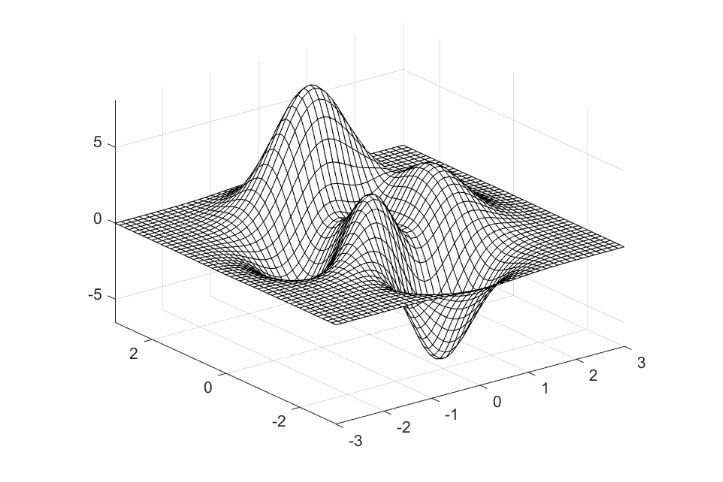
\includegraphics[width=\textwidth,height=\textheight,keepaspectratio]{matlab.png}
  \caption{Visualization of a 3D-mesh in Matlab}
  \label{graphic:mesh-visualization}
\end{figure}

In parallel to MATLAB and R, Python represents the advent of the so-called scripting languages. Scripting languages are programming  languages which offer readability and versatility, along with decoupling from the actual operating system that it is being executed on. System languages, such as C, are designed and used in order to interact directly with the computer hardware, and to constitute data structures from the ground up \citep{ousterhout_scripting_1998}. On the other hand, scripting languages were designed and used in order to connect existing software systems or data sources together, most notably in the early days of shell scripting (such as \lstinline{Bash}, \lstinline{sed} or \lstinline{awk}). Starting with the late 1990s, and the appearance of languages such as Perl\footnote{First version developed in 1987 by Larry Wall} and Python\footnote{First official release in 1991 by Guido Van Rossum}, scripting languages became more widely used by non-programmers who already had data to work with and needed tools to exploit it. In the following decades, the development of additional scientific libraries such as \emph{SciKit}, \emph{NumPy} for mathematics and numerical work or \emph{NLTK} for language processing and social sciences in Python complemented the language's ease of use by providing manipulation of complex scientific concepts \citep{millman_python_2011}, a phenomenon of user-extension which has also been observed in R and MATLAB's ecosystems \citep{moler_history_2020}.

This steady rise of scientific computing has nonetheless highlighted the apparent lack of quality standards in academic software, and how the lack of value judgments on the software written might impact the reliability of the scientific output. Perhaps the most well-known example of such a lack is the one revealed by the leak of the source code of the Climate Research Unit from the University of East Anglia in 2009 \citep{merali_computational_2010}. In the leak, inline comments of the authors, show that particular variable values were chosen to make the simulation run, with scientific accuracy being only a secondary concern. Code reviews of external software developers point out to the code of the CRU leak as being a symptom of the general state of academic software. As Professor Darrel Ince stated to the UK Parliamentary Committee in February 2010:

\begin{quote}
  There is enough evidence for us to regard a lot of scientific software with worry. For example Professor Les Hatton, an international expert in software testing resident in the Universities of Kent and Kingston, carried out an extensive analysis of several million lines of scientific code. He showed that the software had an unacceptably high level of detectable inconsistencies. \citep{committee_disclosure_2010}
\end{quote}

As a response to this realization, the beginning of the 2000s has seen the desire to re-integrate the best practices of software engineering in order to correct scientific software's lack of accuracy \citep{hatton_how_1994}, resulting in the formation of communities such as the Research Software Engineers\citep{woolston_why_2022}. As we have seen above, software engineering had developed on their own since its establishment as an independent discipline and professional field. Such a split, described by Diane Kelly as a "\emph{chasm}" \citep{kelly_software_2007} then had to face the different standards to which commercial software and scientific software were held to. For instance, commercial software must be extensible and performant, two qualities that do not necessarily translate to an academic setting, in which software might be written within a specific, time-constrained, research project, or in which access to computing resources (i.e. supercomputers) might be less of a problem.

Within Landau et. al's conception of the scientific process as the progression from problem to theory, followed by the establishment of a model, the devising of a method, and then on to implemementation and finally to assessment \citep{landau_survey_2011}, code written as academic software is involved in the latter two stages of  method and implementation. Within those two stages, software has to abide by the processes and requirements of scientific research. First and foremost, reproducibility is a core requirement of scientific research in general\footnote{We can date this requirement back to the seventeenth century with Robert Boyle and the Invisible College in England \citep{leveque_reproducible_2012}} and bugs in a scientific software system can lead to radically different ouptuts given slightly different input data, while concealing the origin of this difference. Good academic code, then, is one which defends actively against these, perhaps to the expense of performance and maintainability. This can be addressed by reliable error-handling, regular assertions of the state of the processed data and extensive unit testing \citep{wilson_best_2014}.

Furthermore, a unique aspect of scientific software comes from the lack of clear upfront requirements. Such requirements, in software development, are usually provided ahead of the programming process, and should be as complete as possible. As the activity of scientists is defined by an incomplete understanding of the application domain, requirements tend to emerge as further knowledge is developed and acquired \citep{segal_when_2005}. As a result, efforts have been made to familiarize scientists with software development best practices, so that they can implement quality software on their own. Along with field-specific textbooks\footnote{See \emph{Effective Computation in Physics} \citep{scopatz_effective_2015} or \emph{A Primer for Computational Biology} \citep{oneil_primer_2019} covering similar software-oriented material from different academic perspectives.} the most prominent initiative in the field is \emph{Software Carpentry}, a collection of self-learning and teaching resources which aims at implementing software best practices across academia, for scientists and by scientists. Founded by Greg Wilson, the co-editor of \emph{Beautiful Code}, the organization's title refers directly to equivalents in the field of software development.

We see a convergence of quality standards of broad academic software towards the quality standards of commercial software development\footnote{See Graphbrain at \url{https://github.com/graphbrain/graphbrain} for such an example. The code's organization and formal features are congruent and on par with commercial software.}.  And yet, this convergence is due to, as we have seen, a past divergence between computation and science, as computer science worked towards asserting and pursuing its own field of research. As a subset of science, computer science nonetheless possesses its own specific standards, taking software not as a means to an end, but as the end itself.

\subsubsection{Computation as an end}
\label{subsubsec:computation-end}

Computer scientists are scientists whose work focuses on computation as a means, rather than as a tool. They study the phenomenon of computation, investigating its nature and effects through the development of theoretical frameworks around it. Originally derived from computability theory, as a branch of formal mathematical logic, computation emerged as an autonomous field from work in mechanical design and configuration (Ada Lovelace and Charles Babbage),  work on circuit and language design (C. S. Pierce, Konrad Zuse and John Von Neumann), work on mathematical foundations (Alan Turing and Alonzo Church), information theory (Claude Shannon), systems theory (Norbert Wiener) and expert systems (John McCarthy and Marvin Minsky) \citep{ifrah_universal_2001}. In the middle of such a constellation ranging from mathematical theory to practical electronics, computer science establishes its institutional grounding with the inauguration of the first dedicated academic department at Purdue University in 1962.

From this multifaceted heritage and academic interdisciplinarity, computer scientists identified key areas such as data structures, algorithms and language design as foundations of the discipline \citep{wirth_algorithms_1976}. Though the process, the tracing of the "roots" of computation remained a constant debate as to whether computer science exists within the realm of mathematics, of engineering or as a part of the natural sciences. The logico-mathematical model of computer science contends that one can do computer science without an electronic computer, while the engineering approach of computer science tends to put more practical matters, such as architecture, language design and systems programming (implicitly assuming the use of a digital computer) at the core of the discipline; both being a way to generate and process information as natural phenomenon \citep{tedre_development_2006}.

The broad difference we can see between these two conceptions of computer science is that of \emph{episteme} and \emph{techne}. On the theoretical and scientific side, computer science is concerned with the primacy of ideas, rather than of implementation. The quality of a given program is thus deduced from its formal (in the mathematical sense) properties, rather than its formal (in the aesthetic sense) properties. The first manifestations of such a theoretical focus can be found in the Information Processing Language (1956 by Allen Newell, Cliff Shaw and Herbert Simon), which was originally designed and developed to prove Bertrand Russell's \emph{Principia Mathematica}. While the IPL, as one of the very first programming languages, influenced the development of multiple subsequent languages, some later languages came to be known as logic programming languages, based on a formal logic syntax of facts, rules and clauses about a given domain and whose correctness can be easily proven (see \ref{code:prolog_sample} below for an example of the \emph{Prolog} logic programming language).

\begin{listing}
  \inputminted{prolog}{./corpus/inductive.pl}
  \caption{Prolog sample source}
  \label{code:prolog_sample}
\end{listing}

Due to its Turing-completeness, one can write programs such as language processing, web applications, cryptography or database programming (using the \emph{Datalog} variant of \emph{Prolog}), but its use seems to remain limited outside of theoretical circles in 2021\footnote{See the Stackoverflow Developer survey for popular language uses \url{https://insights.stackoverflow.com/survey/2021}}.

Another programming language shares this feature of theoretical soundness faced with a limited range of actual use in production environments, Lisp—\emph{LISt Processor}—designed to process lists. It was developed in 1958, the year of the Dartmouth workshop on Artificial Intelligence, by its organizator, John McCarthy. Inheriting from IPL, it retained the core idea that programs should separate the knowledge of the problem (input data) and ways to solve it (internal rules), assuming  the rules are independent to a specific problem.

The base structural elements of LISP are not symbols, but lists (of symbols, of lists, of nothing), and they themselves act as symbols (e.g. the empty list). By manipulating those lists recursively—that it, processing something in terms of itself—Lisp highlights even further this tendency to separate computation from the problem domain, and to exhibit autotelic tendencies. This is facilitated by its atomistic and relational structure: in order to solve what it has do, it evaluates each symbol and traverses a tree-structure in order to find a terminal symbol. Building on these features of complex structures with simple elements, Willam Byrd, computer scientst at the University of Utah, describes the following lines of Scheme (a LISP dialect) as "the most beautiful program ever written" \citep{byrd_william_2017}, a Scheme interpreter written in Scheme (\ref{code:scheme_interpreter}):

\begin{listing}
  \inputminted{scheme}{./corpus/interpreter.scheme}
  \caption{Scheme interpreter written in Scheme}
  \label{code:scheme_interpreter}
\end{listing}

The beauty of such a program, for Byrd, is the abilty of these fourteen lines to reveal powerful and complex ideas about the nature and process of computation. As an interpreter, this program can take any valid Scheme input and evaluate it correctly, recreating computation in terms of itself. It does so by showing and using ideas of recursion (with calls to \lstinline{eval-expr}), environment (with the evaluation of the \lstinline{body}) and lambda functions, as used throughout the program. Following Alan Kay, creator of the Smalltalk programming language, Byrd equates the feelings he experiences in witnessing and pondering the program above to those suggested by Maxwell's equations, which constitute the foundation of classical electromagnetism (see \ref{graphic:maxwell-equations}) \citep{kay_conversation_2004}. In both cases, the quality ascribed to those inscriptions come from the simplicity and conciseness of their base elements—making it easy to understand what the symbols mean and how we can compute relevant outputs—all the while allowing for complex consequences for both, respectively, computer science and electromagnetism.

\begin{figure}
  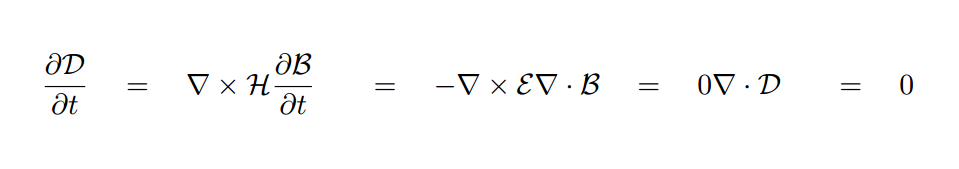
\includegraphics[width=\textwidth,height=\textheight,keepaspectratio]{maxwell.png}
  \caption{Maxwell's equations form a terse, unified basis for electromagnetism, optics and electric circuitry.}
  \label{graphic:maxwell-equations}
\end{figure}

With this direct manipulation of symbolic units upon which logic operations can be performed, Lisp became the language of AI, an intelligence conceived first and foremost as abstractly logical, if not outright algebraic. Lisp-based AI was thus working on what Seymour Papert has called "toy problems"—self-referential theorems, children's stories, or simple puzzles or games \citep{nilsson_early_2009}. In these, the problem and the hardware are reduced from their complexity and multi-consequential relationships to a finite, discreete set of concepts and situations. Confronted to the real world—that is, to commercial exploitation—Lisp's model of symbol manipulation, which proved somewhat successful in those early academic scenarios, started to be applied to issues of natural language understanding and generation in broader applications. Despite disappointing reviews from government reports regarding the effectiveness of these AI techniques, commercial applications flourished, with companies such as Lisp Machines, Inc. and Symbolics offering Lisp-based development and support. Yet, in the 1980s, over-promising and under-delivering of Lisp-based AI applications, which often came from the combinatorial explosion deriving from the list- and tree-based representations, met a dead-end.

"\emph{By making concrete what was formerly abstract, the code for our Lisp interpreter gives us a new way of understanding how Lisp works}", notes Michael Nielsen in his analysis of Lisp, pointing at how, across from the \emph{episteme} of computational truths stands the \emph{techne} of implementation \citep{nielsen_lisp_2012}. The alternative to such abstract, high-level language, is then to consider computer science as an engineering discipline, a shift between theoretical programming and practical programming is Edsger Dijkstra's \emph{Notes on Structured Programming}. In it, he points out the limitation of considering programming exclusively as a concrete, bottom-up activity, and the need to formalize it in order to conform to the standards of mathematical logical soundness. Djikstra argues for the superiority of formal methods through the need for a sound theoretical basis when writing software, at a time when the software industry is confronted with its first crisis.

Within the software engineering debates, the theory and practice distinction had a slightly different tone, with terms like “art” and “science” labeling two different mindsets concerning programming \citep{knuth_art_1997}. As mentioned by Djikstra's example, software engineering suffered from an earlier image of programming as an inherently unmanageable, unsystematic, and artistic activity. There again, many saw programming essentially as an art or craft \citep{tedre_development_2006}, rather than an exact science. Beyond theoretical soundness, computer science engineering concerns itself with efficiency and sustainability, with measurements such as the \emph{O()} notation for program execution complexity. It is not so much about whether it is possible to express an algorithm in a programming language, but whether it is possible to run it effectively, in the contingent environments of hardware, humans and problem domains\footnote{Notably, algorithms in textbooks tend to be erroneous when used in production; only in five out of twenty are they correct \citep{pattis_textbook_1988}.}.

This approach, halfway between science and art, is perhaps best seen in Donald Knuth's magnum opus, \emph{The Art of Computer Programming}. In it, Knuth summarizes the findings and achievements of the field of computer science in terms of algorithm design and implementation, in order to "\emph{to organize and summarize what is known about the fast subject of computer methods and to give it firm mathematical and historical foundations.}" \citep{knuth_art_1997}. The art of computer programming, according to him, is therefore based on mathematics, but nonetheless different from it insofar as it does have to deal with effectiveness, implementation and contingency\footnote{\emph{The Art of Computer Programming} involves a hypothetical computer, called MIX, to implement the algorithms discussed.}. In so doing, Knuth takes on a more empirical approach to programming than his contemporaries, inspecting source code and running software to assess their performance, an approach he first inaugurated for FORTRAN programs when reporting on their concrete effectiveness for the United States Department of Defense \citep{defensetechnicalinformationcenter_dtic_1970}.

Another influential textbook insisting that computation is not to be seen as an autotelic phenomenon is \emph{Structure and Interpretation of Computer Programs}. In it, the authors insist that source code is "\emph{must be written for people to read, and only incidentally for machines to execute}" \citep{abelson_structure_1979}. Still, even when confronted with implementation and the plurality of contingencies of non-mathematical elements which accompanies it, the aesthetic standard in this more engineering approach to computer science is the proportionality between the number of lines of code written and the complexity of the idea explained, as we can see in the series \emph{Beautiful Julia Algorithms} \citep{moss_beautifulalgorithms_2022}. For instance, \ref{code:bubble_sort_julia} implements the Bubble Sort sorting algorithm in one loop rather than the usual two loops in C, resulting in an easier grasping of the concept at hand, rather than being distracted by the idiosyncracy of the implementation. The simplicity of scientific algorithms is expressed even further in \ref{code:nearest_neighbor_julia} the one-line implementation of a procedure for finding a given element's nearest neighbor, a crucial component of classification systems, including AI systems.

\begin{listing}
  \inputminted{julia}{./corpus/bubblesort.jl}
  \caption{Bubble Sort implementation in Julia}
  \label{code:bubble_sort_julia}
\end{listing}

\begin{listing}
  \inputminted{julia}{./corpus/nearest_neighbor.jl}
  \caption{Nearest neighbor implementation in Julia}
  \label{code:nearest_neighbor_julia}
\end{listing}

According to Tedre, computer science itself was split in a struggle between correctness and productivity, between theory and implementation, and between formal provability and intuitive art \citep{tedre_science_2014}. In the early developments of the field, when machine time was expensive and every instruction cycle counted, efficiency ruled over elegance, but in the end he assesses elegance prevailed, as we will see with the evolution of craft within programming in section \ref{sec:craft} below.

In closing, one should note that the \emph{Art} in the title of Knuth's series does not, however, refer to art as a fine art, or a purely aesthetic object. In a 1974 talk at the ACM, Knuth goes back to its Latin roots, where we find \emph{ars}, \emph{artis} meaning "skill.", noting that the equivalent in Greek being τεχνη, the root of both "technology" and "technique.". This semantic proximity helps him reconcile computation as both a science and an art, the first due to its roots in mathematics and logic, and the second

\begin{quote}
  because it applies accumulated knowledge to the world, because it requires skill and ingenuity, and especially because it produces objects of beauty. A programmer who subconsciously views himself as an artist will enjoy what he does and will do it better. Therefore we can be glad that people who lecture at computer conferences speak about the state of the Art. \citep{knuth_computer_1974}
\end{quote}

When written within an academic and scientific context, source code tends to align with the aesthetic standards of software development, valuing reliability, reabability, sustainability, in particular through Greg Wilson's work on the development of software development principles through the Software Carpentry initiative. This alignment can also be seen in a conception of computer science as a kind of engineering, as an empirical practice which can and should still be formalized in order to become more efficient. There, one can turn to Donald Knuth's \emph{Art of Computer Programming} to see the connections between the academia's standards and the industry's standards.

And yet, a conception of computation as engineering isn't the only conception of computer science. Within a consideration of computer science as a  theoretical and abstract object of study, source code becomes a means of providing insights into more complex abstract concepts, seen in the Lisp interpreter, or one-line algorithms implementing foundational algorithms in computer science, similar to this aspect of the hacker ethos. It is this relation to a conception of beauty traditionally associated with mathematics and engineering which we will investigate further to highlight which aesthetic ideals can be ascribed to code. But, first, we complete our overview of code practitioners by turning to the software artists, who engage most directly with source code as a written material through source code poetry.

\pagebreak

\subsection{Poets}
\label{subsec:poets}

Source code poetry is a distinct subset of electronic literature, and software art. One the one hand, electronic literature is a broad field encompassing natural language texts taking full advantage of the dynamic feature of computing to redefine the concept of text, authorship and readership. It encompasses a variety of approaches, including generative literature, interactive fiction, visual poetry, source code poetry and esoteric programming languages, as well as certain aspects of software art. However, we focus here only on the elements of electronic literature which shift their focus from output to input, from executable binary with transformed natural language as a result, to static, latent source.

On the other hand, software art is an umbrella term regrouping artistic practices which engage with the computer on a somewhat direct, material level, whether through hardware\footnote{See Alexei Shuglin's \emph{386 DX} (1998-2013)} or software\footnote{See Netochka Nezanova's \emph{Nebula.M81} (1999)}. This space for artistic experimentation flourished at the dawn of the 20th century, with initiatives such as the \emph{Transmediale} festival's' introduction of a \emph{software art} award between 2001 and 2004, or the \emph{Run\_me} festival, from 2002 to 2004. In both of these, the focus is on projects which incorporate standalone programmes or script-based applications which aren not merely functional tools, but also act as an effective artistic proposition, as decided by the artist, jury and public. These works often bring the normally hidden, basic materials from which digital works are made (e.g. code, circuits and data structures) into the foreground \citep{yuill_code_2004}. Within this realm, code poetry is a form a software art whose execution is only secondary to the work's meaning.

Electronic literature, a form based on the playful \emph{détournement} of the computer's constraints, gets closer to our topic insofar as the poems generated represent a more direct application of the rule-based paradigm to the syntactical output of the program. Starting with Christopher Stratchey's love letters (1953), generated (and signed!) by MUC, the Manchester Univac Computer, computer poems are generated by algorithmic processes, and as such rely essentially on this particular feature of programming: laying out rules in order to synthesize syntactically and semantically sound natural language poems. Here, the rules themselves matter only in relation to the output, as seen by their ratio: a single rule for a seemingly-infinite amount of outputs, with these outputs very often being the only aspect of the piece shown to the public.

These works and their authors build on a longer tradition of rule-based composition, from Hebrew to the Oulipo and John Cage's indeterministic composition, amongst others \citep{cramer_words_2003}, a tradition in which creativity and beauty can emerge from within a strict framework of formal rules. Nonetheless, the source code to these works is rarely released in conjunction with their output, hinting again at their lesser importance in terms of their overall artistic values. If electronic literature is composed of two texts, a natural-language output and a computer-language source, only the former is actually considered to be poetry, often leaving the latter in its shadow (as well as, sometimes, its programmer, an individual sometimes different from the poet). The poem exists through the code, but isn't exclusively limited to the human-readable version of the code, as it only comes to life and can be fully appreciated, under the poet's terms, once interpreted or compiled. While much has been written on electronic literature, few of those commentaries focus on the soundness and the beauty of the source as an essential component of the work, and only in recent times have we seen the emergence of close-readings of the source of some of these works for their own sake\footnote{See the publications in the field of Critical Code studies, Software studies and Platform studies.}. These constitute a body of work centered around the concept of generative aesthetics \citep{goriunova_read_2005}, in which beauty comes from the unpredictable and somewhat complex interplay of rule-based systems, and whose manifestations encompass not only written works, but games, visual and musical works as well.

And yet, the approach of code poets is more specific than broad generative aesthetics: it is a matter of exploring the specific expressive affordances of source code, and the overlap of machine-meaning and human-meaning essential to the correct functioning of code which acts as a vector for artistic communication. Such an overlap of meaning is a specific feature of source code poetry. In a broad sense, code poetry conflates classical poetry (as strict syntactical and phonetical form, combined with poetic expressivity) with computer code, but it is primarily defined by the fact that it does not require the code to be executed, but only to be read by a human. Following the threads laid out by electronic literature, code poetry starts from this essential feature of computers of working with strictly defined formal rules, but departs from it in terms of utility. Code poems are only functional insofar as they are accepted by the intepreter or compiler of the language in which they are written. To the computer, they are indeed functional, in that they are legal and can be parsed; but they do not do anything of \emph{use}. Such formal compliance is only a pre-requisite, a creative constraint, for their human writers.

Within this reliance on creative constraints provided by a computing environment, the emphasis here is on the act of reading, rather than on the act of deciphering, as we have seen with obfuscated code (and in functional code in general). Source code poems are often easy to read, and have an expressive power which operates beyond the common use of programming. Building on Flusser's approach, let us consider poetic thinking as a means to bring concepts into the thinkable, and to crystallize thoughts which are not immediately available to us\footnote{"\emph{In this sense we may say that the intellect expands intuitively. We may, however, define the intuition that results in the production of proper names better, since it is a productive intuition. We may call it “poetic intuition.” The proper names are taken, through this ntuitive activity, from the chaos of becoming in order to be put here (hergestellt), that is, in order to be brought into the intellect.}" \citep{flusser_doubt_2014}}; through various linguistic techniques, poetry allows us to formulate new concepts and ideas, and to shift perspectives.

In their different manifestations, code poems make the boundary between computer meaning and human meaning thinner and thinner, a feature often afforded by the existence and use of higher-level programming languages. Starting with the development of FLOWMATIC in 1955 by Grace Hopper, it was shown that an English-like syntactical system could be used to communicate concepts for the computer to process. From there, programming languages could be described along a gradient, with binary at the lowest end, and natural language (in an overwheling majority, English) at the highest end. This implies that they could be written and read similarly to English, including word order, pronouncation and interpretation, similar to the error-tolerance of human laguages, which doesn't cause the whole communication process to fail whenever a specific word, or a word order isn't understood.

The community of programmers writing in Perl, \emph{perlmonks}\footnote{See their website: \url{https://perlmonks.org/}, with the spiritual, devoted and communal undertones that such a name implies.} has been one of the most vibrant and productive communities when it comes to code poetry. This particular use of Perl started in 1990, when the language creator Larry Wall shared some of the poems written in the language, and it gained further exposition through the work of Shannon Hopkins \citep{hopkins_camels_1992}. The first Perl poem is considered to have been written by Wall in 1990, reproduced in \ref{code:japh_perl}.

\begin{listing}
  \inputminted{perl}{./corpus/japh.pl}
  \caption{Just Another Perl Hacker, japh.pl}
  \label{code:japh_perl}
\end{listing}

Hopkins analyzes the ability of the poem to enable dual understandings of the source—human and machine. Yet, departing from the previous conceptions of source that we have looked at, code poetry does not aim at expressing the same thing to the machine and to the human. The value of a good poem comes from its ability to evoke different concepts for both readers of the source code. As Hopkins puts it:

\begin{quote}
  In this poem, the q operator causes the next character (in this case a newline) to be taken as a single quote, with the next occurrence of that delimiter taken as the closing quote. Thus, the single-quoted line 'Just another Perl hacker' is printed to STDOUT. In Perl, the "unless \$spring" line is mostly filler, since \$spring is undefined. In poetical terms, however, "\$spring" is very important: haiku poetry is supposed to specify (directly or indirectly) the season of the year. As for the q operator, that reads in English as the word "queue", which makes perfect sense in the context of the poem. \citep{hopkins_camels_1992}
\end{quote}

The poem \emph{Black Perl} in \ref{code:black_perl}, submitted anonymously, is another example of the richness of the productions of this community:


\begin{listing}
  \inputminted{perl}{./corpus/black_perl.pl}
  \caption{lBlack Perl, Anonymous, 1990, updated by kck, 2017}
  \label{code:black_perl}
\end{listing}

The most obvious feature of this code poem is that it can be read by anyone, including by readers with no previous programming experience: each word is valid both as English and as Perl. A second feature is the abundant use of verbs. Perl belongs to a family of programming languages grouped under the \emph{imperative} paradigm, which matches a grammatical mood of natural languages, the \emph{imperative mood}. Such mood emphasizes actions to be take rather than, for instance, descriptions of situations, and thus sets a clear tone for the poem. The fact that Perl is based on stating procedures to be executed and states to be changed creates this feeling of relentless urgency when reading through the poem, a constant need to be taking actions, for things to be changed. Here, the native constraints of the programming language interacts directly with the poetic suggestion of the work in a first way: the nature of Perl is that of giving orders, resulting in a poem which addresses \emph{someone} to execute \emph{something}. Still, Perl's flexibility leaves us wondering as to who and what are concerned by these orders. Is the poem directing its words to itself? To the reader? Is Perl just ever talking exclusively to the computer? This ambiguity of the adressee adds to the ominousness of each verse.

Following in the footsteps of the \emph{perlmonks}, additional communities around code poetry have formed, whether in university settings\footnote{Such as Stanford's Code Poetry Slam, which ran between 2014 and 2016, see \url{https://web.archive.org/web/20161024152353/http://stanford.edu/\%7Emkagen/codepoetryslam/} }, or as independent intiatives\footnote{See the Source Code Poetry event, \url{https://www.sourcecodepoetry.com/}}. Beyond collections such as threads and hashtags on Twitter\footnote{See \lstinline{#SongsInCode} at \url{https://twitter.com/search?q=\%2523SongsInCode}}, code poetry also features artistic publications, such as printed anthologies of code poetry in book form \citep{bertram_code_2012} \citep{holden_code_2016}.

Yet, code poems from the 20th century aren't the first time where a part of the source code is written exclusively to elicit a human reaction, without any machinic side-effects. One of the earliest of those instances is perhaps the Apollo 11 Guidance Computer (AGC) code, written in 1969\footnote{Hamilton et. al., 1969, retrieved from https://github.com/chrislgarry/Apollo-11} in Assembly. Cultural references and jokes are peppered throughout the text as comments, asserting computer code as a means of expression beyond exclusively technical tasks\footnote{See also: "Crank that wheel", "Burn Baby Burn"}, and independent from a single writer's preferences, since they passed multiple checks and review processes to end up in the final, submitted and executed document, such as reproduced in \ref{code:numero_mysterioso_asm}.

\begin{listing}
  \inputminted{ca65}{./corpus/numero_mysterioso.asm}
  \caption{AGC source code for the Lunar Landing Guidance Equation, 1969}
  \label{code:numero_mysterioso_asm}
\end{listing}

Code comments allow a programmer to write in their mother tongue, rather than in the computer's, enabling more syntactic and semantic flexibility, and thus reveal a burgeoning desire for programmers to express themselves within their medium of choice.

At the turn of the 1980s, following the transition to programming from an annex practice to full-fledged discipline and profession, and with the development of more expressive programming languages (e.g. Pascal in 1970, C in 1972), software development had grown exponentially\footnote{See Stackoverflow's Developer Profile survey: \url{https://insights.stackoverflow.com/survey/2019\#developer-profile-_-years-since-learning-to-code}}, and fostering practices, communities and development styles and patterns\footnote{From Djikstra's Notes on Structured Programming to Knuth's Literate Programming and Martin's Clean Code}. Source code becomes recognized as a text in its own, which can hold qualities and defects of its own, and to which engineering and artistic attention must be paid. No longer a transitional state from formula to binary, it becomes a semantic material, whose layout, organization and syntax are important to the eyes of its writers and readers. Pushing further into the direction of the visual layout of the code, such an endeavour becomes pursued for its own sake, equally important to the need for a program to be functional.

The Obfuscated C Code Contest\footnote{\url{https://www.ioccc.org}}, starting in 1984, is the most popular and oldest organized production of such code, in which programmers submit code that is functional and visually meaningful beyond the exclusive standards of well-formatted code. If the source code's two meanings of a computer poem was made readily available to interpretation, and if such meanings existed in parallel in the comments of the AGC routines, pointing at the overlay of computer-related semantics (e.g. line numbers) and human-related semantics (e.g. a reference to the biblical number of the beast, 666), obfuscated code is a first foray into closely intertwining these separate meanings in the source code itself, making completely transparent, or completely opaque what the code does just by glancing at it.

\begin{listing}
  \inputminted{c}{./corpus/circle.c}
  \caption{westley.c, entry to the 1988 IOCCC}
  \label{code:circle_c}
\end{listing}

The source code in \ref{code:circle_c}, submitted to the 1988 IOCCC\footnote{Source: \url{https://web.archive.org/web/20131022114748/http://www0.us.ioccc.org/1988/westley.c}} is a procedure which does exactly what it shows: it deals with a circle. More precisely, it estimates the value of PI by computing its own circumference. While the process is far from being straightforward, relying mainly on bitwise arithmetic operations and a convoluted preprocessor definition, the result is nonetheless very intuitive—the same way that PI is intuitively related to PI. The layout of the code, carefully crafted by introducing whitespace at the necessary locations, doesn't follow any programming practice of indentation, and would probably be useless in any other context, but nonetheless represents another aspect of the \emph{concept} behind the procedure described, not relying on traditional programming syntax\footnote{For such a program, see for instance: \url{https://crypto.stanford.edu/pbc/notes/pi/code.html}}, but rather on an intuitive, human-specific understanding\footnote{Concrete poetry also makes such a use of visual cues in traditional literary works.}.

Obfuscating practices, beyond their technical necessities (for security and efficiency), are traditionally tied to hacking practices, prominently with one-liners (the shorter a name, the more obscure and general it becomes). As such, they rely on the brain-teasing process of deciphering, and on the pleasurable, aesthetic experience of resolving and uniting two parallel meanings: what we see in the code, and what it does\footnote{Also known informally as the "Aha!" moment, crucial in puzzle design.}. What we focus on here is the aspect of obfuscation which plays with the different layers of meaning: meaning to the computer, meaning to the human, and different ways of representing and communicating this meaning (from uglifying, to consistent formatting, to depicting a circle with dashes and underscores). While the aesthetics at play in hacking will be further explored below, we focus on the fact that obfuscating code practices, beyond hiding the meaning and the intent of the program, also manifest an attempt to represent such a meaning in different ways, leaving aside traditional code-writing practices and suggesting the meaning of the program by challenging the abilities of human interpretation at play in the process of deciphering programs.

Code poetry values code which, while being functional, expresses more than what it does, by allowing for \emph{Sprachspiele}, languages games where pronounciation, syntax and semantics are playfully composed into a fluid linguistic construct in order to match a human poetic form, such as the haiku, or to constitute a specific puzzle. Relying on the inherent tendency of source code to remain opaque, obfuscated code contests let us see how far can such an opacity of a computer program's effective meaning be sustained.

In this section, we have seen how the set of individuals who write and read code is heterogeneous. Instead, we can see a significant degree of variation between source code written within the context of software engineering, hacking, scientific research and artistic activity. While none of these areas are exclusive of the others—a software developer by day can hack on the weekend and participate in code poetry events—, they do convey different perspectives on how the code is written, and on how it is evaluated. This cursory introduction to each approach has shown that, for instance, software engineers prefer code which is modular, modifiable, sustainable and understandable by the largest audience of possible contributors, while hackers would favor conciseness over expressivity, and tolerate idiosyncracy for the purpose of immediate, functional efficiency. On the other hand, scientific programming favors ease of use, accuracy and reproducibility, sometimes overlapping with software engineering, while code poets explore the semantic tension between a human interpretation and the machine interpretation of a given source code.

These are strands of similarity within apparent diversity. The code snippets in this section show that there is a tendency to prefer a specific group of qualities—readability, conciseness, clarity, expressivity and functionality—even though different types of the aforementionned practices would put a different emphasis on each of those aspects. The question we turn to next, then, is to what extent do these different practices of code writing and reading share common judgments regarding their formal properties? Do hackers and poets agree on some value judgment, and how? To start this investigation, we first analyze programmers' discourses in the following section in order to identify concrete categories of formal properties which might enable a source code to be positively valued for its appearance, before we turn to the aesthetic registers code practicionners refer to when discussing beautiful code to further qualifies these properties.

\pagebreak

\section{Ideals of beauty}
\label{sec:ideals-beauty}

With this overview of the varieties of practices at play amongst those who read and write source code, we will analyze more thoroughly what are the aesthetic standards most value by those different groups. The aim here is to formalize our understanding of which source code is considered beautiful, and to do so at multiple levels. The goal here is to capture both the specific manifestations of beautiful code as specified and enunciated by programmers, as well as the semantic contexts from which these enunciations originate. What we will see is that, while a set of aesthetic values and a set of aesthetic manifestations can be pinpointed precisely, the domains that are mobilized to justify these values are clearly distinct. To do so, we will introduce a discourse analysis framework for the empirical study of the corpus, followed by an examination of the broad fields that these discourses refer to. This will be complemented in Chapter 3 by a a medium-specific reading through critical code studies and rhetorical code studies on one hand, and the work done by conceptual metaphors on the other.

\subsection{Introduction to the Methodology}
\label{subsec:ideals-methodology}

Discourse consists of text, talk and media, which express ways of knowing the world, of experiencing and valuing the world. This study builds on Kintsch and Van Dijk's work on providing tools to analyze an instance of discourse, and is centered around what is said to constitute good source code. While discourse analysis can also be used critically by unearthing which value judgments that occur in power relationships\footnote{See Diana Mullet on Critical Discourse Analysis \citep{mullet_general_2018a}}, we focus here on aesthetic value judgments, as their are first expressed through language. Of all the different approaches to discourse, the one we focus on here is that of \emph{pragmatics}, involving the spatio-temporal and intentional context in which the discourse is uttered. We find this approach particularly fitting through its implication of the \emph{cooperative principle}, in which utterances are ultimately related to one another through communicative cooperation to reveal the intent of the speaker \citep{schiffrin_approaches_1994}. Practically, this means that we assume the position of programmers talking to programmers is cooperative insofar as both speaker and listener want to achieve a similar goal: writing good code. This double understanding—focusing first and foremost on utterances, and then re-examining them within a broader cooperative context—will lead us to encompass a variety of production media (blog post, forums, conferences, text books), in order to depict the cultural background (software practices as outlined above as well as additional factors such as skill levels). Our comprehension of those texts, then, will be set in motion by a a dual movement between local, micro-units of meaning and broader, theoretical macro-structure of the text, and linked by acts of co-reference \citep{kintsch_model_1978}.

Particular attention will be paid to the difference between intentional and extensional meaning \citep{dijk_strategies_1983}. As we will see, some of the texts in our corpus tend to address a particular problem (e.g. on forums, social media or question \& answer platforms), or to discuss broader concepts around well-written code. Particularly,

\begin{quote}
  Figures of speech may attract attention to important concepts, provide more cues for local and global coherence, suggest plausible pragmatic interpretations (e.g., a promise versus a threat), and will in general assign more structure to elements of the semantic representation, so that [meaning] retrieval is easier. \citep{dijk_strategies_1983}
\end{quote}

Following this idea, we will proceed by examining syntactic markers to deduce overarching concepts at the semantic level. Among those syntactic markers, we include single propositions as explicit predicates regarding source code, lexical fields used in those predicates in order to identify their connotations and denotations, as well as for the tone of the enunciations to identify value judgments. At the semantic level, we will examine the socio-cultural references, the \emph{a priori} knowledge assumed from the audience, as well as the semantic entities which compose the theme of the discourse at hand. Finally, the discourses we will examine aren't exclusively composed of natural language, but also of source code extracts, resulting in a hybrid between natural and machine syntax within the same discursive artifact.

In line with John Cayley's analytic framework of structure, syntax and vocabulary \citep{cayley_code_2012}, we can nonetheless echo discourse analysis as applied to natural languages. Cayley's framework highlights essential aspect of analysis which applies both to natural languages and source code: that of the scales at which aesthetic judgment operates. It also provides a bridge with literature and literary studies without imposing too rigid of a grid preventing interdisciplinarity. While it does not immediately acknowledge more traditional literary concepts such as fiction, authorship, literarity, etc., Cayley's framework does leave room for these concepts to be taken into account. Particularly, we will see that the concept of authorship—who writes to whom—will prove to be useful.

Finally, our intepretation of the macrostructures described by Kintsch and Van Dijk will rely extensively on the work done by metaphors as the conceputal level, rather than at the strictly linguistic one. Lakoff and Johsnon's seminal work develops a theory of conceptual metaphors by highlighting their essential dependence on pre-existing cognitive structures, which we associate with already-understood concepts. The metaphor maps a source domain (made up of cognitive structure(s)) to a target domain. In the process, they extend the field of applicability of metaphors from the strictly literary to the broadly cultural: metaphors work because each of us has some conception of those domains involved in the metaphorical process. Metaphors rely in part on a static understanding, resulting in a fixed meaning from the application of a given source to a given target. Some of these sources are called \emph{schemas}, and are defined enough to not be mistaken for something else, but broad enough to allow for multiple variants of itself to be applied to various targets \citep{lakoff_metaphors_1980}, providing both diversity and reliability. As we will see below, their approach allows us to focus not just on textual objects, but on the vast range of metaphors used specifically in computing-related environments. Given that the source of the metaphor should be grounded, with as little invariablity as possible, in order to qualify a potentially ill-defined target domain, this provides us with a first foray into the inherent elusiveness and instability of computing when presented to a broader audience.

Going beyond the role of metaphors manifested in expressions such as \emph{the desktop}, \emph{the mouse}, or \emph{the cloud}, we will explore Lakoff's understanding of the specifically poetic metaphor in Chapter 3 while assessing the linguistic component of computing—source code. For now, we will pay close attention to what programmers are saying about (beautiful) source code, which metaphors they employ to support these value judgments, and why—focusing first on the metaphors \emph{of} source code, before moving, in the next section, to the metaphors \emph{in} source code.

The corpus studied here consists of texts ranging from textbooks and trade manuals to blog posts and online forum discussions\footnote{Specifically, we have gathered 47 different online sources, from forum discussions to blog posts, 26 journal articles from the Association for Computing Machinery, 20 monographs and 1 edited volume, listed in Appendix I. These constitute our primary sources insofar as they are written by practicioners on the topic of good and beautiful code.}. The rationale behind such a broad approach is to constitute a lexical basis for what practicing programmers consider when assessing good code, as expressed in the everyday interactions of online forums and blog posts, but also inclusive of diverse sources of communication, beyond edited volumes. From authoritative sources, such as canonical textbooks or widely-read blog posts from well-known practicioners, to more casual forum exchanges will support the empirical dimension of our research. From this approach, this section will show how there are \emph{specific} ways to qualify well-written code, which are echoed both from bottom-up and from top-down perspectives, and employing recurring references.

\subsection{Lexical Field in Programmer Discourse}
\label{subsec:lexical-fields}

In terms of existing studies of the lexical field programmers use, Erik Pineiro has done significant work in his doctoral thesis. In it, he argues that aesthetics exist from a programmers perspective, decoupled from the final, executable form of the software. While this current study draws on his work, and confirms his findings, it also builds upon it in several ways. First, Pineiro focuses on a narrower corpus, that of the Slashdot.org\footnote{\url{https://slashdot.org}} forums \citep{pineiro_aesthetics_2003} (p. 51). Second, he examines aesthetic judgment from a private perspective of software engineers, separate from other possible aesthetic fields which might enter in dialogue with beautiful code \citep{pineiro_aesthetics_2003} (p.52), such as artists or hackers. Finally, his discussion of aesthetics takes place in a broader context of business management and productivity, while this current study situates itself within media studies and aesthetic philosphy, and its implications within how a certain class of communicative artefacts are considered beautiful. Still, Pineiro's work provides valuable insights in terms of identifying the manifestations and rationales for an aesthetic experience of source code. Thus, we continue his research by highlighting the main adjectives in the lexical field of programmers' discourse.

Already mentioned in Peter Naur's analysis of the practice of programming, \emph{clean} is the first adjective which stands out as a requirement when assessing the form taken by source code. Clean code, he says, is a reference to how easy it is for readers of code to build a coherent theory of the system both described and prescribed by this source code \citep{naur_programming_1985}. This purpose of cleanliness is then completed by a description of the clean form in an analysis of clean code appears a couple of decades later in the title of a series of best-selling trade manuals written by Robert C. Martin and published by Prentice Hall from 2009 to 2021, the full titles of which clearly enunciate their normative aim\footnote{\emph{Clean Code: A Handbook of Agile Software Craftsmanship}, \emph{The Clean Coder: A Code Of Conduct For Professional Programmers}, \emph{Clean Architecture: A Craftsman's Guide to Software Structure and Design}, \emph{Clean Agile: Back to Basics}, \emph{Clean Craftsmanship: Disciplines, Standards, and Ethics}.}. What exactly is cleanliness, in Martin's terms, is nonetheless defined by circumlocutions, relying on contributions from experts. After asking leading programmers what clean code means to them, he carries on in the volume by providing examples of \emph{how} to achieve clean code, while only loosely defining what it is. In general, cleanliness is mostly a definition by negation: it states that something is clean if it is free from impurities, blemish, error, etc. An alternative to this definition which trade manuals such as \emph{Clean Code} use consists in providing examples on how to move from bad, "dirty" code, to clean code through specific, practical guidelines regarding naming, spacing, class delimitation, etc.. Starting at a high-level, some hints can be glimpsed from Ward Cunningham's answer:

\begin{quote}
  You know you are working on clean code when each routine you read turns out to be pretty much what you expected. You can call it beautiful code when the code also makes it look like the language was made for the problem. \citep{martin_clean_2008} (p.10)
\end{quote}

along with Grady Brooch's:

\begin{quote}
  Clean code is simple and direct. Clean code reads like well-written prose. Clean code never obscures the designer’s intent but rather is full of crisp abstractions and straightforward lines of control. \citep{martin_clean_2008} (p.11)
\end{quote}

Cleanliness is tied to expressiveness: it is devoid of any extraneous syntactic and semantic symbols (e.g. it does one thing, and one thing well), in order to let the problem at hand appear, with all its implications. Instead, the tool (i.e. programming languages) disappear at the syntactic level, to enable expressiveness at the semantic level.

Martin echoes Hunt when he advocates for such a definition of clean as lack of additional syntactic information:

\begin{quote}
  Don't spoil a perfectly good program by over-embellishment and over-refinement. \citep{hunt_pragmatic_1999}
\end{quote}

This advice to programmers denotes a conception of clean that is not just about removing as much syntactic form as possible, but which also implies a balance. \emph{Overembellishment} implies excess addition, while \emph{over-refinement} implies, on the contrary, excess removal. This normative approach finds its echo in the numerous quotations of Antoine de Saint-Exupéry's comment on aircraft design\footnote{For instance, see \url{https://news.ycombinator.com/item?id=1640594} and \url{https://twitter.com/codewisdom/status/1353651398337044481}}:

\begin{quote}
  Il semble que la perfection soit atteinte non quand il n'y a plus rien à ajouter, mais quand il n'y a plus rien à retrancher.  \citep{desaint-exupery_terre_1972}\footnote{\emph{ In anything at all, perfection is finally attained not when there is no longer anything to add, but when there is no longer anything to take away, when a body has been stripped down to its nakedness.}, translated by Lewis Galantière in the 1939 edition of \emph{Wind, Sand and Stars}}
\end{quote}

This balance between too much and too little is found in another dichotomy stated by programmers: between simple and clever. Simplicity, argues Jeremy Gibbons, is not only a restraint on the quantity of syntactic tokens (as one could achieve by keeping names short, or aligning indentations), but also a semantic equilibrium at the level of abstracted ideas \citep{gibbons_beauty_2012}. The balance between breadth and depth regarding the task of the code, between the precision of a use-case and its generalization, and its leveraging of external—i.e. supposedly reliable—code is summed up his quoting of Ralph Waldo Emerson at the conclusion of his column:

\begin{quote}
  We ascribe beauty to that which is simple; which has no superfluous parts; which exactly answers its end; which stands related to all things; which is the mean of many extremes. \citep{gibbons_beauty_2012}
\end{quote}

In another ACM publication, Kristiina Karvonen argues for simplicity not just as a design goal, as leveraged by human-computer interface designers, but as a term with a longer history within the tradition of aesthetic philosophy, especially the work of Johann Joachim Winckelmann \citep{karvonen_beauty_2000}. In particular, she stresses the difficulty "to create significant, that is, beautiful works of art with simple means" \citep{karvonen_beauty_2000}. Here, her correlation between \emph{significance} and \emph{pleasant appearance} hints at the semantic role of simplicity, as a means to communicate ideas (i.e. to \emph{signify}) to an audience.

Precisely, simplicity is correlated with clarity (of meaning); if the former refers mainly to the syntactic component (fewer tokens), it enables the non-obfuscated framing of the ideas at play. One example is given in \ref{code:clearer_method_c} by Dave Bush in a post titled  \emph{15 Ways to Write Beautiful Code}.

\begin{listing}
  \inputminted{c}{./corpus/clearer_method.c}
  \caption{Example of clarity differences between two methods.}
  \label{code:clearer_method_c}
\end{listing}

Here, the strive for simplicity leads to removing the brackets, and flipping the boolean check in the if-statement to add a \lstinline{return}. Even though it is, strictly speaking, more characters than the brackets and newline (six characters compared to four), the program becomes cleaner, and thus clearer, he argues, by separating the two branching cases inherent to the use of conditional logic, under the form of an if-statement. In the second version, it is made clear that, if a condition \emph{is}, the execution should stop, and any subsequent statement can entirely disregard the existence of the if-statement; in the first version, the condition that \emph{is not} is entangled with code that should be executed, since the existence of the if-statement has to be kept in mind until the closing bracket \citep{bush_15_2015}.

As a corollary to clarity stands obfuscation. It is the act, either intentional or un-intentional, to complicate the understanding of what a program does by leading the reader astray through a combination of syntactic techniques, a process we have already seen in the works of the IOCCC above. In its most widely applied sense, obfuscation is used for practical production purposes: reducing the size of code, and preventing the leak of proprietary information regarding how a system behaves. For instance, the JavaScript source code in \ref{code:home_js} is obfuscated through a process called \emph{minification} into the source code in \ref{code:home_minified_js}

\begin{listing}
  \inputminted{js}{./corpus/home.js}
  \caption{home.js (before minification)}
  \label{code:home_js}
\end{listing}

\begin{listing}
  \inputminted{js}{./corpus/home_minified.js}
  \caption{home.js (after minification)}
  \label{code:home_minified_js}
\end{listing}

This process of obfuscation has very clear, quantitative assessment criterias, such as the size of the source code file and cryptographic complexity \citep{pellet-mary_co6gc_2020}. Nonetheless. obfuscation can also be valued as a positive aesthetic standard, of which the IOCCC is the most institutionalized guarantor. These kinds of obfuscations, as Mateas and Montfort analyze, involve the playful exploration of the intertwinings of syntax and semantics, seeing how much one can bend the former without affecting the latter. These textual manipulations, they argue, possess an inherently literary quality:

\begin{quote}
  Obfuscation and weird languages invite us to join programming contexts to the literary contexts that must obviously be considered when evaluating literary code. They also suggest that coding can resist clarity and elegance to strive instead for complexity, can make the familiar unfamiliar, and can wrestle with the language in which it is written, just as much contemporary literature does. \citep{mateas_box_2005}
\end{quote}

Such literary connection can also be seen in Noël Arnaud's work \emph{Poèmes Algol} \citep{arnaud_poemes_1968}, in which he uses the constructs of the language Algol 68 in order to evoke in the reader something different than what the program actually does (i.e. fail to execute anything meaningful). Here, obfuscation is can be considered a literary value, as opposed to other domains, such as the scientific or the architectural, where it is both considered exclusively negatively.

Another insight on simplicity and programming regarding the communication of ideas is hinted at by Richard P. Gabriel in his use of the concept of \emph{compression} in both poetry and programming, there is a desire to increase the semantic charge (or significance, in Karvonen's terms) all the while reducing the syntactic load (or the quantitity of formal tokens). One of those extraneous loads is explanation, as pointed out online by user Mason Wheeler:

\begin{quote}
  When it requires a lot of explanation like that, it's not "beautiful code," but "a clever hack." \citep{stackoverflow_how_2013}
\end{quote}

This answer, posted on the software engineering \emph{Stack Exchange} forum, in response to the question "How can you explain "beautiful code" to a non-programmer?" \citep{stackoverflow_how_2013}, not only highlights the need to be self-explanatory, but also points at a quality departing form simplicity—cleverness.

Cleverness is often found, and sometimes derided, in examples of code written by hackers, since it unsettles this balance between precision and generality. Clever code would tend towards exploiting particularities of knowledge of the medium (the code) rather than the goal (the problem). Hillel Wayne presents the snippet of Python code in \ref{code:is_unique_python} as an example of bad clever code:

\begin{listing}
  \inputminted{python}{./corpus/unique.py}
  \caption{Method to check for the uniqueness of array elements}
  \label{code:is_unique_python}
\end{listing}

Here, the knowledge of how the \lstinline{set()} function in Python behaves, is required in order to understand that the \lstinline{is_unique()} function returns whether all the elements of the given list are unique. A programmer without familiarity with Python would be unable to do so without consulting the Python documentation (i.e. requiring extraneous explanation).

Hillel elaborates on the difference between "bad" clever code\footnote{See, for instance, Duff's device, an idiosyncratic and language-specific way to speed up loop unrolling in C. The author himself feels "a combination of pride and revulsion at this discovery" \citep{duff_tom_1983}}, which is essentiall read-only due to its idiosyncracy and reliance on tacit knowledge, and "good" clever code, and such distinction corroborates our previous observations regarding beautiful code as a means for expression of the problem domain. His example is that the problem of sorting the roughly 300 million U.S. american citizens by birthdate can be made considerably more efficient by cleverly considering that no U.S. american citizen is older than 120 years, whereby radically reducing the computation space.

Meanwhile, cleverness is a valued attribute in the context of hacker code, putting more emphasis on the technical solution than on the problem domain, as we have seen above. A salient is example was the 1994 \lstinline{smr.c} entry to the IOCCC, which aimed at being the smallest self-reproducing program \citep{kanakarakis_international_2022}. An exact reproduction of the source code can be found in \ref{code:smr_c}

\begin{listing}
\inputminted{c}{./corpus/smr.c}
  \caption{smr.c}
  \label{code:smr_c}
\end{listing}

Consisting of a file weighing zero bytes, \lstinline{smr.c} provides both a clever reduction of the problem domain, and a clever understanding of what C compilers would effectively accept or not as a valid program text \citep{kanakarakis_international_2022a}. Because it has since been banned under the rules of the IOCCC, this source code entirely renounces any claim to a more general application, and finds its aesthetic value only within a specific community.

Coming back to simplicity, we can define more precisely such a qualifier of source code to be \emph{an exact fit to the problem}: without being too precise, or too generic, displaying an understanding of and a focus on the application domain, rather than the applied tools. William J. Mitchell sums it up in his introductory textbook for graphics programming:

\begin{quote}
  Complex statements have a zen-like reverence for perfect simplicity of expression. \citep{mitchell_art_1987}
\end{quote}

Programmers hold the idea of reaching a conceptual revelation through the reduction of complex styntactical assemblages. This strive towards attaining an inverse relationship between the complexity of an idea and the means to express it is contiguous to another related criteria for beautiful source code present in programmers' discourse: \emph{elegance}. Leslie Valiant, recipient of the Turing Award in 2010, considers elegance as the explanatory power of simple principles, which might only appear \emph{a posteriori}—a solution can only be qualified as elegant once it has been found, and very rarely during the process of its development\citep{anthes_beauty_2011}. Chad Perrin, in his article \emph{ITLOG Import: Elegance}, first approaches the concept as a negation of the gratuitous, a means to reduce as much as possible the syntactic footprint while keeping the conceptual footprint intact:

\begin{quote}
  In pursuing elegance, it is more important to be concise than merely brief. In a general sense, however, brevity of code does account for a decent quick and dirty measure of the potential elegance that can be eked out of a programming language, with length measured in number of distinct syntactic elements rather than the number of bytes of code: don't confuse the number of keystrokes in a variable assignment with the syntactic elements required to accomplish a variable assignment. \citep{perrin_itlog_2006}
\end{quote}

Perrin also hints at the additional meaningfulness of elegance, as he compares it to other aesthetic properties, such as simplicity, complexity or symmetry. If simplicity inhabits a range between too specific and too general, he describes an elegant system as exactly appropriate for the task at hand, echoing others' definition of clean or simple source code. Elegance, he says, relies on strong, underlying principles, but is nonetheless subject to its manifestation through a particular, linguistic interface. While he touches at length on the influence of progamming languages in the possibility to write elegant source code, we will only address this question in Chapter 4.

Donald Knuth adds another component required to achieve elegance in software: along with leanness of code and the suitability of the language, he adds that elegance necessitates a clear definition of the problem domain \citep{fuller_software_2008}. Along with the appropriateness of the linguistic tooling, one can see here that the representation of the data which is then going to be processed by the executed source code also matters. Indeed, source code is not only about expressing dynamic processes, but also about translating the problem domain into formal static representations which will then be easy to operate on.

This aspect of implying underlying principles is also present in Bruce McLennan's discussion of the concept. As he approaches it through the dual lens of structural engineering, this indicates that he also considers elegance as a more profound concept which can manifest itself across disciplines, both as a way of making, and as a way of thinking \citep{mclennan_who_1997}. He defines his \emph{Elegance Principle} as:

\begin{quote}
  Confine your attention to designs that \emph{look} good because they \emph{are} good. \citep{mclennan_who_1997}
\end{quote}

Such a definition relies heavily on the sensual component of elegance: while an underlying property of, at least, human activities, it must nonetheless be manifested in some perceptible way. On \emph{Stackexchange}, user \emph{asoundmove} corroborates this conception of achieving a simple and clean system where any subsequent modification would lead to a decrease in quality:

\begin{quote}
  However to me beautiful code must not only be necessary, sufficient and self-explanatory, but it must also subjectively feel perfect \& light. \citep{stackoverflow_how_2013}
\end{quote}

Once again connecting simplicity (under the guise of necessity and sufficiency), the perception of elegance is also related to a subjective feeling of adequacy, of fitting. Including some of the definitions of simplicity we have seen so far, Paul DiLascia, writing in the Microsoft Developer Network Magazine, illustrates his conception of elegance—as a combination of simplicity, efficiency and brilliance—with recursion \citep{dilascia_end_2019}, as seen in \ref{code:factorial_c}.

\begin{listing}
  \inputminted{c}{./corpus/factorial.c}
  \caption{Use of recursivity in the computation of a factorial}
  \label{code:factorial_c}
\end{listing}

Recursion, or the technique of defining something in terms of itself, is a positively valued feature of programming \citep{abelson_structure_1979}, which we have seen an example of in \ref{code:scheme_interpreter}. In so doing, it minimizes the number of elements at play and constrains the problem domain into a smaller set of moveable pieces. Another example, provided in the same \emph{Stackexchange} discussion is the \lstinline{quicksort} algorithm, which can be implemented recursively or iteratively, with the former being significantly shorter (see \ref{code:recursion_iteration_csharp})

\begin{listing}
  \inputminted{csharp}{./corpus/recursive_iteration.cs}
  \caption{Comparison two functions, one using recursion, the other one using iteration, https://stackoverflow.com/a/12553314/4665412}
  \label{code:recursion_iteration_csharp}
\end{listing}

Concluding this survey of how programmers perceive, define and exemplify elegance in source code, we can follow Mahmoud Efatmaneshik and Michael J. Ryan who, in the IEEE Systems journal, offer a definition of elegance which relies both on a romantic perception—including subjective perception, "gracefulness", "appropriateness" and "usability"—and practical assessment with terms such as "simple", "neat", "parsimonious" or "efficient" \citep{efatmaneshnik_definitions_2019}. In doing so, they ground source code aesthetics as a resolutely dualistic norm, between subjectivity and objectivity, qualitative and quantitative\footnote{A duality we will investigate further through the prism of human and machine understanding in Chapter 2}.

And yet, rather than subjectivity and objectivity being opposites, one could also consider them as contingent. Due to the interchangeability in the use of the some of the terms we have seen by programmers, both qualitative—in terms of the language used—and quantitative—in terms of the syntax/semantics ratio—assessments of source seem to be complementary in considering it elegant. If \emph{clean}, \emph{simple}, \emph{elegant} seem to overlap, it is because they all seem to point at this maximization of meaning while appropriately minimizing syntax.

A complementary approach to understand what programmers mean when they talk about beautiful code is to look beyond the positive terms used to qualify it, and shift our attention to how other terms are used negatively. We have already touched upon qualifiers such as clever, or obfuscated, which have ambiguous statuses depending on the community that they're being used in—specifically hackers and literary artists. Further examination of negative qualifiers will enrich of understanding of what constitutes good code.

One of those hints comes from satirical accounts of how to write bad code. For instance, Green's post on \emph{ How To Write Unmaintainable Code} suggests new kinds of obfuscation, such as double-naming in \ref{code:green_unmaintainable} or semantic interactions in \ref{code:green_unmaintainable_2}. The core ideas presented here revolve around creating as much friction to understanding as possible, by making it "as hard as possible for [the reader] to find the code he is looking for" and "as awkward as possible for [the reader] to safely ignore anything." \citep{green_how_2006}.

\begin{listing}
  \inputminted{python}{./corpus/unmaintainable.py}
  \caption{Choose variable names that masquerade as mathematical operators}
  \label{code:green_unmaintainable}
\end{listing}

\begin{listing}
\inputminted{c}{./corpus/unmaintainable_2.c}
  \caption{Code That Masquerades As Comments and Vice Versa}
  \label{code:green_unmaintainable_2}
\end{listing}

By looking at it from the opposite perspective of highly-confusing code, we see best how carefully chosen aesthetics, under the values of simplicity, clarity, cleanliness and elegance intend first and foremost to help alleviate human cognitive friction and facilitate understanding of what the program is doing. The opposite amounts to playing misleading tricks.

Along with this mental property, programmers have another way to refer to code that does not meet aesthetic criteria, which is also relates primarily to a non-cognitive aspect of source code, by refferring to material properties.

For instance, \emph{Spaghetti code} refers to a property of source code where the syntax is written in such a way that the order of reading and understanding is akin to disentangling a plate of spaghetti pasta. While still linear in execution, this linearity loses its cognitive benefits due to its extreme convolution, making it unclear what starts and ends where, both in the declaration and the execution of source code. Rather than using a synonym such as \emph{convoluted}, the image evoked by spaghetti is particularly vivid on a sensual level, as a slimy, vaguely structured mass, even if the actual processes at play remain eminently formal \citep{steele_macaroni_1977}. Such a material metaphor can also be in Foote and Yoder's description of code as a "big ball of mud":

\begin{quote}
  A Big Ball of Mud is a haphazardly structured, sprawling, sloppy, duct-tape-and-baling-wire, spaghetti-code jungle. These systems show unmistakable signs of unregulated growth, and repeated, expedient repair. Information is shared promiscuously among distant elements of the system, often to the point where nearly all the important information becomes global or duplicated. \citep{foote_big_1997}
\end{quote}

A broader approach to these sensual perceptions of code involve the reference to \emph{code smells}. These smells are described by Martin Fowler as "surface indications that usually corresponds to a deeper problem in the system" \citep{fowler_refactoring_1999}. They are aspects of source code which, by their syntax, might indicate deeper semantic problems, without being actual bugs. The name code smell evokes the fact that their recognition happens through intuition and experience of the programmer reading the code, rather than through careful empirical analysis\footnote{It should be noted that more recent computer science research has recently also focused on developing such empirical techniques \citep{rasool_review_2015}, even though their practical usefulness is still debated \citep{santos_systematic_2018}}. This points to a practice-based value system to evaluate the quality of source code, rather than to an evidence-based system, itself circling back to the qualifications of elegance discussed above, evaluated both as quantitative metric and as qualitative one.

In this section, we clarified the main terms used in programmers' discourse when discussing aesthetically pleasant code. Basing our interpretation of the gathered sources through discourse analysis, we specifically assumed a cooperative principle, in which all participants in the discourse intend to achieve writing the best source code possible. This analysis has confirmed and updated the findings of Piñeiro's earlier study. Across textbooks, blog posts, forums posts and trade books, the aesthetic properties of code are widely acknowledged and, to a certain extent, consistent in the adjectives used to qualify it (clean, elegant, simple, clear, but also clever, obscure, or dirty).

While there is a consistency in describing the means of beautiful code, by examining a lexical field with clear identifiers, this analysis also opens up additional pathways for inquiry. First, we see that there is a relationship between formal manifestations and cognitive burden, insofar as aesthetics help alleviate such a burden. Beautiful code makes the ideas which are embedded in it, and the world in which the code aims to translate and operate on, more accessible to the reader. Additionally, the negative adjectives mentioned when referring to the formal aspects of code (smelly, muddy, entangled) are eminently \emph{materialistic}, indicating some interesting tension between the ideas of code, and the sensuality of its manifestation.

Moving beyond strict lexical tokens, we have seen in the breadth of responses in a programmer's question of "How can you explain "beautiful code" to a non-programmer?" \citep{stackoverflow_how_2013}, programmers also rely multiple aesthetic domains to which they refer: from engineering and literature to architecture and mathematics. We now turn to an investigation of each of these domains, and of how they can be related to code.

\pagebreak

\section{Aesthetic domains}
\label{sec:aesthetic-domains}

This examination of which qualifiers programmers use when they relate to the aesthetic qualities  of source code (the way it looks) or the aesthetic experience that it elicits (the way they feel) has shown both a certain degree of coherence, and a certain degree of elusiveness. Subjectively, programmers associate their experience of encountering well-written code as an aesthetic one. However, on a normative level, things become a little more complicated to define: as we have seen in the previous section's discussion of forum exchanges, beauty in source code is not and explicited in and of itself, but is best illustrated by referring to to other domains.

The next step that we propose is to inquire into these specific domains, to examine in which capacity they are being summoned in relation to code, and how they help us further delineate the aesthetic qualities which belong to source code. The assumption here is that, following Neil Postman, a medium is a means of expression, and different mediums can support different qualities of expression \citep{postman_amusing_1985}. Since there seems to be some specific ways in which code can be considered beautiful, these contingent domains, and the specific parts of these domains which create this contingency, will prepare our work of defining source code-specific aesthetic standards.

To do so, then, we will look at the three domains most often conjured by programmers when they mention the sensual qualities of, or the aesthetic experiences elicited by, source code: literature, mathematics and architecture. While there are accounts of parallels between programming and painting \citep{graham_hackers_2003} or programming and music\citep{mclean_hacking_2004}, these refer rather to the painter or musician as an individual, rather to the specific medium, and there are, to the best of our knowledge, no account of code being like sculpture or film, for instance.

\subsection{Literary Beauty}
\label{subsec:literary-beauty}

The most striking, and obvious similarity between code and another medium of expression is that of literature: perhaps because they both require, fundamentally, the use of alphanumeric characters laid out on a two-dimensional plane. Similarly, syntax and semantics interplay in order to convey meaning to a reader. \emph{Code as literature}, then, focuses on this intertwining of natural language and computer language, on its narrative, rhetorical and informative properties, and even on its ability to mimick the traditional forms of poetry.

\subsubsection{Code as a linguistic practice}
\label{subsubsec:code-linguistic}

In \emph{Geek Sublime}, Vikram Chandra, novelist and programmer, lays out the deep parallels he sees between code and human language, specifically sanskrit. While stopping short of claiming that code is literature, he nonetheless makes the claim that sanskrit is, as a set of generative linguistic rules to compose meaning, a distant ancestor to computer code \citep{chandra_geek_2014}, a fact corroborated by Agathe Keller in her studies of the Āryabhaṭa \citep{keller_textes_2021}. Sanskrit, like computer code, relies on context-free rules and exhibits similar properties as in code, such as recursion and inheritance.

With a similar syntactic structure between sanskrit and code, the former also exhibits a "\emph{search for clear, unambiguous understanding}" through careful study, a goal equally shared by the writers of source code, as we have seen above. Specifically, the complexity of the linguistic system presented both in sanskrit and in machine language implies that enjoyment of works in either medium happens not through spontaneous, subjective appreciation, but through "conoisseurship", resulting from education, experience and temperament \citep{chandra_geek_2014}.

Similarly, in \emph{Words Made Flesh: Code and Cultural Imagination}, Florian Cramer touches upon code's ability to \emph{do} things, in order to inscribe it differently in a historical development of linguistics, connecting it to the symbolical works of the kabbalah and Lebniz's \emph{Ars Combinatoria}. Code, according to Cramer, is linguistic, not just because it is made up of words, but because it \emph{acts upon} words, influencing what we consider literature and human-language writing:

\begin{quote}
  The step from writing to action is no longer metaphorical, as it would be with a semantic text such as a political speech or a manifesto. It is concrete and physical because the very code is thought to materially contain its own activation; as permutations, recursions or viral infections. \citep{cramer_words_2003}
\end{quote}

Those permutations and recursions are used in the different ways: natural language writers have attempted to apply formulas, or algorithms, to their works, from the Oulipo's \emph{Poèmes Algol} to Cornelia Sollfrank's \emph{Net.Art Generator}. The properties that Cramer identifies in machine languages, tensions between totality and fragmentation, rationalization and occultism, hardware and software, syntax and semantics, artificial and natural, are ascribed to the newest development of the interaction between program and expression, for instance through the shape of those combinatorial poetics \citep{cramer_words_2003}. This resemblance, or \emph{Familienähnlichkeit}, to other forms of linguistic expression, is explored further by Katherine Hayles' work on speech, writing and code. Specifically, she sees the linguistic practices of humans and intelligence machines as influencing and interpenetrating each other, considering code as language's partner\footnote{Hayles's work on posthumanism should be acknowledged here, as she envisions the human brain as a platform on which code runs, both natural codes such as sanskrit, or more computational forms of codes.}.

Specifically, Hayles looks at how both literature and code can be expressive in a syntagmatic manner as well as in a paradigmatic manner. In the former, the meaning spread across the words of a sentence is considered fixed in literature, while it is dynamically generated in source code, depending of the execution state and the problem domain. In the latter, the meaning across synonyms in a (program) text is always potential in literature, but always present in code \citep{hayles_print_2004}—highlighting different levels of interpretation. If code is a form of linguistic system, then it is a dynamic one in which the semantic charge is at least as volatile as in literature, but which possesses an additional \emph{dimension}, as orality, literacy and digitality succeed each other by bringing the specificity of their media.

Code is thus considered a linguistic system in the technical sense, having a syntactic ruleset operating on words, it seems to also be a linguistic system in the cultural sense. As such, it deals with the occult, the magical and the obscure, but also exhibits a desire to communicate and execute unambiguous meaning.

This desire for explicit communication led literacy scholars to investigate source code's relationship to rhetoric. While digital systems seem to exhibit persuasive means of their own \citep{bogost_rhetoric_2008} \citep{frasca_simulation_2013}, the code that underpins them also presents rhetorical affordances. The work of Kevin Brock and Annette Vee in this domain has shown that source code isn't just a normative discourse to the machine, but also an argumentative one with respect to the audience: it tries to persuade fellow programmers of what it is doing. From points being made in large-scale software such as Mozilla's Firefox web browser, to more specific styles in job interviews, source code presents worldviews in its own specific syntax \citep{brock_rhetorical_2019}.

The connections of code to linguistics happens thus at the technical, media, and cultural levels, insofar as it can allow for the expression of ideas and arguments, straddling the line between the rational and the evocative. We now turn more specifically to two instances of program code being considered a literary text, by leading programmers in the field: Yukihiro 'Matz' Matsumoto and Donald Knuth.

\subsubsection{Code as text}
\label{subsubsec:code-text}

Perhaps the most famous reference to code as a literary object is to be found in Donald Knuth's \emph{literate programming}. In his eponymous 1984 article in \emph{The Computer Journal}, Knuth advocates for a practice of programming in which a tight coupling of documentation with source code can allow one to consider programs as "works of literature" \citep{knuth_literate_1984}. It is unclear, however, what Knuth entails when he refers to a work of literature\footnote{For instance, he refers in the rest of the article as "constructing" programs, rather than "writing" them.}.

Literate programming, a direct response to \emph{structured programming}, enables the weaving of natural language blocks with machine language blocks, in order to be able to comile a single source into either a typeset documentation of the program, using the TeX engine\footnote{In which this current thesis is written.}, or into a source file for a Pascal compiler. The literary, here, is only a new set of tools and practices of writing which result in a \emph{publishable work}, rather than a \emph{literary work}, in which the program is described in natural language, with source code being interspersed as snippets throughout. While this approach fits aptly within Knuth's interest in typesetting and workflows of scientific publications, it does not explicitly address the relationship between literature and programming beyond this.

Still, his aim remains to support a clear understanding of a program by its reader, particularly emphasizing the complexity of such tasks. If he proposes something with regards to literature, it is in the process of meaning-making through reading, and its cognitive implications:

\begin{quote}
  This feature of WEB is perhaps its greatest asset; it makes a WEB-written program much more readable than the same program written purely in PASCAL, even if the latter program is well commented.  [...] a programmer can now view a large program as a web, to be explored in a psychologically correct order is perhaps the greatest lesson I have learned from my recent experiences. \citep{knuth_literate_1984}
\end{quote}

For Knuth, then, code is a text: both in the traditional, publisher-friendly way, but also in a new, non-linear way. This attention to the materiality of the program—layout, typesetting—foresees subsequent technological solutions to allow natural language and machine language to co-exist\footnote{See JavaDocs, Go docs, Jupyter Notebooks}.

This new way to approach (digital, hybrid) texts is expressed by Yukihiro Matsumoto, the creator of the Ruby programming language, in his notion of \emph{Code as an Essay} \citep{oram_beautiful_2007}. While he doesn't deal directly with questions of eloquence and rhetoric, as opposed to Brock and Vee, it does however start from the premise that code is a kind of text, insofar as it has an a message being conveyed in a written form to an audience. However, it is not a kind of text which has a specific author, or a specific finite state:

\begin{quote}
  Most programs are not write-once. They are reworked and rewritten again and again in their lived. Bugs must be debugged. Changing requirements and the need for increased functionality mean the program itself may be modified on an ongoing basis. During this process, human beings must be able to read and understand the original code.
\end{quote}

This conception, in which a text remains open to being modified further by subsequent voices, thus minimizing the aura of the original version, and possibly diluting the intent of the original author, echoes the distinction made by Roland Barthes between a \emph{text lisible} (readerly text) and \emph{texte scriptible} (writerly text). While the former aligns with classical conceptions of literature, with a clear author and life span for the literary work, the latter remains open to subsequent, subjective appropriations.

This appropriation is such that a modified program text does not result in a finite program text either; due to its very low barrier to modification and diffusion, program texts can act almost as a dialogue between two programmers. As Jesse Li puts it, building the linguistic theory of Volonishov and Bakhtin:

\begin{quote}
  The malware author is in dialogue with the malware analyst. The software engineer is in dialogue with their teammates. The user of a piece of software is in dialogue with its creator. A web application is in dialogue with the language and framework it is written in, and its structure is mediated by the characteristics of TCP/IP and HTTP. And in the physical act of writing code, we are in dialogue with our computer and development environment. \citep{li_where_2020}
\end{quote}

It is to support this act of dialogue, supported by code's affordance of rapid modification and redistribution, that Matusmoto highlights simplicity, brevity—his term for elegance— and balance—insofar as no one dimension alone is enough—as means to achieve writing beautiful code. His last criteria, lightness, applies not to the code being written, but to the language being used to write such code, adding one more dimension to the dialogue: between the writer(s), the reader(s) and the language designer(s), an additional aspect we will return to in chapter 3.

These two examples show us that source code can be considered a text, if not a literary work which needs to accomodate a hybrid of natural and machine languages, new modes of diffusion, and countless possibilities for being rewritten. In this technological environment of programming languages (from WEB to Ruby), the aim is to facilitate the understanding of what the program does, and of what it should do.

Beyond these theoretical and functional conceptions of code's textuality, a last approach to the literariness of source code can be found in the works of code poetry, in which this ambiguity is embraced.

\subsubsection{Code poetry}
\label{subsubsec:code-poetry}

Daniel Temkin, in his \emph{Sentences of Code Art}\footnote{A direct reference to Sol Lewitt's \emph{Sentences on Conceptual Art}.}, suggests the ways in which code art (encompassing code poetry, esoteric languages and obfuscated code, among others) touches on code's linguistic features mentioned by Chandra and Cramer, while coming at it from a non-functional perspective, radically opposed to Knuth and Matsumoto.

\begin{quote}
  The ambiguity of human language is present in code, which never fully escapes its status as human writing, even when machine-generated. We bring to code our excesses of language, and an ambiguity of semantics, as discerned by the human reader. \citep{temkin_sentences_2017}
\end{quote}

The artists whose main medium is source code explore the possibilities of meaning-making through mechanisms usually associated with poetry. For instance, code art is focused on the evokative possibilities of machine languages, and away from its exactness. This is a step further in a direction of semantic possibilities hinted at by Richard P. Gabriel when he mentions the parallels between writing code and writing poetry. In an interview with Janice J. Jeiss, he states:

\begin{quote}
  I'm thinking about things like simplicity -- how easy is it going to be for someone to look at it later? How well is it fulfilling the overall design that I have in mind? How well does it fit into the architecture? If I were writing a very long poem with many parts, I would be thinking, "Okay, how does this piece fit in with the other pieces? How is it part of the bigger picture?". When coding, I'm doing similar things, and if you look at the source code of extremely talented programmers, there's beauty in it. There's a lot of attention to compression, using the underlying programming language in a way that's easy to penetrate. Yes, writing code and writing poetry are similar.  \citep{jeiss_poetry_2002}
\end{quote}

Further exploring the semantic possibilities of considering source code as a possible medium for poetic expression, one can turn to the analyses of code poems in publications such as Ishaac Bertram's edited volume, \emph{code \{poems\}} and Nick Montfort's collected poems in \emph{\#!}.

In the former's foreword, Jamie Allen develops further this ability to express oneself via machine languages, considering that programmers can have "\emph{passionate conversations in Python}" or "\emph{with a line in a text file [...] speak directly to function, material action, and agency}" \citep{bertram_code_2012}. This is done, not by relying on the computer as a generative device, but by harnessing from the form and subject matter of those very machine languages which subsequently can exhibit those generative properties. Focusing on the language part of the machine allows for an interplay between human and machine meanings.

Still, machine semantics are nonetheless considered as an essential device in writing code poetry, and exploring concepts that are not easily grasped in natural languages—e.g. hoisting or destructuring assignment. Additionally, the contrast between the source representation of the poem and its execution can add to the poetic tension, as we see in Nick Montfort's \emph{All The Names of God} (2010) (source in \ref{code:all_the_names_of_god}, and output in \ref{output:all_the_names_of_god}).

\begin{listing}
\inputminted{perl}{./corpus/all_the_names_of_god.pl}
  \caption{All The Names of God, Nick Montfort, 2010, source}
  \label{code:all_the_names_of_god}
\end{listing}

\begin{listing}
  \inputminted[breaklines=true,breakanywhere]{text}{./corpus/all_the_names_of_god.txt}
  \caption{All The Names of God, Nick Montfort, 2010, Selected output}
  \label{output:all_the_names_of_god}
\end{listing}

This poem is the object of close literary critical examination by Maria Aquilina, who notes that \emph{[t]he contrast between the economical minimalism of the program and the ordered but infinite series of letter combinations it produces is one of the aspects that make the poem striking} \citep{aquilina_computational_2015}. Building on philosophy and literary theorists, Aquilina situates the expressive power of the poem in its engagement with the concept of \emph{eventualization}, locating the semantic load of the poem in its existence both in a human-perception of the non-human (e.g. computer time) and the dialogue between source, output and title \citep{aquilina_computational_2015}.

Not only is there an aesthetic of minimalism present in the source (to which Perl lends itself perfectly), the output also represents the \emph{depth} (in Hayles's sense) of the medium of writing. As we have seen above, a literary conception of source code aesthetic can, under certain circumstances, find its quality not just the limit in characters, but in the relationship between such a limit and the expansiveness of the ideas expressed.

From software developers to artists, different kinds of writers seem to equate code as a text, bringing forth multiple reasons to justify such a connection. Beyond the fact that source code is made up of textual characters, we see that these conceptions of code as literature are multiple`'. On the one side, it is focused on its need to communicate explicit concepts related to its function (Knuth, Matsumoto, Brock), all the while embracing the semantic ambiguity which exists in the use of natural language tokens, backed-up by the potential executable semantics enabled by its machine nature (Cramer, Hayles, Montfort, Temkin).
The last example, the tension between \emph{All The Names of God}'s source and output, between notation and ideas, suggests us to look at this kind of elegance not through a literary lens, but through a scientific one—another domain conjured by code writers and readers.

\subsection{Scientific beauty}
\label{subsec:scientific-beauty}

Having strong roots in scientific thought and practice, via the connection of computer science, the aesthetic experiences of source code are also related to the scientific domain. Nonetheless, it seems to exist in two distinct ways: whether code is beautiful in a similar way that mathematics is, or wether code is beautiful according to equivalent principles at play in engineering.

\subsubsection{Mathematics}
\label{subsubsec:beauty-mathematics}

A recurring point in programmers' discussions of beauty in programming is oftentimes the duality of the object of discussion: is one talking about an algorithm, or about a particular implementation of an algorithm? While this thesis is concerned with the latter, we now turn to how this relationship between algorithm and implementation presents a similar tension as the relationship between theorem and proof in mathematics.

On the one side, there exists few discussions of a direct relation between code and beauty from a mathematical perspective beyond Edsger Dijkstra's discussion of the implementation of programming languages. In it, he starts from computer science's strong origin in mathematics (e.g. lambda calculus), to show that this relation exists in part through, again, the concept of \emph{elegance}. Theorems and subroutines are compared as being similar essential building blocks in the construction of a correct system. Correctness as the ultimate aim of both mathematics and programming takes place, he writes, by the use of a limited, efficient amount of those building blocks, resulting in a set of small, general and systemic concepts, in an elegant structure \citep{dijkstra_design_1963}.

Gian-Carlo Rota, in his investigation into mathematical beauty, distinguishes between mathematical beauty, a property which in turn triggers an aesthetic experience, and mathematical elegance, the concrete implementation thereof.

\begin{quote}
  Although one cannot strive for mathematical beauty, one can achieve elegance in the presentation of mathematics. In preparing to deliver a mathematics lecture, mathematicians often choose to stress elegance and succeed in recasting the material in a fashion that everyone will agree is elegant. Mathematical elegance has to do with the presentation of mathematics, and only tangentially does it relate to its content. \citep{rota_phenomenology_1997}
\end{quote}

This separation between the beauty of a mathematical concept (theorem) and its presentation (proof) is reflected in the separation between algorithm and computer program, as McAllister notes. According to him, the beauty of source code is considered closer to the beauty in mathematical proofs, and as such abides by norms of exactness (over approximation) and transparency (over cumbersoneness) \citep{mcallister_mathematical_2005}.

Specifically, mathematical proofs are supposed to fulfill the requirement of what McAllister calls \emph{graspability}, that is, the tendency for a proof to have the theorem it depends on grasped in a single act of mental apprehension, which, in turn, provides genuine understanding of the reasons for the truths of the theorem. When seen as a form a mathematical beauty, code is therefore praised in being to convey its function through concrete syntax; and linking aesthetic satisfaction with an \emph{economy of thought}.

The first to employ such an expression, the mathematician Henri Poincaré describes the rigor of a mathematical process as subsequently obtained by combining this economy of thought, a form of cognitive elegance, with the concept of \emph{harmony} \citep{poincare_science_1908}. By virtue of mathematics being based on formal languages, this linguistic component introduces a certain kind of structure, and the complexity of the problem domain is made more harmonious by the reliance on such an invariant structure (i.e. the syntax of the formal language used). Source code as mathematics can thus be seen as a cognitive structure, which the elements, based on formal linguistics, can exhibit elegant aspects in their communication of a broader concept.

\subsubsection{Engineering}
\label{subsubsec:beauty-engineering}

As we have seen in our discussion of the relationship between computer science and programming as a relationship between the abstract and the concrete, one can see in these two activities a parallel in mathematics and engineering. Engineering is, like programming, the concrete implementation backed by deliberate and careful planning, often with the help of formal notations, of a solution to a given problem. Mathematics, from this perspective, can be considered as one of the languages of engineering, among sketches, diagrams, techniques, tools, etc.

One of the central concepts in the practice of mathematics, elegance, can also be found, along with its connection to source code, in engineering. Bruce McLennan examines such a connection from a more holistic angle than that of a single act of mental apprehension, when looking at a proof. He suggests that,

\begin{quote}
  Since aesthetic judgment is a highly integrative cognitive process, combining perception of subtle relationships with conscious and unconscious intellectual and emotional interpretation, it can be used to guide the design process by forming an overall assessment of the myriad interactions in a complex software system. \citep{schummer_aesthetic_2009}
\end{quote}

His point is that software is too complex to be easily verified, and that tools to help us do so are still limited. This complexity sets our intuition adrift and analytical resources do not help. In order to handle this, he proposes to shift the attention from an analytical to phenomenological one, from the details to the general impression. Engineering, like mathematics, ultimately aim at being correct. While the latter can rely on succint formal propositions and representations to achieve this purpose, engineering composes too many moving parts of different nature. The specificity lies in the nature of software engineering's materials:

\begin{quote}
  All arts have their formal and material characteristics, but software engineering is exceptional in the degree to which formal considerations dominate material ones. \citep{schummer_aesthetic_2009}
\end{quote}

And yet, the development of his arguments remains on the phenomenological side, distant from the standards of mathematic abstraction. In engineering, he argues, the design looks unbalanced if the forces are unbalanced, and the design looks stable if it is stable.  By restricting our attention to designs in which the interaction of features is manifest—in which good interactions look good, and bad interactions look bad—we can let our aesthetic sense guide our design, relying on concepts of efficiency, economy and elegance \citep{mclennan_who_1997}.

The sciences, and specifically mathematics and engineering, have their own set of aesthetics standards, to which source code seems to be connected to, even though they might not always align. Still, the idea of elegance remains central to both mathematical and engineering approaches, as it measures the number and conciseness of the theory's basic principles, or of the structure's basic components, while keeping the need for an overall effect, whether as enlightenment (Rota) for mathematics, in which larger implications are gained from a particular way a proof of a theorem is presented, or as an ecompassing \emph{gestalt} impression in engineering, in which a program that looks correct, would most likely be correct.

Another concept touched upon by both approaches is that of structure: mathematics deal with formal structures to represent and frame the complexity of the world, while engineering deal with concrete structures offered as solutions to a specific problem. The last of the main domains to which source code is referred to is at the intersection of concrete and abstract structures, of function and form—architecture.

\subsection{Architectural beauty}
\label{subsec:beauty-architecture}

\subsubsection{Formal organization}
\label{subsubsec:formal-organization}

Software architecture emerged as a consequence of the structured revolution \citep{dijkstra_chapter_1972}, which was concerned more with the higher-level organization of code in order to ensure the quality of the software produced. Such an assurance was suggested by Djikstra in two ways: by ensuring the provability of programs in a rigorously mathematic approach, and by ensuring that programs remained as readable as possible for the programmers. Structure has therefore been an essential component of the intelligibility of software since the 1970s. It's only in the late 1990s that software architecture as a discipline has been recognized as such, stemming form a bottom-up approach of recognizing that some ways in which code is organized is better than others.

Today,
\begin{quote}
  software architectural models are intended to describe the structure and behavior of a system in terms of computational entities, their interactions and its composition patterns, so to reason about systems at more abstract  level, disregarding implementation details. \citep{garland_software_2000}
\end{quote}

When Mary Shaw and David Garland publish their 1996 book \emph{Software architecture : perspectives on an emerging discipline}, they represent the beginning of a trend of adoption of so-called architectural practices within the field of software development. This relation of the former with the latter has its origin in the structured programming shift in the late 1960s: the idea was to bring in a more normative approach to writing code, in the hope that this structure would support correctness and efficiency. Building on this need for structure, software architecture has thus developed into an approach to software patterns, modelling and documentation, through the overall processes, communications, inputs and outputs of a system can be formally described and verified.

This connection between the two fields is therefore established through the need for reliability in the structures being built, once programmers realized that the artefacts resulting from their work—software, in the form of source code—can exhibit certain structural properties, in a similar way that a surface of a particular material exhibits particular structural properties. Concepts such as modularity, spatial organization or inter-dependence, it turns out, could be applied to both fields.

Good source code, from a software architecture perspective, is code which is clearly organized, respecting a blueprint which, not being source code \emph{per se} as written in machine language and allowing for dynamic behaviour, is nonetheless formalized (see, for instance the Universal Modelling Language). These domain-specific architectures are then related to a given problem-domain (a university, a hospital, many-to-many secure communications, etc.). As Robin K. Hill mentions in her essay on software elegance:

\begin{quote}
  Brevity by itself can't be enough; the C loop control \lstinline{while(i++ < 10)} may be terse, excelling in brevity, but its elegance is debatable. I would call it, in the architectural sense, brutalism. Architecture provides nice analogues because it also strives to construct artifacts that meet specifications under material constraints, prizing especially those artifacts that manifest beauty as well. \citep{hill_what_2016}
\end{quote}

Another parallel between the two fields can be found in Eric Raymond's \emph{The Cathedral and the Bazaar}. This essay describes the Linux project, the open-source philosophy it propelled into the limelight, and how the quantity of self-motivated workers without rigid working structures (which is not to say without clear designs) can result in better work than if made by a few, select, highly-skilled individuals \citep{raymond_cathedral_2001}. While the cathedral is traditionally considered more aesthetically pleasing than the bazaar, in terms of architectural canon, Raymond sides with a bazaar-like model of organization, in which all development is done in public, with a very loose, horizontal contribution structure at any stage of the software lifecycle—as opposed to a tightly guided software project whose development is done by a restricted number of developers. While he doesn't mention specific aesthetic standards in his essay, he does highlight parallels in practices and processes, laying foundations on which to build such standards. Architecture is thus both a model for the planning of the construction of artefacts, and a model for the organization of the persons constructing these artefacts.

Simon Yuill, in the volume edited by Olga Goriunova and Alexei Shulgin, develop a parallel between code art and the brutalist style of architecture. A style characterized by its foregrounding of the raw materials constituting the building, Brutalism foregoes decoration or ornament to focus on direct utility. Yuill, building on the \emph{HAKMEM} document circulated at MIT's computer science department in 1972, equates this approach to a coding close to the "bare metal" of the computer, using the Assembly language. Contrary to higher-level languages such as C or Java, Assembly engages directly with the intricacies of specific machines, and underlines the fundamental necessity of the hardware and the need to acknowledge such a primacy. Beyond this materiality, he also equates other architectural values such as modularity present in the work of architects such as Le Corbusier or Kunio Mayekawa, as well as in programs such as the UNIX operating system \citep{yuill_code_2004}. What we see here is yet another reference from software to architecture, focusing this time on the reality of hardware, and on some theoretical principles similar in postwar Western architecture.

Finally, the trade litterature has also been contributing to this overlap between between architecture and software as formal, high-level organization of inter-connected components. For instance, Robert Martin, in the influential \emph{Clean Code} mentions that the standards of software architecture are based on the \emph{5S} japanese workplace organization method, namely:

\begin{itemize}
  \item{seiri (整理) - naming and sorting all components used}
  \item{seiton (整頓) - placing things where they belong}
  \item{seisō (清掃) - cleanliness}
  \item{seiketsu (清潔) - standardization and consistency in use}
  \item{shitsuke (躾) - self-discipline}
\end{itemize}

We recognize here a focus on efficiency, organization and \emph{proper} use, along with the requirement of cleanliness of the tools, workbench and workplace, as a virtue of a good organization. While originally applied to manufacture, Martin makes the case that this can also apply to the knowledge economy—as in our case, with correct naming, correct placement, correct appearance and correct use.

\subsubsection{Vernacular constructions}
\label{subsubsec:vernacular-construction}

However, considering architecture as a strictly organizational practice does not show the whole picture. As Hill's quote above hints at, there is another side to architecture, concerned with details rather than with plans, feeling rather than rationalizing.

This is particularly salient in the development of software patterns, and their reference to a particular branch of architectural theory: Christopher Alexander's \emph{A Pattern Language}. This book kickstarted a field of research based around this idea of distinct, self-contained but nevertheless composable components. In Alexandrian terms, they are a triad, \emph{which expresses a relation between a certain context, a problem, and a solution.}. Similarly to architectural patterns, these emerged in a bottom-up fashion: individual software developers found that particular ways of writing and organizing code were in fact extensible and reusable solutions to common problems which could be formalized and shared with others.

Besides the theoretical similarities between software and architecture mentioned above, it is the lack of learning from practical successes and failures in the field which prompted interest in Alexander's work, along with the development of Object-Oriented Programming, first through the Smalltalk language, then with C++, \footnote{Today most of the programming languages allow for some object-oriented paradigm}. The similarity between a pattern and an object, and their promise of using them which would lead to better results on multiple dimensions, made it very attractive to software developers. Writing in \emph{Patterns of Software} (with a foreword by Alexander), Richard P. Gabriel illustrates that point:

\begin{quote}
  The promise of object-oriented programming—and of programming languages themselves—has yet to be fulfilled. That promise is to make plain to computers and to other programmers the communication of the computational intentions of a programmer or a team of programmers, throughout the long and change-plagued life of the program. The failure of programming languages to do this is the result of a variety of failures of some of us as researchers and the rest of us as practitioners to take seriously the needs of people in programming rather than the needs of the computer and the compiler writer. \citep{gabriel_patterns_1998}
\end{quote}

Throughout his work, Gabriel weaves parallels between his experience as a software developer and as a poetry writer, drawing concepts from the latter field into the former, and inspecting it through the lens of pattern languages. Two concepts in particular are worth examining a bit further: \emph{compression} and \emph{habitability}.

Compression, in narrative and poetic text, is the process through which a word is given additional meaning through the rest of the sentence. In a sentence such as "\emph{Last night I dreamt I went to Manderley again.}"\footnote{From Daphne DuMaurier's \emph{Rebecca}.}, the reader is unlikely to be familiar with the exact meaning of \emph{Manderley}, since this is the first sentence of the novel. However, we can infer some of the properties of Manderley from the rest of the sentence: it is most likely a place, and it most likely had something to do with the narrator's past, since it is being returned to. A similar phenomenon happens in source code, in which the meaning of a particular expression or statement can be derived from itself, or from a larger context. In object-oriented programming, the process of inheritance across classes allows for the meaning of a particular subclass to be mostly defined in terms of the fields and methods if its subclasses—its meaning is compressed by relying on a semantic environment, which might or not be immediately visible. This, Gabriel says, induces a tension between extendability (to create a new subclass, one must only extend the parent, and only add the differentiating aspects) and context-awareness (one has to keep in mind the whole chain of properties in order to know exactly what the definition of an interface that is being extended really is). Resolving such a tension, by including enough information to hint at the context, while not over-reaching into verbosity, is a thin line of being self-explanatory without being verbose.

Finally, Gabriel, writing in 1998, mentions that compression isn't so much a problem in poetry since, ultimately, the definitions of each words aren't quite limited to the poet's own mind but exist as well in the broad conceptual structures which readers hold. However, since all aspects of a program is always by definition explicitly defined, programmers thus have the ultimate say on the definition of most of the data and functions described in code. Compression doesn't work as well because the reader cannot assume anything that is being mentioned in the code (and defined elsewhere), without risking the (error-raising) consequence of being wrong.

His particular assumption that others will want to modify and extend source code is one that is influenced by his background as a commercial developer. Other pieces of code might just be satisfying in being read or deciphered (as we have seen in source code poetry) but this assumption of interaction with the code brings in another concept, that of \emph{habitability}. In his terms, it is

\begin{quote}
  the characteristic of source code that enables programmers, coders, bug-fixers, and people coming to the code later in its life to understand its construction and intentions and to change it comfortably and confidently. \citep{gabriel_patterns_1998}
\end{quote}

In a sense, then, beautiful code is also code that is clear enough to inform action and, well-organized enough to warrant actually taking that action. It relates to Alexander's property of \emph{comfort}, by affording involvement instead of estrangement: one is at ease when making changes to a program text, rather than fearing unknown consequences due to a lack of a clear mental model.

\spacer

Architecture, when referenced by software, includes at least two distinct approaches: one tending to the objective, and one tending to the subjective. This distinction, operated by Roger Scruton, equates these to a tendency to, respectively, emotionality or rationality \citep{scruton_aesthetics_2013}. This pair is reflected in how software also refers to architecture: as top-down planning or as bottom-up construction, both holding different, but overlapping aesthetic standards. One the one side, we have cleanliness, orderliness and appropriateness, following interpersonal conventions and style; on the other side, we have familiarity, compression and appropriateness of community patterns.

At its most common denominator, architecture is then concerned with the gross structure of a system. At its best, architecture can support the understanding of a system by addressing the same problem as cognitive mapping does: simplifying our ability to grasp large system.This phrase appears in Kevin Lynch's work on \emph{The Image of the City}, in which he highlighted that our understanding of an urban environment relies on combinations of patterns (node, edge, area, limit, landmark) to which personal, imagined identities are ascribed. The process is once again that of abstraction, but goes beyond that. In parallel, Garland notes that, in its most effective cases, software architecture can expose the high-level constraints on the design of a system, as well as \emph{the rationale for making specific architectural choices}. The rationale, the deeper meaning of a program, seems to matter as much as the formal description of its system.

Architecture is indeed a field that exists at the intersection of multiple other fields: engineering, art, design, physics and politics. As the organization of space, one can project it onto non-physical spaces, such as software, and the way that it takes shape within the medium of source code will be more thoroughly explored in Chapter XXX. As such, it provides another peek into the relationship between function and form, and how it is mediated by the materials in which a certain structure is built, whether it is a physical structure, or a mental structure which only exists in a written form.

Buildings, like most things, are more than their surface, consisting of much that is not revealed. Particularly, their sensuous surfaces sometimes tend to obscure their main function\footnote{Think of a building housing a stock-exchange disguided as a Greek temple.}. Carlson and Parsons, in their discussion of Functional Beauty, arguee that there is an ethical problem in this mystification; while art mystifies, assuming us to suspend our disbelief to enter into an artwork's appreciation, the things that are functional can have a much bigger and much worse consequence when they mystify, potentially rendering the whole construction useless, and its value null.

In summary, we have seen that the specific topic of the aesthetics of the aesthetics of software refers to three main, different domains. By referring to code as text, its linguistic nature is highlighted, along with its problematic relationship to natural languages—problematic insofar as its ambiguity can play against its desire to be clear and understood, or can play in favor of poetic undertones. The standards expressed here touch upon the specific tokens used to write programming, and thus involve the programming languages in the process of aesthetic judgement.

Also considering the formal nature of source code, scientific references equate source code as having the potential to exhibit similar properties as mathematical proofs and theorems, in which the elegance of the proof isn't a tight coupling with the theorem to be proved, but in which an elegant proof can (and, according to some, should) enlighten the reader to deeper truths. Conversely, these scientific references also include engineering, in which the applicability, its correctness and efficiency are of prime importance: the conception of elegance, accompanied by economy and efficiency, becomes a more holistic one, tending to the general feeling of the structure at hand, rather than to its specific formalisms.

These references to engineering then lead us to the last of the domains: architecture. Presented as both relevant from a top-down perspective (with formal modelling languages and descriptions, among others) or from a bottom-up (including software patterns and familiarity and appropriateness within a given context). These similarities between software in architecture, both in planning, in process and in outlook, touch upon another subject: the place of formal and informal knowledges in the construction, maintenance and transmission of those (software) structures.

All of these three domains of references have in common the concept of elegance, and the concept of understanding, we will turn to the relationship between code and understanding next. However, we conclude this chapter by a last reference domain which, while not tied to a particular field, is a way of doing with which programmers have long associated themselves with. The next section thus examines the relationship between craftsmanship and knowledge in writing and reading source code.

\pagebreak

\section{Craft, knowledge and beauty}
\label{sec:craft}

In their introduction to the field of sofware architecture, Shaw and Garland summon the need to formalise the practice as the practice moves from craft to engineering \citep{shaw_software_1996}. Already mentioned by Dijkstra, Knuth and other early software practitioners, the conception of programming as a craft has become more and more popular amongst source code writers and readers\footnote{See, for instance, Joel Spolsky \citep{spolosky_craftsmanship_2003,seibel_coders_2009}}.  For instance, Paul Graham, LISP programmer, co-founder of the Y Combinator startup accelerator and widely-read blogger\footnote{And even achieving god-like status among certain circles \citep{eadicicco_startup_2014}}, highlights the status of programming languages as a medium and craft as a way to approach it, in his essay \emph{Hackers and Painters} \citep{graham_hackers_2003}. Particularly, he stresses the materiality of code, depicting hackers and craftsmen as people who:

\begin{quote}
  are trying to write interesting software, and for whom computers are just a medium of expression, as concrete is for architects or paint for painters.
\end{quote}

So, while links between craftsmanship and programming have existed as self-proclaimed ones by programmers themselves, as well as by academics and writers  \citep{sennett_craftsman_2009,chandra_geek_2014}, they have not yet been elucidated under specific angles. Indeed, craftsmanship as such is an ever-fleeting phenomenon, a practice rather than a theory, in the vein of Michel De Certeau's \textit{tactics}, bottom-up actions designed and implemented by the users of a situation, product or technology as opposed to \textit{strategies} \citep{certeau_invention_1990}, in which ways of doing are prescribed in a top-down fashion. It is this practical approach that this article chooses, the informal manners and standards of working, in order to provide an additional, cultural studies perspective, to its media and software studies counterparts.

\subsection{Craftsmen and architects}
\label{subsec:craftsmen-architect}

A comparative approach of a broad mode of economic and cultural activity (craftsmanship) with a narrower technical know-how (software development) asks us first to verify to what extent such an approach is even valid. How, then, is the designation by software developers of their own practice as craftsmanship relevant?  By examining formal and informal texts, we focus on the fact that software developers ground their practice in passion, know-how and myths. Particularly, we inspect the place of architecture, both in historical craftsmanship and contemporary software development, in order to qualify further the relationship between design and implementation in those two fields.

Starting from programmers' self-identification with craftstmanship, we analyze how those references by programmers enter into a productive dialogue with our historical and cultural conception of craftsmanship. First, the focus is set on the historical unfoldings of craftsmanship and software development, showing parallels. After inquiring into the modes of organization and the economical development of both craftsmanship and software development, this section focuses on the particular comparison with building, and its involvement with knowledge management and aesthetic judgments.  Building on discussions of beautiful craft and beautiful code, the focus is not on the standards which allow practicioners to ascribe specific beauty to a specific piece of software; instead, we start a discussion into the materiality of code not in terms of bits, bytes and languages, but rather as a conceptual one which is to be worked with and worked through.

\subsubsection{Craftsmanship through the ages}
\label{subsubsec:history-craftsmanship}

Craftsmanship in our contemporary discourse seems most tied to a retrospective approach: it is often qualified as that which was \emph{before} manufacture, and the mechanical automation of production \citep{thompson_study_1934}. So while the practice of developing a skill in order to build something with a functional design has been considered at its apex of craftsmanship in Western late Middle-Ages, it should be noted here that non-Western craftsmanship are as equally rich and unique as their Western counterparts, for instance in China \citep{zhang_jingdezhen_2015} and Japan \citep{jordan_copying_2003}; however, these lie beyond the immediate scope of this article. Following Sennett, we will use his definition of craftsmanship as \emph{hand-held, tool-based, intrinsically-motivated work which produces functional artefacts, and in the process of which is held the possibility for unique mistakes} \citep{sennett_craftsman_2009}.

Late Middle-Ages craftsmanship stands out as such for a couple of reasons: their socio-economic organization, and their relationship to knowledge. First and foremost, craftspeople were indissociable from the guilds they belonged to \citep{black_guilds_1984}. As tightly-knit communities, they exhibited strong cohesion: vertically, between a master and their apprentices, and horizontally, between equal practicioners, enforcing a uniform quality control assurance and price management (Managerial Techniques by Wolek). This cohesion, in turn, has limited the amount of individual fame and glory that craftspeople could accumulate, as compared to fine-artists \citep{thompson_materials_1956}.

A key aspect of the craftsmanship of this time is the relationship that they maintained with explicit, formalized standards. While various crafts did include specific lexical fields to describe the details of their trade \citep{bassett_craftsman_2008}, usually compiled into glossaries, the standards for quality were less explicit. Cennino Cennini, in his \emph{Libro dell'arte}, one of the first codexes to map out technical know-how necessary to a painter in the early Renaissance, lays out both practical advice on specific painting techniques, but does not explicitly lay out how to make something \emph{good} \citep{cennini_craftsman_2012}. Further work, at the eve of the Industrial Revolution, continued on this intent to formalize the practice of craftsmanship \citep{pannabecker_diderot_1994}. In this sense, quality work is rooted in implicit knowledge: a good craftsman knows a quality work when they see it \citep{sennett_craftsman_2009}.

Another component of craftsmanship is its alleged incompatibility with manufacture \citep{ruskin_seven_1920,sturt_wheelwright_1963}. However, studies have shown that the craftsmanship, rather than standing at the strict opposite of the industrial \citep{jones_reckoning_2016}, has been integrated into the process of modern industrialization. The practice of the craftsman, then, integrates into the design and operation of machines and industrial-scale organizations, informing ways of making in our contemporary world \citep{gordon_who_1988,mcgee_craftsmanship_1999}.

These characteristics of tight and rigid communities, implicit knowledge, and ambiguous separation with design, framing the foundation of a desire for good work are particularly highlighted in the field of the built environment, and later in the development of architecture. Before examining how such a field has a connection to software development, we take a look at programming's emergence as a field of craft.

\subsubsection{Software developers as craftsmen}
\label{subsubsec:software-craftsmen}

Computer programming as an activity came to be as an offshoot of computer science, perhaps best illustrated by the collaboration of Charles Babbage and Ada Lovelace on The Analytical Engine, the prototype of the modern computer. With Babbage acting as the overall designer, Lovelace was key in practically implementing some of the mathematical formulas which The Analytical Engine was built to solve. What we see here is a dyad of work, distinguished between design and conception on one side, and implementation and practice on the other side. These two approaches are echoed throughout the early days of programming (1950s-1970s), with programmers becoming distinct from computer scientists by their approach to the problem (they'd rather write code on a terminal than write algorithms on a piece of paper) and by their background (trained as scientists but more comfortable with tinkering) \citep{ensmenger_computer_2012}. In particular, the group of computer enthusiasts described as hackers developed organizational features similar to their historical counterparts: work was being done on distinct topics and fields in different geographic locations (Stanford, MIT, Bell Labs) \citep{raymond_cathedral_2001}, emphasis was put on engagement with tools, inquiring into peers' work \citep{levy_hackers_2010} and later formalized into bottom-up archives\footnote{The most famous of which is the Jargon File, later to be published as the The New Hacker's Dictionary: \url{http://www.catb.org/jargon/html/}}. Additionally, little accountability was required when it came to design explicitness. As examples, both the UNIX operating system and the TCP/IP protocol were originally realized without overarching supervision and without extensive ongoing documentation \citep{seibel_coders_2009,raymond_cathedral_2001}.

As computer science solidified as a distinct field in the 1960s \citep{tedre_development_2006}, there was a process of formalizing the hitherto \textit{ad hoc} techniques of programming computers. As a response to the myth of carefully hand-made code\footnote{See The Story of Mel, A Real Programmer, a folktale of early programmers: \url{https://www.cs.utah.edu/~elb/folklore/mel.html}} and unconstrained approaches to writing code came the structured programming approach, initally proposed by E. W. Djisktra \citep{dijkstra_chapter_1972}. With the operating system and the personal computer revolutions, access to tools became widespread, and transformed tightly communities into a global network of exchange, first via Usenet, then through the Web. Inquiries into the relationship of craftsmanship with programming started to take place in the mid-1970s from an educational perspective \citep{dijkstra_craftsman_1982}, from an organizational perspective \citep{brooks_mythical_1975} and an inter-personal perspective \citep{weinberg_psychology_1998}, and culminated with the publication of several trade books \citep{martin_clean_2008,hendrickson_software_2002}, explicitly connecting the craft of programming with previous craft activities, and emphasizing the need for intrinsic motivation and the aim of a job well-done \citep{hoover_apprenticeship_2009,goodliffe_code_2007}.

Comparisons of software development with craftsmanship are abundant, and relate then mostly to the relationship between unstructured practice and formalized theory; as such, it is used to self-categorize programmers as skilled makers rather than passive thinkers\footnote{See code monkey, as a derogative term for such passive, detached practice: \url{http://www.techopedia.com/definition/31469/code-monkey}}.

\subsubsection{Craft in architecture}
\label{subsubsec:craft-architecture}

The field of architecture helps us tie these two traditions together a little more explicitly. Architecture as a field and the architect as a role have been solidified during the Renaissance \citep{pevsner_term_1942}, consecrating a separation of abstract design and concrete work, in which the craftsman is relegated to the role of executioner, until the arrival of civil engineering and blueprints overwhelmingly formalized the discipline.

The classical architect, here, serves as the counterpart to the computer scientist, except in an inverse relation: the architect emerged from centuries of hands-on work, while the computer scientist (formerly known as mathematician) was first to a whole field of practicioners as programmers, followed by a need to regulate and structure those practices. Different sequences of events, perhaps, but nonetheless mirroring each other. On one side, construction work without an explicit architect, under the supervision of bishops and clerks, did indeed result in significant results (Notre Dame de Paris, Basilica of Sienna). On the other side, letting go of structured and restricted modes of working characterizing computer programming up to the 1980s resulted in a comparison described in the aptly-named \textit{The Cathedral and the Bazaar}. This essay described the Linux project, the open-source philosophy it propelled into the limelight, and how the quantity of self-motivated workers without rigid working structures (which is not to say without clear designs) can result in better work than if made by a few, select, highly-skilled individuals \citep{raymond_cathedral_2001,henningsen_joys_2020}.

What we see, then, is a similar result: individuals can cooperate on a long-term basis out of intrinsic motivation, and without clear, individual ownership of the result; a parallel seen in the similar concepts of \textit{collective craftsmanship} in the Middle-Ages and the \emph{egoless programming} of today \citep{brooks_mythical_1975}. The further sections will investigate how such a phenomena of building complex structures through horizontal networks is possible, from both epistemological and aesthetic perspectives.

\subsection{Knowledge acquisition and production}
\label{subsec:craft-knowledge}

The problem of knowledge in software development can be examplified by the "bus factor"\footnote{\url{https://en.wikipedia.org/w/index.php?title=Bus_factor}}. It describes the risk of crucial information being lost due to the disappearance or incapacity of one of the programmers of the project, and aims at the problem of \emph{essential complexity}\footnote{See the \textit{No Silver Bullet} essay in \emph{The Mythical Man-Month}, op.cit.}. Given the inherent complexity of programming as a task, along with the compulsive behaviours sometimes exhibited by programmers as a by-product of intrinsic motivation \citep{weizenbaum_computer_1976}, the gap between design and implementation---the domain of the craftsman---often relies on tacit knowledge \citep{collins_tacit_2010}.

Explicit knowledge, in programming as in most disciplines, is carried through books, academic programs and, more recently, web-based content that is either structured (e.g. MOOCs, Codeacademy, Khan Academy) or unstructured (e.g. blog posts, forums, IRC channels), but both seem to be insufficient to reach an expert level \citep{davies_models_1993}. As demonstrated by a popular comic\footnote{See Randall Munroe, \url{https://xkcd.com/844/}}, the road to good code is unclear, particularly when communicated in such a highly-formal language as diagramming. Given the fact that an individual can become a programmer through non-formal training---as opposed to, say, an engineer or a scientist---, the learning process must include implicit knowledge.

\subsubsection{Apprentices and masters}
\label{subsubsec:apprentices-masters}

The acquisition of such implicit knowledge in craftsmanship takes place in two different ways: the apprentice-master relationship, and the act of copying. First comes the apprentice-master relationship, in which a learner starts by  imitating the way of working of the master (Sennett), resulting in a \emph{teaching by showing}, where important aspects of the craft are being demonstrated to the apprentice by a more experienced practicioner, rather than formalized and learned \emph{a priori} of the practice. Sometimes, this relationship to a master is implemented explicitly through practices such as pair programming \citep{williams_pair_2003} or corporate mentorship programmings (IBM's Master programmer initiative). Other times, it is re-interpretated through fictional accounts designed to impart wisdom on the readers, and taking inspiration from Taoism and Zen \citep{james_tao_1987,raymond_new_1996}. From higher-level programming wisdom featuring leading programmers such as Marvin Minsky and Donald Knuth, this sort of informal teaching by showing has been implemented in various languages as a practical learning experience\footnote{See, for instance: \url{http://rubykoans.com/}}. Without the presence of an actual master, the programming apprentice nonetheless takes the program writer as their master to achieve each of the tasks assigned to them. The experience historically assigned to the master craftsman is delegated into the code itself, containing both the problem, the solution to the problem and hints to solve it, straddling the line between formal exercises and interactive practice.

Code's ability to be copied and executed on various machines provides a counterpoint to the argument of software as craftsmanship in terms of knowledge transmission. Traditionally, since craftsmanship has been understood as that which is done by hand, and since craftsmen were working with unique artefacts (i.e. no artefact can be perfectly copied), copying someone else's realization was physically inconceivable. The realm of software, on the opposite, relies heavily on the technical affordance of code to be duplicated, uploaded, downloaded and executed on multiple platforms through source code files \citep{manovich_language_2001}. The first immediate consequence of this is the ability for all to inspect and use source code, both on an institutional level (as guaranteed by projects such as GNU\footnote{See: \url{https://gnu.org}}), and on a vernacular level (as enabled by Web 2.0 platforms such as StackOverflow and GitHub). Even though the ability to perfectly copy anyone else's work became widely available to programmers, the difference between amateur and expert programmers lied in the extent to which they indeed blindly copy external code, or write their own, inspired by the external code\footnote{See the discussions on \url{https://softwareengineering.stackexchange.com/questions/36978}}.

Practices from Eastern craftsmanship further qualify these essentially different approaches to copying. \emph{Moxie}, a Chinese term for copying and practice, is a key concept to understand how an apprentice can equal his master through thougtful replication  \citep{man_influence_2015}, an approach equally present in Japanese crafts histor \citep{jordan_copying_2003}. Here again, manually copying from established quality work to seize their elusive essence is an essential aspect to craftsmanship.

\subsubsection{The problem with copying}
\label{subsubsec:craft-copying}

If implicit knowledge can be acquired through a showing and copying of code, software development as a craft presents an additional dimension to this, a sort of \emph{piecemeal knowledge}. Best represented by Stack Overflow, a leading question and answer forum for programmers, on which code snippets are made available as part of the teaching by showing methodology, this piecemeal knowledge can both help programmers in solving issues as well as deter them in solving issues \textit{properly} \citep{treude_understanding_2017}. Code as such is freely and easily accessible as piecemeals, but often lacks the essential context.

So while programmers are to acquire implicit knowledge through a process of learning by doing (realizing koans, coding small projects, re-using copied code), we now need to assess how much of it happens through observing. Implied in the apprentice-master relationship is that what is observed should be of \textit{good quality}; one learns through ones own mistakes, and through ones presentation with exmaples of good work. Coming back to the relationship between architecture and software development, Christopher Alexander asks, in the preface of Richard P. Gabriel's \textit{Patterns of Software} \citep{gabriel_patterns_1998},

\begin{quote}
  \textit{For a programmer, what is a comparable goal? What is the Chartres of programming? What task is at a high enough level to inspire people writing programs, to reach for the stars?}
\end{quote}

If a craftsman learns their trade by comparing their work with work of a higher quality (either their master's, or publicly available works, assembled as a canon \citep{taylor_patterns_2001}), the programmer is faced with a different problem: a lot of examples, but a few good ones.  Copyright stands in the way of pedagogical copying. With software becoming protectable under copyright laws in the 1980s \citep{oman_computer_2018}, great works of programming craft became unacessible to programmers, despite the value they would bring in knowledge acquisition \citep{gabriel_mob_2001}. One of the most famous examples is \emph{Lions' Commentary on UNIX 6th Edition, with Source Code} by John Lions, an annotated edition of the UNIX source code, which was circulated illegaly in classrooms for twenty years before its official publication was authorized by the copyright owners \citep{lions_lions_1996}.

With implicit knowledge being a key component in both disciplines, its manifestation through the copying of source code in software development is hampered either by decontextualized, uploaded code snippets or by copyrighted protection on works, leading to a lack in an established canon of great works. Nonetheless, the other advice given to beginner programmers—practice\footnote{\url{https://quora.com/What-are-some-of-the-best-ways-to-learn-programming}}—hints at another aspect: direct engagement with code.

\subsection{Material aesthetics}
\label{subsec:material-aesthetic}

At the heart of knowledge transmission and acquisition stands the \emph{practice}, and inherent in the practice is the \emph{good practice}, the one leading to a beautiful result. The existence of an aesthetic experience of code, and the adjectives used to qualify it (smelly, spaghetti, muddy), already pointed at in the previous section, already points at an appreciation of code beyond its formalisms and rationalisms. We now turn to the aesthetic experience of code within the broader context of the aesthetics of craftsmanship, highlighting code's specificity as a material.

A traditional perspective is that motor skills, with dexterity, care and experience, are an essential feature of a craftsman's ability to realize something beautiful \citep{osborne_aesthetic_1977}, along with self-assigned standards of quality \citep{pye_nature_2008,sennett_craftsman_2009}. These qualitative standards which, when pushed to their extreme, result in a craftsperson's \emph{style}, are to be gained through practice and experience, rather than by explicit measurements \citep{pye_nature_2008} \footnote{See Pye's account of craftsmanship, and his intent to make explicit the question of quality craftsmanship and \emph{"answer factually rather than with a series of emotive noises such as protagonists of craftsmanship have too often made instead of answering it."}}. Two things are concerned here, supporting the final result: tools and materials \citep{pye_nature_2008}. According to Pye, a craftsperson should have a deep, implicit knowledge of both, what they use to manipulate (chisels, hammers, ovens, etc.) as well as what they manipulate (stone, wood, steel, etc).

This relationship to tools and materials is expected to have a relationship to \emph{the hand}, and at first seems to exclude the keyboard-based practice of programming. But even within a world in which automated machines have replaced hand-held tools, Osborne writes:

\begin{quote}
  \textit{In modern machine production judgement, experience, ingenuity, dexterity, artistry, skill are all concentrated in the programming before actual production starts. \citep{osborne_aesthetic_1977}}
\end{quote}

He opens here up a solution to the paradox of the hand-made and the computer-automated, as programming emerges from the latter as a new skill. This very rise of automation has been criticized for the rise of a Osborne's "soulless society" \citep{osborne_aesthetic_1977}, and has triggered debates about authorship, creativity and humanity at the cross-roads between artificial intelligence and artistic practice \citep{mazzone_art_2019}. One avenue out of this debate is human-machine cooperation, first envisioned by Licklider and proposed throughout the development of Human-Computer Interaction \citep{licklider_mancomputer_1960,grudin_tool_2016}. If machines, more and more driven by computing systems, have replaced traditional craftsmanship's skills and dexterity, this replacement can nonetheless suggest programming as a distinctly 21st-century craftsmanship, as well as other forms of cratsmanship-based work in an information economy.

Beautiful code, code well-written, is indeed an integral part of software craftsmanship \citep{oram_beautiful_2007}. More than just function for itself, code among programmers is held to certain standards which turn out to hold another relationship with traditional craftsmanship—specifically, form following function.

A craftsman's material consciousness is recognized by the anthropomorphic qualities ascribed by the craftsman to the material \citep{sennett_craftsman_2009}, the personalities and qualities that are being ascribed to it beyond the immediate one it posseses. Clean code, elegant code, are indicators not just of the awareness of code as a raw material that should be worked on, but also of the necessities for code to exist in a social world. As software craftsmen assemble in loose hierarchies to construct software, the aesthetic standard is \emph{the respect of others} \citep{abelson_structure_1979}.

Another unique feature of software craftsmanship is its blending between tools and material: code, indeed, is both. This is, for instance, represented at its extreme by languages like LISP, in which functions and data are treated in the same way \citep{mccarthy_lisp_1965}. In that sense, code is a material which can be almost seamlessly converted from information to information-\emph{processing}, and vice-versa; code as a material is perhaps the only non-finite material that craftspeople can work with---along with words\footnote{Disregarding for now the very real impact of computing on the environment \citep{kurp_green_2008}}.

Code, from the perspective of craft, is not just an overarching, theoretical concept which can only be reckoned with in the abstract, but also the very material foundation from which the reality of software craftsmanship evolves. An analysis of computing phenomena, from software studies to platform studies, should therefore take into account the close relationship to their material that software developers can have. As Fred Brooks put it,

\begin{quote}
  \textit{The programmer, like the poet, works only slightly removed from pure thought-stuff. He builds his castles in the air, from air, creating by exertion of the imagination. Few media of creation are so flexible, so easy to polish and rework, so readily capable of realizing grand conceptual structures. \citep{brooks_mythical_1975}}
\end{quote}

So while there are arguments for developing a more rigorous, engineering conception of software development \citep{ensmenger_computer_2012}, a crafts ethos based on a materiality of code holds some implications both for programmers and for society at large: engagement with code-as-material opens up possibilities for the acknowledgement of a different moral standard. As Pye puts it,

\begin{quote}
  [\dots] the quality of the result is clear evidence of competence and assurance, and it is an ingredient of civilization to be continually faced with that evidence, even if it is taken for granted and unremarked. \citep{pye_nature_2008}
\end{quote}

Code well-done is a display of excellence, in a discipline in which excellence has not been made explicit. If most commentators on the history of craftsmanship, following Ruskin, lament the disappearance of a better, long-gone way of doing things, before computers came to automate everything, locating software as a contemporary iteration of the age-old ethos of craftsmanship nonetheless situates it in a longer tradition of intuitive, concrete creation.

\spacer

We covered, in this first chapter, several aspects of an aesthetic conception of code. First, we have established who writes code: far from a homogeneous crowd which would reflect an abstraction conception of "code", code writers include inviduals which can be categorized as engineers, hackers, scientists or poets. While these categories do not have rigid boundaries and can easily overlap, they do allow us to establish more clearly the contexts and purposes within which code can be read and written. Hacker code and engineer code look different from each other, achieve different purposes than poetic code, abide by different requirements than scientific code, and so on. Within each of these conceptions, a judgment of what looks good will therefore be different. A conception of the aesthetics of code seems then, at first, to possess some degree of relativity.

Second, we have built on Erik Pineiro's work to complete a survey of the lexical fields that programmers use when they describe or refer to beautiful code. In so doing, we have highlighted certain desired properties, such as clarity, cleanliness, and elegance—as opposed to, say, thrilling, moving, or delicate. This survey involved an analysis of textual instances of programmers' discourses: through blog posts, forum discussions, journal articles or textbooks, showing a steadiness in the expression of an aesthetic posture since the beginning of the trade. Additionally, the study of our negative terms pointed further to sensual metaphors of code, using parallels with smell and texture. As a a "big ball of mud", a "pile of spaghetti" or full of "smelly corners", ugly code is something where its sensual appearance prevents the reader or writer to grasp its true purpose—what it actually does.

While those terms are being recurrrently used to qualify aesthetically pleasing code, our survey has also noticed specific domains which programmers refer to, consciously or unconsciously, as they try to build up metaphors to communicate the nature of their aesthetic appreciation: by referring to science, literature and architecture. The summoning of each of these domains, sometimes simultaneously, does, however, only select specific parts in order to adapt it to the felt potential of source code. Literature brings linguistics, but not narrative; science brings formalism and engineering, but not numbers nor universality; architecture brings planning and construction, but not socio-economic purposes or end-usage. These domains are thus better understood as the different parts of a Venn diagram, as practictionners attempt to define what it means to do what they do well. This was confirmed by our investigation into the connections between craft and code, looking specifically at the knowledge transmission in both non-code and code craftsmanship, the place that informal knowledge holds in such transmission, and in the value judgment produced by the craftsperson as to whether a work is a good one.

The region of overlap of these different domains has to do, it turns out, with cognitive clarity. Whether wrangling with the linguistic tokens in literary exercises, structuring various pieces of code such that their organization is robust and communicated to others such that it allows for future maintenance and expansion, or writing lines of code in a certain way in order to hint at some larger concepts and ideas beyond their immediate execution result, these domains are all mentioned in their ability to vehiculate ideas from one individual to another—as opposed to, say, elicit self-reflection or sublime physical pleasure. It seems that beautiful code is then both functional code and understandable code.

The next chapter explores this idea futher, building on the emerging development in aesthetics of integrating both function and cognition, two fundamental aspects of software, as a criteria for an aesthetic experience.


\chapter{Understanding source code}
\label{chap:understanding}

Aesthetics in source code are thus primarily related to cognitive load. In the previous chapter, we have highlighted a focus on understanding when it comes to aesthetic standards: whether obfuscating or illuminating, the process of acquiring a mental model of a given object is a key determinant in the value judgment as applied to source code. In this chapter, we focus on the reason for which such a cognitive load exists in the first place, before surveying the means—both linguistic and mechanistic—that programmers deploy in order to relieve such a load.

This is related to one of the essential features of software: it must be \emph{functional}. As mentioned in our discussion of the differences between source code and software in the introduction, source code is the latent description of what the software will ultimately \emph{do}. Similarly to sheet music, or to cooking recipes\footnote{Recipes are a recurring example taken to communicate the concept of an algorithm to non-experts \citep{zeller_algorithms_2020}}, they require to be put into action in order for their users (musicians and cooks, respectively) to assess their value. Therefore, buggy or dysfunctional software is going to be of less value than correct software \citep{hill_what_2016}, regardless of how aesthetically pleasing the source is.

The assessment of whether a piece of software functions correctly is essentially an assessment of whether what the software does is what the software is supposed to do, which in turn entails knowing what it does, what it is supposed to do, and being able to tell whether these two things are aligned. Any value judgment regarding the aesthetics of the source code at hand would be subject to whether or not the software functions correctly, and such judgment is rendered moot if that software does not work.

After deciding on a benchmark to assess the functionality of the source code at hand (understanding what it should be doing), one must then determine the actual behavior of the source code at hand once it is executed (understanding what it is actually doing). This chapter examines what goes into understanding source code. The first part will lay out our definition of understanding, presenting it as a dual phenomenon, between formalism and contextualism. Starting with 20\^{th} century epistemology, we will see that a dominantly rational, cognitivist perspective on the nature of understanding, as it has been hailed by theoretical computer science research, shows its limits when confronted with practice. Having highlighted this tension, we then turn to how understanding the phenomenon of computation specifically, both on an ontological level, and on a psychological level. The ontological approach will show some of the features of software give it the status on an "abstract artifact", making it a complex object to grasp; the psychological approach will show how such a comprehension takes place for a varity of programmers. Finally, we will conclude with the means that programmers deploy to grasp the concepts at play with software: starting from metaphors used by the general public, we will go down this ladder of abstraction in order to reach the technical apparatuses used in the development and inspection of source code.

The main questions that this chapter addresses are the following: given a certain nature of knowledge acquisition, what are some of the features of computers that make them hard to grasp, and what kind of techniques are deployed in order to address these hurdles and in order to understand what the code is actually doing. This will have us investigate the relationship of knowing and doing, the nature of computation (what is software?) and its relationship to the world as it appears to us (how does modelling and abstraction translate a problem domain into software?), and the cognitive scaffoldings set up to facilitate that task.

\section{Formal and contextual understandings}
\label{sec:formal-contextual-understandings}

This section focuses on our definition of understanding—the process of acquiring a working knowledge of an object. Such definition relies on two main aspects: a formal, abstract understanding, and a more subjective, empirical one. We will see how the former had some traction in computer sciences circles, while the second gained traction in programming circles. To support those two approaches, we first trace back the genealogy of understanding in theoretical computer science, before outlining how concrete experience and situatedness outline an alternative tradition.

\subsection{Between formal and informal}
\label{subsec:formal-informal}

\subsubsection{Theoretical foundations of formal understanding}
\label{subsubsec:theoretical-understanding}

To start this inquiry, we go back to the early 20\^{th} century in Cambridge, when the theoretical roots of modern computation were being laid by both philosophers of logic and mathematicians, such as Bertand Russell, Ludwig Wittgenstein, and Alan Turing, as they worked on the formalization of thinking.

Wittgenstein, in particular, bases his argumentation in his \emph{Tractatus Logico-philosophicus} on the fact that much of the problems in philosophy are rather problems of understanding between philosophers—if one were to express oneself clearly, and to articulate one's through clear, unambiguous language, a common conclusion could be reached without much effort:

\begin{quote}
    Most questions and propositions of the philosophers result from the fact that we do not understand the logic of our language. \citep{wittgenstein_tractatus_2010}
\end{quote}

Language and logic are, as we see here, closely connected. Articulated in separate points and sub-points, his work conjugates aphorisms with logical propositions depending on one another, developing from broader statements into more specific precisions. Wittgenstein hints at the intertwining of language as a form of logic, and as logic as a form of language. In this, he follows in the footsteps of Gottfried Leibniz's \emph{Ars Combinatoria}, insofar Leibniz views reasoning and inter-subjective understanding as a formal problem. A universal, and universally-understandable language, called a \emph{characteristica universalis} could resolve any misunderstanding issues. Quoted by Russell, Leibniz notes that:

\begin{quote}
    If we had it [a characteristica universalis], we should be able to reason in metaphysics and morals in much the same way as in geometry and analysis\dots{} If controversies were to arise, there would be no more need of disputation between two philosophers than between two accountants [\dots] Let us calculate. \citep{russell_logical_1950}
\end{quote}

Centuries after Leibniz's declaration, Wittgenstein presents a coherent, articulated theory of meaning through the use of mathematical philosophy, and logic, and his work fits with that of Russell\footnote{In his \emph{Principia Mathematica}, he lays out a theory of logical expression} and Frege\footnote{The \emph{Begriffschrift} similarly attempts to constitute a language in which all scientific statements could be evaluated \citep{korte_frege_2010}, while \emph{Über Sinn und Bedeutung} clarifies the semantic uncertainties between a specific sentence and how it means, or refers to a concept}; even though these are different theories, they are part of a similar endeavour to find a basis od formal propositions through which one could establish truth-values. Such attempt was a direct influence in the work on mathematician Alan Turing—who studied at Cambridge and followed some of Wittgenstein's lectures—, as he developed his own formal system for solving complex, abstract mathematical problems, manifested as a symbolic machine \citep{turing_computable_1936}.

The design of the Turing machine is a subsequent step engagement with the question of understanding in the philosophical sense, as well as in the practical sense—a formal proof to the \emph{Entscheidungsproblem} solved mechanically. Indeed, it is a response to the questions of translation (of a problem) and of implementation (of a solution). This formal approach to instructing machines to operate on logic statements then prompted Turing to investigate the question of intelligence and comprehension in \emph{Computing Machinery and Intelligence}. In it, he translates the hazy term of "thinking" machines into that of "conversing" machines, conversation being a practical human activity which involves listening, understanding and answering (i.e. input, process and output) \citep{turing_computing_2009}. This conversational test, which has become a benchmark for machine intelligence, does rely on the need for a machine to \emph{understand} what is being said. Throughout the article, however, Turing does not yet address the need for a purely formal approach of whether or not a problem can be translated, as Leibniz would have it, into atomistic symbols which would be provided as an input to a digital computer. Such a process of translation would rely on a formal approach, similar to that laid out in the \emph{Tractatus Logico-philosophicus}, or on Frege's formal language described in the \emph{Begriffschrift}. Following a cartesian approach, the idea in both authors is to break down a concept, or a proposition, into sub-propositions, in order to recursively\footnote{although it was not called as such at the time} establish the truth of each of these sub-propositions, and then re-assembled to deduce the truth-value of the original proposition. While Turing focuses on the philosophical and moral arguments to the possibility for machines to think, he does address the issue of artificial intelligence.

With these sophisticated syntactic systems developed a certain approach to cognition, as Turing clearly establishes parallels between the digital computer and the human brain. We now turn to the form of these systems, looking at how their form addresses the problem of clearly understanding and operating on mathematical and logical statements.

Logical calculus, as the integration of the symbol into relationships of many symbols formally takes place through two stylistic mechanisms, the \emph{symbol} and the \emph{list}. Each of the works by Frege, Russell and Wittgenstein quoted above are structured in terms of lists and sub-lists, representing the stylistic pendant to the epistemological approach of related, atomistic propositions and sub-propositions. A list, far from being an innate way of organizing information in humans, is a particular approach to language: extracting elements from their original, situated existence, and reconnecting ways in very rigorous, strictly-defined ways. As Jack Goody writes in \emph{The Domestication of the Savage Mind},

\begin{quote}
    [List-making] [\dots] is an example of the kind of decontextualization that writing promotes, and one that gives the mind a special kind of lever on 'reality'. \citep{goody_domestication_1977}
\end{quote}

As inventories, early textbooks, administrative documents as public mnemotechnique, the list is a way of taking symbols, pictorial language elements in order to re-assemble them to reconstitute the world, then re-assemble it from blocks, following an assumption that the world can always be decomposed into smaller, discreete and \emph{conceptually coherent} units (i.e. symbols). The list, Goody continues, establishes clear-cut boundaries, they are simple, they are abstract and discontinuous.

Being based on some singular, symbolical entity, applying logical calculus to lists and their symbols, and doing so in a computing environment, becomes the next step in exploring these tools for thinking. Indeed, the engineering development of digital computers in post-war United States as described in \ref{subsec:software-developers}, allowed for the putting into practice of these languages, in the budding field of artificial intelligence (AI).

\subsubsection{Practical attempts at implementing formal understanding}
\label{subsubsec:practical-understanding}

This putting into practice took the form of subsequent programming languages, relying on a certain conception of human cognition—abstract, logical, as shown above.

IPL, the Information Processing Language, was created by Allen Newell, Cliff Shaw and Herbert A. Simon.  The idea was to make programs understand and solve problems, through "the simulation of cognitive processes" \citep{newell_information_1964}. IPL achieves this with the symbol as its fundamental construct, which at the time was still largely mapped to physical addresses and cells in the computer's memory, and not yet decoupled from hardware.

% add example of IPL
A link between the ideas exposed in the writing of the mathematical logicians and the actual design and construction of electrical machines activating these ideas, IPL was originally designed to demonstrate the theorems of Russell's \emph{Principia Mathematica}, along with a couple of early AI programs, such as the \emph{Logic Theorist}, the \emph{General Problem Solver}. More a proof of concept than a versatile language, IPL was then quickly replaced by LISP as the linguistic means to express intelligence in digital computers.

% add figure on what lisp looks like
LISP (\emph{LIst Processor}) was developed in 1956 was Joseph McCarthy\footnote{McCarthy coined the phrase \emph{Artificial Intelligence} during the 1956 Dartmouth workshop}. The base structural elements of LISP are not symbols, but lists (of symbols, of lists, of nothing), and they themselves act as symbols (e.g. the empty list) \citep{mccarthy_history_1978}. By manipulating those lists recursively—that it, processing something in terms of itself—Lisp shows a tendency for a formal system to separate itself from the problem domain. This is facilitated by its atomistic and relational structure: in order to solve what it has do, it evaluates each symbol and traverses a tree-structure in order to find a terminal symbol, without the explicit need to refer to an external table, for instance.

% add figure on tree structure of language
This sort of heuristic is quite similar to the approach suggested by Noam Chomsky in his \emph{Syntactic Structures}, where he posits the tree structure of language, as a decomposition of sentences until the smallest conceptually coherent parts (e.g. Phrase -> Noun-Phrase + Verb-Phrase -> Article + Substantive + Verb-Phrase). The style is similar, insofar as it proposes a general ruleset (or the at least the existence of one) in order to construct complex structures through simple parts.

Through its direct manipulation of conceptual units upon which logic operations can be executed, LISP became the language of AI, an intelligence conceived first and foremost as logical understanding. The use of LISP as a research tool culminated in the \emph{SHRDLU} program, a natural language understanding program built in 1968-1970 by Terry Winograd which aimed at tackling the issue of situatedness—AI can understand things abtractly through logical mathematics, but can it apply these rules within a given context? The program had the particularity of functioning with a "blocks world" a highly simplified version of a physical environment—bringing the primary qualities of abstraction into solid grasp. The computer system was expected to take into account the rest of the world and interact in natural language with a human, about this world (\emph{Where is the red cube?} \emph{Pick up the blue ball}, etc.). While incredibly impressive at the time, \emph{SHDRLU}'s success was nonetheless relative. It could only succeed at giving barely acceptable results within highly symbolic environments, devoid of any noise. In 2004, Terry Winograd writes:

\begin{quote}
    There are fundamental gulfs between the way that SHRDLU and its kin operate, and whatever it is that goes on in our brains. I don’t think that current research has made much progress in crossing that gulf, and the relevant science may take decades or more to get to the point where the initial ambitions become realistic.  \citep{nilsson_quest_2009}
\end{quote}

This attempt, since the beginning of the century, to enable thinking, clarify understanding and implement it in machines, had first hit an obstacle. The world, also known as the problem domain, exhibits a certain complexity which did not seem to be easily translated into singular, atomistic symbols. Around the same time, however, was developed another approach to formalizing the intricacies of cognition.

Warren McCullough's seminal paper, \emph{A logical calculus of the ideas immanent in nervous activity}, co-written with Walter Pitts, offers an alternative based on the embodiment of cognition. They present a connection between the systematic, input-output procedures dear to cybernetics with the predicate logic writing style of Russell and others \citep{mcculloch_logical_1990}. This attachment to input and output, to their existence in complex, inter-related ways, rather than self-contained propositions is, interestingly, rooted in his activy as a literary critic\footnote{Even at the Chicago Literary book club, he argues for a more sensuous approach to cognition: \emph{"In the world of physics, if we are to have any knowledge of that world, there must be nervous impulses in our heads which happen only if the worlds excites our eyes, ears, nose or skin."} \citep{mcculloch_delusion_1953}}.

Going further in the processes of the brain, he indeed finds out, in another paper with Letvinn and Pitts \citep{lettvin_what_1959}, that the organs through which the world excites the brain \emph{are themselves} agents of process, activating a series of probabilistic techniques, such as noise reduction and softmax, to provide a signal to the brain which isn't the untouched, unary, \emph{symbolical} version of the signal input by the external stimuli, and nor does it seem to turn it into such.

We see here the development of a theory for a situated, embodied stance towards cognition, which would ultimately resurface through the rise of machine learning via convoluted neural networks in the 2000s \citep{nilsson_quest_2009}. In it, the senses are as essential as the brain for an understanding—that is, for the acquisition, through translation, of a conceptual model which then enable deliberate and successful action. It seems, then, that there are other ways to know things than to rely on description through formal propositions.

A couple of decades later, Abelson and Sussman still note, in their introductory textbook to computer science, the difficulty to convey meaning mechanically:

\begin{quote}
    Understanding internal definitions well enough to be sure a program means what we intend it to mean requires a more elaborate model of the evaluation process than we have presented in this chapter. \citep{abelson_structure_1979}
\end{quote}

While formal notation is able to enable digital computation, it nonetheless proved to be limited when it came to accurately and expressively  conveying meaning. This limitation, of being able to express formally what we understand intuitively (e.g. \emph{what is a chair?}\footnote{A question addressed by Joseph Kosuth in his artwork \emph{One and Three Chairs}, 1965}) appeared as computers applications left the domain of logic and arithmetic, and were applied to more social domains.

After having seen the possibilities and limitations of making machines understand through the use of formal languages, and the shift offered by taking into account sensory perception as a possible locus of cognitive processes, we now turn to these ways of knowing that exist in humans in a more embodied capacity.

% todo
% \begin{itemize}
% \item EXAMPLE: XML (applen, mcdaniel, rhetorics of xml)
% \end{itemize}

\subsection{Knowing-what and knowing-how}
\label{subsec:knowing-what-how}

1953 saw a radical posture change from one of the logicians whose work underpinned AI research, briefly before the start of these attempts to implement artificial intelligence in digital computers. This was the publication of Wittgenstein's \emph{Philosophical Investigations}. In his second work, he disown his previous approach to language as seen in the \emph{Tractatus Logico-philosophicus}, and favors a more contextual, use-centered frame. Rather than what knowledge is, he looks at how knowledge is acquired and used; while (formal) lanuage was previously defined as the exclusive means to translation concepts in clearly understandable terms, he broadens his perspective in the \emph{Inquiries} by stating that language is \emph{"the totality of language and the activities with which it is intertwined"} and that \emph{"the meaning of a word is its use within language"} \citep{wittgenstein_recherches_2004}, noting context and situatedness as a important factors in the understanding process.

At first, then, it seemed possible to make machines understand through the use of formal languages. The end of the first wave of AI development, as a branch of computation specifically focused on cognition, have shown some limits to this approach.  We now turn to theories which support this approach of an embodied and contextualized knowing, complemented by a constructivist approach to building an understanding.

\subsubsection{Knoweldge and situation}
\label{subsubsec:knowledge-situation}

As hinted at by the studies of McCullough and Levitt, understanding a situation doesn't rely exclusively on abstract logical processes, but also on the processes involved in grasping this situation, such as, in their case, peripheral vision processing. It is not just what things are, but how they are, and how they are \emph{perceived}, which matters. Different means of inscription and description do tend to have an impact on the ideas communicated and understood.

In his book \emph{Making Sense: Cognition, Computing, Art and Embodiment}, Simon Penny refutes the so-called unversality of formulating cognition as a formal problem, and develops an alternative history of cognition, akin to Michel Foucault's archeology of knowledge. Drawing on the works of authors such as William James, Jakob von Uexküll and Gilbert Ryle, he refutes the Cartesian dualism thesis which acts as the foundation of AI research \citep{penny_making_2019}. A particular example of the fallacy of dualism, is the use of the phrase \emph{implementation details}, which he recurringly finds in the AI literature, such as Herbert Simon's \emph{The Sciences of the Artificial} \citep{simon_sciences_1996}. The phrase refers to the gap existing between the statement of an idea, of an algorithm, and a procedure, and its concrete, effective and functional manifestation.

For instance, pseudo-code is a way to sketch out an algorithmic procedure, which might be considered agnostic when it comes to implementation details. One can consider the pseudo-code in \ref{code:nielsen_chalktalk}, which describes a procedure to recognize a free-hand drawing and transform it into a known, formalized glyph. Disregarding the implementation details means disregarding any reality of an actual system: the operating system (e.g. UNIX or MSDOS), the input mechanism (e.g. mouse, joystick, touch or stylus), the rendering procedure (e.g. raster or vector), or the programming language (e.g. JavaScript or Python).

\begin{listing}
    \inputminted{text}{./corpus/pseudocode.txt}
    \caption{Example of pseudo-code attempting to reverse-engineer a software system, ignoring any of the actual implementation details, taken from \citep{nielsen_working_2017}}
    \label{code:nielsen_chalktalk}
\end{listing}

Refuting the idea that pseudo-code is all that is necessary to communicate and act upon a concept, Penny  argues on the contrary that information is relativistic and relational; relative to other pieces of information (intra-relation) and related to contents and forms of presenting this relation (extra-relation). Pseudo-code will only ever make sense in a particular implementation context, which then affects the product.

He then follows Philip Agre's statement that a theory of cognition based on formal reason works only with objects of cognition whose attributes and relationships can be completely characterized in formal terms; and yet a formalist approach to cognition does not prove that such objects exist or, if they exist, that they can be useful. Uses of formal systems in artificial intelligence in specific, and in cognitive matters in general, is yet another instance of the map and the territory problem—it only goes so far.

Beyond the syntax of formal logic, there are different ways to transmit cognition in actionable form, depending on the form, the audience and the purpose. In terms of form, a symbol system of formal logic is only one of many possibilities for systems of forms. In his \emph{Languages of Art}, Nelson Goodman elaborates a theory of symbol systems, which he defines as formal languages composed of syntactic and semantic rules \citep{goodman_languages_1976}, further explored in \ref{sec:aesthetic-cognition}. Logical notation exists along with music, painting, poetry and prose. What follows, argues Goodman, is that all these formal languages involve an act of \emph{reference}. Through different means (exemplification, denotation, resemblance, representation), formal systems act as sets of symbols which can denote or exemplify or refer to in more complex and indirect ways, yet always between a sender and a receiver\footnote{Understood as the eponymous entities  in Jakobsen's model of communication functions.}.

Communication, as the transfer of meaning from one individual to one or more other individuals, does not exclusively rely on the use of mathematical based use of formal languages. From Goodman to Goody, the format of representation also affords differences in what can be thought and imagined. Something that was always implicit in the arts—that representation is a complex and ever-fleeting topic—is shown more recently in Marchand-Zañartu and Lauxerois's work on pictural representations made by philosophers, visual artists and novelists (such as Claude Simon's sketches for the structure of his novel \emph{La Route des Flandres}, shown in \ref{graphic:routedesflandres}) \citep{marchand-zanartu_32_2022}. How specific domains, from mathematics to visual arts and construction, engage in the relation between form and cognition is further adressed in chapter \ref{chap:beauty}.

\begin{figure}
    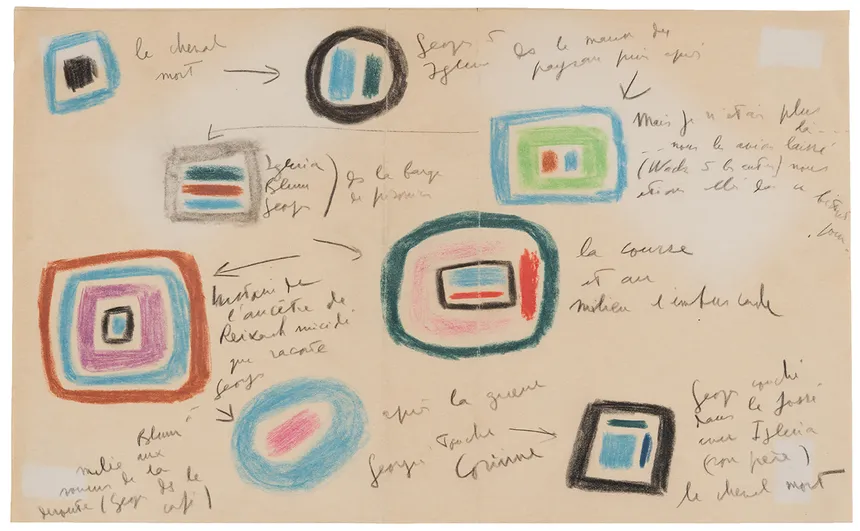
\includegraphics[width=\textwidth,height=\textheight,keepaspectratio]{routedesflandres.png}
    \caption{Tentative d'organisation visuelle pour le roman La Route des Flandres, années 1960 - Claude Simon, écrivain}
    \label{graphic:routedesflandres}
\end{figure}

Going beyond logical notation, we have seen that there are other conceptions of knowledge which take into account the physical, social and linguistic context of an action. Nonetheless, these can still be systematized, as Goodman highlights in his investagation of referential systems, with a focus on reference of the ideas at hand.

\subsubsection{Constructing knowledge}
\label{subsubsec:constructing-knowledge}

There are multiple ways to express an idea: on can use formal notation or draft a rough sketch with different colors. These all highlight different degrees of expression, but one particular way can be considered problematic in its ambition. Formal languages rely on the assumption, that all which can be known can ultimately be expressed in unambiguous terms. First shown by Wittgenstein in the two main eras various eras of his work, we know focus on the ways of knowing which cannot be explicited.

First of all, there is a separation between \emph{knowing-how} and \emph{knowing-that}; the latter, propositional knowledge, does not cover the former, practical knowledge, as shown by Ryle \citep{ryle_concept_1951}. Perhaps one of the most obvious example of this duality is in the failure of Leibniz to construct a calculating machine, as told by Matthew L. Jones in his book \emph{Reckoning with Matter}. In it, he traces the history of philosophers to solve the problem of constructing a calculating machine, a problem which would ultimately be solved by Charles Babbage, with the consequences that we know \citep{jones_reckoning_2016}.

Jones depicts Leibniz in his written correspondence with watchmaker Ollivier, in their fruitless attempt to construct Leibniz's design; the implementations details seem to elude the German philosopher as he refers to the "confused" knowledge of the nonetheless highly-skilled Parisian watchmaker. The (theoretical) plans of Leibniz do not match the (concrete) plans of Ollivier.

These are two complementary approaches to the knoweldge of something: to know \emph{what} constructing calculating machine entails and knowing \emph{how} to construct such a machne. In the fact that Ollivier could not communicate clearly to Leibniz what his technical difficulties, we can see an instance of something which would be theorized centuries later by Michael Polanyi as \emph{tacit knowledge}, knowledge which cannot be entirely made explicit.

Polanyi, as a scientist himself, starts from another assumption: we know more than we can tell. In his eponymous work, he argues against a positivist approach to knowledge, in which empirical and factual deductions are sufficient to achieve satisfying epistemological work. What he proposes, derived from \emph{gestalt} psychology, is to consider some knowledge of an object as the knowledge of an integrated set of particulars, of which we already know some features, by virtue of the object existing in an external approach. This integrated set, in turn, displays more properties than the sum of its parts. While formal notation suggests that the combination of formal symbols does not result in additional knowledge, Polanyi rather argues, against Descartes, that relations and perceptions do result in additional knowledge.

\begin{quote}
    The knowledge of a problem is, therefore, like the knowing of unspecifiables, a knowing of more than you can tell. \citep{polanyi_knowing_1969}
\end{quote}

Rooted in psychology, and therefore in the assumption of the embodimed of the human mind, Polanyi posits that all thought is incarnate, that it lives by the body and by the favour of society, hence giving it a physio-social dimension. This confrontation with the real-world, rather than being a strict hurdle that has to be avoided or overcome, as in the case of SHRDLU above, becomes one of the two poles of cognitive action. Knowledge finds its roots and evaluation in concrete situations, as much as in abstract thinking. In the words of Cecil Wright Mills, writing about his practice as a social scientist research,

\begin{quote}
    Thinking is a continuous struggle between conceptual order and empirical comprehensiveness. \citep{MillsC.WrightCharlesWright2000Tsi}
\end{quote}

Polanyi's presentation of a form of knowledge following the movement of a pendulum, between dismemberment and integration of concepts finds an echo in the sociological work of Mills: a knowledge of some objects in the world happens not exclusively through formal descriptions in logical symbol systems, but involves imagination and phenomenological experience—wondering and seeing. This reliance on vision—starting by recognizing shapes, as Polanyi states—directly implies the notion of aesthetic assessment, such as a judgement of typical or non-typical shapes. He does not, however, immediately elucidate how aesthetics support the formation of mental models at the basis of understanding, only that this morphology is at the basis of higher order of represenations.

Seeing, though, is not passive seeing, simply noticing. It is an active engagement with what is being seen. Mills's quote above also contains this other aspect of Polanyi's investigation of knowledge, and already present in Ollivier's relation with Leibniz: knowing through doing.

This approach has been touched upon from a practical programmer's perspective in section \ref{subsec:craft-knowledge}, through a historical lens but it does also posses theoretical grounding. Specifically, Harry Collins offers a deconstruction of the Polanyi's notion by breaking it down into \emph{relational}, \emph{somatic} and \emph{collective} tacit knowledges \citep{collins_tacit_2010}. While he lays out a strong approach to tacitness of knowledge (i.e. it cannot be communicated at all), his distinction between relational and somatic is useful here\footnote{His definition of collective tacit knowledge touches on the knowledge present in any living species and is impossible to ever be explicited, and is therefore out of scope here.}. It is possible to think about knowledge as a social construct, acquired through social relations: learning the linguo of a particular technical domain, exchanging with peers at conferences, imitating an expert or explaining to a novice. Collective, unspoken agreements and implicit statements of folk wisdom, or implicit demonstrations of expert action are all means of communication through which knowledge gets replicated across subjects.

Concurrently, somatic tacit knowledge tackles the physiological perspective as already pointed out by Polanyi. Rather than knowledge that exists in one's interactions with others, somatic tacit knowledge exists within one's physical perceptions and actions. For instance, one might base one's typing of one's password strictly on one's muscle memory, without thinking about the actual letters being typed, through repetition of the task. Or one might be spotting a cache bug which simply requires a machine reboot, due to experience machine lifecycles, package updates, networking behaviour. Not completely distinct from its relational pendant, somatic knowledge is acquired through experience, repetition and mimeomorphism—replicating actions and behaviours, or the instructions, often under the guidance of someone more experienced.

\spacer

We started our discussion of understanding by defining it as the acquisition of the knowledge of a object—be it a concept, a situation, an individual or an artfefact,, which is accurate enough that it allows us to predict the behaviour and to interact with such object. Within this defintion, one could take the example of a human discussion as a demonstration of advanced understanding, as something that is both situated, and formalized.

Theories of how individuals acquire understanding (how they come to know things, and know conceptual representations of things), have been approached from an explicit perspective, and an implicit one. In the rationalist, logical philosophical tradition, we have seen that the belief that meaning can be rendered unambiguous through the use of specific notation. This has led to the development of logic and computer science, as this meaning got mechanized. Explicit understanding is therefore the theoretical lineage of computation.

However, as we have seen in the first hurdles of artificial intelligence research, explicit specification of meaning falls short of handling everyday tasks which humans would consider to be menial. This has led us to consider a more implicit approach to understanding, in which it is acquired by tacit means. Particularly, we have identified this tacit knowledge as relying on a social component, as well as on a somatic component.

Source code, as a formal system with a high dependence of context, intent and implementation, mobilizes both approaches to understanding. Before we dive deeper about how these two modes of understanding are mobilized at the end of this chapter, we now turn to what makes computation a cognitively complex object, and what are some cognitive reactions that humans display in situations where they have to understand, and work with, software.

\clearpage

\section{Understanding computation}
\label{sec:understanding-computation}

In the previous chapter, we have laid out the groundwork by showing that there are multiple ways to understand something. We now turn to the thing we want to understand. What makes it challenging to understand computation?

First, we will inquire into some distinguishing features of software in terms of levels of abstractions, and in terms of types of complexity. This will highlight some of the theoretical properties that make it hard to understand, such as its relation to hardware, its relation to a specification, and its relation to time and space.

Then, we will shift our perspective to a more abstract point of view, investigating the ontological status of software. This will highlight how software exists as an \emph{abstract artifact}, simultaneously on the ideal, practical and physical plane.

Finally, we will conclude this section by looking specifically at the source code component of software, and how programmers deploy strategies to understand it. Approaching it from a cognitive and psychological perspective, this will give us a better picture of the concrete process of understanding source code—a process which aesthetics are primarily intended to affect.

% the software effect (combination of knowing what (it does) and how (it does it))
\subsection{Software complexity}
\label{subsec:software-complexity}

Software exhibits several particularities, which result in a compex whole—meaning that software possesses several independent components which interact with each other in non-trivial, and non-obvious ways. This subsection focuses on these particularies; that is, on the \emph{properties} of software, and hence how these properties manifest themselves concretely, leading to those complex interactions. We will start by looking at the different levels at which software exists, before turning to the different kinds of complexity which make software hard to grasp.

\subsubsection{Levels of software}
\label{subsubsec:levels-software}

One of the essential aspects of software is that of \emph{implementation}. Implementation is the realization of a plan, the concrete manifestation of an idea, and therefore hints at a first tension in software's multiple facets. It can happen through individuation, instantation, exemplification and reduction \citep{rapaport_philosophy_2005}. On the one side, there is what we will call here \emph{ideal} software, often existing only as a shared mental representation by humans (not limited to programmers), or as printed documentation, as a series of specifications, etc. On the other side, we have \emph{actual} software, which is manifested into lines of code, written in one or more particular languages, and running with more or less bugs.

The relationship between the \emph{ideal} and the \emph{actual} versions of the same software is not straightforward. Ideal software only provides an intent, a guidance towards a goal, assuming, but not guaranteeing, that this goal will be reached. A popular engineering saying is that complements this approach by stating that:

\begin{quote}
    In theory, there is no difference between theory and practice. In practice, there is.\footnote{Sometimes mis-attributed to Richard P. Feynman or Albert Einstein, but traced to Benjamin Brewster, writing in the Yale Literary Magazine of 1882.}
\end{quote}

Actual software, as most programmers know, differs greatly from its ideal version, largely due to the process of implementation, translating the purpose of the software from natural and diagrammatic languages, into programming languages, from what it should do, into what it actually does.

Writing on the myths of computer science, James Moor \citep{moor_three_1978} allows us to think through this distinction between ideal and practical along the lines of the separation between a theory and a model. The difference between a model and a theory is that both can exist independently of one another—one can have a theory for a system without being able to model it, while one can also model a system using \emph{ad hoc} programming techniques, instead of a coherent theory.

Most of the practice of programmers (writing and reading code for the purposes of creating, maintaining and learning software) depends on closing this gap between the ideal and the practical existences of software.

The third level at which software exists is that of hardware. While the ideal version of software is presented in natural language, diagrams or pseudo-code, and while the practical version of software exists as executable source code, software also exists at a very physical level—that of transistors and integrated circuits.

The distinction between software and hardware has been examined thoroughly \citep{kittler_there_1997,chun_sourcery_2008,rapaport_philosophy_2005}, but never strictly defined. Rather, the distinction between what is hardware and what is software is relative to where one draws the line: to a front-end web developer writing JavaScript, the browser, operating system and motherboard might all be considered hardware. For a RISC-V assembly programmer, only the specific CPU chip might be considered hardware, while the operating system being implemented in C, itself compiled through Assembly, would be considered software. A common definition of hardware, as the physical elements making up the computer system, overlooks the fact that software itself is, ultimately, physical changes in the electrical charge of the components of the computer.

Software can be characterized the dynamic evolution of logical processes, described as an ideal specification in natural languages, as a practical realization in programming languages, and in specific states of hardware components. Furthermore, the relations between each of these levels is not straightforward: the ideal and the practical can exist independently of each other, while the practical cannot exist independently of a machine\footnote{Even if that machine is a \emph{virtual machine}, further complicating the boundary between hardware and software}.

\subsubsection{Types of complexity}
\label{subsubsec:types-complexity}

Along with different levels of existence needed to be taken into account by the programmer, software also exhibits specific kinds of complexity. Our definition of complexity will be the one proposed by Warren Weaver. He defines problems of (organized) complexity as those which involve dealing simultaneously with a sizable number of factors which are interrelated into an organic whole \citep{weaver_science_1948}\footnote{As opposed to disorganized complexity, which are dealt with statistical tools.}. Specifically, there are four different types of software complexity that we look at: conceptual complexity, modeling complexity, temporal complexity and spatial complexity.

Conceptual complexity, as refered to by Lando et. al. in their ontology of computer programs, addresses the necessity to model complex objects at different abstraction levels \citep{lando_general_2007}. As mentioned above, software exists at least on three somewhat distinct levels: the ideal, the practical, and the physical. This means that software, in its source code representation, should be able to provide the programmer with tools to engage with its intended function and its actual function at each of these levels. For instance, comments might relate to the ideal behaviour of the software, function declarations to its practical behaviour, while macro definitions can point to the specific hardware on which the code is run.

% insert a table of C code where you see some comment, some function, and some macro

Additionally, conceptual complexity involves the distinction of the different elements of a computer program at the source code level, and keep track of their ontological status, sometimes independently from its level of existence. This distinction should be made notwithstanding the naming conventions assigned by different platforms, vendors, or programming languages, and rather based on ontological properties of the elements at hand. For instance, the distinction between \emph{endurants} and \emph{perdurants} by Lando et. al. focuses on the temporal dimension of software components (i.e. a data structure declaration has a different temporal property than a function call). Here we have a second, complementary frame to that of the levels of existence, through which we can analyze source code; being somewhat related but an exact mapping of one another.

Modeling complexity addresses the hurdles in translating a non-discrete, non-logical object, event, or action, into a discreete, logical software description through source code. Indeed, the history of software development is also the history of the extension of the application of software, and the hurdles to be overcome in the process. From translation of natural languages \citep{poibeau_machine_2017}, to education \citep{watters_teaching_2021} or psychological treatment \citep{weizenbaum_computer_1976}, it seems that problems that seem somehat straightforward from a human perspective become more intricate once the time for implementation has come.

we have seen so far the complexities tied to the conceptualization and modelization of the components of software. Two other significant contributions to the cognitive load of understanding software happen are more closely related to the concrete execution of the software—temporal and spatial complexity.

Temporal complexity relates to the discrepancy between the way the computer was first thought of —i.e. as a Turing machine which operates linearly, on a one-dimensional tape—and further technological developments. Originally, the Turing machine would involve the ability for the head of the machine to jump at different locations. This meant that the execution and reading of a program would be non-linear, jumping from one routine to another across the source code. Such an entanglement is particulary obvious in Ben Fry's Distellamap series of visualizations of source code (\ref{graphic:pacman-visualization} represents the execution of the source code for the arcade game Pac-Man), and led to Edsger W. Dijkstra's statement on the harmfulness of such jumps on the cognitive abilities of programmers.


\begin{figure}
    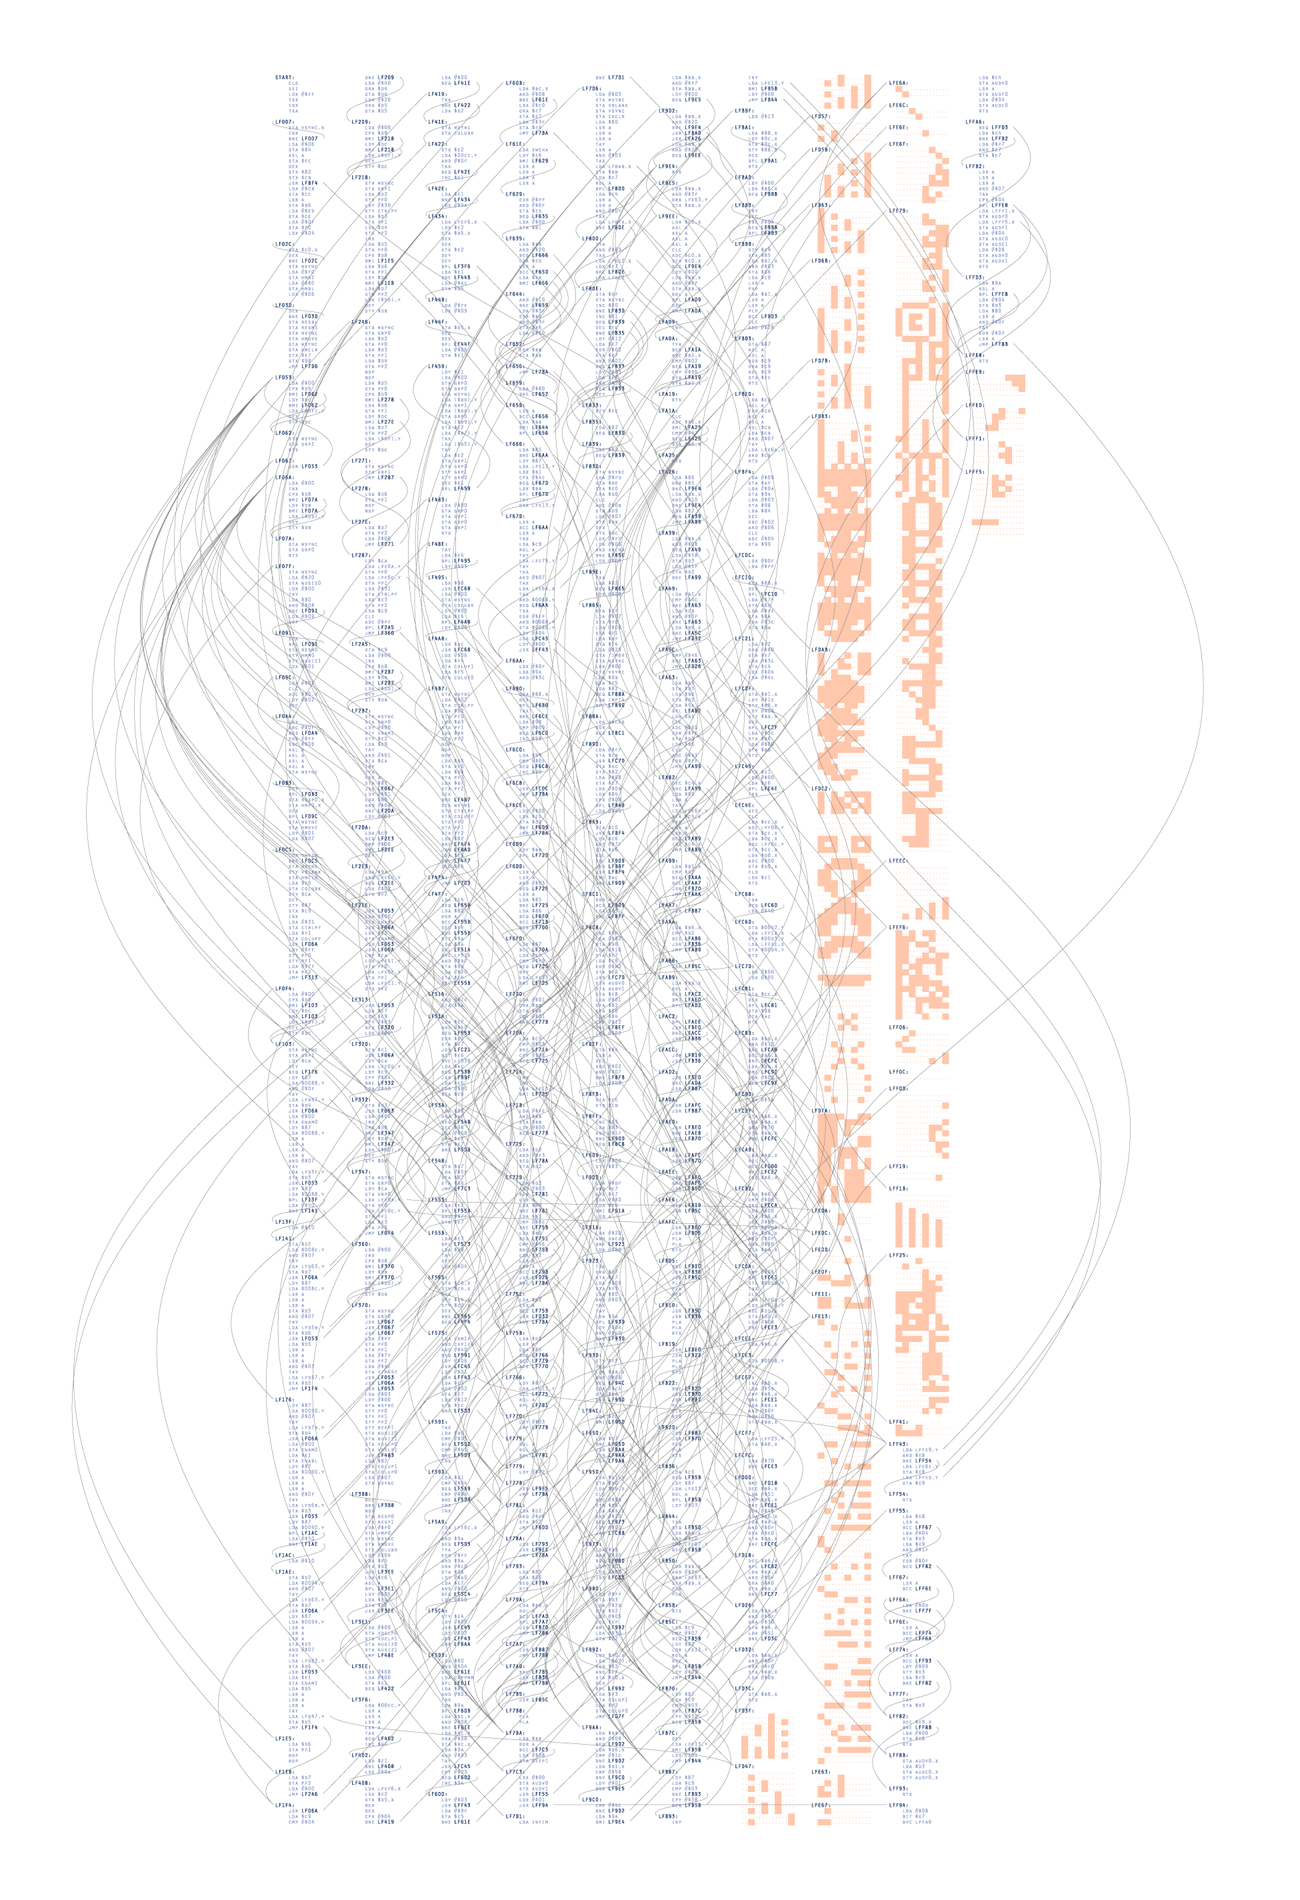
\includegraphics[width=\textwidth,height=\textheight,keepaspectratio]{distellamap_pacman.png}
    \caption{Visualization of the execution of Pac-Man's source code}
    \label{graphic:pacman-visualization}
\end{figure}

Later on, the introduction of multi-core architecture for central processing units in the late 2000s has enabled the broad adoption of multithreading and threaded programming. As a result, source code has transformed from a single non-linear execution to a multiple non-linear process, in which several of these non-linear executions are happening in parallel. Keep tracking of what is executing when on which resource is involved in problems such as \emph{race conditions}, when understanding the scheduling of events (each event every e.g. 1/18000000th of a second on a 3.0 Ghz CPU machine) becomes crucial to ensuring the correct behaviour of the software.

Conversely, the locii of the execution of software creates contributes to those issues. Software can be (dis-)located across multiple files on a single machine, on multiple processes on a single machine, or on multiple processes on multiple machines (on a local-area or wide-area network) \citep{berry_philosophy_2011}. This further fragments the interface to the object of understanding. For instance, the asynchronicity of requesting and processing information from distinct processes is a spatial separation of code which has temporal implications (e.g. due to network latency).

\spacer

Software, then, exhibits certain properties which make it difficult to understand, from conception to application: software in the real-world involves implementing concepts that lose in translation, interfacing the world through discreete representations, and following the execution of these representations through space and time, as software executes more and more in a distributed and parallel fashion.

% the philosophical enquiries
\subsection{Software ontology}
\label{subsec:software-ontology}

Now that we have clarified some of what software complexity consists of, we will frame these difficulties in a philosophical context, more specifically the philosophy of technology. We will investigate how these complexities can be seen as stemming from the nature of technology itself, and how this allows us to reconnect it to aesthetic perception. Before moving back to practical inquiries into how specific individuals engage with this nature, this section will help provide a theoretical backdrop, framing technology as a relational practice, complementing other modes of making sense of and taking action on the world. This conceptual framework will start with an investigation into the denomination of software as an \emph{abstract artifact}, followed by an analysis of technology as a specific mode of being, and concluding on how it is related to an aesthetic mode of being.

\subsubsection{Software as abstract artifact}
\label{subsubsec:abstract-artifact}

When he coins the phrase \emph{abstract artifact}, Nurbay Irmak addresses software partly as an abstract object, similar in his sense to Platonic entities\footnote{Like Joseph Kosuth's aforementioned trio of chairs..}. Nonetheless, he also grants that software holds spatio-temporal properties \citep{irmak_software_2012}. Indeed, software does need to exist as an implementation, in the form of source code \citep{suber_what_1988}; this implies that software is composed of files, has a beginning (start) and an end (exit), meanwhile also representing ideas of structure and procedure which go beyond these limitations of being written to a disk and having an execution time. Typically, the physical aspects of software (its manifestation as source code) can be changed\footnote{A process called \emph{refactoring}.} without changing any of the ideas expressed by the software\footnote{A phenomenon one can also observe in natural languages, in which one can radically change a syntax without drastically changing the semantics of a sentence.}.

Complementing Irmak, Colburn's phrasing is that of a \emph{concrete abstraction}, an oxymoron which echoes the tensions denoted by the concept of an abstract artifact.

He grounds these tensions in the distinction between a medium of execution (a—potentially virtual—machine) and a medium of description (source code). He considers that, while any high-level programming language is already the result of layers of abstraction, such language gets reduced to the zeroes and ones input to the central processing unit \citep{colburn_philosophy_2000}. Here, he sees the abstraction provided by languages ultimately bound to the concrete state of being of hardware and binary. And yet, if we follow along along his reasoning, these representations of voltage changes into zeroes and ones are themselves abstractions over yet another concrete, physical event.

Writing on computational artefacts, of which software is a subset, Raymond Turner formalizes this specificity of in a three-way relationship. Namely, abstract artefact A is an implementation in medium M of the definition F. For instance, concerning the medium:

\begin{quote}
    Instead of properties such as \emph{made from carbon fiber}, we have properties such as \emph{constructed from arrays in the Pascal programming language, implemented in Java}. \citep{turner_computational_2018}
\end{quote}

This metaphor provides an accurate but limited account of the place of source code within the definition of software: the Java implementation is itself a definition implemented in a specific bytecode, etc. Nonetheless, source code is that which gives shape to the ideas immanent in software—through a process of concretization—and which hides away the details of the hardware—through abstraction. This metaphor of \emph{abstract artifact} thus helps to clarify the tensions within software, and to locate the specific role of source code within the different moving parts of definition, medium and model.

Recalling that software has a somewhat unique relatoin between its \emph{functional} properties (i.e. purpose that are intended to be achieved through their use) and \emph{structural} ones (physical configuration which are involved in the fullfilment of the functional purpose) \citep{turner_computational_2018}, it remains nonetheless a kind of technology. As such, it also holds some of the specifities of this lineage, into which we can extend our inquiry.

\subsubsection{Software as a relational object}
\label{subsubsec:software-relational}

The technological object underwent a first qualitative shift during the European Industrial Revolution, and a second one with the advent of computing technologies. The status of its exact nature is therefore a recent object of inquiry. Here, we will start from Gilbert Simondon's understanding of technology as a \emph{mode}, in order to ultimately contrast it with the \emph{aesthetic mode}.

According to Simondon, the technical object is a relation between multiple structures and the result of a complex operation of various knowledges \citep{simondon_mode_1958}, some scientific, some practical, some social, some material. The technical object is indeed a scientific object, but also a social object and an artistic object at the same time. Differentiated in its various stages (object, individual, system), it is therefore considered as relational, in that its nature changes through its dependance and influence on its environment.

From this relational standpoint, one could complement Bernard Stiegler's statement that technology is a dynamic of organized, but inorganic matter \citep{stiegler_technics_1998}, if we are to consider inorganized matter to include social influences, personal practices, and forms of tacit and explicit knowledges. That is, the ambiguity of the technical object is that it extends beyond itself as an object, entering into a relation with its surrounding environment, including the human individual which makes use of it. Up until the invention of the clock, technology remained bound to practical matter. With the invention of seconds, its action reached into another domain—that of mechanical operation on abstract ideas \citep{mumford_technics_1934}.

The domain of abstract ideas was hitherto reserved to different modes than technology: that of religion and philosophy, and technology holds a particularly interesting relation with these two. According to Simondon, philosophy followed religion as a means of relating to, and making sense of, the abstract such the divine and the ethical. Tracing back the genesis of the technological object, e writes that the technical mode of existence is therefore just another mode through which the human can relate to the world, similar to the religious, the philosophical, and the aesthetic mode\citep{simondon_mode_1958}.

While both technology, religion and philosophy are based on theoretical knowledge, technology is specifically manifested in practice, and while it is manifested in ethics, in religion. Technology is thus seen as the combination of a theory of knowledge and a theory of action. Such a combination has since been extended into the abstract domain, leading to computers, as a form of technology through which \emph{meaning is mechanically realized}.

%TODO add a section on yuk hui here, for the digital objects.

Simondon complements the technical and the religious modes with the aesthetic mode, and as such counter-balances the apparent split between technics and religion by striving for unity and totality, for the balance between the objective and the subjective. Yet, rather than being a monadic unity of a single principle, Simondon considers the aesthetic mode as a unifying a network of relationships, a form of organizing Stiegler's inorganized matter. He further argues that the aesthetic mode goes beyond taste and subjective preference, into a fundamental aspect of the way in which human beings relate to the world around them. An aesthetic object therefore acquires the property of being beautiful by virtue of its relationships, of its connections between the subject and the objective, between one's history and one's perceptions, and the various elements of the world, and the actions of the individual. Finally, the aesthetic thought when related to the technical object consists in preparing the communication between different communities of users, between different perspectives on the world, and different modes of action upon this world. An aesthetic object can therefore be seen as a nexus of relationships found in its environment, echoing how Goodman considers an aesthetic language as way for worldmaking.

Software is therefore a manifestation of technology as both knowledge and action. Furthermore, it also enables ways to act mechanically on knowledge and ideas, an affordance named \emph{epistemic action} by David Kirsh and Paul Maglio \citep{kirsh_distinguishing_1994}. They define epistemic actions as actions which facilitate thinking through a particular situation or environment, rather than having an immediate functional effect on the state of the world. As technology changes the individual's relationship to the world, software does so by being the dynamic notion of a state of a process \citep{rapaport_philosophy_2005}, ever evolving around a fixed structure, and by changing the conceptual understanding of said world. Such examples of world related to the environment in which software exists, e.g. the social environment, or hardware environment, or the environment which has been recreated within software. David M. Berry investigates this encapsulation of world in his \emph{Philosophy of Software}:

\begin{quote}
    The computational device is, in some senses, a container of a universe (as a digital space) which is itself a container for the basic primordial structures which allow further complexification and abstraction towards a notion of world presented to the user. \citep{berry_philosophy_2011}
\end{quote}

Software-as-world is the material implementation of a proposed model, itself derived from a theory. It therefore primarily acts at the level of \emph{episteme}, sometimes even limiting itself to it\footnote{Functional programming languages take pride in the fact that they have no effect on the world around them, being composed exclusively of so-called \emph{pure functions}, and no external side-effects, or input/output considerations}. Paradoxically, it is only through peripherals that software can act as a mechanical technology in the industrial sense of the word.

Along with software's material and theoretical natures (i.e. in contemporary digital computers, it consists of electrons, copper and silicium and of logical notations), another environment remains—that of the intent of the humans programming such software. Since it can be so many things, it might not be exactly clear what a specific piece of software, manifested in source code, is exactly about.

Indeed, thinking through the function of computational artefacts, Turner states that it is \emph{agency} which determines what the function is: and he defines agency as the resolution of the difference between the specification (intent-free, external to the program) and semantic interpretation (intent-rich, internal to the programmer) \citep{turner_computational_2018}. In order to understand a computer program, to understand how it exists in mutliple worlds, and how it represents the world, we need to give it meaning. To make sense of it, a certain amount of interpretation is requiredin relation to that of the computer's—such that the question "what does a Turing machine do?" has \lstinline{n+1} answers. 1 syntactic, and \lstinline{n} semantic (e.g. however many interpretations as there can be human interpreters) \citep{rapaport_philosophy_2005}. In his investigation into what software is, Suber corroborates:

\begin{quote}
    This suggests that, to understand software, we must understand intentions, purposes, goals, or will, which enlarges the problem far more than we originally anticipated. [\dots] We should not be surprised if human compositions that are meant to make machines do useful work should require us to posit and understand human purposiveness. After all, to distinguish \emph{literature} from noise requires a similar undertaking. \citep{suber_what_1988}
\end{quote}

\spacer

In conclusion, we have seen that while software can be given the particular status of an \emph{abstract artifact}, these tensions are shared across technological objects. Technology, as a combination of a theory of knowledge and a theory of action, as an interface to the world and a recreation of the world, is furthermore related to other modes of existence—and in particular the aesthetic mode. All of these tensions and paradoxes, from the various levels of existence, the various types of complexities, the different kinds of actions and interpretations that it allows, contribute to the cognitive hurdles encountered when attempting to understanding software.

And yet, programmers, have been understanding software as long as they have been writing and reading it. We now turn to understanding how programmers understand software, through a empirical perspective of the psychology of programming..

\subsection{The psychology of programming}
\label{subsec:psychology-programming}

How programmers deal with such a complex object as software has been a research topic which appeared much later than software itself. This field aims at understanding how programmers process code, and with which level of success, and under which conditions. How do they build up their understanding(s), in order to afford appropriate modification, re-use or maintenance of the software? What cognitive abilities do they summon, and what kind of technical apparatuses play a role in this process? Specifically, we will see how hard it is to answer these questions, and how diversity and multiplicity are recurrent patterns in sketching out answers.

Epistemic actions thus contribute to reducing the kinds of complexities involved with software. Concretely, this involves the creation of mental models of the software system with which the indvidual is interacting. In their work on computer-enabled cognitive skills, Kirsh and Maglio develop on the use of epistemic actions:

\begin{quote}
    More precisely, we use the term epistemic action to designate a physical action whose primary function is to improve cognition by:
    \begin{enumerate}
        \item{reducing the memory involved in mental computation, that is, space complexity;}
        \item{reducing the number of steps involved in mental computation, that is, time complexity;}
        \item{reducing the probability of error of mental computation, that is, unreliability.}
    \end{enumerate}
    \citep{kirsh_distinguishing_1994}
\end{quote}

Psychological studies of programming practices have been focused on the identification and analysis of these mental models, as well as on their optimization through experimental devices, and the social behaviour of programmers within a context of practice \citep{weinberg_psychology_1998}.

Mental models, as kinds of internal symbolic representation of an external reality, are a rigorous, personal and conceptual structure. They are related to knowledge, since the construction of accurate and useful mental models through the process of understanding underpins knowledge acquisition. However, mental models need not be correlated with empirical truth, due to their personal nature, but are extensive enough to be described by formal (logical or diagrammatical) means. Mental models can be informed, constructed or further qualified by the use of metaphors, but they are nonetheless more precise than other cognitive structures such as metaphors—a mental model can be seen as a more specific instance of a conceptual structure.

The earliest studies of how computer programmers understand the code they are presented with consisted mostly in pointing out the methodological difficulties in doing so \citep{sheil_psychological_1981,shneiderman_measuring_1977}. This is mainly due to three parameters. First, programming is an intertwined combination of notation, practices, tasks and management, each of which have their own impact on the extent to which a piece of source code is correctly understood, that it is hard to clearly establish the impact of each of these. Second, program comprehension is strongly influenced by practice—the skill level of the programmer therefore also influences experimental conditions. Third, these early studies have found that programmers have organized knowledge bases, if informal. This means that, while programmers demonstrate epistemic mastery, they are limited in their ability to explain the workings of such ability—that is, the constitution and use of their own epistemic models, which she calls knowledge maps.

Shifting to qualitative interviews, rather than quantitative and performative assessments, Marian Petre and Alan Blackwell attempted in their 1992 study to identify these mental models and their uses. They asked 10 expert programmers from North America and Europe to describe the thought process in source code-related problem-solving and design solutions in code. The main conclusion of their study is that, beyond the fact that each programmer had slightly different descriptions of their mental process, there a some commonalities to what is happening in someone's thoughts as they start to design software. The behaviour is dynamic, but controlled; the resolution of that behaviour was also dynamic, with some aspects coming in and out of focus that the will of the programmer, providing more or less uncertainty, level of details and fuzziness on-demand; and those images co-existed with other images, such that one representation could be compared with another representation of a different nature \citep{petre_glimpse_1997}. Finally, while most imagery was non-verbal, all programmers talked about the need to have elements of this imagery labelled at all times, hinting at a relationship between syntax and semantics to be translated into source code. While this study was an investigation into the design of code, before any writing happens, one of the limitations is that it did not investigate the understanding of code, which takes places once the writing has been done (by oneself, or someone else), and the code now needs to be read.

Francoise Détienne, in her study of how computer programmers design and understand programs \citep{detienne_software_2012}, defines the activity of designing and understanding programs in activating \emph{schemas}, mental representations that are abstract enough to encompass a wide use (web servers all share a common schema in terms of dealing with requests and responses), but nonetheless specific enough to be useful (requests and responses are qualitatively different subsets of the broader concept of inputs and outputs). An added complexity to the task of programming comes with the one of the dual nature of the mental models needing to be activated: the computer's actions and responses are comprised of the prescriptive (what the computer should do) to the effective (what the computer actually does). In order to be appropriately dealt with, then, programmers must activate and refine mental models of a program which resolves this tension.

In programming, within a given context—which includes goals and heuristics—, elements are being perceived, processed through existing knowledge schemas in order to extract meaning. Starting from Kintsch and Van Dijk's approach of understanding text \citep{kintsch_model_1978}, Détienne nonetheless highlights some differences with natural language understanding. In program texts, she finds, there is an entanglement of the plan, of the arc, of the tension, which does not happen so often in most of the traditional narrative text. A programmer can jump between lines and files in a non-linear, explorative manner, following the features of computation, rather than textuality. Program texts are also dynamic, procedural texts, which exhibit complex causal relations between states and events, which need to be kept track of in order to resolve the prescriptive/effective discrepancies. Finally, the understanding of program text is first a general one, which only subsequently applies to a particular situation (a fix or an extension needing to be written), while narrative texts tend to focus on specific instances of protagonists, scenes and descriptions, leading to broad thematic appreciation.

Conversely, a similarity in understanding program texts and narrative texts is that the sources of information for understanding either are: the text itself, the individual experience and the broader environment in which the text is located (e.g. technical, social). Building on Chomsky's concepts, the activity of understanding in programming can be seen as understanding the \emph{deep structure} of a text through its \emph{surface structure} \citep{chomsky_aspects_1965}. One of the heuristics deployed to achieve such a goal is looking out for what she calls \emph{beacons}, as thematic organizers which structure the reading and understanding process. For instance, in traditional narrative texts, beacons might be represented by section headings, or the beginning or end of paragraphs. However, one of the questions that her study hasn't answered specificall, how the specific surface structure in programming results in the understanding of the deep structure—in other terms, what is the connection between source code syntax, programmer semantics and program behavior.

Due to its relation to text, syntax and semantics, it has often been assumed by programmers and researchers that reading and writing code is akin to reading and writing natural languag prose. Additional recent research in the cognitive responses to programming tasks, conducted by Ivanova et. al., do not appear to settle the question of whether programming is rather dependent on language processing brain functions, or on functions related to mathematics (which do not rely on the language part of the brain) \citep{ivanova_comprehension_2020}, but contributes empirical evidence to that debate. They conclude that, while language processing might not be one of the essential ways that we process code—excluding the \emph{code is language} hypothesis—, it also does not rely on exclusively mathematical functions. Stimulating in particular the so-called multi-demand system, it seems that programming is a polymorphous activity involving multiple exchanges between different brain functions. What this implies, though, is that neither literature, linguistics nor mathematics should be the only lens through which we look at code.

In a way, then, programming is a sort of fiction, in that the pinpointing of its source of existence is difficult, and in that it affords the experience of imagining contents of which one is not the source, and of which the certainty of isn't defined. Both programming and fiction suggest surface-level guiding points helping the process of constructing mental models as a sort of conceptual representation. It is also something else than fiction, in that it deals with concrete issues and rational problems \footnote{more often than not, a pestering bug}, and that it provides a pragmatic frame for processing representations, in which assumptions stemming from burgeoning mental models can be easily verified or falsified, through the taking of epistemic actions. It might then be appropriate to treat it as such, simultaneously fiction and non-fiction, as knowledge and action, mathetmatic and artistic. Indeed, it is also an artistic activity which, in Goodman's terms, might be seen as \emph{an analysis of [artistic] behavior as a sequence of problem-solving and planning activities."} \citep{goodman_basic_1972}.

Remains the interpretation issue mentioned above: the interpretation of the machine is different from the interpretation of the human, of which there are many, and therefore what also needs to be intepreted is the intent of the author(s). Reading is then akin to constructing a \emph{cognitive cartography}, allowing for an experience to be made intelligible, sensible, and verifiable, and when an experience is made sensible is when it enters the realm of the aesthetic. In a very immediate understanding of aesthetics, we conclude on the role of form in cognition in those psychological studies. One of the focus was on demonstrating the impact that formal arrangement has on program comprehension\citep{oman_typographic_1990,oliveira_systematic_2022}. Spacing, alignment, syntax highlighting and casing are all parameters which have an impact on the readability, and therefore understandability of code. The next section therefore looks at two ways in which meaning can be extracted from intention and source code; this means how individuals use metaphors to communicate complex ideas, and how they use computational tools in order to navigate program texts.

%todo include comparison of color vs. not color coded (or maybe in the IDE section below?)

The fact that software exists between the state of being conceptually designed and materially implemented predates software itself, and can be observed in modern technological developments at large. Furthermore, these complexities are echoed in how programmers evoke their experience of either designing or, comprehending code. They have shown to use multiple cognitive abilities, without being strictly limited to narrative, or mathematic frames of understanding, and making use of notions of scale and focus to disentangle complexity. For the remaining section of this chapter, we will focus on two specific means that contribute to this process of building a mental model of software-as-source code. Based on the reports that programmers use mental images and play with dynamic mental structures to comprehend the functional and structural properties of software; we thus inquire into the role that metaphors play in translating computational concepts into ones which can be grasped by an individual. Conversely, in response to the role of indentation, typography and navigation, we will see how cognition is also distributed in a programmers' tools.

\clearpage

\section{Means of understanding}
\label{sec:means-understanding}

Drawing on the ambivalence of software's existence—both concrete and abstract—we now investigate the means deployed to graps software on both of these levels. As we have seen in empirical studies, programmers resort to both conceptual techniques to visualize and grasp a piece of software, along with more practical and technical tools. In this spirit, we will look at the ubiquity of metaphors in computing,  both from users and programmers, and how they act as a cognitive mechanism. We will also look at how cognitive tools can be manifested concretely though the extension of mind through software tools, and particularly on the role of \emph{Integrated Development Environments} (IDEs). This will establish the research ground of the subsequent chapters, in which we establish aesthetics as one of the cognitive tools used by programmers.

\subsection{Metaphors in computation}
\label{subsec:metaphor-computation}

This part of the thesis relies on the work of George Lakoff and Mark Johnson, and on that of Paul Ricoeur, due to their requalification of the nature and role of metaphor in the 20th century. While Lakoff and Johnson's approach to the conceptual metaphor will serve a basis to explore metaphors in as a cognitive means across software and narrative, I also argue that Ricoeur's focus on the tension of the \emph{statement} rather than primarily on the \emph{word} will help us better understand some of the aesthetic manifestations and workings of software metaphors. Following a brief overview of their contributions, I examine the various uses of metaphor in software.

\subsubsection{Theoretical background}
\label{subsubsec:metaphors-background}

%and in literature, touch upon the cognitive turn in literary studies, and conclude the section by the ambiguity of a cognitive account of programming.

We depart here from the most commonly used definition of metaphor: that of labeling one thing in terms of another, thereby granting additional meaning to the subject at hand. Our approach here will also bypass some of the more minute distinctions made between metonymy (in which the two things mentioned are already conceptually closely related), comparison (explicitly assessing differences and similarities between two things, often from a value-based perspective) and synechdoche (representing a whole by a subset), as they all relate to a larger, more contemporary definition of the concept.

Such a definition stems from Lakoff and Johsnon's seminal work through which they develop a theory of conceptual metaphors by highlighting their essential dependence on pre-existing cognitive structures, which we associate with already-understood concepts. The metaphor maps a source domain (made up of cognitive structure(s)) to a target domain. In the process, they extend the field of applicability of metaphors from the strictly literary to the broadly cultural: metaphors work because each of us has some conception of those domains involved in the metaphorical process. Metaphors rely in part on a static understanding, resulting in a fixed meaning from the application of a given source to a given target. Some of these sources are called \emph{schemas}, and are defined enough to not be mistaken for something else, but broad enough to allow for multiple variants of itself to be applied to various targets \citep{lakoff_metaphors_1980}, providing both diversity and reliability. As we will see below, their approach allows us to focus not just on textual objects, but on the vast range of metaphors used also in computing-related environments. Given that the source of the metaphor should be well-grounded, with as little invariablity as possible, in order to qualify a potentially ill-defined target domain, we see how this is a useful mechanism to provide an entrypoint to end users and novice programmers.

Going beyond the role of metaphors manifested in expressions such as \emph{the desktop}, \emph{the mouse}, or \emph{the cloud}, we will explore Lakoff's understanding of the specifically poetic metaphor further below as preliminary work to assess the linguistic component of computing—source code. For now, to complement his broadening of the metaphorical field, we turn to Paul Ricoeur's assessment of it.

Writing in \emph{The Rule of Metaphor}, Ricoeur operates two shifts which will help us better assess not just the inherent complexity of program texts, but the ambivalence of programming languages as well. His first shift regards the locus of the metaphor, which he saw as being limited to the single word—a semiotic element—to the whole sentence—a semantic element \citep{ricoeur_rule_2003}. This operates in parallel with his attention to the \emph{lived} feature of the metaphor, insofar it exists in a broader, vital, experienced context\footnote{Similar to Simondon's characterization of the technological mode as a mode of relations.}. Approaching the metaphor only through words is counterproductive because words refer back to "contextually missing parts"—they are eminently overdetermined, polysemic, and belong to a wider network meaning than a single, one-to-one relationship\footnote{As Ricoeur sees it being considered in the traditional, Aristotelician sense of the term.}. Looking at it from the perspective of the sentence brings this rich network of potential meanings and narrows the scope for interpretation. As we have briefly touched upon in the previous section when reading \lstinline{self_inspect.rb}, all of the evocative meaning of the poem isn't contained exclusively in each token, and the power of the whole is greater than the sum of its parts. % TODO add a reference to the next chapter where we analyze self_inspect.rb

Secondly, Ricoeur inspects a defining aspect of a metaphor by the \emph{tensions} it creates. His analysis builds from the polarities he identifies in discourse between event (time-bound) and meaning (timeless), between individual (subjective, located) and universal (applicable to all) and between sense (definite) and reference (indefinite)\footnote{For the extent to which source code can be considered discourse has been discussed, see: Cox and McLean, \emph{Speaking Code} \citep{cox_speaking_2013}.}. The creative power of the metaphor is its ability to both create and resolve these tensions, to maintain a balance between a literal interpretation, and a metaphorical one—between the immediate and the potential, so to speak. Tying it to the need for language to be fully realized in the lived experience, he poses metaphor as a means to creatively redescribe reality. One of the realities needing to be described is the foreign land of computing.

% As we will be approaching the topic of syntax and semantics in programming languages, we will see that these tensions can be a fertile ground for poetic creation through aesthetic manifestations.

\subsubsection{Metaphors for end-users}
\label{subsubsec:metaphors-users}

It is interesting to consider that the first metaphor in computing might be concommitant with the first instance of modern computing—the Turing \emph{machine}. While Turing machines are widely understood as being manifested into what we call digital computers (laptops, tablets, smartphones, etc.), and thus definitely within the realm of machines, the Turing machine isn't strictly a machine \emph{per se}. Rather, it is more accurately defined as a mathematical model which in turn defines an abstract machine. Indeed, computers cannot be proved or assumed to be machines, because their terminology comes from logic, textual, or discursive traditions (e.g. reference, statement, names, recursion, etc.) and yet they are still \emph{built} \citep{smith_origin_1998}. Humans can be considered Turing machines (and, in fact, one of the implicit requirements of the Turing machine is that, given enough time and resources, a human should be able to compute anything that the Turing machine can compute), and non-humans can also be considered Turing machines\footnote{See research in biological computing, using DNA and protein to perform computational tasks}. Debates in computer science related to the nature of computing \citep{rapaport_philosophy_2005} have shown that computation is far from being easily reduced to a simple mechnical concern, and the complexity of the concept is perhaps why we ultimately revert to metaphors in order to better grasp them.

Jumping ahead to the 1980s, these uses of metaphors became more widespread and entered public discourse once personal computing became available to ever larger audiences. With the release of the XEROX Star, features of the computer which were until then described as data processing were given a new life in entering the public discourse. The Star was seminal since it introduced technological innovations such as a bitmapped display, a two-button mouse, a window-based display including icons and folders. For instance, the desktop metaphor relies on previous understanding of what a desktop is, and what it is used for in the context of physical office-work; since early personal computers were marketed for business applications (such as the Star), these metaphors built on the broad cognitive structures of the user-base in order to help them make sense of this new tool. Paul DuGay, in his cultural study of the Sony Walkman, makes a similar statement when he describes the Sony Walkman, a never-before-seen compound of technological innovations, in terms of pre-existing, and well-established technologies \citep{gay_doing_2013}. The icon of a floppy disk for writing data to disk, the sound of wrinkled paper for removing data from disk, the designation of a broad network of satellite, underground and undersea communications as a cloud, these are all metaphors which help us make a certain sense of the broad possibilities brought forth by the computing revolution \citep{wyatt_danger_2004}. Even the \emph{clipboard}, presented to the user to copy content across applications, does not believe at all like a real clipboard \citep{barrera_how_2022}.

The work of metaphors takes on an additional dimension when we introduce the concept of interfaces. As permeable membranes which enable (inter)actions between the human and the machine, they are essential insofar as they allow for various kinds of agency, based on different degrees of understanding. Departing from the physically passive posture of the reader towards an active engagement with a dynamic system, interfaces highlight even further the cognitive role of the metaphor. These depictions of things-as-other-things influence the mental model which we build of the computer system we engage in. For instance, the prevalent windows metaphor of our contemporary desktop and laptop environments obfuscates the very concrete action of the CPU (or CPUs, in the case of multi-core architecture) of executing one thing at a time, except at speeds which cannot be intuitively grasped by human perception. Alexander Galloway 's work on interfaces as metaphorical representations suggests a similar concern when he bases it on Jameson's theory of cognitive mapping. While Jameson uses it in a political and historical context, the heuristic is nonetheless useful here: cognitive mapping is the process by which the individual subject situates himself within a vaster, unrepresentable totality, a process that corresponds to the workings of ideology. Substituting ideology with the computer\footnote{The relation between which has been explored by Galloway, Chun, Holmes and others, and is particularly apparent in how an operating system is designated in French: \emph{système d'exploitation}.}, we can see how such a process helps make sense of the unthinkable, of that which is too complex to grasp and therefore must be put into symbols (words, icons, sounds, etc.).

% TODO have a word on interfaces, with galloway, cramer and fuller

Moving away from userland, in which most of these metaphors exist, we now turn to examine the kinds of metaphors that are used by programmers and computer scientists themselves. Since the sensual reality of the computer is that it is a high-frequency vibration of electricity, one of the first steps taken to productively engage with computers is to abstract it away. The word \emph{computer} itself can be considered as an abstraction: originally used to designate the women manually inputting the algorithms in room-scale mainframes, the distinction between the machine and its operator was considered to be unnecessary. The relation between metaphor and abstraction is a complex one, but we can say that metaphorical thought requires abstraction, and that the process of abstraction ultimately implies designating one thing by the name of another (a woman by a machine's, or a machine by a woman's), being able to use it interchangeably, and therefore lowering the cognitive friction inherent to the process of specification, freeing up mental resources to focus on the problem at hand \citep{chun_software_2005}.

This need to get away from the specificities of the machines has been one of the essential drives in the development of programming languages. Since we cannot easily and intuitively deal with binary notation to represent complex concepts, programming helps us deal with this hurdle by presenting things in terms of other things. Most fundamentally, we represent binary signs in terms of English language (e.g. from binary to Assembly). This is, again, by no means a metaphorical process, but rather an encoding process, in which tokens are being separated and parsed into specific values, which are then processed by the CPU as binary signs. Still, this abstraction layer offered by programming languages allowed us to focus on \emph{what} we want to do, rather than on \emph{how} to do it. The metaphorical aspect comes in when the issue of interpretation arises, as the possibility to deal with more complex concepts required us to grasp them in a non-rigorous way, one which would have a one-to-one mapping between concepts. Allen Newell and Herbert A. Simon, in their 1975 Turing Award lecture, offer a good example of symbolic manipulation relates inherently to understanding and interpretation:

\begin{quote}
    In none of [Turing and Church's] systems is there, on the surface, a concept of the symbol as something that \emph{designates}.
\end{quote}

The complement to what he calls the work of Turing and Church as automatic formal symbol manipulation is to be completed by this process of \emph{interpretation}, which they define simply as the ability of a system to designate an expression and to execute it. We encounter here one of the essential qualities of programming languages: the ambivalence of the term \emph{interpretation}. A machine interpretation is clearly different from a human interpretation: in fact, most people understand binary as the system comprised of two numbers, 0 and 1, when really it is intepreted by the computer as a system of two distinct signs (red and blue, Alex and Max, hot and cold, etc.). To assist in the process of human interpretation, metaphors have played a part in helping programmers construct useful mental representations related to computing. These metaphors can go both ways: helping humans understand computing concepts, and to a certain extent, helping computers understand human concepts.

\subsubsection{Programmer-facing metaphors}
\label{subsubsec:metaphors-programmers}

Perhaps one of the first metaphors a programmer encounters when learning about the discipline is that which states that the function is like a kitchen recipe. You specify a series of instructions which, given some input ingredients (arguments), result in an output result (return value). The difficulty in explaining, in that context, the need for a \emph{void} keyword to individuals with limited experience and knowledge of how programming works is a good example of the non-straightforwardness of computing concepts. Similarly, the use of the term \emph{server} is conventionally associated and represented as a machine sending back data when asked for it, when really it is nothing but an executed script or process running on said machine. Incidentally, a server is also a style of software architecture, to which we will return later.

Another instance of synbolic use relying on metaphorical interpretation can be found in the word \emph{stream}. Originally designating a flow of water within its bed, it has been gradually accepted as designating a continuous flow of contingent binary signs. \emph{Memory}, in turn, stands for record, and is stripped down of its essentially partial, subjective and fantasized aspects usually highlighted in literary works (perhaps \emph{volatile memory} gets closer to that point). Finally, \emph{objects}, which came to prominence with the rise of object-oriented programming, have only little to do with the physical properties of objects, with no affordance for being traded, for acting as social symbols, for gaining intrinsic value, but rather the word is used as such for highlighting its boundedness, and ability to be manipulated without interfering with other objects.

Most of these designations, stating a thing in terms of another aren't metaphors in the full-blown, poetic sense, but they do hint at the need to represent complex concepts into humanly-graspable terms, what Paul Fishwick calls \emph{text-based aesthetics} \citep{fishwick_aesthetic_2001}. The need for these is only semantic insofar as it allows for an intended interaction with the computer to be carried out successfully—e.g. one has an intuitive understanding that interrupting a stream is an action which might result in incompleteness of the whole. This process of linguistic abstraction doesn't actually require clear definitions for the concepts involved. The example of the terminology in modern so-called cloud computing uses a variety of terms stacked up to each other in what might seem to have no clear \emph{denotative} meaning (e.g. Google Cloud Platform offers \emph{Virtual machine compute instances}), but nonetheless have a clear \emph{operative} meaning (e.g. the thing on which my code runs). This further qualifies the complexity of the sense-making process in dealing with computers: we don't actually need to truly understand what is precisely meant by a particular word, as long as we use it in a way which results in the expected outcome\footnote{See the famous comment in the UNIX source: \emph{You are not expected to understand this}.}.

The reverse process also brings forth issues of conceptual representation through formal symbolic means. The work of early artifical intelligence researchers consists not just in making machines perform intelligent tasks, but also implies that intelligence itself should be clearly and inambiguously represented. The work of Terry Winograd, for instance, was concerned with language processing (intepretation and generation) \citep{winograd_language_1982}. Through his inquiry, he touches on the different ways to represent the concept of language in machine-operational terms, and highlights two possible represenations which would allow a computer to interact meaningfully with language. He considers a \emph{procedural} representation of language, one which is based on algorithms and rules to follow in order generate an accurate linguistic model, and a \emph{declarative} representation of language, which relies on data structures which are then populated in order to create valid sentences. At the beginning of his exposé, he introduces the historically successive metaphors which we have used to build an accurate mental representation of language (language as law, language as biology, language as chemistry, language as mathematics). As such, we also try to present language in other terms than itself in order to make it actionable within a computing environment.

As we have seen, metaphors are implicitly known not to be true in their most literal sense. Max Black in \emph{Models and Metaphors} argues that metaphors are too loose to be useful in analytic philosophy, and therefore too loose for programming languages, heavily based on the analytic tradition. Yet, they still rely heavily on models in order to make human concepts graspable and operation to the computer. These tools deployed during the representational process differ from conventional or poetic metaphors insofar as they can be logically operated upon and therefore empirically verifiable or falsifiable. These models are means through which we aim at taking the conceptual structures on which metaphors also operate, and explicit them in formal symbol systems.

Abstraction, metaphors and symbolic representations are therefore used tools when it comes to understanding some of the structures and objects which constitute computing and software, in terms of trying to represent to ourselves what it is that a computer can and effectively does, and in terms of explaining to the computer what it is we're trying to operate on (from an integer, to a non-ASCII word, to a renewable phone subscription or to human language). Further more, the implication of spatial and visual components in mental models already highlighted by Lakoff and Johnson, and pointed out through the psychology experiments on programmers allow us to turn to metaphors as an architecture of thought \citep{forsythe_cathedrals_1986}, a concept that will be further developed in section XXX.

\spacer

Metaphors are used as cognitive tools in order to facilitate the construction of mental models of software systems. Following the line of thought traced by Brian Cantell-Smith on his conception of computation as \emph{meaning mechanically realized}, we can also trace the mechanical realization of the metaphor through the interfaces of software tools. This next section thus focuses on how metaphors get reified in tools, and how tools help programmers think.

\subsection{Tools as a cognitive extension}
\label{subsec:tools-cognition}

First, we will be looking at interfaces, and how interfaces in the traditional sense of the term, where it can help with the manipulation of things. This will connect the abstract perspective of the metaphor with the concrete perception of the manipulation.

As we have seen in the previous sections, metaphors can be embedded within a  particular technical environment in order to allow users to build an effective mental model of what the system is or does, and thus to effectively act in  a way whereby the result of these actions will conform to their intent and expected result (e.g. put a file in the trash to make it disappear).

Specifically, Nielsen and Gentner develop on some challenges that arise when one uses metaphors not just for conceptual understanding, but for further conceptual manipulation. In \emph{The Anti-Mac Interface}, they point out that differences in features between target domain and source domain are inevitable. For instance, a physical pen would be able to mark up any part of a physical form, whereas a tool symbolize by a pen icon on a document editing software might restrict an average user to specific fields on the form. Their study leads to assess alternatives to one kind of interface\footnote{The one designed by Apple for the Macintosh in the 1990s.}, in order to highlight how a computer system with similar capabilities (both being Turing-complete machines), could differ in (a) the assumptions made about the intent of the user, (b) the assumptions made about the expertise level of the user and (c) the means presented to the user in order to have them fulfill their intent \citep{gentner_antimac_1996}.

Interfaces decide on the way the abstract entities are delimited and represented: through icons or text, with grouped actions or granular actions, weak object-orientation or strong object-orientation, etc. By affecting their manipulation, via their affordances, they also affect the kinds of epistemic actions that can be performed in order to complete the mental model of the objects at hand. For instance, Ken Perlin's \emph{Chalktalk} focuses on freehand input creation and programmatic input modification in order to explore properties and relations of mathematical objects (e.g. geometrical shapes, vectors, matrices) \citep{perlin_chalktalk_2022}, while Brett Victor's \emph{Tangled} focuses in a very sparse textual representation of a dynamic numerical model. The epistemic actions taken within this sysmte thus consists in manipulating the numbers presented in the text result in the modification of the text based on these numbers \citep{victor_tangle_2011,victor_explorable_2011}.

Digital interfaces therefore represent, but also aim to disappear from representation: that is, they aim at providing as direct access as possible to the underlying abstract entities hosted on and performed by the computer.

The kind of dedicated tool used to deal with source code is called \emph{Integrated Development Environment} (IDE), and covers multiple features to support software writing, reading, versioning and executing. With a specific set of features developing over time, and catered to the needs and practices of programmers, its integral part in software development is such that this tool can be considered an integral part of an extended cognitive process.

One of the first interfaces for writing computer code included the text editor called \emph{EMACS} (an acronym for \emph{Editor MACroS}), with a first version released in 1976. Containing tens of thousands of commands to be input by the programmer at the surface-level in order to affect the deeper level of the computing system, \emph{EMACS} allows for remote access of files, modeful and non-linear editing, as well as buffer-based manipulation \citep{greenberg_multics_1996}, also present in its competitor, \emph{Vim}. This use of tools is, at this point, to design an interfaced system which allows for the almost real-time manipulation of digitized objects (e.g. a paragraph).

While software such as \emph{EMACS} and \emph{Vim} are mostly focused on productivity of text-editing, other environments such as \emph{Turbo Pascal} or \emph{Maestro I} focused specifically on software development tasks in a particular programming language in software such as the Apple WorkShop (1985) \citep{west_macintosh_1987}, or the Squeak system for the Smallktalk programming language \citep{ingalls_back_1997}. The idea is to integrat the various tasks of software development (such as linking, compiling, debugging, block editing and refactoring) into one software, allowing the programmer to switch seamlessly from one task to another, or allowing a task to run in parallel to another task (e.g. indexing and editing).

Throughout this evolution, and with the development of more powerful hardware, IDEs started to develop more elaborated user-interfaces, involving more traditional concepts of aesthetics (such as shape, color, balance, distance, symmetry). IDEs attempt to solve some of the mental operations performed by programmers as they engage with source code. These, mentioned in the previous section, include as chunking, tracing, detecting beacons, and organizing the code space. One specific technical feature, syntax highlighting, shows how a technical system with primarily aesthetic consequences influence \emph{understandability}.

Understanding the source code is impacted both by \emph{legibility} (concerning syntax, and whether you can quickly visually scan the text and determine the main parts of the text, from blocks to words themselves) and \emph{readability} (concerning semantics, whether you know the meaning of the words, and their role in the group) \citep{oliveira_evaluating_2020}. Indeed, the way that the presentation of source code can be modified through extensive customization has been the object of research, and has shown that understanding is indeed impacted by presentation \citep{jacques_understanding_2015}.

This move from legibility (clear syntax) to readability (clear semantics) is what can be called \emph{fluency}. Fluency is, in part, the process of building mental structures that disappear in the interpretation of the representations. The letters and words of a sentence are experienced as meaning rather than markings, the tennis racquet or keyboard becomes an extension of one's body, and so forth. Well-functioning interfaces are thus interfaces which disappear from the cognitive process of their user, allowing them to focus on ends, rather than on means \citep{galloway_interface_2012}, leading to what Paul A. Fishwick has coined \emph{aesthetic programming}, an approach of how attention paid to the representation of code in sensory ways results in better grasping of the metaphors at play in code.

The automation of tooling and workflow increased in software such as Eclipse, IntelliJ, NetBeans, WebStorm Visual Studio Code\footnote{With which this thesis is written.} has led to further entanglements of technology and appearance. One of these is the use of automated styleguides. The evolution of software engineering, from the individual programmer implementing ad hoc and personal solutions to a group of programmers coordinating across time and space to build and maintain large, distributed pieces of software, brought the necessity to harmonize and standardize how code is written—style guides started to be published to normalize the visual aspect of source code. Furthermore, due to their existence within a computational environment, IDEs include software which automatically stylizes code. These, called \emph{linters}, are programs which analyzes the source code being written in order to flag suspicious writing (which could either be suspicious from a functional perspective, or from a stylistic perspective). They act as a sort of \emph{intermediary object}, insofar as they assist individuals in the process of creating another object \citep{jeantet_objets_1998}.

% TODO show figure of formatted code vs. un-formatted code

The problem of style is a problem framed by Georg Simmel's statement regarding the observation that \emph{the practical existence of humanity is absorbed in the struggle between individuality and generality} \citep{simmel_problem_1991}. Simmel's investigation of the topic, which will serve as the foundation for our definition of style, focuses on the dichotomy between works of fine art and mass-produced works of applied arts. Indeed, Simmel draws a distinction between the former, as indiosyncratic objects displaying the subjectivity of its maker, and the latter, as industrially produced and replicated, in which the copy cannot be told apart from the original. The work of fine art, according to him, is \emph{a world unto itself, is its own end, symbolizing by its very frame that it refuses any participation in the movements of a practical life beyond itself}, while the work of applied arts only exists beyond this individuality, first and foremost as a practical object. As these two kinds of work exist at the opposite extremes of a single continuum, we can insert a third approach: that of the crafted object, as a repeated display of its maker's subjectivity, destined for active use rather than passive contemplation. So while style can be seen as a general principle which either mixes with, replaces or displaces individuality, style in programming doesn't stand neatly at either extreme. It involves individual preferences, but also transitions through the objective via such intermediary objects that are linters.

Therefore, automatic tools are also integrated at the surface-level (indentation, line breaks, etc.) but also with consequences at the deep-level, by facilitating human reasoning about these, and by ensuring, to a certain extent, machine readability and execution. In this case, we witness how computer-aided software engineering in the form of IDEs can be both considered as traditional interfaces (surface representation affording direct interfaction) as well as mental interface (formal arrangements whose aim is to facilitate direct engagement with the conceptual structures that it represents, and with the ultimate goal of no long being noticeable). Perception and comprehension of source code is therefore more and more entangled with its automated representation.

\subsubsection{Extended cognition}
\label{subsubsec:extended-cognition}

There is a long history of computer-mediated knowledge-management, one that finds its roots in the pre-computer era. For instance, the work of the encyclopedists, and scientists in seventeenth-century europe approached knowledge as something which could, and should be rationalized, organized and classified in order to be retrievable, comparable, and actionable \citep{sack_software_2019}. Scholars such as Roland Barthes, Jacques Derrida or Umberto Eco had specific knowledge-management techniques in order to let them focus on the arguments and ideas at hand, rather than on smaller organizational details, through the use of index cards. Perhaps, as Bernard Stiegler argued, technology itself is already a prosthesis for memory \citep{wilken_card_2010}, an external storage which offloads the cognitive burden of having to remember things.

This approach was taken to another level with the emergence of the computer. Laying out his vision for a \emph{Man-Computer Symbiosis}, J.C.R. Licklider, project leader of what would become the Internet and trained psychologist, emphasized information management. He saw the computer as a means to "augment the human intellect by freeing it from mundane tasks" \citep{licklider_mancomputer_1960}. By being able to delegate mundane tasks, one could therefore focus on the most cognition-intensive tasks at hand. While improving speed and memory of contemporary hardware has supported Licklider's perspective a single limitation that he pointed out in the 1950s remains: the problem of language.

What is it that we want to accomplish, and how do we want to accomplish it, are complex questions for a computer to process. The subtleties of language, as highlighted at the beginning of this chapter, result in some ambiguities which is not the preferred mode of working of a logical arithmetic machine. If machines can help us think, there are therefore some aspects of that thinking which cannot cannot easily be translated in the computer's native terms, and the work of interface designers and tool constructors has therefore been to automate most of what can be automated away, and faciltate the more mundane, yet complex if done by hand, tasks done a by a programmer\footnote{Such as batch refactoring, or updating dependency versions.}. Software tools are therefore used to think and explore concepts, by supporting epistemic actions in various modalities \citep{victor_humane_2014}.

The computer therefore supports epistemic actions through its use of metaphors (to establish a fundamental base of knowledge) and of actions (to probe and refine the validity of those metaphors) to build a mental model of the problem domain. In the case of IDEs, the problem domain is the source code, and these interfaces, by allowing means of scanning and navigating the source code, are part of what Simon Penny calls, after Clark and Chalmers, \emph{extended cognition} \citep{penny_making_2019}. Extended cognition posits that our thinking happens not only in our brains, but is also located in the tools we use to investigate reality and to deduce a conceptual model of this reality based on empirical results. IDEs are a specific manifestation of embodied cognition, actively helping the programmer to define, reason about, and explorer a code base. The means of taking epistemic action, then, are also factors in contributing to our understanding of the object at hand (here, source code). In this spirit, David Rokeby goes as far as qualifying the computer as a \emph{prosthetic organ for philosophy}, insofar as it helps him formulate accurate mental models as he interacts with them through computer interfaces.

Programmers face the complexity of software on a daily basis, and therefore use specific cognitive tools to help them. While our overall argument here is that aesthetics is one of those cognitive tools, we focused on this section on two different, yet widely used kinds: the metaphor and the integrated development environment.

We pointed out the role that metaphors play in creating connections between pre-existing knowledge and current knowledge, building connections between both in order to implicitly establish some knowledge of the target domain. Presented to end-users, metaphors are also used by programmers at a different level, helping them grasp concepts (e.g. memory, objects, package) without having to bother with details. As we will see in the following chapters, metaphors are also used by programmers in the source code they write in order to elicit this ease of comprehension for their readers.

Concurrently, programmers also rely on specific software tools, in order to facilitate the scanning and the exploring of source code files, while running mundane tasks which should not require particular programmer attention, such as linking or refactoring. The use of software to understand software is indeed paradoxical, but nonetheless participates in extended cognition; the means which we use to reason about problems affect, to a certain extent, the quality of this reasoning.

\spacer

\begin{quote}
    Code is therefore technical and social, and material and symbolic simultaneously. Rather, code needs to be approached in its multiplicity, that is, as a literature, a mechanism, a spatial form (organization), and as a repository of social norms, values, patterns and processes. \citep{berry_philosophy_2011}
\end{quote}

This chapter has shown that software is a complex object, an \emph{abstract artifact}, existing at multiple levels, and in multiple dimensions. Programmers therefore need to deal with this complexity and deploy multiple techniques to do so. Psychology studies, investigating how programmers think, have pointed out several interesting findings. First, reading and understanding source code is not an activity which relies exclusively on the part of the brain which reads natural language, nor on the part which does mathematical operations. Second, the reasoning style is multimodal, yet spatial; programmers report working and thinking at multiple levels of scale, represent parts of code as existing closer or further from one another, in non-linear space. Third, the form affects the content. That is, the way that code is spatially and typographically laid out helps, to a certain, with the understanding of said code, without affecting expertise levels, or guaranteeing success.

In order to deal with this complexity, some of the means deployed to understand and grasp computers and computational processes are both linguistic and technical. Linguistic, because computer usage is riddled with metaphors which facilitate the grasping of what the presented entities are and do. These metaphors do not only focus on the end-users, but are also used by programmers themselves. Technical, because the writing and reading of code has relied historically more and more on software which allows programmers to perform tasks specific to source code, in a seamless manner\footnote{Using, for instance, macros or keyboard shortcuts.}.

In the next chapter, we turn to the meeting point of the linguistic and the technical, and to what are yet another hybrid type of interface to source code—programming languages. This exploration will show what status they have in relation to source code, and what kind of aesthetic manifestations they support.
\chapter{Beauty and understanding}
\label{chap:beauty}

This chapter focuses on what beauty has to do with understanding, and specifically how the reference domains manifest this relationship between the surface structure and the deep structure. We start with the development of how aesthetics involve "something beyond".

This will have us look at cognition in aesthetics; that is, in much more contemporary terms, starting in the 1960s and 1970s with Goodman. Then, we will go domain by domain and see how cognition and aesthetics are conjugated in each of the domains that are being referred to when we talk about source code beauty: literature, engineering, mathematics and architecture.

% todo: show that there is always some sort of relation established between the surface structure and the deep structure

\section{Aesthetics and cognition}
\label{sec:aesthetic_cognition}

\section{Literature and understanding}
\label{sec:aesthetic-literature}

Ricoeur - Métaphore vive

Françoise Lavocat - interprétation et sciences cognitives, dimension spatiale de la représentation textuelle.

Bouchardon - Valeur heuristique de la littérature numérique

N. Katherine Hayles - Speech, Writing Code, My Mother Was A Computer

Jérôme Pelletier -  L'attrait esthétique de la fiction : un point de vue de philosophie cognitive /  La Fiction comme Culture de la Simulation 

Marie-Laure Ryan - Complexity \url{http://marilaur.info/complexity.pdf} / Mapping and Geography \url{http://marilaur.info/2018-mapping.pdf} / \url{https://ohiostatepress.org/books/BookPages/ryanetal_narrating.html}

\section{Architecture and understanding}
\label{sec:arch_understanding}

\url{https://beautiful.software/}

habitability, navigation, landscape cognition, relationship between form and function

patterns and beacons

compression

\section{Mathematics and understanding}
\label{sec:aesthetic-mathematics}

Epiphany, enlightenment

\section{Engineering and understanding}
\label{sec:aesthetic-engineering}

Learning by doing, craft.

\spacer

In conclusion, we have seen that there is a clear connection between aesthetics and cognition, and that it exists across domains. For literature, it is about accessing three-dimensional space through two-dimensional surface and one-dimensional sentences. For architecture, it is about cognition as ability to modify and act within, as well as the ability to derive the meaning of things from their appearances. In mathematics, it is about compressing the maximum amount of insight (which is different from just knowledge) in the minimum amount of explanation/tokens. For engineering it's not quite sure yet, but it's related to architecture: how functional (in the social and technical sense) it is.
\chapter{Machine languages}
\label{chap:programming}

After analyzing the discourses of programmers with regards to beautiful code, after highlighting the specific cognitive hurdles and bypasses inherent to software, and after having investigated how aesthetics enable various forms of understanding in associated fields, we now offer a framework for the aesthetics of source code. To do this, this chapter develops on the medium itself of source code beauty: the programming languages. Understanding what they are and how they are used will allow us to highlight two important aspects. First, that there is a tension between human-meaning and machine-meaning, a tension between syntax and semantics. Second, it will allow us to highlight yet another contextual aspect of source code aesthetics—just like natural languages, machine languages also act as linguistic communities.

Once we laid this material groundwork, we propose two approaches to the aesthetic manifestations in program texts. First, we build on a close-reading approach to suggest a perspective of various scales. We will therefore see how aesthetic manifestations exist along a linear axis of vocabulary, syntax and structure. Finally, we will take a step back to the standards established in \ref{chap:ideals} (e.g. clean, elegant, etc.) and show how these create different contexts for aesthetic appreciation.

Ultimately, this chapter continues on our investigation of how programmers establish mental spaces in order to understand a program text. Programming languages therefore act as an interface between a \emph{base space} (the text) and \emph{built space} (the imagination that the readers has of the text), resulting in a functional cognitive model.

\section{Linguistic interfaces}
\label{sec:linguistic-interfaces}

Software is an idea ultimately represented in specific hardware configurations. The immediate medium of this representation, from the programmer's perspective, is the programming language in which the idea is written down. Programming languages have so far been set aside when examining which sensual aspects of source code resulted in what could be deemed a "beautiful" program text. The relationship between semantics (deep-structure)  and its syntactic representation (surface-structure) is framed by programming languages, as they define the legal organization of form.

This section examines the influence of programming languages on the aesthetic manifestations of source code. To do so, we first go over a broad description of programming languages, ending on what makes a programming language expressive. Second, we touch upon the problem of semantics in programming languages, and how they might differ from a human understanding of semantics. We then we assess their fit as an artistic, expressive system by introducing notions to style and idiomaticity in programming language communities. Finally, we highlight a couple of computing-specific concepts which are made explicit by programming language research, and further define the kinds of concepts that are defined and manipulated when writing code.

\subsection{Programming languages}
\label{subsec:programming-languages}

As an introduction to the section, we start by recalling the historical and technical developments of programming languages, relocating them as an interface between hardware and software, before investigating what makes them good from a general, language designer point of view. This will highlight generic qualities such as orthogonality, abstraction and simplicity, which we will then compare to specific implementations.

\subsubsection{History and developments}
\label{subsubsec:history-developments}

A programming language is a strictly-defined set of syntactic rules and symbols for describing instructions to be executed by the processor. The history of programming languages is, in a sense, the history of decoupling the means of creating software from hardware. The earliest programming languages were embedded in hardware itself, such as piano rolls and punched cards for Jacquard looms \citep{sack_software_2019}. Operating on similar principles, the first electric computers—such as the ENIAC, the UNIVAC or the MUC—still required manual re-wiring in order to implement any change in the algorithm being computed. This process then gave way to programming through the stack of cards fed into the machine, a process which nonetheless retained a definite material aspect. It is with the shift to the stored-program model, at the dawn of the 1950s, that the programs could be written, stored, recalled and executed in their electro(-mecha)nical form, essentially freeing the software result from any immediately physical representation.

This tendency to have software gradually separate from hardware saw a parallel in the development of programming languages themselves. Ultimately, any software instruction needs to execute one of the built-in, hardwired instructions of the processor. Also called \emph{machine language}, these instructions set describe the specific implementation of the most common operations executed by a computer (e.g. \lstinline{add, move, read, load}, etc.), and are the oldest and most direct semantic interface to the hardware. While these are represented as binary numbers to the processing unit, a first layer of a family of languages called Assembly, translate those machines instructions into another set of instructions, whose syntax is loosely based on English. Considered today as some of the most low-level code one can write, Assembly languages are machine-dependent, featuring a one-to-one translation from English keywords to the kind of instruction sets known to the processor they are expected to interface with. As such, a program written for a particular architecture of a computer (e.g. x86 or ARM) cannot be executed without any modifications on a another machine.

% add a part about assembly code poems?

The first widely acknoweldged high-level language which allowed for a complete decoupling of hardware and software was FORTRAN\footnote{Even though programming languages such as Plankalkül, Short Code and Autocode were partial proposals of such decouppling before FORTRAN.}. At this point, programmers did not need to care about the specifics of the machine that they were running on anymore, and found more freedom in their exploration of what could be done in writing software, expanding beyond scientific and military applications into the commercial world (see \ref{sec:practice-programmers}). Moving away from hand-crafted and platform-specific Assembly code also implied a certain sense of looseness incompatible with the extension of its application domain. As such, FORTRAN\footnote{Literally meaning FORmula TRANslation, thus making clear its role as a mediator.}, and the subsquent COBOL, Lisp and ALGOL 58 also started being concerned with the specific definition of their syntax in a non-ambiguous manner to ensure reliability. Using Backus-Naur Form notation, it became possible to formalize their syntactic rules in order to prevent any unexpected behaviour and support rigorous reasoning for the implementation and research of current and subsequent languages. With such specifications, and with the decoupling from hardware, programming languages became, in a way, context-free.

The context-free grammatical basis for programming allowed for the further development of compilers and interpreters, binary programs which, given a syntactically-valid program text, output their machine code representation. Such a machine-code representation can then be executed by the processor\footnote{The main difference between a compiler and an interpreter is that the compiler parses the whole program text as once, resulting in a binary object, while interpreters parse only one line at a time, which is then immediately executed}. At this point, a defining aspect of programming languages is their theoretical lack of ambiguity. This need for disambiguation was reflected both in the engineering roots of computation\footnote{Punch cards and electrical circuits are ultimately discreete—hole or no hole, voltage or no voltage.} and in their formal mathematic roots notation\footnote{For instance, Plankalkül was based on Frege's \emph{Begriffschrift}, a lineage we've seen in \ref{subsec:knowing-what-how}}, and was a requirement of the further development of functional software engineering.

Nowadays, most programming languages are Turing-complete: that is, their design allows for the implementation of a Turing machine and therefore for the simulation of any possible aspect of computation. This means that any programming language that is Turing-complete is equivalent to any other Turing-complete programming language, creating essentially a chain of equivalency between all programming languages. And yet, programming language history is full of rise and fall of languages, of hypes and dissapointments, of self-claimed beautiful ones and criticized ugly ones, from COBOL to Ada, Delphi and C. This is because, given such a wide, quasi-universal problem set, the decision space requires creative constraints: individual programmers resort to different approaches of writing computational procedures, echoing what Gilles Gaston-Granger undestands as \emph{style}, as a formal way to approach the production and communication of aesthetic, linguistic and scientific works \citep{granger_essai_1988}. We have already seen one difference in approaching the domain of computation: compilation vs. interpretation. While the input and outputs are the same \footnote{a program text goes in, and machine code comes out}, there are pros and cons\footnote{For instance, a compiled binary does not need an extra runtime to be executed on a machine, but cannot be immediately used on a different architecture than the one it was compiled for.} to each approach, which in turn allows programmers to bestow value judgments on which on they consider better than the other. Ultimately all programming languages need to address these basic components of computation, but they can do it in the way they want.

\begin{itemize}
  \item{\emph{data}: what kinds of basic datatypes are built-in the language, e.g. signed integers, classes}
  \item{\emph{primitive operations}: how can the programmer directly operate on data, e.g. boolean logic, assignments, arithmetic operations}
  \item{\emph{sequence control} :how the flow of the program can be manipulated and constrained, e.g. if, while statements}
  \item{\emph{data control}: how the data can be initialized and assigned, e.g. type-safe vs. type-unsafe}
  \item{\emph{storage management}: how the programming language handles input/output pipelines}
  \item{\emph{operating environment}: how the program can run, e.g. virtual machine or not}
\end{itemize}

This decision to change the way of doing something while retaining the same goal is particularly salient in the emergence of programming paradigms. A programming paradigm is an approach to programming based on a coherent set of principles, sometimes involving mathematical theory, and grouped into families. Some of these concepts include encapsulation and interfaces (in object-oriented programming), pure function and lacks of side effects (in functional programming), or mathematical logic (in declarative programming). Each paradigm supports a set of concepts that makes it the best for a certain kind of problem \citep{vanroy_programming_2012}, these concepts in turn act as stances which influence how to approach, represent and prioritize the computational concepts mentioned above.

Along with programming paradigms, programming languages also present syntactic affordances for engaging with computational concepts. In order to assess how these formal differences relate to similar concepts, and how a value judgment can be made between languages, we first turn to the question of semantics—before the question of how do computers understand, we look at what they understand.

\subsubsection{Machine semantics and human semantics}
\label{subsubsec:machine-semantics-human-semantics}

One of the reasonings behind the formal approach to programming languages, besides the very material machine requirements of a circuit design based on discreete distinctions, is, according to the designers of ALGOL 58, the dissatisfaction with the fact that subtle semantic questions remained unanswered due to a lack of clear description \citep{sethi_programming_1996}. If the goal of a program text is to be syntactically and semantically clear, and if programming languages are syntactically unambiguous, we examine here under what form do semantics exist as computer representations, and what kind of specific semantic issues are at stake when writing program texts. The very requirement for semantic representation in program language design is first and foremost due to the fact that:

\begin{quote}
  The first and most obvious point is that whenever someone writes a program, it is a program about something. \citep{winograd_language_1982}
\end{quote}

A statement which is itself followed by the tension between semantics and syntax. Semantics have the properties of aboutness and directedness (they point towards something external to them), and syntax has the property of (local) consistency and combination (they function as a mostly closed system). Looking at programing languages as applied mathematics, in the sense that it is the art and science of constituting complex systems through the manipulation formal tokens, tokens which in turn represent elements in the world of some kind, we arrive at the issue of defining semantics in strictly computer-understandable terms.

In order to compare human-meaning with machine-meaning, we turn to the work of Terry Winograd and Fernando Flores. In attempting to develop early forms of artificial intelligence in the 1970s, they develop a framework for machine cognition as related to human cognition \citep{winograd_understanding_1986}. In short, they consider meaning as created by a process of active reading, in which the linguistic form enables interpretation, rather than exclusively conveying information. They further state that interpretation happens through \emph{grounding}, essentially contextualizing information in order to interpret it and extract meaning. He identifies three different kinds of grounding: experiential, formal, and social. The \emph{experiential} grounding, in which verification is made by direct observation, related to the role of the senses in the constitution of the conceptual structures that enable our understanding of the world—also known as the material implementation of knowledge. The \emph{formal} grounding relies on logical and logical statements to deduce meaning from previous, given statements that are known. Finally, \emph{social} grounding relies on a community of individuals sharing similar conceptual structures in order to qualify for meaning to be confirmed. Of these three groundings, computers, through programming languages rely on the second.

The reason for the bypassing of experiential and social grounding can be found in one of the foundations of computer science, as well as information science: Claude Shannon's mathematical theory of communication. In it, he postulates the separation of meaning from information, making only the distinction between signal and noise. Only formal manipulation of signal can then reconstitute meaning\footnote{An affordance that is shared with literature, according to Peter Suber\citep{suber_what_1988}}. Indeed, according to Brian Cantwell-Smith, computing is \emph{meaning mechanically realized}, due to the fact that the machine comes from non-mechanical origins\citep{cantwell-smith_aos_2016}. We think of computers as digital but they can be seen as only the digital implementation of the phenomenon of computation, with its roots in formal logic. It is therefore through formal logic that one can recreate meaning through the exclusive use of the computer.

A computer is a collection of layers, each defining different levels of machines, with different semantic capabilities. First, it is a physical machine, dealing with voltage differences. These voltage differences are then quantized into binary symbols, in order to become manipulable by a logical machine. From this logical machine is built an abstract machine, which uses logical grounding in order to execute specific, pre-determined commands. The interpretation of which commands to execute, however, leaves no room for the kind of semantic room for error that humans exhibits (particularly in hermeneutics). It is a strictly defined mapping of an input to an output, whose first manifestation can be found in the symbols table in Turing's seminal paper. The abstract machine, in turn, allows for high-level machines (or, more precisely, high-level languages which can implement any other abstract machine). These languages themselves have linguistic constructs which allow the development of representational schemes for data (i.e. data structures such as \lstinline{structs, lists, tuples, objects}, etc.). Finally, the last frontier, so to speak, is the subject domain: the things that the programmer is talking about and intends to act upon. These are then represented in data structures, manipulated through high-level languages, processed by an abstract machine and executed by a logical machine which turns these representations into voltage variations.

The problem domain is akin to a semantic domain, a specific conceptual place that shares a set of meanings, or a language that holds its meaning, within the given context of this place. And there is only one context which the computer provides: itself. Within this unique context, semantics still hold a place in any programming language textbook, and is addressed regularly in programming language research. Concretely, \emph{semantics in computer programming focuses on how variables and functions should behave} \citep{sethi_programming_1996}. Given the statement \lstinline{l := j + p}, the goal of programming language semantics is to deduce what is the correct way to process such a statement; there will be different ways to do so depending on the value and the type of the \lstinline{j} and \lstinline{p} variables. If they are strings, then the value of \lstinline{j} will be their concatenation. If they are numbers, it will be their addition, and so on.

This problem is called the \emph{use-mention} problem, which requires the reconciliation of the name of entities, tokens in source code, with the entities themselves, composed of a value and a type. The way this is achieved is actually quite similar to how syntax is dealt with. The compiler (or interpreter), after lexical analysis, constructs an abstract syntax tree representation of the statement, separating it, in the above case, in the tokens: \lstinline{l}, \lstinline{:=}, \lstinline{j}, \lstinline{+} and \lstinline{p}. Among these, \lstinline{:=} and \lstinline{+} are considered terminal nodes, or leaves, while the other values still need to be determined. The second pass represents a second abstract syntax tree through a so-called semantic analysis, which then \emph{decorates} the first tree, assigning specific values (attributes) and types to the non-terminal nodes, given the working environment (e.g. production, development, test). This process is called \emph{binding}, as it associates (binds) the name of a variable with its value and its type. Semantics is thus the decoration of parsed ASTs, evaluating attribute—which can be either synthesized or inherited. Since decoration is the addition of a new layer (a semantic layer) on top of a base layer (a syntactic one), but of a similar tree form, this leads to the use of what can be described as a \emph{meta-syntax tree}.

In terms when the values are being bound, there are multiple different binding times, such as language-design time (when the meaning of \lstinline{+} is defined), compile time, linker time, and program-writing time. It is only during the last one of these times, that the programmer inserts their interpretation of a particular meaning (e.g. \lstinline{j := "jouer"}, meaning one of the four possible actions to be taken from the start screen of a hypothetical video game). Such a specific meaning is then shadowed by its literal representation (the five consecutive characters which form the string) and its pre-defined type (\lstinline{strings}, here in Go). This process does show that the meaning of a formal expression can, with significant difficulty and clumsiness, nonetheless be explained; but the conceptual content still eludes the computer, varying from the mundane (e.g. a simple counter) to the almost-esoteric (e.g. a playful activity). Even the most human-beautiful code cannot force the computer to deal with new environments in which meaning has, imperceptibly, changed. Indeed,

\begin{quote}
  In programming languages, variables are truly variable, whereas variables in mathematics are actually constant \citep{wirth_essence_2003}.
\end{quote}

From this perspective, the only thing that the computer does know that the programmer doesn't, and which would "make its life easier", the same way that the programmer's life can be made easier through beautiful code, is how the code is represented in an AST, and where in physical memory is located the data required to give meaning to that tree\citep{stansifer_study_1994}. We might hypothesize that beautiful code, from the computer's perspective, is code which is tailored to its physical architecture, a feat which might only be realistically available when writing in Assembly\footnote{For a mythical telling of such a process, see the story of Mel, A Real Programmer in \citep{depaz_craft_2021}.}. Before we turn to how such a code is written by the particular group of humans referred to as hackers, there are nevertheless some concepts in programming which do not have simple meaning for humans, re-iterating the need of aesthetics to make these concepts graspable.

As we've seen with software patterns, what also matters to programming languages is not just their design, but their \emph{situated} use:

\begin{quote}
  It must be a pleasure and a joy to work with a language, at least for the orderly mind. The language is the primary, daily tool. If the programmer cannot love his tool, he cannot love his work, and he cannot identify himself with it. \citep{wirth_essence_2003}
\end{quote}

Indeed, if there is one version of how the computer interprets instructions, it is through programming languages that both form and content, syntax and semantics are made accessible to the programmer. Within computation as a single whole, exist multiple programming languages, designed by humans for humans. Particularly, programming languages differentiate themselves by how they guide the programmer in their reading and writing.

\subsection{Qualities of programming languages}
\label{subsec:qualities-programming-languages}

While programming languages all stem from and relate to a single commonality—Turing-completeness and data processing—, these linguistic interfaces nonetheless offer many approaches to performing computation, including a diversity and reliability of functions characteristic of tools. Since diversity within equivalence supports qualified preference, we can now examine what it is that makes a programming language good—i.e. receive a positive value judgment—before turning to the question of the extent to which a good programming language enables the writing of good program texts.

\subsubsection{Abstraction, simplicity and orthogonality}
\label{subsubsec:abstraction-simplicity-orthogonality}

Every programming language of practical use takes a particular approach to those basic components, sometimes backed by an extended rationale (e.g. ALGOL 68), or sometimes not (e.g. JavaScript). In the case in which one is circumscribed to context-free grammars, it would be possible to optimize a particular language for an objective standard (e.g. compile time, time use, cycles used). And still, as computers exist to solve problems beyond their own technical specifications, such problems are diverse in nature and therefore necessitate different approaches\footnote{Patterns, addressed in \ref{subsec:patterns-structures} are one way that diverse approaches can be applied to diverse problems}. These different approaches to the problem domain are in turn influenced the development of those different paradigms, since a problem domain might have different data representations (e.g. objects, text strings, formal rules, dynamic models, etc.) or data flows (e.g. sequential, parallel, non-deterministic). For instance, two of the early programming languages, FORTRAN and Lisp, addressed to very different problem domains: the accounting needs of businesses and the development of formal rules for artificial intelligence, respectively. One might therefore consider that there are better programming languages than others. Under which conditions could this be true?

What makes a good programming language is a matter which has been discussed amongst computer scientists, at least since the \lstinline{GOTO} statement has been publicly considered harmful. Some of these discussions include both subjective arguments over preferred languages, as well as objective arguments related to performance and ease-of-use. According to Pratt and Zelkowitz:

\begin{quote}
  The difference among programming languages are not quantitative differences in what can be done, by only qualitative differences in how elegantly, easily and effectively things can be done. \citep{pratt_programming_2000}
\end{quote}

As a concrete example, one can turn to Brian Kernighan's discussion of his preferences between the language PASCAL and C \citep{kernighan_why_1981}. Going through the generic features of a programming languages, he comments on the approaches taken by the programming languages on each of these. Declaring his preference for strong typing, which is "telling the truth about data", explicit control flow, cosmetic annoyances and his dislike for an environment in which "considerable pains must be taken to simulate sensible input", he professes his preference for the C language \citep{kernighan_why_1981}, all the while acknowledging that PASCAL can nonetheless be a toy language suitable for teaching\footnote{Thus pointing again the context-dependence of value judgments in programming.}.

While this example reveals that individual preferences for programming languages can be based on objective criteria when compared to what a prototypal language should be able to achieve, Turing-completeness offers an interesting challenge to the Sapir-Whorf hypothesis—if natural languages might only weakly affect the kinds of cognitive structures speakers of those languages can construct, programming languages are claimed to do so to large extents. For instance, Alan Perlis's famous \emph{Epigrams on Programming} mentions that "A language that doesn't affect the way you think about programming, is not worth knowing." \citep{perlis_special_1982}. These differences in the ways of doing illustrates how, in reality, different programming languages are applicable to different domains, and do so through different kinds of notations—different aesthetic features when it comes to realizing the same task.

Of the two programs presented below, the output result is exactly the same, but the aesthetic differences are obvious.

\begin{listing}
  \inputminted{ruby}{./corpus/hello.rb}
  \caption{A terse example of writing a string to an output in Ruby.}
  \label{code:hello-ruby}
\end{listing}

\begin{listing}
  \inputminted{java}{./corpus/hello.java}
  \caption{A verbose approach to writing a string to an output in Java.}
  \label{code:hello-java}
\end{listing}

The code in \ref{code:hello-ruby} is written in Ruby, a language designed by Yukihiro Matsumoto, while the code in \ref{code:hello-java} is written in Java, designed by James Gosling, both in the mid-1990s. While Ruby is dynamically-typed, interpreted, Java is a statically-typed and compiled language, and both include garbage collection and object-orientation. These two snippets are obviously quite dissimilar at first glance\footnote{Indeed, \ref{code:hello-ruby} is also a valid program in Python and Perl, both scripting languages.}.

From a language design perspective, Robert Sebesta suggests three main features of programming languages in order to be considered good: \emph{abstraction}, \emph{simplicity} and \emph{orthogonality} \citep{sebesta_concepts_2018}. From the two snippets, we now explore some of the most important criteria in programming language design, and how they could underpin the writing of good programs.

Abstraction is the ability of the language to allow for the essential idea of a statement to be expressed without being encumbered by specifics which do not relate directly to the matter at hand, or to no matter at all. Abstract programming languages can lead to more succint code, and tend to hide complexity (of the machine, and of the language), from the programmer. For instance, the Java snippet above explicitly states the usage of the \lstinline{System} object, in order to access its \lstinline{out} attribute, and then call its \lstinline{println()} method. While a lot of code here might seem verbose, or superfluous, it is in part due to it being based on an object-oriented paradigm. However, \lstinline{out} object itself might seem to go particularly contrary to the requirement of programming languages to abstract out unnecessary details: \lstinline{println()} is definitely a system call dealing with I/O, and therefore already implicitly relates to the output; one shouldn't have to specify it explicitly. In contrast, Ruby entierly abstracts away the system component of the print call, by taking advantadge of its status as an interpreted language: the runtime already provides such standard features of the language. Printing, in Java, does not abstract the machine, while printing, in Ruby, abstracts it away in order to focus on the actual appearance of the message. Another abstraction is that of the language name itself from the import statements. When we write in Java, we (hopefully) know that we write in Java, and therefore probably assume that the default imports come from the Java ecosystem—there shouldn't be any need to explicitly redeclare it. For instance, \lstinline{System.out.println()} isn't written \lstinline{java.io.System.out.println()}. Meanwhile, the Ruby snippet hides the implicit \lstinline{require ".../lib/ruby/3.1.0"}, allow the programmer to focus, through visual clarity, on the real problem at hand, which the logic of the program being written is supposed to address. In this direction, languages which provide more abstraction (such as Ruby), or which handle errors in an abstract way (such as Perl) tend to allow for greater readability by focusing on the most import tokens, rather than aggregating system-related and operational visual clutter—also called verbosity.

Related to abstraction is the approach to \emph{typing}, the process of specifiying the type of a variable or of a return value (such as integer, string, vector, etc.). A strictly-typed language such as C++ might end up being harder to read because of its verbosity, while a type-free language might be simpler to read and write (at a small-scale), but might not provide guarantees of reliability when executed. The tradeoff here is again between being explicit and safe (because a word cannot usually and intuitively be operated on in a similar way as a floating-point number, or as a list), and being implicit, subtle, and dangerous (such as JavaScript's very liberal understanding of typing). In some instances, typing can usually be inferred by purely aesthetic means: Python's boolean values are capitalized (\lstinline{True, False}) and its difference between string and byte is represented by the use of double-quotes for the former and single-quotes for the latter. In the case above, explicitly having to mention that \lstinline{greeting} is of type \lstinline{String} is again redundant, since it is already hinted at by the double-quotes. Ruby does not force programmers to explicitly declare variable types (they can, if they want to), but in this case they let the computers do the heavy lifting of specifying something that is already obvious to the programmer, through a process called dynamic typing.

A particularly note-worthy example of an elegant solution to the tradeoff between guarantee of functionality (safety) and readability can be found in the Go programming language's handling of error values returned by functions:

\begin{listing}
  \inputminted{go}{./corpus/error_handling.go}
  \caption{Go proposes an elegant way of ignoring errors, with the use of the underscore token.}
  \label{code:error-handling}
\end{listing}

The \lstinline{_} character which we see on the first line is the choice made by Go's designers to force the user to both acknowledge and ignore the potential error value that is returned by executing the external command. This particular character, acting as an empty line, \emph{represents absence}, not cluttering the layout of the source, while reminding subtly of the \emph{potential} of this particular statement to go wrong and crash the program. Abstraction is therefore a tradeoff between explicitly highlighting the computer concern (how to operate practically on some data or statement), and hiding anything but the human concern (whether or not that operation is of immediate concern to the problem at hand at all). As such, languages who offer powerful abstractions tend not to stand in the way of the thinking process of the programmer. This particular example of the way in which Go deals with error-handling is a great example of the designer's explicit stylistic choice. In the words of Niklaus Wirth:

\begin{quote}
  Stylistic arguments may appear to many as irrelevant in a technical environment, because they seem to be merely a matter of taste. I oppose this view, and on the contrary claim that stylistic elements are the most visible parts of a language. They mirror the mind and spirit of the designer very directly, and they are reflected in every program written. \citep{wirth_essence_2003}
\end{quote}

An error is, in a programming language, a unique concept with one or more syntactical incarnations. Orthogonality is the affordance for a language to offer a small set of simple syntactics constructs which can be recombined in order to achieve greater complexity, while remaining independent from each other. A direct consequence of such a feature is the ease with which the programmer can familiarize themselves with the number of constructs in the language, and therefore their ease in using them without resorting to the language's reference, or external program texts under the form of packages, libraries, etc. The orthogonality of a language offers a simple but powerful solution to the complexity of understanding software. Because an orthogonal programming language ensures that there is no unintended side-effect at that each program token's action is independent from each other. The functionality of a statement thus comes not just from the individual keywords, but also from their combination.

For instance, the example of Lisp treats both data and functions in a similar way, essentially allowing the same construct to be recombined in powerful ways, while the Ruby language, and its foundational design choice which makes every type (themselves abstracted away) an object allows for greater creativity, through familiarity, in writing code, making the language itself more habitable, if more uncertain\footnote{The infamous monkey-patching technique of Ruby allows the programmer to even modify standard library functions.}. Orthogonality implies both independence, since all constructs operate distinctly from each other, while remaining related, and cooperation with each other, because their functional restrictions requires that they be used in conjunction with one another. This offers a solution to the cognitive burden of the \emph{non-atomicity} of computer programs, in which data can end up being tangled in a non-linear program execution, and become ungraspable. This unreadability is triggered, not by verbosity, but because of the uncertainty of, and confusion about, the potential side-effects caused by any statement. Such independence in programming constructs in turn presents a kind of \emph{symmetry}—a well-accepted aesthetic feature of any artefact—, in that the use of each of the constructs is similar. This similarity eases the cognitive friction in writing and reading code since an orthogonal language allows the programmer to rely on the fact that everything behaves as stated, without having to keep track of a collection of quirks and arbitrary decisions. For example, the below C code is illegal:

\begin{listing}
  \inputminted{go}{./corpus/illegal_return.c}
  \caption{C syntax sometimes behaves arbitrarily.}
  \label{code:illegal-return}
\end{listing}

The above code is a specific instance of one of those quirks: the fact that C cannot return arrays from functions requires both a deep knowledge of the language implementation and a willingness to accept that this is how things are, even though other languages allow for such a feature. In this case, the language exhibits an un-orthogonal property since the two constructs (\lstinline{return} and \lstinline{int[]}) interact with each other in non-independent ways.

Finally, one of the consequences of such a feature is the shift from computer semantic interpretation (usually connected to strongly-typed languages) to human interpretation (and weakly-typed languages). Non-orthogonality implies that the compiler (as a procedural representation of the language) has the final say in what can be expressed, reifing seemingly arbitrary design choices, and requiring cognitive effort from the programmer to identify these unwanted interactions, while orthogonal languages leave more leeway to the writer in focusing on the interaction of all programming constructs used, rather than on a subset of those interactions which does not relate to the program's intent.

Both of these features, abstraction and orthogonality, ultimately relate to simplicity. As Ryan Stansifer puts it:

\begin{quote}
  Simplicity enters in four guises: uniformity (rules are few and simple), generality (a small number of general functions provide as special cases a host of more specialized functions, orthogonality), familiarity (familiar symbols and usages are adopted whenever possible), and brevity (economy of expression is sought). \citep{stansifer_study_1994}
\end{quote}

The point of a simple programming language is to not stand in the way of the program being written, or of the problem being addressed. From a language design perspective, simplicity is achieved by letting the programmer do more (or as much) with less. This means that the set of syntactical tokens exposed to the writer and reader combine in sufficient ways to enable desired expressiveness, and thus relating back to orthogonality\footnote{James Rumbaugh describes his conception of simplicity in designing the UML language as such: "\emph{If you constantly are faced with four or five alternate ways to model a straightforward situation, it isn't simple}" \citep{biancuzzi_masterminds_2009}}.

Moving away from broad language design, and more specific applications, the goal of simplicity is also achieved by having accurate conceptual mappings between computer expression semantics and human semantics (refer to \ref{subsec:psychology-programming} for a discussion of mappings). If one is to write a program related to an interactive fiction in which sentences are being input and output in C, then the apparently simple data structure \lstinline{char} of the language reveals itself to be cumbersone and complex when each word and the sentence that the programmer wants to deal with must be present not as setences nor words, but as series of \lstinline{char}\footnote{Hence the origin of the name of the data type \lstinline{string}, as a continuous series of \lstinline{char}, or characters stringed together.}. A simple language does not mean that it is easy \footnote{Perhaps the simplest language of all being lambda-calculus, is far from an easy construct to grasp, just like the game of Go of which it is said that it is simple to learning, but difficult to master}. By making things simple, but not too simple \citep{biancuzzi_masterminds_2009}, it remains a means to an end, akin to any other tool or instrument\footnote{For a further parallel on musical instruments, see Rich Hickey's keynote address at RailsConf 2012 \citep{confreaks_rails_2012}}.

A proper combination of orthogonality, abstraction and simplicity results, once more, in elegance. Mobilizing the architectural domain, the language designer Bruce McLennan further presses the point:

\begin{quote}
  There are other reasons that elegance is relevant to a well-engineered programming language. The programming language is something the professional programmer will live with - even live in. It should feel comfortable and safe, like a well-designed home or office; in this way it can contribute to the quality of the activities that take place within it. Would you work better in an oriental garden or a sweatshop? \citep{mclennan_who_1997}
\end{quote}

Programming languages are thus both tools and environments, but they are, more uniquely, \emph{symbolic}, manipulating and shaping \emph{symbolic} matter. Looking at these languages from a Goodmanian perspective provides a backdrop to examine their communicative and expressive power. From the perspective of the computer, programming languages are unambiguous insofar as any expression or statement will ultimately result in an unambiguous execution by the CPU (if any ambiguity remains, the program crashes). They are also syntactically disjointed (i.e. clearly distinguishable from one another), but not semantically: two programming tokens can have the same effect under different appearances. The use of formal specifications aimed at resolving any possible ambiguity in the syntax of the language in a very clear fashion, but fashionable equivalence can come back as a desire of the language designer. The semantics of programming languages, as we will see below, also aim at being thoroughly disjointed: a variable cannot be of multiple types at the same time. Finally, programming languages are also differentiated systems since no symbol can refer to two things at the same time.

The tension arises when it comes to the criteria of unambiguity, from a human perspective. The most natural-language-like component of programs, the variable and function names, always have the potential of being ambiguous \footnote{For instance, does \lstinline{int numberOfFlowers} refer to the current number of flowers in memory? To the total number of potential of flowers? To a specific kind of number whose denomination is that of a flower?}. We consider this ambiguity a productive opportunity for creativity, and a hindrance for program effectiveness. So, given the qualification of programming languages as symbolic systems, we could expand our short analysis above by inspecting how programming languages allow for program texts which denote, label, represent, etc. in order to further argument how source code has the potential, and has examples, of being an artistic means of expression and comprehension, from a cognitive point of view.

If programming languages are aesthetic symbol systems, then they can allow for expressiveness, first and foremost of computational concepts. It is in the handling of particularly complex concepts that programming languages also differentiate themselves in value.

\subsubsection{Idiosyncratic implementations}
\label{subsubsec:idiosyncracies-implementations}

Software, as an abstract artifact, can be understood at the physical, design and intentional levels\citep{moor_three_1978}. With modern programming languages allowing us to safely ignore the hardware level, it is at the interaction of the design (programming) and intentional (human) level that things get complicated; the question "what does a Turing machine do?" has \lstinline{n+1} answers, \lstinline{1} syntactic answer, and \lstinline{n} semantic ones, based on however many interpretations.

In order to illustrate the expressivity of programming languages, we highlight three programming concepts which are innate to any modern computing environment, and yet relatively complex to deal with for humans: \emph{iterating}, \emph{referencing} and \emph{threading}.

Referencing is a surface-level consequence of the \emph{use-mention} problem referred to above, the separation between a name and its value, with the two being bound together by the address of the physical location in memory. As somewhat independent entities, it is possible to manipulate them separately, with consequences that are not intuitive to grasp. Some programming languages allow for this direct manipulation, through something called \emph{pointer arithmetic}\footnote{For better or worse, C is very liberal with what can be done with pointers.}. Indeed, the possibility to add and substract memory locations independent of the values held in these locations, as well as the ability to do arithmetic operations between an address and its value isn't a process whose meaning comes from a purely experiential or social perspective, but rather exists meaningfully for humans only through logical grounding, by understanding the theoretical architecture of the computer. What also transpires from these operations is another dimension of the non-linearity of programming languages, demanding complex mental models to be constructed and updated to anticipate what the program will ultimately result in when executed. Notation attempts at remediating those issues by offering symbols to represent these differences, such as in \ref{code:references-c}.

\begin{listing}
  \inputminted{c}{./corpus/references.c}
  \caption{Pointers involve a non-straightforward way to reason about values.}
  \label{code:references-c}
\end{listing}

The characters \lstinline{*} and \lstinline{&} are used to signal that one is dealing with a variable of type pointer, and that one is accessing the pointed location of a variable, respectively. Line 2 of the snippet above is an expression called \emph{dereferencing}, a neologism which is perhaps indicative of the lack of existing words for referring\footnote{No pun intended.} to that concept. In turns, this hints at a lack of conventional conceptual structures to which we can map such a phenomenon, showing some of the limits of metaphorical tools to think through concepts.

\begin{listing}
  \inputminted{python}{./corpus/references.rb}
  \caption{Ruby syntax does not allow the programmer to directly manipulate pointers}
  \label{code:references-ruby}
\end{listing}

Meanwhile, in \ref{code:references-ruby}, we see that the two variables are actually referring to the same data. The design decision here is not to allow the programmer to make the difference between a reference and an actual value, and instead prefer that the programmer constructs programs which, on one side, might be less memory-efficient but are, on the other side, easier to read and write, since variable manipulation only ever occurs in one single way—through reference.

Threading is the ability to do multiple things at the same time, yet in parallel. The concept itself is simple, to the point that we take it for granted in modern computer applications since the advent of time-sharing systems (we can have a text editor take input and scan that input for typos at the same time). However, the proper handling of threading when writing and reading software is quite a complex task. This involves the ability to demultiply the behaviour of routines (whose execution is already non-linear) to keep track of what could be going on at any point in the execution of the program, including use and modification of shared resources, the scheduling of thread start and end, as well as synchronization of race conditions (e.g. if two things happen at the same time, which one happens first, such that the consistence of the global state is preserved?). As Edward A. Lee put it:

\begin{quote}
  Although threads seem to be a small step from sequential computation, in fact, they represent a huge step. They discard the most essential and appealing properties of sequential computation: understandability, predictability, and determinism. Threads, as a model of computation, are wildly non-deterministic, and the job of the programmer becomes one of pruning that nondeterminism \citep{lee_problem_2006}.
\end{quote}

Threading shows how the complexity of a deep-structure benefits to be adequately represented in the surface. Once again, aesthetically-satisfying (simple, concise, expressive) notation can help programmers in understanding what is going on in a multi-threaded program, by removing additional cognitive overload generated by verbosity. Different syntax can help allevaite some of this burden, as we can see in comparing \ref{code:threading-c}, written in C, and \ref{code:threading-go}, written in Go.

\begin{listing}
  \inputminted{python}{./corpus/thread.c}
  \caption{Complex way to do threads in C.}
  \label{code:threading-c}
\end{listing}

\begin{listing}
  \inputminted{python}{./corpus/thread.go}
  \caption{Nice way to do threads in Go.}
  \label{code:threading-go}
\end{listing}

Here, we see how the abstraction provided by some language constructs in Go result in a simpler and more expressive program text. In this case, the non-essential properties of the thread are abstracted away from programmer concern. The \emph{double-meaning} embedded in the \lstinline{go} keyword even uses a sensual evokation of moving away (from the main thread) in order to stimulate implicit understanding of what is going on. Meanwhile, the version written in C includes the necessary headers at the top of the file, the explicit type declaration when starting the thread and the additional \lstinline{join()} method call in order to make sure that the parallel thread returns to the main thread, and does not create a memory leak in the program once the main thread exits. While both behaviours are the same, the syntax of Go allows for a cleaner and simpler representation.

Programming languages tend to help programmers solve semantic issues in the problem domain through elegant syntactical means while reducing unnecessary interactions with the underlying technical system. Nonetheless, we have seen how languages differ in the ways in which they enable the programmer's access to and manipulation of computational actions. Beyond a language designer's perspective, there also exists a social influence on how a source code should be written according to its linguistic community.

\subsection{Styles and idioms in programming}
\label{subsec:style-idioms-programming}

Concrete use of programming languages operate on a different level of formality: if programming paradigms are top-down strategies specified by the language designers, they are also complemented by the bottom-up tactics of softare developers. Such practices crystallize, for instance, in \emph{idiomatic writing}. Idiomaticity refers, in traditional linguistics, to the realized way in which a given language is used, in contrast with its possible, syntactically-correct and semantically-equivalent, alternatives. For instance, it is idiomatic to say "The hungry dog" in English, but not "The hungered dog" (a correct sentence, whose equivalent is idiomatic in French and German). It therefore refers to the way in which a language is a social, experiential construct, relying on intersubjective communication \citep{voloshinov_marxism_1986}. Idiomaticity is therefore not a purely theoretical feature, but first and foremost a social one. This social component in programming languages is therefore related to how one writes a language "properly". In this sense, programming language communities are akin to hobbyists clubs, with their names\footnote{Pythonistas for Python, Rubyists for Ruby, Rustaceans for Rust, Gophers for Go, etc.} meetups, mascots, conferences and inside-jokes. Writing in a particular language can be due to external requirements, but also to personal preference:

\begin{quote}
  I think a programming language should have a philosophy of helping our thinking, and so Ruby's focus is on productivity and the joy of programming. Other programming languages, for example, focus instead on simplicity, performance, or something like that. Each programming language has a different philosophy and design. If you feel comfortable with Ruby's philosophy, that means Ruby is your language. \citep{matsumoto_yukihiro_2019}
\end{quote}

So an idiom in a programming language depends on the social interpretation of the formal programming paradigms\footnote{This is even more present in contemporary programming languages, since paradigms in these languages are often blended and no language is purely single-paradigmatic; for instance, Ruby is a declarative language with functional properties \citep{kidd_why_2005}}. Such an interpretation is also manifested in community-created and community-owned documents, such as \emph{The Zen of Python} \citep{peters_code_1999}.

PEP 20, titled \emph{The Zen of Python}, shows how the philosophy of a programming language relates to the practice of programming in it\footnote{For equivalent guides in other languages see for instance \citep{spencer_ten_1994} or \citep{cheney_practical_2019}}. Without particular explicit directives, it nonetheless highlights \emph{attitudes} that one should keep in mind and exhibit when writing Python code. Such a document sets the mood and the priorities of the Python community at large (being included in its official guidelines in 2004), and highlights a very perspective on the priorities of theoretical language design. For instance, the first Zen is clearly states the priorities of idiomatic Python:

\begin{quote}
  Beautiful is better than ugly. \citep{peters_pep_2004}
\end{quote}

This epigram sets the focus on a specific feature of the code, rather than on a specific implementation. With such a broad statements, it also contributes to strengthening the community bonds by creating shared values as folk knowledge. In practice, writing idiomatic code requires not only the awareness of the community standards around such an idiomaticity, but also knowledge of the language construct themselves which differentiate it from different programming languages. In the case of PEP20 quoted about, one can even include it inside the program text with \lstinline{import this}, showing the tight coupling between abstract statements and concrete code. For instance, in \ref{code:range-operator}, distinct syntactical operators are semantically equivalent but only the second example is considered idiomatic Python, partly because it is \emph{specific} to Python, and because it is more performing than the first example, due to the desire of the developers of Python to encourage idiomaticity (i.e. what they consider good Python to be).

\begin{listing}
  \inputminted{python}{./corpus/range.py}
  \caption{These two range operators are semantically equivalent in Python, but the first is more idiomatic than the second.}
  \label{code:range-operator}
\end{listing}

Beautiful code, then seems to be a function of knowledge, not just of what the intent of the programmer is, but knowledge of the language itself as a social endeavour. We can see in \ref{code:fibonacci} a more complex example of beautiful, because idiomatic, Python code.

\begin{listing}
  \inputminted{python}{./corpus/fibonacci.py}
  \caption{The decorator is the idiotmatic way to calculate the sum of the Fibonacci sequence. \citep{schmitz_what_2015}}
  \label{code:fibonacci}
\end{listing}

This function calculates the Fibonacci sequence (a classic exercise in computer programming), but makes an idiomatic (and clever) use of decorators in Python. The \lstinline{@lru_cache(3)} line caches the last 3 results in the least-recently used order, closely mirroring the fact that the Fibonacci sequence only ever needs to compute the terms n, n-1 and n-2, reducing computational complexity, but at the expense of added complexity for non Pythonistas. Through this, the programmer uses a key, advanced feature of the language in order to make the final program more terse, more precise, and mirroring more faithfully the problem than other implementations, to the detriment of a decrease in readability for non-Pythonistas.

Idiomaticity reflects what the social and aesthetic intent of the language designers and implementers. Notation matters, and designers want to encourage good practices through good notations, assuming that programmers would gravitate towards what is both the most efficient and the best-looking solution.

\begin{quote}
  And it's not hard to "prove" it: If two people write code to solve the same problem and one makes a terrible spaghetti monster in COBOL while the other goes for super-elegant and highly abstracted solution in Haskell, does it really matter to the computer? As long as the two are compiled to the same machine code, the machine does not care. All the clever constructs used, all the elegance, they are there only to guide our intuition about the code. \citep{sustrik_nature_2021}
\end{quote}

Another way to encourage writing good code is through the addition of \emph{syntactic sugar}. Syntactic sugar describes the aesthetic features of the language who are variants of a similar computational feature, and where the only difference between them is their appearance—i.e. visual, semantic shortcuts. The looping examples above are good instances of syntactic sugar, albeit with performance differences. The Ruby language is riddled with syntactic sugar, and highlights how syntactic sugar can "sweeten" the reading process, aiming for more clarity, conciseness, and proximity to natural languages. In Ruby, to access a boolean value on an attribute of an object, one would write it as in any other language. The added syntactic sugar in Ruby comes in the form of the question mark in control flow statements, as shown in \ref{code:ruby-alive}.

\begin{listing}
  \inputminted{python}{./corpus/alive.rb}
  \caption{Ruby features a lot of syntactic sugar.}
  \label{code:ruby-alive}
\end{listing}

There are absolutely no functional differences in the statements above, and the question mark is just here to make the code seem more natural and intuitive to humans. Checking for a boolean (or non-nil value) in an if statement is, in the end, the equivalent of asking a question about that value. Here, Ruby makes that explicit, therefore making it easier to read with the most minimal amount of additional visual noise (i.e. one character).

We've seen how programming languages can be subjected to aesthetic judgment, but those aesthetic criteria are only there to ultimately support the writing of good (i.e. functional and beautiful) code. Such a support exists via design choices (abstraction, orthogonality, simplicity), but also through the practical uses of programming languages, notably in terms of idiomaticity and of syntactic sugar, allowing some languages more readability than others. Like all tools, it is their (knowledgeable) use which matters, rather than their design, and it is the problems that they are used to deal with, and the way in which they are dealt with which ultimately informs whether or not a program text in that language will exhibit aesthetic features.

This concept of appropriateness also relates to material honesty. As seen in \ref{subsubsec:crafting-software}, the fact that a programmer tends to identify their practice with craft implies that they work with tools and materials. Programming languages being their tools, and computation the material, one can extend to the concept of material honesty to the source code \citep{sennett_craftsman_2009}. In this case, working with, and in respect of, the material and tools at hand is a display of excellence in the community of practicionners, and results in an artefact which is in harmony and is well-adapted to the technical environment which allowed it to be. Source code written in accordance with the principles and the affordances of its programming language is therefore more prone to receive a positive aesthetic judgment.

Furthermore, idiomatic writing is accompanied by a language-independnent, but group-dependent feature: that of programming style. Fundamentally, the problem of style might be that "\emph{the practical existence of humanity is absorbed in the struggle between individuality and generality}" \citep{simmel_problem_1991}. Simmel's investigation of the topic focuses on the dichotomy between works of fine art and mass-produced works of applied arts, and he draws a distinction between unique objects displaying the subjectivity of its maker, and  the industrially produced and replicated, and which are only meant to serve practical ends.

As these two kinds of work exist at the opposite extremes of a single continuum, we can insert a third approach: that of the crafted object. It exists in-between, as a repeated display of its maker's subjectivity, destined for active use rather than passive contemplation \citep{sennett_craftsman_2009}. So while style can be seen as a general principle which either mixes with, replaces or displaces individuality, style in programming doesn't stand neatly at either extreme. The work of Gilles-Gaston Granger, and his focus on style as a structuring practice can help to better apprehend style as a relationship between individual taste and structural organization \citep{granger_essai_1988}. Granger posits style in scientific endeavours, which is a component of programming practice, as a mode of knowing at the scale of the group. By abiding by a particular style, the writer and reader can implicitly agree on the fundamental values underpinning a given text, and thus facilitate expectations in further readings of a given program text.

Concretely, programming style exist as dynamic documents,with both social and technical components. On the social side, they are only useful if inconditionally adopted by all members working on a particular code-base, since "\emph{all code in any code-base should look like a single person typed it, no matter how many people contributed.}" \citep{waldron_idiomatic_2020}; in the strict sense, guidelines are therefore reference documents which should provide an answer to the question of what is the preferred way of writing a particular statement (e.g. var vs. let, or camelCase vs. snake\_case). Beyond aesthetic preferences aimed at optimizing the clarity of a given source code, style guides also include a technical component which aims at reducing programming errors by catching erroneous patterns in a given codebase (e.g. variable declaration before intialization, loose reference to the function-calling context).

Programming style also exhibits the particular property that it is not just enforced by convention, but also by computational procedure: linters and formatters are particular software whose main function is to formally rearrange the appearance of lines of code according to some preset rules. This constitutes an additional socio-technical context which further enmeshes human writing and machine writing \citep{depaz_discursive_2022}.

% language design \url{https://dl.acm.org/doi/10.1145/390016.808420}, \url{http://rigaux.org/language-study/syntax-across-languages/}

% \url{https://pointersgonewild.com/2022/05/23/minimalism-in-programming-language-design/}

\spacer

In conclusion, programming languages, as a symbol systems subject to aesthetic judgment, are an important factor in allowing for aesthetic properties to emerge during the process of writing program texts. They present affordances for the abstraction and combination of otherwise-complex programming concepts, for the development of familiarity through their idiomatic uses and for ease of readability—to the point that it might become transparent to experienced readers. Yet, one must keep in mind that there is a difference between considering a programming language good or beautiful \emph{in itself}, considering the quality of the programs written related to the programming language they are written in, in more general aesthetic features. In the next section, we look at some of those aesthetic features which can be transposed across languages.

\section{Spatial aesthetics in program texts}
\label{sec:spatial-aesthetics}

% introduce the two main parts: matters of scale, and particular objects of time and space -> chronotopes

\subsection{Matters of scale}
\label{subsec:matters-of-scale}

The discourses of programmers in our corpus do not contain uni-dimensional criteria, but rather criteria which can be applied at multiple levels of reading. Some tend to relate more to the over-arching design of the code examined while others focus on the specific formal features exhibited by a a given token or successions of tokens in a source code snippet. To address this variability of focus, we borrow from John Cayley's distinction between structures, syntaxes and vocabularies \citep{cayley_code_2012}.  Cayley's framework will allow us to take into account an essential aspect of source code: that of scales at which aesthetic judgment operates. From the psychological accounts of understanding source code in \ref{subsec:psychology-programming} to the uses of space in domain-specific aesthetics in \ref{subsec:spatial-literature} or \ref{subsec:beauty-architecture}, one of the specificities of source is the multiple dimensions of its deep structure hidden behind the two-dimensional layout of a text file.

Structure is defined by the relative location of a particular statement within the broader context of the program text, as well as the groupings of particular statements in relation to each other and in relation to the other groups of statements within the program-text, whether it is across the same file, series of files, or a sprawling network of folders and files. This also includes questions of formatting, indenting and linting as purely pattern-based formal arrangements, as seen in \ref{subsec:style-idioms-programming}, since these affect the whole of the program-text.

Syntax concerns the local arrangement of tokens within a statement or a block statement, including control flow, iterators statements, function declarations, etc., which can be referred to as the "building blocks" of a program-text. Syntax also includes language-specific choices—idioms—and generally the type of statements needed to best represent the task required (e.g. using an array or a struct as a particular data structure for representing entities from the problem domain).

Finally, the vocabulary refers to the user-defined elements of the source code, in the form of variable, function, classe and interface names. Source code vocabulary is constituted of both reserved keywords (which the computer "understands" by being explicitly mentioned by the language designers) and user-defined keywords, the single words which the writes defines themselves and which are not known to a reader who would already know the language's keywords. Unlike the two precedent categories, this is therefore the only one where the writer can come up with new tokens, and is the closest to metaphors in traditional literature.

\subsubsection{Structure}
\label{subsubsec:framework-structure}

At the highest-level, the structure of a program-text can be examined at the surface-level and at the deep-level. The criteria for beauty in surface-structure is layout, as the spatial organization of statements, through the use of line breaks and indentations. While serving additional ends towards understanding, proper layout (whether according to stylistic conventions, or deliberately positioning themselves against these conventions) seems to be the first requirement for beautiful code. In terms of aiding understanding, blank space creates semantic groupings which enable the reader to grasp, at a glance, what are the decisive moments \citep{sennett_craftsman_2009} in the code's execution, and presented by some as akin to paragraphs in litterature \citep{matsumoto_treating_2007}. Such groupings also fit Détienne's identification of \emph{beacons} \citep{detienne_software_2012} as visual markers that indicate important actions in the program text, whether these actions can be described in a single line, in a block or, more rarely, in a series of blocks. Any cursory reading of source code always first and foremost judges layout.

This aid to understanding is further highlighted by a deep-structure criteria of \emph{conceptual distancing}; statements that have to do with each other are either located close to each other or, in the case of more complex program texts, are separated in coherent units (such as in folders) and connected by single syntactic expressions, such as \lstinline{import} or \lstinline{use} statements. Such statements establish an intratextual dimension insofar as it acts as an alias for a larger piece of code, following a practice of abstraction and resulting in non-linear readings. As such, visual appearance at the level of the file can reflect the conceptual structure of the code. At the level of the folder(s), that is, at the level of a collection of files located at different levels of nestedness, one can also highlight stylistic agreement or disagreements. In conventional architectures such as the Model-View-Controller, or the use of \lstinline{lib}, \lstinline{bin} or \lstinline{data} folders also act as aesthetic makers establishing the mental space of the programmer ahead of the reading of the actual source code\footnote{An extreme example of this can be seen in the structure of Ruby on Rails applications, famous for its reliance of convention of folder and file naming.}.

Another instance of intratextual interfacing s the \emph{limitation of function arguments}, according to which arguments given to a function should be either few, or grouped under another name. Going back to the structural criterion above of limiting input/output and keeping groups of statements conceputally independent, function arguments solves this requirement at the level of vocabulary, demonstrating in passing the relative porosity of those categories. Indeed, the naming of variables also reveals the pick of \emph{adequate data-structures}, echoing those who claim that the data on which the code operates can never be ignored, and that beautiful code is code which takes into account that data and communicates it, and its mutations, in the clearest, most intelligible, possible way.

Within the file, structural aesthetic criteria are vague enough (relative to folder-level structure) to be open to interpretation by practitioners and is therefore unable to act as a strict normative criteria, but are nonetheless a solid heuristicof the quality of the software. For instance, a program-text should follow the stepdown rule of function declaration rather than the alphabetical rule when writing in a language which doesn't enforce it. As for variable declarations, global variables should all be declared at the beginning of the highest scope to which they belong (e.g. at the beginning of the file), rather than at the closest location of their next use. Program-texts therefore tend to be more aesthetically pleasing when semantic groupings are respected by the human writer (such as global variable declaration) and syntactic groupings are respected by the machine writer (through linting and formatting).

This uncovers the related criteria of \emph{local coherence}: what is next to each other is related to each other. Local coherence reveals what Goodman calls semantic density, in which tokens grouped together obtain a greater denotative power, while remaining open to further modification by inserting modifications within this grouping. Local coherence operates in balance with the undesirable but unavoidable entanglement of code, as proponents of local coherence in source code imply that a beautiful piece of code should not have to rely on input and output (i.e. not be entangled) and therefore be entirely autotelic. Such an assumption runs contrary to the reality of software development as a practice, and as an object embedded in the world, and thus not "usable" by software developers. This balancing issue can be resolved by writing a source code whose code blocks are structured in such a way that they are related to, but not dependent on, each other \footnote{This aesthetic standard can be traced back to what is called the UNIX philosphy: a related set of tools which only do one thing, do it well, and can be combined into more complex structures.}.

As we travel down from structure ot syntax, we can point to a correlate to conceptual distancing in the form of \emph{conceptual symmetry}, according to which that groups of statement which do the same thing should look the same. It then becomes possible to catch a glimpse of patterns, in which readers know what does what according to a brief overview. Conceptual distancing can be further improved by \emph{conceptual uniqueness}, which demands that all the statements that are grouped together only refer to one single action: complex enough to be useful, and simple enough to be graspable. Aesthetically-pleasing code is thus "the code that does the job while using the least amount of different ideas", which implies a linear relationship between the number of lines of code and the amount of conceptual information to be understood\footnote{In software engineering, this is referred to as the DRY principle—Do not Repeat Yourself\citep{martin_clean_2008}}.

Finally, it should be noted that this aesthetic criteria of structure is only valid for a particular class of program texts, texts written by software engineers. In the case of hackers, poets or scientists\footnote{In the case where scientists write toy or educational programs, without relying on software engineering practices, as seen in \ref{subsec:scientists}}, thei program texts are limited in numbers of lines when compared to code bases of, for instance, large open-source projects. As we will see below, in their case, aesthetic code is code which manages to pack the maximum number of ideas in a minimal amount of lines of code, both in obfuscation practices, one-liners, poetic depictions and in demonstrations of algorithmic ideas.

\subsubsection{Syntax}
\label{subsubsec:framework-syntax}

Syntax, as the mid-level group of criteria, deals most explicitly with two important components of the implementation: the algorithm and the programming language. Beautiful syntax seems to denote a conceptual understanding of the tools at hands to solve a particular problem, and implies an expertise (i.e. both a knowing-what and a knowing-how, in Polanyi's terms \citep{polanyi_knowing_1969}). Here, we consider both algorithms and languages as tools since they are part of the implementation implementation process: a process which turns an idea into form and ensures that this form is functional, and can thus subsequently be examined for aesthetic purposes. While algorithms exist independently from languages, their aesthetic value in the context of this research cannot be separated from the way they are written, itself affected by the language they are written in. Indeed, most algorithms are expressed first as pseudo-code and then implemented in the language that is most suited to a variety of factors (speed, familiarity of the author, suitability of the syntax, nature of the intended audience); this seems to be a contemporary version of the 1950s, when computer scientists would devise those algorithms through pencil and paper, and then leave their implementation at the hands of entirely different individuals—computers \citep{chun_software_2005}.

Beautiful syntax in code responds to this limitation. It resolves the tension between clarity and complexity, with the aim to minimize the number of lines of code, while maximizing both the conceptual implications and the specific affordances for modification. Since algorithms must be implemented in a certain context, with a certain language, it is the task of the writer to best do so with respect to the language that they are currently working in. In this case, knowledge of the language-as-tool and its relevant application makes beautiful syntax an \emph{idiomatic syntax} (see \ref{subsec:style-idioms-programming} above). This involves knowing the possibilities that a given language offers and, in the spirit of the craftsmanship ethos noted previously, working with the language rather than against it. These sets of aesthetic criteria thus become dependent on the syntactical context of the language, itself dependent on its suitability for the problem at hand , and can only be established with regards to each languages. Specifically, this involves knowing which keywords should traditionally not be used, such as \lstinline{unless} in perl, or \lstinline{*} in C, knowing when to use decorators in python, or the spread \lstinline{...} operator in ECMAScript, etc. A common featured shared by these keywords is their tendency to cause more cognitive friction than ease of comprehension.

Here, syntax also follows the idea of conciseness that has been touched upon at the structure-level: a writer can only be concise if they know how the language enables them to be concise. Knowing the algorithms implemented and the problem domain addressed also influence the overall experience of the program text, as the goal is to optimize these three components. The extent to which a syntax is idiomatic and the extent to which the problem domain is accurately represented\footnote{An accurate representation of the problem domain is a representation which enables a direct cognitive mapping between machine-syntactic tokens and human mental models of the entities of the problem domain being processed}, are therefore good indicators of the aesthetic value of a program-text. Conversely, quality syntax is also syntax which refrains from being too idiomatic for the purposes at hand, in software engineering; this is referred to as "clever code" and is generally frowned upon. In the case of hacking code or poetry, cognitive friction is, on the opposite, seen as a positive aesthetic experience. By doing the most with the least, complex hacker code and code poetry enable understandings of polar opposites: hacker syntax displays insight into the highly technical hardware or machine-linguistic environment, while poet syntax offers access to broad human concepts (e.g. of the self, of religion, or history) through a minimal number of lines of code.

A developer who finds that she can best communicate her ideas according to Java will find Java beautiful. A developer who finds that she can best communicate her ideas while writing in Go will find Go beautiful. This state of affairs seems to be part of the reason as to why online platforms are full of endless discussions around the question of which language is better. Ultimately, a syntactical criteria which acts as a response to these discusssions is \emph{consistency}. While there might be specific, personal, preferences as to why one would want to be writing code one way or another (e.g. calling functions on objects rather than calling functions from objects in order to prevent output arguments), this minor increase in aesthetic value through subjective satisfaction—through display of individual skill and personal knowledge—does not compensate for the possible increase in cognitive noise in a collaborative environment. If those different ways of writing are used alternatively in an arbitrary manner, this requires unnecessary mental gymnastics from the reader. In this context, consistency prevails over efficacy, and nonetheless hints at the fact that aesthetics in source code in this context is a game of tradeoffs. Again, hacker and poet aesthetics stand at the opposite: the highly localized and personal function of the program text implies a tolerance for idiosyncracy, since personal knowledge and preference are part of the aesthetic value of the program text.

Beyond the state of syntactic consistency and idiomatic writing, the question of \emph{linguistic reference}, meaning bringing practices from one language into another is yet another aesthetic criteria. Being able to implicitly reference another language in a program-text\footnote{e.g. "this is how we do it now that we have C++, but the current code is written in C, so one can bring in ideas and syntax that are native to C++" or "since Ruby can qualify as a Lisp-like language, one can write lambda functions in an otherwise object-oriented language"}, a code-switching of sorts, can both communicate a deep understanding of not just a language, but an ecosystem of languages while satisfying the purpose of maintaining clarity, at the expense of assuming a certain skill level in the reader. This communicates a feeling of higher-understanding, akin to perceiving all programming languages as ultimately just "tools for the job" and whose purpose is always to get a concept across minds as fully and clearly as possible. However, a misguided intention of switching between two languages, or a mis-handled implementation can propel a program-text further down the gradient of ugliness. The concept communicated would in such a case be obscured by the conflicting idioms, reveal of lack of mastery of the unique aspects of the working language(s), and therefore fail to fulfill the aesthetic criterion of being true to ones materal.

Finally, as we move down to the level of vocabulary, a final syntactic criterion with high aesthetic value is the preference of \emph{natural language reading flow}. For instance, of the two alternatives in Ruby: \lstinline{if people.include? person} vs. \lstinline{if person.in? people}, the second one is to be considered more beautiful than the first one, since it adapts to the reader's habit of reading human languages. However, the essential succintness and clarity of source code is not to be sacrificed for the sake of human-like reading qualities, such as when writers tend to be overly explicit in their writing. Indeed, a definite criteria for ugliness in program-text is verbosity, or useless addition of statements without equivalent addition of functionality or clarity. This is, once again, an example of source code aesthetics being a balance between machine idioms over human idioms—here, the resolution of this balance is the point at which machine idioms are presented as human-readable.

\subsubsection{Vocabulary}
\label{subsubsec:framework-vocabulary}

Vocabulary, as the only component in this framework which directly involves words that can be designed by the writers themselves, is often the most looked at in the literature regarding beautiful code among software developers, as it is the closest to human aesthetics, since their understanding does not require existing knowledge of programming, but also the easiest to assess their functional impact \citep{oliveira_systematic_2022}. Aesthetics here exist at the level of the name and affects most directly the readership of a program-text.

Of the two big problems of programming, the most frequent one is naming\footnote{The full statement, that : "\emph{There are only two hard things in Computer Science: cache invalidation and naming things.}" is a piece of folk knowledge generally attributed to Phil Karlton \citep{fowler_twohardthings_2009}}. One reason as to why that is might be that naming is an inherently social activity, because a name is an utterance which only makes sense when done in the expectation of someone else's comprehension of that name \citep{voloshinov_marxism_1986}. This is supported by the fact that the process of creating a variable or function name on one's own is often more time-consuming when done alone, as reported by developers. Naming, furthermore, aims not just at describing, but at capturing the essence of an object, or of a concept. This is a process that is already familiar in literary studies, particularly in the role of poetry in naming the elusive. Here, we remember how Vilém Flusser sees poetry as the briging-forth that which is conceivable but not yet speakable through its essence in order to make it speakable through prose, using the process of naming through poetry in order to allow for its use and function in prose (see \ref{subsec:literary-beauty} for a mention of Flusser's conception of prose and poetry). In this light, good, efficient and beautiful names in code are those who can communicate the essence of the concept that is being communicated, implying both what they are and how they are used, while omitting extraneous details.

% add a paragraph on two things being the same thing in unix v6 lions p.67 Note that the “sleeps” on lines 4182, 4190 are for essentially different reasons, and could be differentiated to good effect by replacing “&ipc” by “&ipc.ip req” on lines 4190 and 4213.

On a purely sensory level (visual and auditory), surface-level aesthetic criteria related to naming are that of \emph{character length} and \emph{pronounceability}. Visually, character length can indicate the relative importance of a named concept within the greater structure of the program-text. Variables with longer names are variables that are more important, demand more cognitive attention, offer greater intelligibility in comparison with shorter variable names, which only need to be "stored in memory" of the reader for a smaller amount of time. Variables and functions with longer names also exist in a broader scope than their counterparts with shorter names, thus re-introducing a component of scale within our existing framework of scale.

Pronounceability, meanwhile, takes into account the basic human action of "speaking into one's head", as an internal dialogue, and therefore participates in the requirement for communicability of source code amongst human readers. For instance, the difference between \lstinline{mnPtCld} and \lstinline{meanPointCloud} both refer to the same entity, and the second provides an easier cognitive access to it at the very minimal expense of a few characters\footnote{This is only true in a context where character count of variable names does not matter}.

Equally visual, but aesthetically pleasing for both typographical and cognitive reasons, is the \emph{casing} of names. Dealing with the constraint that variable names cannot have whitespace characters as part of them, casing has resulted into the establishment of conventions which pre-exists the precise understanding of what a word denotes, by first bringing that word into a category (all-caps denotes a constant, camelCasing denotes a multi-word variable and first-capitalized words indicate classes or interfaces). By using multiple cues (here, typographical, then semantical, as explicited below), casing again helps with understandability and, in this specific instance of casing, there seems to be quantitative evidence for \lstinline{CamelCasing} to facilitate the scanning of a program text \citep{binkley_camelcase_2009}. Again, casing, by its existence first as a convention, implies that it exists within a social community of writers and readers, and acknowledges the mutual belonging of both writer and reader to such a community, and turns the program-text from a readerly text further into a writerly one \citep{barthes_bruissement_1984}.

Following these visual, auditory and typographical criteria, an aesthetically-pleasing vocabulary is a vocabulary which strictly names \emph{functions as verbs and variables as nouns}. Continuing this correspondence between machine language and human language, there is here a clear mapping between syntax and semantics: functions do things and variables are things. If written the other way around, while this would respect the criteria for consistency, functions as nouns and variables as verbs hint at what it is not, are counter-intuitive and ultimately confusing—confusion which brings ugliness.

The noun given to a variable should be a hint towards the concept addressed, and ideally address what it is, how it is used, and why it is present, things that cannot be deduced from the environment of the program text\footnote{For instance, in statically typed languages, one does not include the type of the variable in its name, since it is enforced by the compiler}. Each of these three aims aren't necessarily easily achieved at the same time, but finding one word which, through multiple means, points to the same end, is an aesthetic goal of source code writers and another testimony of elegant writing. A beautiful name is a name which differentiates between value (obvious, decontextualized, and therefore unhelpful) and intention, informing the reader not just about the current use, but also about future possible use, in code that is written or yet to be written. This is particularly salient in the general distaste of the use of magic numbers, as are called pure values, which do not have a semantic label applied to them. We see here a paradox between direct conceptual relationship between a name and what it denotes, and the multiple meanings that it embodies (its description, its desired immediate behaviour, and its purpose).

Indeed, in the community of software developers, variable names should then have a 1:1 mapping with the object or concept they denote, this isn't the case in other communities, whether those that rely on obfuscation, in which confusion becomes beautiful, or in poetic code, in which \emph{double-meaning} brings an additional, different understanding which ultimately enriches the complexity of the reading \citep{knuth_literate_1984}.  Such the contextual nature of source code aesthetics (see \ref{sec:contexts-of-functions} below) proposes a different standard for source code poetry: the layering of meanings is a positive aesthetic trait in the community of code poets. This harnessing of the double-meaning is the easiest way for writers to offer metaphors, and provides an entry point in to the possibility that all source code is itself a practical metaphor for the task—and therefore the problem—at hand. This aesthetic criteria of double-meaning comes from poetry in human languages, in which layered meanings are aesthetically pleasing, because they point to the un-utterable, and as such, perhaps, the sublime\citep{aquilina_computational_2015}.

\subsubsection{Comments}
\label{subsubsec:framework-comments}

Before moving on to another aspect in which the aesthetics of source code involved with spatialization of meaning mechanically-realized, we touch on a specific case of machine languages. Comments in code do not seem to fall clearly in any of the three categories above. By definition ignored by the compiler/interpreter, comments can be erroneous statements which will persist in an otherwise functional codebase, and are therefore not trusted by experienced, professional software practicioners. In this configuration, comments seem to exist as a compensation for a lack of functional aesthetic exchange. By functional aesthetic exchange I mean an exchange in which a skilled writer is able to be understood by a skilled reader with regards to what is being done and how. If any of these conditions fail (the writer isn't skilled enough and relies on comments to explain what is going on and how it is happening, or the reader isn't skilled enough to understand it without comments), then comments are here to remedy to that failure, and therefore are an indicator (but, again, not a proof) of non-beautiful code, specifically because it relies on extraneous devices, that the computer does without. Nonetheless, they represent a locus for social expression, or human creativity—\ref{code:rendering-borders} is an example of such a display of ingenuity and helpful mental scaffolding for understanding the code.

\begin{listing}
  \inputminted{c}{./corpus/nsCSSRenderingBorders.cpp}
  \caption{An example of useful comments complementing the source code in Mozilla's layout engine.}
  \label{code:rendering-borders}
\end{listing}

The situation in which comments seem to be tolerated is when they provide contextual information, therefore (re-)anchoring the code in a broader world. For instance, this is achieved by offering an indication as to why such an action is being taken at a particular moment of the code, called contractual comments, again pointing at the social existence of source code. This particular use of comments seems to bypass the aesthetic criteria of code being self-explanatory, but nonetheless integrates the criteria of code being writable, a piece of code which, by its appearance, invites the reader to contribute to it, to modify it. As such, in an educational setting (from a classroom to an open-source project), comments are welcome, but rarely quoted as criteria for beautiful code in other communities,again indicating that the appreciation of beautiful code requires a certain level of skill.

In conclusion, we have seen that aesthetic standards for source code can be laid out along a logic of scale, from a macro-level of structure all the way to a micro-level of vocabulary, through an appropriate use of syntax. Throughout, the aesthetic principles of consistency, elegance and idiomaticity are recurring concepts against which a value judgment can be given. However, this approach of a linear scale also hints at another dimension: that of the interface between human concepts and machine concepts, as source code aesthetics enhance the communication of separate semantic layers.

\subsection{Semantic layers} %20k
\label{subsec:semantic-layers}

The specificity of source code is that it interfaces two meaning-makers: the human and the machine. While the machine has a very precise, operational definition of meaning (see \ref{subsec:programming-languages} above), programmers tend to mobilise different modalities in order to make sense of the system they are presented with through this textual interface (see \ref{subsec:psychology-programming}). Among those modalities are the resort to literary techniques (in the form of metaphors), to architecture (in the form of pattern-based structural organization), to mathematics (in the form of symbolic elegance) and craft (in the form of material adequacy and reliabilty).

As a formal manifestation implying, in the context of a crafted object, a producer and a receiver, aesthetics can communicate through the establishment of mental spaces. In domains such as mathematics or literature, mental spaces can represent ideas or emotions; within source code, however, they acquire a more functional dimension. As such, they also communicate \emph{states} and \emph{processes}.

Building on our discussion of understanding software in \ref{sec:understanding-computation}, we now highlight concrete instances of complex computational objects interfaced through source code. These interfaces, as we will see, can be arranged in a convoluted, clever, or obfuscated—that, negative—way, or they can be arranged in a clear, elegant and clean—that is, positive—way.

We take three examples to highlight the multiple manifestations of semantic layers at play in source code, operating in different socio-technical contexts, yet all sharing the same properties of using structure, syntax and vocabulary in order to communicate implicitly a relatively complex idea. First, we look at the astract data type called a \emph{semaphore}, and how it operates as the interface between the computational reality of concurrency, and the human associations of traffic, and resorting primarily from the scientific domain. Second, we turn to a fragment of open-source software which uses abstraction and configuration in order to signify modification, in the context of collaborative, read-write texts characteristic of software development. Finally, we discuss a code poem, as an illustration for the role of programming languages and creative metaphors to support a different kind of functional communication, in Goodman's sense of \emph{working}.

Programming can be seen as an act of encryption/decryption across layers, in which human meaning is encrypted in machine language for computational execution, with the possibility for such meaning of being decrypted for study and modification \citep{ledgard_coding_2011}. We argue that this encryption process involves different aesthetic modalities which, in the majority cases, act as a heuristic for writing functionally good code and, conversely, provide keys for decrypting the intent and processes represented in source code, moving across human and machine layers.

Each in their own way, these modalities represent different semantic layers which bridge machine-meaning and human-meaning. We can consider a semantic layer to be an abstraction over relatively disorganized data in order to render it relatively organized, by providing specific reference points which contribute to the establishment of a mental space, based on the computational space of the program. In the words of Peter Neumann:

\begin{quote}
  A challenge in computer system design is that the representation of the functionality at any particular layer of abstraction should exhibit just those characteristics that are essential at that layer, without the clutter of notational obfuscation and unnecessary appearance of underlying complexity. \citep{neumann_beauty_1990}
\end{quote}

\subsubsection{Abstraction and metaphors}
\label{subsubsec:abstraction-metaphors}

An early, and yet constant problem in computer science, is that of concurrency. Concurrency, or the overlapping execution of multiple interacting computational tasks, emerged along with the development of time-sharing and multi-core hardware. From the 1964 development of MULTICS, a time-sharing operating system that multiple users could use at the same time, to the popularization of multi-processor architecture in the early 1980s, computers moved from executing one task for one user at a time, to multiple tasks for multiple users. The issue that arises then is that of shared memory: how can one design a progam in which two parallel operations can access and modify a shared resource, while at the same time guaranteeing the integrity of the data? \footnote{For instance, say two users (Pierre and Justyna) want watch an online video at the same time, and the website wants to keep track of the number of views. If \lstinline{viewCount} is the variable of the number of views, and is equal to \lstinline{2046} before the visit. Parallel execution means that, if Pierre and Justyna view the video at the same time, they might both separately increase the \lstinline{viewCount} from \lstinline{2046} to \lstinline{2047}, rather than one waiting for the other to complete the increase, and end up with a \lstinline{viewCount} value of \lstinline{2048}.}

While this problem arose from hardware development, whether synchronization is of a universal nature—that is, there exists a solution which can be applied to all practical synchronization problems—has been an ongoing research investigation \citep{leppajarvi_pragmatic_2008}. This tension between hardware innovation and fundamental computing problems reflects once again the multiplicity of layers at play, from matter to ideal, in programming practice. 
Specifically for concurrency, it turns out to be quite difficult for human programmer to model of the different actions taking place in parallel, with overlapping consequences on common data. Just like programming languages can nudge their users into safety\footnote{e.g. with types and compile-time checks.}, there are technical systems which can be designed in order to help humans both think through and implement mechanically this thinking. One such system is Edsger Dijkstra's \emph{semaphores}.

Writing in 1965, Dijkstra describes a data type which prevents such issues of simultaneous access to critical data by two threads of a same process. Such data type possesses two behaviours: \lstinline{post} and \lstinline{wait}. When a thread is about to access a critical part of data, it calls \lstinline{wait}, and when it is done, it calls \lstinline{post}. If another thread also calls \lstinline{wait} before accessing the critical part, \lstinline{wait} checks its internal value to see if another thread is currently processing that data. If it is, then it puts the requesting thread to sleep, and waits until \lstinline{post} is called to wake it up \citep{dijkstra_cooperating_1965}. A textbook implementation of such data structure is described in \ref{code:semaphore-pseudocode}.

\begin{listing}
  \inputminted{cpp}{./corpus/semaphore.cpp}
  \caption{A textbook semaphore description in pseudo-code \citep{arpaci_ostep_2018}}
  \label{code:semaphore-pseudocode}
\end{listing}

Such a piece of code is interesting for its use of multifaceted engagement with metaphors, its existence between abstract and concrete and its involvement with functional reliability.

A lot of different introductory textbooks, from Dijkstra's original paper to the Wikipedia article on semaphores, rely on analogies in the problem domains to describe the problems implied by a concurrent use of shared resources. Dijkstra refers to problems such as \emph{the sleeping barber} or \emph{the banker's algorithm} as use-cases that are both unrealistic but mentally graspable \citep{dijkstra_cooperating_1965}, while the Wikipedia entry refers to \emph{the dining philosophers problem} \citep{wikipedia_semaphore_2023}\footnote{A C++ implementation of such a problem can be seen in \citep{arpaci-dusseau_ostepcode_2023}}. In this case, we see a macro-level aesthetic device in the form of storytelling, which introduces the reader to the origins and implications of concurrent use in computing systems.

Then comes the use of the term \emph{semaphore} itself. In its mechanical form, a semaphore is a device which signals information to a running train, such as whether the tracks ahead are blocked or clear, whether the train should stop or proceed at reduced speed, or if they should exercise caution. There are multiple properties from this source domain that are applied to the target domain of programming. First, the property of a continuously running train, whose alternate state is that of waiting, before starting again, and whose state change is dependent on the state change of the semaphore. In the programming context, a thread also assumes a linear continuous execution, and can under certain circumstances be put to sleep, or woken up, by the process. As we get further away from the concept, and closer to the implementation, the aesthetics of the programming expression switches domains, and becomes more fine-grained.

Ultimately, the micro-specific details of the implementation stop making use of metaphors at all and, in doing so, rely on a different kind of representation. The two operations, denoted above \lstinline{wait} and \lstinline{post}, are actually left to implementation details. In Dijkstra's original paper, such operations are denoted \lstinline{P} and \lstinline{V}, and it is still a matter of debate what those letters stand for, due to the author's use of his native Dutch language \citep{wikipedia_semaphore_2023}. Since these appear as arbitrary marks, we argue that their aesthetic properties in communicating the abstract data type of semaphore changes; they take on the appearance of a single letter: one which is very concrete to the machine, and very abstract to the human.

\subsubsection{Openness and transparency}
\label{subsubsec:openness-transparency}

This next example, taken from Adafruit's \lstinline{pi_video_looper}, exhibits interesting features in terms of openness and transparency, hinting at the reader's implied ability to write.

The program text, published by the Adafruit company, is written in Python and is the source code for a video application running on the Raspberry Pi hardware platform. Both the company and the hardware platform it manufactures are strongly rooted in the ethos of open-source, meaning that it is not just meant to be used, but also to be modified by its users. In this context, the \lstinline{pi_video_looper} project is made available on the GitHub platform, which facilitates copying (forking) by other users.

The particular section of the program text whose particular presentation enables understanding for further modiyfing concerns two similar functions, \lstinline{_load_player()} and \lstinline{_load_file_reader()}, in the \lstinline{video_looper.py} text file, reproduced in \ref{code:pi-video-looper}. These two functions are member methods if the \lstinline{VideoLooper} class and return the specific video playback processes (such as VLC media player or OMXplayer) and file reading drivers (such as a USB drive or a network filesystem).

\begin{listing}
  \inputminted{python}{./corpus/pi_video_looper.py}
  \caption{Abstracting hardware specific resources via configuration options in an open-source project. \citep{dicola_pi_2015}}
  \label{code:pi-video-looper}
\end{listing}

To do so, these two methods operate similarly. Based on the current configuration of the running software, they load actual files through Python's \lstinline{importlib} module, and calls an expected method to return an instantiated object. Since it engages directly with modules in the form of files, rather than through pre-registered abstractions, it gives the end user a glimpse into the workings of the source code as latent scripts of plain text, rather than interpreted code. This might be considered confusing, since this is also the only two occurences of the use of such a technique in a file that is 500 lines long.

And yet, this architectural choice enables the reader to grasp a couple of fundamental concepts never made explicit otherwise. First, the use of the \lstinline{_} character prefix for both methods ensure that these are private methods, and therefore are only directly used in the current class, and thus that these are not called in other, invisible places in the rest of the program text. Second, in a program text whose intention is to be user-friendly, given the number of comments and the culture of the organization from which it stems, an explicit unveiling of dynamic module loading signifies the potential for other modules to be loaded, without having to modify the loading function itself. This expresses the feeling of habitability discussed in \ref{subsubsec:compression-habitability}, in that readers are invited, in turn, to write into the text and make it their own—here, to use a different videop playback or file reading system.

Particularly, the source code is written in such a way that there are hints at the existing parts of the computational environment (the configuration file, the method to be called on the module). This presents a structure in which the writer can insert itself without modifying anything that was not meant to be modified. With three lines of code, each of these methods present an elegant interface between the problem domain (e.g. the media player) and the hardware domain (e.g. \lstinline{omx} vs. \lstinline{hello\_video}); revealing this loading of files, the program text never states how to add to the souce, but rather shows that adding a new playback engine is as simple as writing the playback engine in a new file with at least one specific method as an entrypoint (e.g. \lstinline{create_player}), changing the configuration file value for the new filename, without having to touch these functions themselves. Furthemore, by acting as this textual location through which multiple computational processes interact, this is an example of a beacon (see \ref{subsec:psychology-programming} for a discussion of beacons), a organizing a non-linear reading process by establishing signposts from which to proceed.

This abandoning of abstraction, in order to reveal what should be revealed to a reader-as-potential writer, builds on a community ethos of hacking, where the machine's workings are laid bare in order to support unexpected changes by unknown individuals. This textual hint at both multiple realities (i.e. how the playback is actually done, inside the \lstinline{VideoLooper} abstraction) and particular possibilities (i.e. using, or changing it), creates a particularly welcoming space for newcomers.

% state that the code poetry and the hacker code are limited, and stand in contrast to developer code
\subsubsection{Emotions and functionality}
\label{subsubsec:emotions-functionality}

The poem presented in \ref{code:self_inspect} , written in Ruby by Macario Ortega in 2011 and titled \lstinline{self_inspect.rb}, opens up an additional perspective on the relationship between aesthetics and expressivity in source code. Immediately, the layout of the poem is reminiscent both of obfuscated works and of free-verse poetry, such as E.E. Cummings' and Stéphane Mallarmé's works\footnote{Particularly \emph{Un coup de dés jamais n'abolira le hasard.}}. This particular layout highlights the ultimately arbitrary nature of whitespace use in source code formatting: \lstinline{self_inspect.rb} breaks away from the implicit rhythm embraced in \emph{Black Perl}, and links to the topics of the poem (introspection and \emph{unheimlichkeit}) by abandoning what are, ultimately, social conventions, and reorganizing the layout to emphasize both keyword and topic, exemplified in the \lstinline{end} keyword, pushed away at the end of their line.

\begin{listing}
  \inputminted{ruby}{./corpus/self_inspect.rb}
  \caption{A code poem written by Maca in Ruby. \citep{ortega_maca_2011}}
  \label{code:self_inspect}
\end{listing}

The poem presents additional features which operate on another level, halfway between the surface and deep structures of the program text. First, the writer makes expressive use of the syntax of Ruby by involving data types. While \emph{Black Perl} remained evasive about the computer semantics of the variables, such semantics take here an integral part. Two data types, the array and the symbol are used not just exclusively as syntactical necessities (since they don't immediately fulfill any essential purpose), but rather as semantic ones. The use of \lstinline{:me} on line 2 is the only occurence of the first-person pronoun, standing out in a poem littered with references to \lstinline{you}. Symbols, unlike variable names, stand for variable or method names. While \lstinline{you} refers to a (hypothetically-)defined value\footnote{A variable name can represent a value and/or a memory address}, a symbol refers to a variable name, a variable name which is here undefined. Such a reference to a first-person pronoun implies at the same time its ever elusiveness. It is here expressed through this specific syntactic use of this particular data type, while the second-person is referred to through regular variable names, possibly closer to an actual definition. It is a subtlety which doesn't have an immediate equivalent in natural language, and by relying on the concept of reference, hints at an essential \emph{différance} between you and me.

Reinforcing this theme of the elusiveness of the self, maca plays with the ambiguity of the value and type of \lstinline{you} and \lstinline{you_are}, until they are revealed to be arrays. Arrays are basic data structures consisting of sequential values, and representing \lstinline{you} as such suggests the concept of the multiplicity of the self, adding another dimension to the theme of elusiveness. The discomfort of the poem's voice comes from, finally, from this lack of clear definition of who \lstinline{you} is. Using \lstinline{you_are} as an index to select an element of an array, subverts the role suggested by the declarative syntax of \emph{you are}. The index, here, doesn't define anything, and yet always refers to something, because of the assigment of its value to what the lambda expression \lstinline{->} returns. This further complicates the poem's attempt at defining the self, returning the reverse expression \lstinline{you_are[you]}. While such an expression might have clear, even simple, semantics when read out loud from a natural language perspective, knowledge of the programing language reveals that such a way to assign value contributes significantly to the poem's expressive abilities.

A final feature exhibited by the poem is the execution of the procedure. When running the code, the result is an endless output of print statements of "me", since Ruby interprets the last statement of a program as a return value to be printed, as seen in \ref{code:self_inspect_output}.

\begin{listing}
  \inputminted{text}{./corpus/self_inspect.txt}
  \caption{The executed output from \ref{code:self_inspect}}
  \label{code:self_inspect_output}
\end{listing}

% here, we rewrite this part to discuss functionality and its role in source code, and that provides a transition for the next section

The computer execution of the poem provides an additional layer of meaning to our human interpretation. Through the assignment of \lstinline{you_are} in an \lstinline{until} loop, the result is an endless succession of the literal interpretation of the symbol \lstinline{:me}, the actual result of being in discomfort. While we have seen that a symbol only refers to something \emph{else}, the concrete\footnote{Both in terms of actual, and in terms of concrete poetry} output of the poem evokes an insistence of the literal self, exhibiting a different tone than a source in which the presence of the pronoun \emph{you} is clearly dominant. Such a duality of concepts is thus represented in the duality of a concise source and of an extensive output, and is punctuated by the ultimate impossibility of the machine to process the accumulation of these intertwined references to \emph{me} and \emph{you}, resulting in a stack overflow error.

The added depth of meaning from this code poem goes beyond the syntactic and semantic interplay immediately visible when reading the source, as the execution provides a result whose meaning depends on the co-existence of both source and output. Beyond keywords, variable names and data structures, it is also the procedure itself which gains expressive power: a poem initially about \emph{you} results in a humanly infinite, but hardware-bounded, series of \emph{me}\footnote{Another productive comparison could be found in Stein's work, \emph{Rose is a rose is a rose...}}.

\subsection{Between humans and machines}
\label{subsec:humans-machines}

These analyses of program texts above have highlighted some of the aesthetic features of source code which can elicit a aesthetic experience during reading, and therefore offers a concrete example of the semantic layering which we argue is at the core of source code aesthetics. This idea of multiple levels interpretation, at the minimum between human and machine, has also been explored in the literature through different names.

Focusing on the creative uses of code, Camille Paloque-Bergès presents the concept of \emph{double-meaning}. In her work on networked texts, and her analysis of code poetics \citep{paloque-berges_poetique_2009}. She defines it as the affordance provided by the English-like syntax of keywords reserved for programming to act as natural-language signifiers. As we've seen in \emph{Black Perl}, the Perl functions can indeed be interpreted as regular words when the source is read as a human text. Starting from her analysis of \emph{codeworks}, a body of literature centered around a créole language halfway between humanspeak and computerspeak\footnote{See in particular the work of Alan Sondheim and mezangelle}, it can be extended into the aesthetically productive overlap of syntactic realms.

Previous research by Philippe Bootz has also highlighted the concept of the \emph{double-text} in the context of computer poetry, a text which exists both in its prototypal, virtual, imagined form, under its source manifestation, and which exists as an instantiated, realized one \citep{bootz_problem_2005}. However, he asserts that, in its virtual form, "a work has no reality", specifically because  it is not realized. Here again, we encounter the dependence of the source on its realized output, indeed a defining feature of the generative aesthetics of computer poetry. As we've seen in the \lstinline{self_inspect.rb} poem, a work of code poetry can very much exist in its prototypal form, with its output providing only additional meaning, further qualifying the themes laid out in source beforehand. Indeed, the output of that poem would have a drastically diminished semantic richness if the source isn't also read and understood. For this double-meaning to take place, we can say that the sitation is inverted: the output becomes the virtual, imagined text, while the source is the concrete instantiation of the poem.

Second, we draw on Geoff Cox and Alex McLean's concept of \emph{double-coding} \citep{cox_speaking_2013}. According to them, double-coding \emph{"exemplifies the material aspects of code both on a functional and an expressive level"} (p.9). Cox and McLean's work, in a thorough exploration of source code as an expressive medium, focus on the political features of speaking through code, as a subversive praxis. They work on the broad social implications of written and spoken\footnote{Which they conflate with the practice of live-coding} code, rather than exclusively on the specific features of what makes source code expressive in the first place. Double-coding nonetheless helps us identify the unique structural features of programming languages which support this expressivity. As we've briefly investigated, notably through the use of data types such as symbols and arrays in source code poetry, programming languages and their syntax hold within them a specific kind of semantics which hold, for those who are familiar with them and understand them, expressive power, once the data type is understood both in its literal sense, and in its metaphorical one. The succint and relevant use of these linguistic features can thicken the meaning of a poem, bringing into the realm of the thinkable ways to approach metaphysical topics.

Finally, the tight coupling of the source code and the executed result brings up Ian Bogost's concept of \emph{procedural rhetoric} \citep{bogost_rhetoric_2008}. Bogost presents procedures as a novel means of persuasion, along verbal and visual rhetorics. Working within the realm of videogames, he outlines that the design and execution of processes afford particular stances which, in turn, influence a specific worldview, and therefore arguing for the validity of its existence. Further work has shown that source code examination can already represent these procedures, and hence construct a potential dynamic world from the source \citep{tirrell_dumb_2012}. If procedures are expressive, if they can map to particular versions of a world which the player/reader experiences\footnote{Versions of worlds can be explored further through Goodman's \emph{Ways of Worldmaking}}, then it can be said that their textual description can also already persuasive, and elicit both rational and emotional reactions due to their depiction of higher-order concepts (e.g. consumption, urbanism, identity, morality). As its prototypal version, source code acts as the pre-requisite for such a rhetoric, and part of its expressive power lies in the procedures it deploys (whether from value assignment, execution jumps or from its overall paradigms\footnote{e.g. declarative, imperative, functional}). Manifested at the surface level through code, these procedures however run deeper into the conceptual structure of the program text, and such conceptual structures can nonetheless be echoed in the lived experiences of the reader.

We've seen through this section that the expressivity of program texts rely on several aesthetic mechanisms, connected in a spatial way between a metaphorical understanding of humans and a functional understanding of mahines. From layout to double-meaning through variables and procedure names, double-coding and the integration of data types and functional code into a program text and a rhetoric of procedures in their written form, all of these activate the connection between programming concepts and human concepts to bring the unthinkable within the reach of the thinkable. Most importantly, these techniques are deployed differently according to the socio-technical environment in which the program text is being written and read. The next section summarizes these environments, and pays attention to their impact on aesthetic criteria.

\section{Contexts of functions} %25k
\label{sec:contexts-of-functions}

The diversity of metaphors applied to source code aesthetics, from literature and metaphor, we nonetheless maintains a common ground of functionalism. That is, each program-text that we have examined in this work always implies a necessity of being functioning. This section further investigates how function acts both as base for value judgment, but also how it denotes socio-technical contexts in which the program text is being presented.

Indeed, even though the aesthetic judgments we have examined are conditional to function, it does not follow that such required function is approached in similar ways in similar contexts. At first, the computer might be the most direct context defining whether or not a program text functions, from a strictly mechanical perspective; but since programs are both doing something, and about something, we can start to see how social concerns which then \emph{modulates} the technical context in which the function of a program text is assessed. To do so, we first need to examine how the function of an artefact could be defined, before turning to the relationship between source code and function, and concluding on how aesthetics and function relate.

\subsection{Definitions of function}
\label{subsec:definitions-function}

From a computer science perspective, a function is a program unit which produces an output for each input. While there might not be some explicit value given as an output, a function in a computer program is nonetheless an action which has the ability to modify some internal state of the machine—that is, they are \emph{effective} \citep{abelson_structure_1979}, they are commonly expected to provide a tangible change as a result of their execution. Here, function is therefore understood in the lineage of lambda calculus, the immediate mathematical predecessor to the Turing machine. In lambda calculus, such input and output are expected to be a numerical value. As such, the function square, given the number 2, provides the number 4. In fact, the technical environment in which source code exists—computers—are expressedly designed in order to support such a definition of function.

In order to fulfill this definition of function, a given program text must be correctly machine-readable. This means that its syntax must be correct, before its semantics can be executed by the machine. Here, we see a first bifurcation: between what the program text does (represented by its syntax), and what it is about (represented by its semantics). The first can be qualified as an effective function, while the second can be qualified as a useful function.

Rather than looking at function from an ontological perspective, through which all programs that are syntactically correct satisfy the criteria of function in order to support an aesthetic judgment, one can also look at it from a more practical perspective, that of \emph{utility}. In this case, the functionality of an artefact is therefore assessed based on its use, by situated beings facing precise problems, rather than on its essence.

Incidentally, this brings us back to an older conception of beauty as elaborated by Socrates, and as analyzed by Parsons and Carlson \citep{parsons_functional_2012}.  In their work, they emphasis the concept of \emph{fitness}. Fitness, here, is the degree to which a collection of features of an artefact minimize the amount of effort or energy spent in order to achieve the goal of a particular user in a given context—that is, to fulfill a function. Specifically, Parsons and Carlson build on this approach by arguing that beauty can be understood as \emph{looking} fit for function, thus reconciling both appearance and purpose. In their view, aesthetic appreciation can be dependent on the function of an artefact insofar as such fitness can be perceived by the senses \citep{parsons_functional_2012}. Furthermore, while knowledge of function might not be a pre-requisites for aesthetic appreciation, we can nonetheless note that knowledge indeed factors in in aesthetic judgment. This implies that different expert levels will have different appreciations of the same artefact. Moving away from a discreete understanding of function through syntax-correctness (does it function or not?), we can then move towards a more continuous appreciation of how well an artefact functions. If fitness to function can be a principal criteria for aesthetic judgment, the concept function nonetheless remains multifaceted.

For instance, to assess the function of an artefact, one can relate it to the actions that are enabled by its perceptible properties. Such actions can be decided by the designer of the artefact, in which case the a-priori intention defines the function, or it can be defined by the user, suggesting a more pragmatic approach. Developing this action-oriented, rather than ontological, approach to artefacts Houkes and Vermass state that \emph{an artefact function is any role played by an artefact in a use plan that is justified and communicated to prospective users} \citep{houkes_actions_2004}. From this, it follows that the use of an artefact is both the intention of its creator(s) and the action of its user(s), informed by the typology from which such artefact depends\footnote{For instance, the commonly accepted function of a house in architecture, a proof in mathematics or an essay in litterature.}, communicated to its users. Finally, diversity of function definitions also nonetheless that there is some hierarchy of functions. While it is complicated to point out a single proper use for an artifact, some of those uses can be considered more proper than others, based on the interplay of social agreement, ontological status of the artefact, technical properties and individual intention(s).

% then we give an example of these multiple functions within architecture
As we developed in \ref{subsec:form-function}, architecture is an artistic field where function is of prime importance, a feature which applies to software development when considering architecture as a metaphor for writing (good) code. Sulliavan, on his essay on the relationship between form and function, applies the adjectives sincerity, honesty, and authenticity. Such terms connotate a certain idea of ontological straightforwardness, rather than adaptation to other factors such as effective use or environmental constraints. In this sense, functionalism poses function as a requirement and from which follows  aesthetic value, even though, in practice, the function of a building is often contested.

Existing at the overlap of mulitple intentions and uses, buildings present a variety of practical functions influencing the aesthetic judgments that are expressed related to it. An example of these varying functions and the accompanying aesthetic perceptions: a library can be judged on how well it conserves the books, on how well it handles sound propagation, on how well it enables the focus of its dwellers, on how well it represents its cultural symbolism, or on the carbon footprint of its construction and use. Each of these will be weighted differently according to whether one takes the perspective of the architect, the client, of the reader, or of the employee.

To this strict functionalism as a school of thought,  one can answer that the goal of architecture is not simply to design buildings, but to \emph{create a conception of living} \citep{graham_architecture_2000}, and thus embracing a paradigmatic approach to function as art: the aesthetic value of the built artefact depends on the conception of living that the individual bestowing the judgment ascribes to it. In the case of architecture, one might settle the question of aesthetic value of  a building not by stating that it is because is functional, but rather because it is \emph{useful}, involving both the situated use and the situated intent.

Similarly, in the case of literature, the function of a written work is not just to be decipherable by one other than the other. Starting form an extended conception of literature \citep{gefen_extension_2019}, one can look at artefacts such as press releases, novels, poems, and legal codes as fulfilling different functions (such as informing, immersing, evoking or specifying\footnote{Nonetheless, an artefact can function well, and thus be well-judged aesthetically on multiple functions at the same time. The first sentence of the first paragraph of the first article of the German \emph{Grundgesetz}, "Die Würde des Menschen ist unantastbar." \citep{deutschebundestag_gg_2022}, translated as "The dignity of humans is unviolable.", functions both as a fundamental ground for jurisdiction, and as a condensed narrative evokation of the history of the country in the 20\^{th} century.}). A well-functioning novel will be thus be judged on different criteria than a well-functioning legal code, and so will a piece of investigative journalism, even though all will share the assumed requirement for the artefact to be functioning with respect to its ontological type—here, that it is a system of signs decipherable by others.

Both from a philosophical and from a practical standpoint, aesthetic judgment is not independent from the function of an artefact; here, we consider it as relatively dependent on its fitness to such function. In turn, we have seen that the concept of function itself depends on the socio-technical context from which one poses the aesthetic judgment, involving both human stances and techical properties. After having highlighted the ontological function of source code as embedded in a computational ontology, we then show the other, pragmatic and paradigmatic functions of source code, and develop on how the aesthetic value of program texts are thus related to such functions. 

\subsection{Functions of source code} %8k
\label{subsec:functions-source-code}

% intro on the interplay of technical and social contexts, both from a teaching (processing/p5) and an knowledge-community (PEP) perspective 2k

Written between human understanding and machine understanding, program texts emerge very quickly form a strictly computational understanding of function (input-process-output) to suggest other possible functions based on the social and technical contexts for interpretation. Rather than being mutually exclusively, we show how the social and the technical mutually influence each other in providing a backdrop for aesthetic judgment.

Programming languages have a syntax and a semantics, but they also have a pragmatics—a contextualised purpose within which they are deployed. This concrete function can be one of correctly achieving a task, of achieving it within a particular resource constrain, of demonstrating how a task could be roughly achieved, demonstrating one's knowledge of the technical environment in which the task is executed, or even demonstrating the expressive limitations of such platform. In all of these cases, function as achievement of intended effect remains an aspect through which the quality of the program text artifact can be judged.

For instance, achieving a task such as the demonstration of the properties of a language is not the same thing as using such language in the most technically-efficient manner. The listing \ref{code:p5-teaching} shows how the first function declaration is being explicit in its use of conditional statements, and conservative in its use of the \lstinline{function} token for function declaration. These particular aesthetic choices represent the function of this program text: the communication of the basic actions of drawing in, focusing on \lstinline{fill} and \lstinline{ellipse} as points of interest for the reader. Conversely, the second function declaration focuses more on the technical context and technical knowledge of the reader by using the ternary operator as a conditional statement, and by using the \lstinline{let} definition for the function declaration, thus signalling a more technically-oriented function of compressing this color filling operation, for instance to not draw attention on it within the context a larger program, as well as to run on the most recent versions of the ECMAScript standard to which JavaScript conforms.

\begin{listing}
  \inputminted{text}{./corpus/p5.js}
  \caption{Different ways to write a function in different functional contexts, written in JavaScript.}
  \label{code:p5-teaching}
\end{listing}

What is displayed here is therefore judged differently, depending on the intents of the creator and the expectations of the user. While not exclusive, the technical context in which the program text is written, read and executed—the hardware, programming language and development environment—remains both a determining context and one where artistic creativity supports a pluralistic conception of function.

% then a detour by the hackers and the inverted context, moving away from one function towards new modes of functioning, and with a grand écart to code poetry, and a section on esolang 4k
Particularly, hackers (see the description of the community of practice in \ref{subsec:hackers}) display a practice of writing and reading source code which plays with the naïve definition of technical function of achieving in a straightforward manner a standard task. The aesthetic standards of hacking thus displays a valuation of materiality and epistemology, displaying understanding through obfuscation. The knowledge of the machine is implied through the exclusivity: being able to do what others do not know how to do.

Practices of hacking tend to deviate from the original, intended function of a given hardware platform or software system, in order to find a new function. For instance in cases of XSS attacks, in which an input field on a website is exploited not to provide information to the website system, but rather to penetrate and occupy it\footnote{In the case of so-called blackhat hacking, or in specific social contexts such as \emph{Capture The Flag} events.}. From the website administrator's perspective, the function of the website is perverted, and the code which performs such function might be considered as ugly whereas, from the hacker's perspective, the function of the website as a data input is actually sublimed by circumventing arbitrary protections put in place to prevent certain types of data to be injected.

By switching the paradigms of what an artefact \emph{can} do, or \emph{should} do, hacking takes on an epistemological role, providing new knowledge about the possibilities of an artefact, and displaying material proof, in the form of an executed output and a program text. Indeed, hacking relies not on the proclamation of skill, but on its display: it is the effective result which testifies to the function of the artefact, which in turn informs aesthetic judgment, rather than the intended or anticipated result.

This epistemological approach, based on the communication of the skill of the hacker which repurposes an artefact holds a visual component, by virtue of its execution and the program text at its source. Another component of the hacking aesthetic is the \emph{visual tension} present in the program texts. Visual tension, the fact that an object might not look the part, but actually is doing such part—e.g. the graceful but powerful crane on a construction site—is reflected in practices of obfuscation and obscurity. In cases of obfuscated code, being able to hide visually the purpose of a program text while conserving its invsible, technical-functional properties\footnote{For instance, in the cases of Perl one-liners or obfuscted C code} is thus considered a virtue, and suggests a positive aesthetic judgment. 

Hacking allows us to consider the aesthetics of dysfunction: how one can find pleasure in addressing, and then subverting, the original intent of the artefact, or of the concept of the artefact. A further example of this subversive approach can be seen in the design and use of \emph{esolangs}, esoteric programming languages whose sole purpose is to exist as a commentary on both the arbitrariness and the exhaustivity of computational syntax. Rather than being usable in practical situations and thus effectively functional, they rather function as a commentary on the material of source code, displaying the extent to which something else can be a programming language (such as Daniel Temkin's \lstinline{Folders} language, seen in \ref{graphic:folders}, which uses directories in order to perform computational operations).

\begin{figure}
  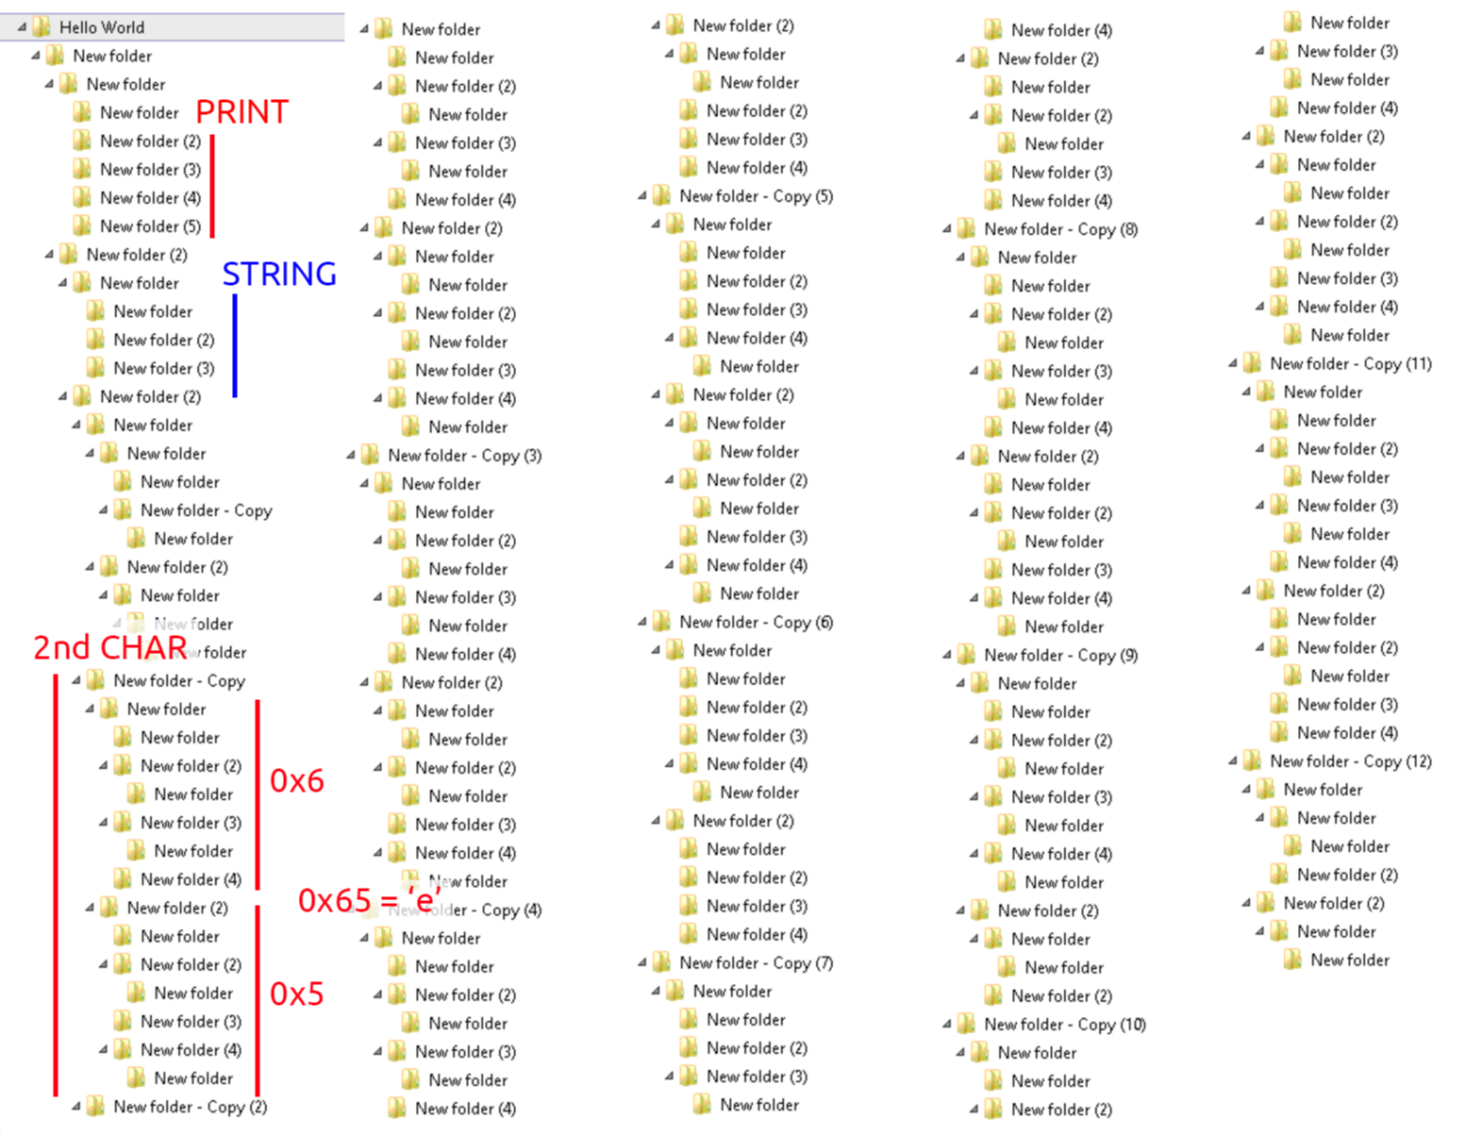
\includegraphics[width=\textwidth,height=\textheight,keepaspectratio]{PureFolders_HelloWorld_explained.png}
  \caption{Implementation of the traditional \lstinline{"Hello, world!"} program in the Folders programming language. \citep{temkin_daniel_2015}}
  \label{graphic:folders}
\end{figure}

Similar to architecture, software can hardly be separated from what it does, and yet fringe cases do exist in order to focus on under-examined aspects of how an artefact is traditionally thought. In architecture, particular structures do escape expected functional assessments in order to provide new understandings and new possibility, as in the construction of Renaissance follies (displaying symbolic value) or the modern pavillion (displaying technical prowess). Neither of these constructions abide by the traditional function of  architecture (sheltering, sustaining and sheltering life) but, precisely, these are exceptions confirming the rule, and these extreme examples also help to highlight the default standard, often taken for granted.

At the other end of the spectrum, we can consider code poems as the complementary opposite of such material investigations, arguing rather for the human expressiveness of programming languages. Here, the function is not effective—what actions does programming enable—but epistemological—what concepts does programming render.

The use of a language such as Perl in both hacky one-liners and full-fledged poems concludes our argumentation of how, along with technical environments, the social environment matters by providing a frame of understanding. We have shown both the variety and necessariness of functions in the aesthetic judgment of program texts, as they relate on such environments. Furthermore, we have shown that such function can be both material, in the sense of what technology can help us do, and epistemological, in the sense of what the technology can help us think about. We now conclude this chapter with an investigation into this latter part: the relational, cognitive function of aesthetics connecting aesthetics and ethics.

% FUNCTION IN AESTHETICS 8k
\subsection{Function in aesthetics}
\label{subsec:function-aesthetics}

% here, what i talk about is that, yes, aesthetics function as a cognitive device, both writer and reader.

% transition from east europe paper about ethics

Operating on the understandability of the ideas that are being presented through source code always implies a certain relation. This relation can be seen in the concept of \emph{niceness}, both from a human perspective and from a machine perspective. For instance, the Ruby community and their motto: "\emph{Matz is nice, and so we are nice}", sets up a particular context for a human-oriented appreciation of code, one whose syntactic properties is focused on human understanding rather than machine understanding and co-existence\footnote{We can also make a parallel with the \lstinline{nice} score of process on UNIX, further pushing this idea of cohabitation, this time from a machine perspective.}. The point here is that aesthetic programming, as a pleasing acitvity at the level of the sense and at the level of the intellect is as well a form of altruistic programming and ties back to a moral virtue mentioned in \ref{subsubsec:compression-habitability} \citep{fleetwood-boldt_matz_2020}. This moral dimension is introduced by the function that program texts have, since they have pratical implications and consequences, and are only autotelic at the edges (specifically, in hacking and poetry).

There is thus an effectiveness to source code aesthetics. A program text look nice because we know that its execution going to perform their function well, and that its arrangement will enable us to perform further functions—that is, its affordances signals that our needs are going to be met by its use. Similarly to the heuristic nature of aesthetics in mathematics \ref{subsubsec:beauty-mathematics}, aesthetics come into play both in the writing and reading of source code.

Writing is, in the moment of its doing, a broadly personal act. When a programmer writes some source code, they do so in a somewhat intimate manner: the only functional judges are onself and the machine, while the only aesthetic judge is oneself. Criteria for aesthetic judgment, at this point, include three axes: the accuracy of the action performed once the program is executed, the ability of the program text to express the concept that is being implemented, and the adequacy of this formal arrangement with the problem at hand—that is, the idiomaticity and elegance of the program text as a solution. Indeed, functional entities appear graceful when they are free of features that are extraneous, or irrelevant in relation to their function. This translation of function into appearance in turn depends on the complementary position: reading source code.

Once a program text is written—that is, once an idea has been given form—the process of reading introduces new constraints for an aesthetic judgment. Reading a program text involves a process of decrypting the realized adequacy between intent, form and function. This amounts to identifying the semantic affordances, under the form of structure, syntax and vocabulary used by the writer(s) to communicate the ideal action of the program. Considering aesthetics as the sensory manifestation of a desire of expression, we put here a particular emphasis on the relationality of such expression. The position of the reader always involves an otherness with respect to the position of the writer\footnote{Even if both those positions are shared by the same individual over a certain period of time.}. Providing an aesthetic judgment from a reader's perspective thus involves establishing the elegance, fitness, and interest of a certain piece of source code. Things are functionally beautiful where their perceptual appearances are altered by our knowledge of their function \citep{parsons_functional_2012}—that is, artefacts are functionally beautiful when we know where to look, and how to look, implying a certain epistemic movement in the reader.

These properties of elegance, fitness and interest of a program text are all related to its function, with such function being a balance between ideal function and implemented function, expectations and reality. In order to establish a connection between form and function, particularly from a reader's perspective, one must first establish what the program text is about, what it does, how it does, and whether these three dimensions are congruent. Therefore, the translation from form to function involves the acquisition and construction of knowledge. As we have seen throughout this thesis, such a knowledge construction takes place through the establishment of mental spaces. The accuracy and habitability of such spaces both elicit aesthetic pleasure and enable further action within the functional context established by the program text. In this configuration, we can see the importance of the role played by aesthetics as enabling the mental processes, and the construction of mental spaces, representing a clear, distinct and particular computational (that is, functional and operating) idea.

% then back to goodman for knowledge communication and ethics --- this is where i miss my notebook

Concluding in the \emph{Languages of Art}, Goodman develops on the relationship between art and understanding. Specifically, he compares an artistic attitude, involving an aesthetic experience, with a scientific one:

\begin{quote}
  The difference between art and science is is not that between feeling and fact, intuition and inference, delight and deliberation, synthesis and analysis, sensation and cerebration, concreteness and abstraction, passion and action, mediacy and immediacy, or truth and beauty, but rather a difference in domination of certain specific characteristics of symbols. \citep{goodman_languages_1976}.
\end{quote}

As a crafted technical artifact borrowing from the characteristics of natural language symbol system, and executed by the machine, source code as a medium occupies a hybrid place between art and science. With a genealogy rooted in hard sciences, and with an ontological nature of functionality, it always involves the concept of correctness, a correctness which is always verified through execution. On the other side, the complexity of the computational systems being described, and the uniqueness of the syntax and semantics offered by the medium of source code that is a programming language, require a certain amount of expressiveness found in the use of metaphors to represent concepts from both the problem domain, and from computation itself.

A final specificity of program texts is that there are very often collaborative and open-ended, as represented by the open-source movement, which tends to make all program texts writerly texts. This double movement of readers being potential writers and writers being potential readers complicates an already complex matter. Since the audience can become the creator of modified functional technical systems, expressive devices also act as communicative devices, and thus take on a relational dimension. In turn, this relational dimension within a technical environment involves notions of skill and knowledge whenever the understanding of a program text is at stake, notions of pre-existing skill and knowledge which, in turn, vary from one individual to the next. The program text therefore acts as a bridge between the intent of the ideal version of the software, and the mental spaces constructed by a reader.

All source code aesthetics relate to a certain conception of function: either technical function, or social function, and more or less essential to aesthetic judgment (with poetry and hacks standing at the edge of software and research engineering). While these two understanding of function further impact the manifestations of source code, these manifestations are not just expressive, but also communicative, aiming at transmitting concepts from one individual through the use of machine syntax. Indeed, code that is neither functioning for the machine, nor meaningul for a human holds the least possible value amongst different combinations presented above.A program is always a program \emph{about something}, and therefore holds some intentionality, an intentionality which can, in turn, be made pleasantly graspable by a writer to a reader.

In the majority of cases of program texts, the expectation is to understand. The recogntion of the existence of the other as a reader and co-author, both a generalized other in the sense that anyone can theoretically read and modified code, but also as a specificied other, in the sense that the other possesses a particular set of skills, knowledge, habits and practices stemming from the diversity of programming communities. This stance, between general and particular, is one that shows the ethical component of an aesthetic practice: recognizing both the similarity and the difference in the other, and communicating with a peer through specific symbol systems.

\spacer

In conclusion, this chapter has argued first that programming languages provide a socio-technical linguistic environment. Acting first as an interface to the computer, programming languages, without overly-determining the practice of programmers or the content of what is being programming, nonetheless influence how it can be said, through idiosyncracies and stylistic devices.

Starting from John Cayley's framework of levels of literary analysis, we then present a layer-based approach to the points in which aesthetic decisions can take place in source code—that is, across structure, syntax and vocabulary. Broadening this approach, we then showed how these different levels involve an engagement with \emph{semantic layers}: between the human reader, the machine reader and the problem domain. A source code with aesthetic value is one which balances syntactic techniques, structural organization and metaphorical choices in order to communicate a socio-technical intent of a functional artefact.

Analyzing this role of function in the aesthetic judgment of source code, we explicited the two main contexts in which source code is written, as a way to further define how that intent can be judged. These, in turn, determine what kind of aesthetic judgment can be bestowed upon a particular program text. As we related to previous debates of the role of function within aesthetic appreciation, we specified the idiosyncratic status of source code as a medium: between technical and social, expressive and communicative, individual and collaborative. If the aesthetics of source code are highly contextual, they are also social, and as such help us highlight the ethical dimension of aesthetics.
\chapter{Conclusion}
\label{chap:conclusion}

%
% BITCH BE HUMBLE
%
% this is supposed to specify what we have found, why it's valuable, how it can be applied, what is new and exciting
% his will show how it has made a valid, and useful, contribution to knowledge.

A piece of source code, as the lexical representation of computational processes, themselves representations of worldly matters, is an ambiguous object. Such an object exists at the overlap of both human and machine comprehension, and is often hidden away by the executed processes of which it is the source. And yet, source code practioners, those who write and read code, agree on the existence of a certain sense of \emph{beauty} in source code.

The research aims of this thesis were to highlight the origins and implications of the aesthetic properties exhibited by varieties of source code. That is, we intended to show how aesthetic properties relate to other aesthetic fields, and what role they played in the existence and purpose of source code—with a particular focus on its relationship to function. Our methodology started from an empirical approach of looking at specific instances of source code, and on analyzing of the discourses surrounding and commenting these instances. From this initial study, we identified several lexical fields that programmers refer to when they evoke the aesthetic properties of source code—literature, architecture, mathematics and craft.

Along with this first research axis, we also noted how the aesthetic judgement in source code is closely tied to its fuctionality. Indeed, any aesthetic value is dependent on the correct behaviour of the source code; ugly code is related to its apparent bugginess and difficulty in engaging with it, while beautiful code implies that the actions resulting from the source code are conform to what the programmer had intended, along with being presented in the best possible way\footnote{Such a definition of a \emph{best possible way} is dependent on the social, cultural and economic spheres within which the code is produced.}. The aesthetic properties of source code are therefore those of a semantic representation of computational space-time, whose purpose is the effortless communication of the operations of the computer, the intention of the programmer(s) and the representation of the world.

\section{Findings}
\label{sec:findings}

The rest of this conclusion will address each of our initial research questions' findings, followed by an examination of the limitations and contributions to existing research on source code.

\subsection{What does source code have to say about itself?}
\label{subsec:conclusion-rq-1}

One of the gaps we identified in source code-related literature is that there was a missing overlap between a broad empirical approach and a robust conceptual framework, expliciting the nature of source's code properties. for instance the works of \citep{paloque-berges_poetique_2009,cox_speaking_2013} establish an overview of source code with explicit aesthetic properties, but rely on a remediating approach to assess source code as a literary-semantic tool, or as a discursive-political object, respectively. We intended to complement this initial work to highlight source-code-specific aesthetics—that is, formal manifestations with a communicative purpose.

Starting from trade literature on the topic, and complementing it by cases of close-reading, we have highlighted both structural and contextual specificities to source code. Building on existing work, we have found several properties which seem to be unique to source code. Altogether, these properties support our theory of source code as a material used to construct dynamic semantic spaces.

Conceptual distance is key at a structural level: correlated expressions, statements or variables that affect or depend on the same concept (e.g. a file operation or a user account), should be located close to one another in the source code. This counterbalances the entropic tendency of source code to tangle itself, such that the reader has to follow the convoluted machine path of execution, rather than the human conceptual grouping of executable statements.

% \begin{listing}
%     insert example / comparison here
% \end{listing}

The conceptual coherence, and thus its ease of understandability, is also manifested in \emph{conceptual atomicity} and \emph{conceptual symmetry}, respectively meaning that a given explicit fragment of source code should do only one thing and do it well, and that fragments of source code that do similar things should look similar as well. Also previously identified as \emph{separation of concerns}, these two principles allow for the abstraction of a given syntactic unit by grouping all the statements into a single action or declaration.

At the lexical level, source code operates on a multi-dimensional level. On the one hand, it operates on an axis that goes from \emph{global} to \emph{local}, whereby global tokens that are used, and are visible, across the whole application code are very explicitly named, sometimes in all uppercase, while local tokens, whose lifetime does not exceed a few lines, tend to be composed of just a few letters. Here, variable length and cap size is closely related to the concept of \emph{scope}, yet in a slightly looser way than from a strict programming language perspective. On the other hand, lexical tokens can belong to three different lexical fields. These lexical fields are whether a given token refers to (1) an individual meaning, (2) a machine meaning, or (3) a domain meaning. For instance, the names \lstinline{start_time}, \lstinline{UTC_UNIX_STRING_NOW} and \lstinline{meeting_time} might all refer to the same moment in time, yet from different perspectives. The first naming, as an individual meaning, is significant in a narrow context, for a narrow set of individuals at the moment of writing or reading. The second naming is a machine meaning, which refers to how that moment is perceived by the computer. The third is the domain meaning, which is how users (and not writers or readers of source code) will refer to that particular moment.

For some, a piece of source code which can choose a token that will balance these three meanings in order to convey these three senses of the value at hand will be considered aesthetically pleasing. For others, writing tokens at the extreme of either of these three poles can be considered as a marker of aesthetic success and expertise. For instance, code poets would tend to focus on the domain meaning, in which tokens are only referring to non-computing terms, evoke poetic concepts insted. Conversely, hackers share a standard for brevity and directness—by making their tokens as short as possible, e.g. reducing them to bytecode, they strive towards existing as close as the hardware the code will run on, and therefore display unsual feats of performance.

This context-sensitiveness brings us to another aspect of source code—that it is eminently dependent on communities of practice to establish what is beautiful code. With a strong ethos of craft running as a thread throughout each of these identified communities\footnote{Software engineers, scientists, hackers and poets}, well-written code is \emph{idiomatic code}. This implies that the reader and the writer both possess some knowledge of the specificities of the language or hardware that the code is being written with and executed with. This approach to craft thus resonates with a concept of mastery and technical excellence, but also with that of \emph{style}. Style, in this case, highlights the acknowledgment of the social existence of code: by choosing style as a group marker rather than as an individual marker, a source code is judge positively based on its altruistic ethical nature—even if that style is enforced by software itself.

In this research, we have shown that code exhibits specific aesthetic properties, whether they are judged as being positive or negative. We have also shown that these positive or negative judgments are themselves the results of specific communities of practices—argumenting for a social conception of an aesthetic value judgment.

More fundamentally, the aesthetic properties of source code are derived from a conception of code as a semantic material which in terms is assembled, and apprehended, as a spatial construct, rather than a strictly literary, mathematical, or architectural material. Code \emph{navigation}, code \emph{structure} or \emph{code} compression, are terms which all belong to a lexical field of spatiality; the aesthetic properties of source code are tightly related to this apprehension of conceptual spaces constructed from machine-readable lexical tokens represeting problem domains—or, in other words, \emph{thought-stuff} \citep{brooks_mythical_1975}.

\subsection{How does source code relate to other aesthetic fields?}
\label{subsec:conclusion-rq-2}

These aesthetic properties were formalized through an empirical approach, whose first stage included the identification of the different lexical fields that programmers referred to in order to justify their aesthetic judgments of source code. Specifically, we have identified references to literature, architecture, mathematics and engineering. Each of these were used as a metaphorical device in order to better qualify source code (e.g. "source code is \emph{like} literature\dots").

To which aspect of source code did these references map to? Overall, we have identified two main aspects: semantic compression and spatial expression. Semantic expression concerns the ability of a notation to express complex concepts through quantitatively and qualitatively simple combination, while spatial expression concerns the ability of source code to be structured in such a way that is both evocative (the broad shape of things have a relative connotation to what things do) and sustainable (the structuring of a function ensures that a given action will not have unexpected side-effects).

All of these references point to the fact that structure and expressivity are closely tied when it comes to source code. Furthermore, rather than being opposites of one another, each reference contributes to the purpose of source code aesthetics by clarifying the structure of the code at multiple levels and dimensions.

Literary aesthetics facilitate the comprehension of the scope of variables and of the intent of the programmer in relation with the problem domain. They denote the purpose and intent of specific values, expressions, declarations and statements in a natural language, with a potential both for poetic evokation, cryptic obfuscation, or plain misinterpretation. Despite Yukihiro Matsumoto and Donald Knuth's statements that writing source code is a literary art, this turns out to only be partially true: the most literary parts of source code—comments—are also the parts that are the most decoupled from the actual source code, and are entirely invisible to the machine.

A strictly literary understanding of source sets aside the particularities of the reading process of source code and the temporal control of the writer. A traditional, natural language literary work will assume a linear, front-to-back readership, while source code is defined by its potential ability to jump from any part of the text to any other part of the text. Given this radical difference, references to architectural aesthetics help to establish structural patterns of familiarity and spatiality. Even though it does not operate on concrete, "natural" space, the quality of the disposition and combination of the application components on the source code page enable a better navigation of the source code's conceptual space.

This reduction of a vast conceptual space to natural language representations, and presented as clear, delimited set of interrelated components  reveals the tension in source code between form, function, and the fundamental concepts of the function. In this respect, mathematical aesthetics enable the condensation of knowledge and insight in the least amount of tokens, minimizing noise, and related to poetic condensation. Particularly, this ability of representing complex ideas into simple terms is a process of \emph{compression} shared across poetry and mathematics, and resulting in an elegant structure.

This concept of elegance is also found at an overlap of mathematics and architecture, in the form of engineering. Robust, sparse and straightforward engineering is considered a beautiful achievement, one in which function, structure and skill are intertwined to produce the most with the least. Here, this definition of "the most" is not one based on performance or CPU cycles\footnote{As mentioned previously, the most efficient code is machine generated and human-unreadable.}, but rather on its easing of the human's cognitive burden in understanding and engaging with the technical object that is source code.

Ultimately, all of these elements relate to communication and cognition, and to how the (invisible) purpose and intent of the code can be communicated in (visible) lines of a language straddling the line between machine and human comprehension. Literature, architecture, mathematics and engineering all rely on formal tokens to refer to \emph{something else}, and their efficiency at doing so can be assessed by the reader's correct or erroneous estimation of what are the fundamental concepts of what is being communicated to them. Keywords, tokens and beacons are all elements which have been found to structure the writing and reading of source code, allow the programmer to establish a cognitive map of the abstract structure of the program text.

\subsection{How do the aesthetics of source code relate to its functionality?}
\label{subsec:conclusion-rq-3}

This final correlation of aesthetics the communication of intent and purpose now leads us to address our third research question: the connections between form and function in source code. we have shown that, in the case of software engineers, aesthetics can be used to facilitate understanding in a functional context, or that, in the case of hackers, aesthetics can be a display of a deep understanding of the material at hand. As for scientists and poets, aesthetics perform a role of compression of complex concepts (be they scientific or poetic) into a concrete form.

However, the most crucial aspect of the aesthetics of source code is that they are rendered moot if the executed code does not perform as intended. In this case, there is a mismatch between what the original programmer(s) intended, and how the actual machine perfomance. This actuality can be referrenced in comments or documentations\footnote{Such as "TODOs" notes or open issues in tracking software.}, but lacks any guarantee of synchronization: the programmer might say something and the machine do something different, and it is not \emph{clear} what exactly is that difference. In this case, the program text, as the only component of software taken into account by the computer, is also the only canonical source of investigation into restoring the nature of the programmer—its function.

In this sense, the quality of an aesthetic property can be judged on whether it adequately represents a given concept, behaviour or intent\footnote{These are indeed three different things, but all involve some sort of some aspect of being remote for direct grasp.}. The unique aspect of this aesthetic judgment of source code is that there are indeed to judges: the human(s) and the machine, whereby the possibility for human assessment is dependent on the machine assessment. In all the different groups of writers identified, \emph{correctness} always conditions \emph{pleasantness}.

This is only verified to a certain extent for poets, who do not require a program text to be functional in the machinic sense in order to be given an aesthetic value. Still, in the case that the poet does write a syntactically correct text from a machine perspective, and a semantically evocative text from a human person, the artistic quality of the work created emanates from this technical feat. This dual display of skill relates to a conception of art as a connection between the technological and magical highlighted in subsection \ref{subsubsec:software-relational}. Displaying artistic creativity within source code can thus be seen as a way to enchant the technology of software, by representing it as a technically excellent crafted object.

This tight coupling of function and appearance, something already very present in modernist architecture and explored in section \ref{sec:arch-understanding}, echoes across theories of art as a language system used to express complex ideas, and practices of craft and toolmaking. Source code, while remaining subject to function, allows for a certain versatility in the expression of the concept (ranging from explicit to implicit) and, in turn, this expressivity depends on a given level of skill and practice in the idiosyncracies of the languages used. Related to our findings on the diversity of communities who read and write code, these communities are defined based on the purpose of the code they write, but there also exists a set of communities which are organized around the specific language that they use. The proficiency in a language involves a "right way to do things", and hints at the fact that there is a certain level of expertise is needed to assess the quality of the aesthetic properties of a source, and that the novice cannot be expected to provide an informed aesthetic value judgment.

\section{Contribution}
\label{sec:conclusion-contribution}

Overall, this thesis has aimed at showing that the formal properties of source code as a specific medium have a close relationship to \emph{episteme}, itself conjugated in various contexts.

Because software, underpinned by source code, belongs first and foremost to the technological realm, embodying a function and an intent of what should be achieved, aesthetics are inscribed within this technological essence by enabling the communication of the complex ideas which constitute the basis of software (its ideal version, as opposed to its implemented version, and its process of implementation, as opposed to its result).

While psychological studies and consolidated practical knowledge have shown that particular kinds of layout and presentation are beneficial to program understanding (see section \ref{subsec:psychology-programming}), this is only one aspect of the system of aesthetic properties. Aesthetic values in source code are also based on the \emph{context} in which said source code is written or read. These values, while varying, are nonetheless recurrently depending on the relation with the program, the machine, and the audience of the program, as well as the intent of the use.

In order to achieve this epistemic function, and due to software's ambiguous nature as an \emph{abstract artifact}, a variety of aesthetics domains are summoned by programmers in order to make sense of what they describe as occurences of software beauty. Looking specifically at the overlap of these domains, we have shown that each aim at facilitating a transition between the surface-level syntax immediately accessible to the reader to the deep-level semantics of the topic at hand. Respectively, literature aims at evoking themes and stories (section \ref{sec:aesthetic-literature}), architecture aims at evoking atmospheres and functions (section \ref{sec:arch-understanding}), while mathematics tries to communicate theorems (\ref{sec:aesthetic-mathematics}) and engineering focuses on structural integrity and efficiency (\ref{subsec:aesthetic-engineering}), with all domains above modulated by an approach to craft.

From the perspective of aesthetic theory, these findings also contribute to a conception of aesthetics as a communicative endeavour. Specifically, we have shown that the concept of aesthetics amongst programmers is not seen exclusively as an end to all things, but rather as a possible means to represent \emph{something} to \emph{someone}. As such, aesthetics acts as an expressive interface between a concept and two distinct individuals\footnote{The assumption specific to source code being that the same individual differs over time.}. Located within the particular techno-social environment of source code, this communicative role is also subject to relatively clear assessments of success or failure. A successful communication is a communication which is correctly interpreted, whereby the original ideas transmitted from the writer via the program text are found in an equivalent representation in the reader. Here, the interpretation is, at minima, what the program does, and what the program intents to do, things that might not always be aligned, resulting in the provision of agency in correctly predicting the implications of the program's operations and in the ability to correctly modify the program.

The contributions of this thesis have therefore been in the development of an aesthetic understanding of source code through an interdisciplinary analysis of a discourse analysis, drawing across media studies (from literature to software studies), science and technology studies and aesthetic philosophy. These discourses were composed of a corpus of both program-texts and commentaries and analyses by practicioners of those program texts—reading and analyzing  XXXX INSERT EXACT NUMBER XXXX selected source code snippets. In this sense, we have extended on the contributions of Paloque-Bergès and MacLean and Cox by applying on their concepts of \emph{double-meaning} and showing how this co-existence of computer meaning and human meaning extends beyong the more creative writings of source code, and across communities of source code writers.

In doing so, we have also confirmed and extended Piñeiros' work on describing code aesthetics as instrumental action, bridging his field of research of software developers with other kinds of source code, and confronting it with specific example. While Piñeiro's work thoroughly explores programmers' perspectives, it does not extend its findings to other aesthetic practices mentioned by programmers—by connecting it to literature, architecture, mathematics and engineering, we inscribe the practice of programming within a wider array of creative practices.

I proposed a conceptualize of code as semantic matter, from which executable structures are built. This approach builds on Katherine Hayles' distinction between the media properties of print and code—the former being flat, the latter being deep. The contribution was to enrich our understanding of what code depth is made of, and how syntactical tokens create conceptual structures.

I offered a typology of how to exert aesthetic properties in code, based on the purpose of aesthetics as a communicative endeavour with specific outcomes. This complements the perspectives provided in the Oram and Wilson's edited volume \citep{oram_beautiful_2007}. Instances of beautiful code have been given a theoretical framework as a criterai for belonging to the category of exhibiting positive aesthetic properties, beyond their praise by highly-skilled practitioners.

Through an empirical take, we have also qualified how Florian Cramer and his approach to source code as a form of magic relies on very concrete technical processes and habits across practices of source code writing. Building on the conception of Alfred Gell of art as the enchantment of technology, we have explicited what exactly are the complex technical hurdles and associated skills required to understand software (section \ref{subsec:software-complexity}). If there is magic in software, it is also manifested through the aesthetic appreciation of source code, particularly through hacking (section \ref{subsec:hackers}) and code poetry (section \ref{subsec:poets}), and examplified in works like \lstinline{forkbomb.pl} (see listing \ref{code:forkbomb}).

\begin{listing}
    \inputminted{perl}{./corpus/forkbomb.pl}
    \caption{forkbomb.pl is an artwork in the exhibited sense of the term, displaying conciseness along with expressive power through its technical expansion}
    \label{code:forkbomb}
\end{listing}

Finally, this thesis has contributed to a text-based approach to software aesthetics, as compared to execution-based approaches, in which source code syntax and semantic tend to be set aside. Within those studies of code-dependent aesthetics, such as interface design \citep{fishwick_aesthetic_2000} or creative coding \citep{cox_aesthetic_2020}, the aim was to provide an account of how code, the material itself, offers in terms of representational specificities to enrich those studies.

Without directly contradicting any of the work mentioned in our literature review (see \ref{subsec:literature-review}), our conclusions offer a detailed account of the material origins upon which subsequent interpretations of code are based.

\subsection{Limitations}
\label{subsec:conclusion-limitations}

The first and most obvous of this limitation is that a lot of source code is not accessible. While originally a freely-circulating commodity, the emergence of proprietary software at the dawn of the 1980s \citep{hassett_impact_2012} has drastically limited free and open access to source code. As such, most of the source code written by software engineers in a commercial context remains confidential. For hackers, due to the nature of the work as an \emph{ad hoc} and localized practice, few examples are made publicly available, as they are often enmeshed in more commercial projects, themselves subject to property restrictions.


A second limitation is the expertise level required not just in programming, but in idiomaticity—that is, in knowing how to best phrase an action in a specific languages, as addressed in subsection \ref{subsec:idiomaticity}—and, to a lesser extent, in the relevant problem domains. This implication of having already a solid grasp on the technical and problem context can have affected the expositions of aesthetic judgments that I have given in this thesis. Consequently, it is inevitable that other experts programmers might have different opinions given their personal styles and backgrounds.

Finally, our focus on the knowledge-component of both aesthetics and source code has led us to venture into the application of cognitive sciences through empirical studies to fields such as programming, literature or architecture. Since this is still a burgeoning endeavour, in active research,  some of the connections evoked by the current literature between code and cognition, or beauty and cognition are still bound to evolve.

\section{Opening}
\label{sec:opening}

Firmly grounded into aesthetic philosophy, this thesis has nonetheless aimed at expanding the domain of what is traditionally considered beautiful, and how it is considered so, by examining its relations with function and knowledge. Resulting from an interdisciplinary approach, the outcomes of this research therefore have some impact  on both the arts and sciences in general, and programming in particular.

Deliberately eschewing notions of the artistic in favor of the beautiful, the definition work at the beginning of this thesis implied that studies of beauty decoupled from art can be rich and fruitful, revealing a plethora of practices focusing on making something nice, rather than, e.g., gorgeous. This thesis is therefore inscribed in aesthetics of the everyday, and can suggest ways to apply aesthetic judgments to objects of study usually excluded from such. Additionally, we have shown how such objects—source code—possess mechanics of meaning-making of their own, enabling unique semantic structures.

Conversely, we also consider implications for programmers and craftspeople. Not that they need this work to realize that aesthetics and functionality are deeply intertwined, but rather as an explicit account of the ways in which this entanglement happens. For programmers, keeping in mind notions of scale, distance and metaphor within a particular source code would support better work. For other creators, we hope this would encourage them to investigate what is it that makes their material unique, and how it relates to other disciplines.

Ultimately, this work also has ethical implication. Knowledge, by enabling one's agency, supports and encourages good work, as opposed to meaningless labour. By organizing program texts in such a way that the next individual can discover and understand underlying concepts transmitted through the medium of source code, one engages in an ethically altruistic behaviour, as opposed to self-reflexive references.

\spacer

In closing, we see two main directions which can unfold form this thesis, either exploring the poetics of code, or the intricacies of cimputer-readable knowledge management.

The unfolding of digital media in the second half of the twentieth century has been seen as an epochal shift, along with other technologies of information reproduction and diffusion. However, computational media is specifici insofar as it can be compressed and unfolded under various forms (from electricity to three-dimensional graphical environments and highly-dimensional vector spaces in recent machine learning approaches). How does the shape of software impact knowledge management and transmission, not just for programmers, but for end users as well, starting from those in the information sciences such as librarians, educators, journalists, researchers, and expanding to anyone engaging in a meaning-making work within a computer environment. While aesthetics can help to signify complex concepts within source code, do those concepts translate at other interface levels, or do these subsequent levels hold aesthetics principles of their own?

In terms of poetics, or how the particular structure of a text has a particular effect on an audience, the question would be to which extent does source code structure model and affect the "real world"\footnote{Throughout this work, we have been referring to the "real world" as the problem domain.}. Particularly in terms of  time and space, as we have seen how the execution of source code enegage in a deeply different scale of both components of our experience of reality. In terms of moddelling, we could ask does a particular data structure, in how it is written, reveal social, political and economical agency? To what extent do languages such as Rust, Java or JavaScript influence the programmer's perception of the world? Could that effective impact be observed in an empirical manner? This move from form to consequence would look at an impact beyond programmers and at a broader audience. This relationship between form-giving and meaning-making in digital environments might start with those who write source code and compose electrical circuits, but affect all who engage with computers.


\bibliographystyle{./apa-good.bst}
\bibliography{thesis.bib}

\listoflistings

\end{document}
